% This variant is used for web PDF version of the book.
% Can be compied with XelaTeX:
% * TL 2013 or later

% TODO export all Tikz pictures to separate standalone TeX files for HTML build
% TODO apply letterspacing for titles: \\addfontfeature\{Style=TitlingCaps\} or \\addfontfeature\{ WordSpace = 1.1 \} or \\addfontfeature\{LetterSpace=2.0\}
% TODO add small caps
% TODO check italic and bold usage
% TODO redraw data-locality picture

\documentclass[a5paper,11pt,twoside,titlepage, numbers=endperiod]{scrbook}

\typeout{Copyright 2014 Grigory Rechistov and the contributors.}
\def \documentversion {2.11$\beta$} % increment and don't forget to update history.tex



% A switch to change between document rendering options
\usepackage{etoolbox}

\newtoggle{webpaper}
\toggletrue{webpaper} % Must be true for Web-PDF

\newtoggle{htmlpaper} 
\togglefalse{htmlpaper} % Must be false for non-HTML builds

\newtoggle{showanswers} % An option to show answers in quizes.
\togglefalse{showanswers}

\newtoggle{inappendix} % we are now in appendix
\togglefalse{inappendix} % ... but not yet

% Create vector pictures from TikZ environments
\newcommand{\inputpicture}[1]{\input{#1}}

\usepackage[top=2.0cm, bottom=2.0cm, left=1.84cm, right=1.5cm, footskip=1cm]{geometry}
\pagestyle{plain} % no headers, page numbers in footers

% Copyright (c) 2016 Grigory Rechistov <grigory.rechistov@phystech.edu>
% This work is licensed under the Creative Commons Attribution-NonCommercial-ShareAlike 4.0 Worldwide.
% To view a copy of this license, visit http://creativecommons.org/licenses/by-nc-sa/4.0/.

\usepackage{fontspec}
\usepackage{xunicode} % some extra unicode support
\usepackage{xltxtra}

\usepackage{amsfonts}
\usepackage{amsmath}
\usepackage{longtable}
\usepackage{csquotes}

\usepackage{polyglossia}
\setdefaultlanguage[spelling=modern]{russian} % for polyglossia
\setotherlanguage{english} % for polyglossia

% Common settings for all fonts
% 1. Attempt to make fonts be of the same size
% 2. Support TeX ligatures like — = emdash, << >> = guillemets
\defaultfontfeatures{Scale=MatchLowercase, Mapping=tex-text}

% Use Computer Modern Unicode
\newfontfamily\russianfont{CMU Serif}
\setromanfont{CMU Serif}
\setsansfont{CMU Sans Serif}
\setmonofont{CMU Typewriter Text}

% Common packages, commands and their configuration

\newcommand{\abbr}{\textit{англ.}\ }
\newcommand{\todo}[1][]{\textcolor{red}{TODO #1}}


\usepackage{graphicx}
\graphicspath{{pictures/}} % path to pictures, trailing slash is mandatory.

\usepackage{hyperref}
\hypersetup{colorlinks=true, linkcolor=black, filecolor=black, citecolor=black, urlcolor=black , pdfauthor=Grigory Rechistov <grigory.rechistov@phystech.edu>, pdftitle=Программное моделирование вычислительных систем}

\usepackage{footnpag}
\usepackage{indentfirst}
\usepackage{underscore}
\usepackage{url}

\usepackage{listings}
\lstset{basicstyle=\footnotesize\ttfamily, breaklines=true, keepspaces=true }

\usepackage{listings}
\lstset{basicstyle=\footnotesize\ttfamily, breaklines=true, keepspaces=true}

\usepackage{tikz}
\usetikzlibrary{shapes, calc, arrows, fit, positioning, decorations, patterns, decorations.pathreplacing, chains, snakes}
\usepackage{bytefield}

% Load package and tune params

\usepackage{appendix}
\renewcommand{\appendixname}{Приложения}
\renewcommand{\appendixtocname}{Приложения}
\renewcommand{\appendixpagename}{Приложения}
\let\plainappendixpage\appendixpage
\makeatletter
\renewcommand{\appendixpage}{% Delete page number in appendixpage
  \begingroup
  \let\ps@plain\ps@empty
  \plainappendixpage
  \endgroup}
\makeatother

\iftoggle{webpaper}{
    % \usepackage[duplicate]{chapterbib}
    % A hack to mimic biblatex macro for bibtex
    % \newcommand{\printbibliography}[1][none]{\bibliographystyle{ugost2008s}{}\bibliography{./../phd,./../mine,../collection}}

    \usepackage[language=auto, bibencoding=inputenc, style=gost-numeric, backend=biber, maxnames=4, refsection=chapter, isbn=true, ]{biblatex}
    \addbibresource{./../phd.bib}
    \addbibresource{./../mine.bib}
    \addbibresource{./../collection.bib}
    \renewcommand*{\multicitedelim}{\addcomma\space} % grouped cites separated by commas not semicolons
} {}    % Bibliography to be added at the end, not per chapter


% Copyright (c) 2016 Grigory Rechistov <grigory.rechistov@phystech.edu>
% This work is licensed under the Creative Commons Attribution-NonCommercial-ShareAlike 4.0 Worldwide.
% To view a copy of this license, visit http://creativecommons.org/licenses/by-nc-sa/4.0/.

% Custom stylistic adjustments for KOMAscript and fixes for
% certain problems discovered over time.
% Most were found on Internet.
% Some may be obscure.

\tolerance=9999 % let the text underfull be ugly as hell, nobody cares.
\widowpenalty=9998 % try to avoid widow lines
\clubpenalty=9998 % try to avoid orphan lines
\emergencystretch=3cm

\usepackage{nameref}
\usepackage{enumitem} % continue enumeration 
\usepackage{subfigure}
\renewcommand*{\thesubfigure}{\alph{subfigure})} % only one bracket in subfigures
\usepackage{mdwlist} % compact itemize lists environment
\renewcommand{\labelitemi}{--}  % Use endash for itemized lists
\renewcommand{\dictumwidth}{0.5\textwidth}
\newcommand{\dictumtext}{\normalfont\normalcolor\sffamily\tiny}
\renewcommand{\dictumauthorformat}[1]{#1}
\setcounter{tocdepth}{2}

\usepackage[hang,flushmargin]{footmisc} % correct indent for footnotes
\usepackage{verbatim}

\usepackage{amsthm}
\newtheorem*{digression}{Замечание}

\renewcommand{\chapterheadstartvskip}{\vspace *{-\baselineskip }} % Move chapter titles higher
\setcapindent{0pt} % make multi-line captions to be not indented, save some space with this
\renewcommand{\captionformat}{~} % do not put colon after figures numbers
\usepackage[subfigure, titles]{tocloft}
\renewcommand{\cftchapleader}{\cftdotfill{\cftdotsep}} % Dots to TOC chapter titles
%\setlength{\cftaftertoctitleskip}{20pt}

\let\cleardoublepage\clearpage % do not start from even page
\setkomafont{pageheadfoot}{% Enforce header and footer to be correct.
    \normalfont\normalcolor\itshape\small\rmfamily
}
\setkomafont{pagenumber}{\normalfont\rmfamily} % fix KOMA bug when footer/header inherits font settings from main text.

\addtokomafont{caption}{\small}



% This file defines several commands originally present in 'exam' class.
% The definitions are quite dumb but are enough to make it possible to copy-paste between 
% a quiz document and this book.
% Generally it just maps stuff to enumerated lists.

% For appendix, we renew commands to show answers unconditionally. This all is done in a lame way.

\iftoggle{inappendix}{
    \renewenvironment{solution}[1][0]{\textbf{Решение.}\ }{}
    \renewcommand{\correctchoice}{\item \textbf{Решение.}\ }
    \renewcommand{\Questions}{Ответы\ }
}{
    \newcommand{\question}[1][0]{\item}
    \newenvironment{questions}{\begin{enumerate*}}{\end{enumerate*}}
    \newenvironment{choices}{\begin{enumerate*}}{\end{enumerate*}}
    \newcommand{\choice}{\item}

    \iftoggle{showanswers}{ % show answers
        \newenvironment{solution}[1][0]{\textbf{Решение.}\ }{}
        \newcommand{\correctchoice}{\item  \textbf{Решение.}\ }
    }{% do not show answers
        \let\solution=\comment
        \let\endsolution=\endcomment
        \newcommand{\correctchoice}{\item }
        \newcommand{\Questions}{Вопросы\ }
    }
}


\begin{document}

\makeatletter\renewcommand\@biblabel[1]{#1.}\makeatother

\pdfbookmark{Титульный лист}{title}

\newlength{\centeroffset}
\setlength{\centeroffset}{-0.5\oddsidemargin}
\addtolength{\centeroffset}{0.5\evensidemargin}

\thispagestyle{empty}
\vspace*{\stretch{1}}

\begin{center}
	{\Huge\textsc{Программное \\ моделирование \\ \vspace{3pt} вычислительных систем}}
	\vspace{1cm}\\
	{\Large\textsc{Учебное пособие}}
\end{center}

% insert version number
\vspace{\stretch{1}}
\noindent\hspace*{\centeroffset}\makebox[0pt][l]{
	\begin{minipage}{\textwidth}
		\flushright
		Версия~\documentversion \\
		\today\\[3cm]
%		\iftoggle{hasquiz}{Вариант с контрольными вопросами}{}
	\end{minipage}
}
\pagebreak

% Insert CC BY NC SA notice for the web version
\thispagestyle{empty}
\begin{small} 
Copyright \copyright~~2011, 2012, 2013 Grigory Rechistov and the contributors.  All rights reserved.
\begin{center}
	
\includegraphics[width=0.2\textwidth]{../cc-by-nc-sa.png}
\end{center}

Данный вариант произведения распространяется по лицензии Creative Commons At\-tri\-bu\-tion-Non\-Com\-mer\-cial-Share\-Alike (Атрибуция — Некоммерческое использование — С сохранением условий) 3.0 Непортированная. Чтобы ознакомиться с экземпляром этой лицензии, посетите \url{http://creativecommons.org/licenses/by-nc-sa/3.0/} или отправьте письмо на адрес Creative Commons: 171 Second Street, Suite 300, San Francisco, California, 94105, USA. 
Полный список авторов и благодарностей см. в секции~<<\nameref{chap:contrib}>>.

Все зарегистрированные торговые марки, названия и логотипы, использованные в данных материалах, являются собственностью их владельцев. Представленная точка зрения отражает личное мнение авторов, не выступающих от лица какой-либо организации.
\end{small}


\tableofcontents

\chapter*{Об этой книге}\label{chap:contrib}

Главы данной книги соответствуют лекциям курса <<Основы программного моделирования ЭВМ>>, читаемого в Московском физико-техническом институте.

Нам очень важно мнение читателя. Если вы обнаружили опечатку, стилистическую, фактическую ошибку, которые c большой вероятностью встречаются в тексте, или имеете замечания по содержанию и предложения по тому, как можно улучшить данные материалы, то просим сообщить об этом по e-mail 

\begin{center}
\href{mailto:grigory.rechistov@phystech.edu}{\texttt{grigory.rechistov@phystech.edu}}
\end{center}


\section*{Предыдущие издания книги}

Над первыми двумя изданиями книги работал следующий коллектив авторов: Г.~С.~Речистов, Е.~А.~Юлюгин, А.~А.~Иванов, П.~Л.~Шишпор, Н.~Н.~Щелкунов, Д.~А.~Гаврилов.

Актуальная версия текста данной книги доступна в Интернет по адресу:

% \url{http://iscalare.mipt.ru/materials/course_materials/}.
{\scriptsize\url{http://atakua.doesntexist.org/wordpress/simulation-course-russian/}}

\section*{Благодарности}

%\dictum{}

Авторы выражают благодарность всем студентам-слушателям курса. Следующие люди сообщали свои замечания и предлагали исправления к тексту книги: Илья Куприк, Денис Шиляев, Денис Лытов, Анатолий Костин, Виталий Антонов, Даниил Альфонсо, Дмитрий Бородий, Иван Андреев, Наталья Иванчикова, Марина Шимченко, Максим Кузнецов, Святослав Кузьмич, Егор Кривов, Кирилл Ашейчик, Амир Аюпов, Даниил Саргин, Леонид Снегирёв, Александр Кравцов, Валерий Конычев, Всеволод Ливинский, Александра Цветкова.

Некоторые секции книги были первоначально опубликованы как посты на сайте Хабрахабр: \url{http://habrahabr.ru/company/intel/blog/}. Здесь они включены в адаптированном варианте.




\chapter*{Предисловие}\label{overview}
\addcontentsline{toc}{chapter}{Предисловие}

\dictum[Хорхе Луис Борхес]{Мы легко принимаем действительность, может быть, потому, что интуитивно чувствуем: ничто реально не существует.}


Симулятор, эмулятор, модель ЭВМ --- под этими понятиями подразумевается компьютерная программа, способная имитировать работу некоторой реальной вычислительной системы (рис.~\ref{fig:idea}). Процесс работы такой программы именуется \textit{симуляцией}, и подразумевает изучение эволюции состояния модели во времени, отражающей изменения в поведении и состоянии изучаемого аппаратно-программного комплекса.

\setcounter{chapter}{1} % a hack for not to have zero numbered figure
\setcounter{figure}{-1}
\begin{figure}[tp]
    \centering
    % \includegraphics[width=\textwidth]{./idea-crop.pdf}
    \begin{tikzpicture}
      
        \node[inner sep=0pt] (rack-system) {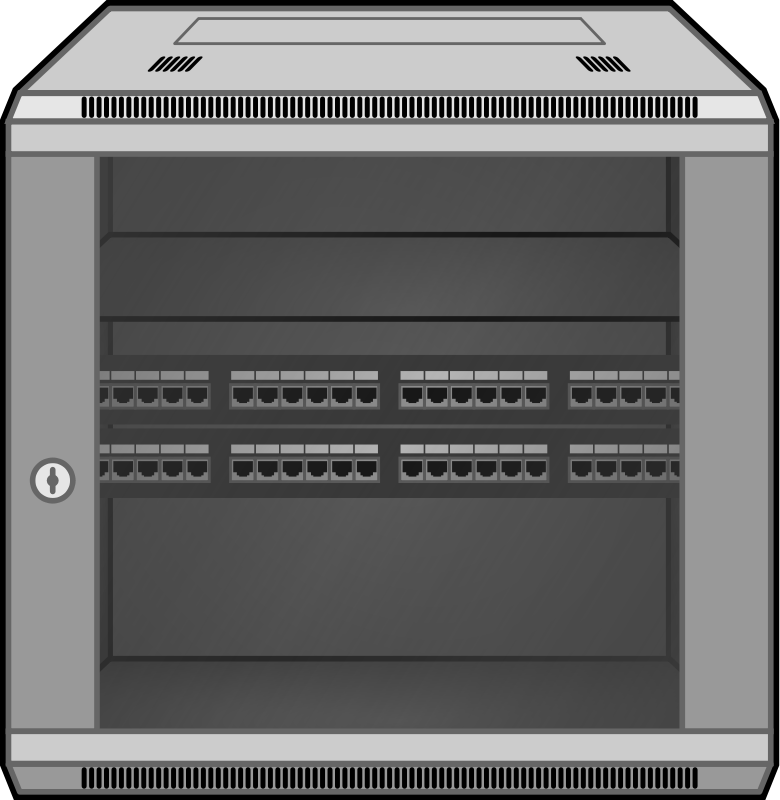
\includegraphics[width=2.5cm]{rack-system.png}};
        \node[above=0cm of rack-system, font=\footnotesize] {Модель};
        \node[cloud, draw, aspect=1.5, text width=3.2cm] at (rack-system) (cloud) {};
        
        \node[right=2cm of rack-system, yshift=-1cm] (laptop) {
\includegraphics[width=2.2cm]{laptop.png}};
        \node[color=white, anchor=base, font=\footnotesize, yshift=0.2cm] at (laptop) {\textbf{Симулятор}};
        
        \path[] (cloud) -- (laptop) node[draw, pos=0.6, sloped, single arrow, text width=0.4cm] {};
    \end{tikzpicture}
    \caption[Основная идея симуляции]{Основная идея симуляции. Модель некоторой вычислительной системы в виде программы исполняется на компьютере другой конфигурации и/или архитектуры}
    \label{fig:idea}
\end{figure}
\setcounter{chapter}{0} % restore the chapter counters
\setcounter{figure}{0}

Существует несколько различных трактовок терминов \textit{симуляция} и \textit{эмуляция}. Наиболее общеупотребительное понимание различия между ними таково: симуляция --- некий процесс, имитирующий внешние проявления системы, внутреннее его устройство при этом не повторяет детально оригинал; эмуляция же, кроме внешних эффектов, представляет внутреннюю структуру, максимально приближенную к оригинальной системе. Размышляя над этими определениями, можно заметить, что смысловая грань между ними очень тонка и в основном зависит от того, насколько глубоко мы готовы <<заглянуть>> в модель и в объект моделирования при исследовании; при этом эмуляция может легко оказаться симуляцией. По этой причине далее всюду в тексте понятия \textit{симулятор}, \textit{эмулятор}, \textit{модель} будут использоваться взаимозаменяемо, и их значение будет больше зависеть от контекста обсуждения, чем от строгих определений.

Существующие модели компьютеров различаются множеством параметров, таких как фокусировка на различных аспектах работы изучаемой системы, точность соответствия поведения реальной и моделируемой системы, скорость работы, внутренний дизайн и внешние интерфейсы к нему, задействование различных оптимизационных техник, эвристики, заложенные в процесс симуляции.

Для максимально эффективного усвоения материала книги читателю рекомендуется иметь начальные знания по архитектуре ЭВМ; рекомендуется обратиться к великолепной книге~\cite{patterson2012rus}. Желательно понимание читателем общих принципов работы операционных систем, а также знакомство как  минимум с одним языком программирования.

Нельзя не упомянуть книгу о виртуальных машинах, которая вдохновила авторов на написание этой работы~\cite{DBLP:books/daglib/0013597}. Знакомство с ней также настоятельно рекомендуется всем читателям, желающим глубже разобраться в вопросе виртуализации.

Необходимо понимать, что методика моделирования применима не только к изучению вычислительных или цифровых, но и практически к любых технических, социальных или каких-либо иных систем. Читателю, желающему расширить своё понимание метода, рекомендуется книга~\cite{system-modeling}.

В главе~\ref{chapter01} дано описание областей применения симуляторов, введены ключевые понятия и приведены примеры использования технологии симуляции в прошлом и в настоящее время.

%В главе~\ref{chapter02} описаны существующие в настоящее время программные решения, используемые в исследованиях, разработке и коммерческой эксплуатации.

В главе~\ref{chapter03} приводится пример построения простого симулятора процессора, основанного на интерпретации инструкций.

В главе~\ref{chapter04} представлены дальнейшие пути увеличения скорости моделей процессоров, такие как двоичная трансляция и аппаратная виртуализация.

В главе~\ref{chapter05} рассматривается исследование вычислительных систем с помощью трасс исполнения --- записи истории внешних событий.

%Глава~\ref{chapter06} знакомит с альтернативными подходами изучения ЭВМ с помощью различных методик: теории сетей центров обслуживания; сбора и проигрывания трасс событий; вероятностного моделирования.

Глава~\ref{chapter07} описывает подходы к симуляции системы с множеством устройств, включая многопроцессорные системы.

В главе~\ref{chapter08} рассматриваются подходы к параллельной симуляции; показывается, что эффективная и корректная реализация таких систем возможна, но в общем случае довольно сложна.

В главе~\ref{chapter09} описан подход к потактовой симуляции, обусловленный иным характером обработки событий в системе и потому отличный от ранее рассмотренных.

В главе~\ref{chapter10} показываются примеры организации хранилищ внутреннего состояния устройств, а также возможные для них оптимизации.

В главе~\ref{chapter11} кратко рассматриваются назначение и устройство сверхоперативной памяти (кэш-память), а также подходы к её моделированию.

В главе~\ref{chapter12} определяются существующие языки, используемые для написания моделей устройств, а также показывается их связь с языками, задействованными на поздних фазах, при проектировании устройств.

Глава~\ref{chapter13} знакомит с особенностями обеспечения взаимодействия симуляции с внешним физическим миром.

В главе~\ref{chapter14} даётся теоретический критерий возможности эффективной виртуализации вычислительных систем; затем проверяется соответствие ряда современных архитектур процессоров этому условию.


\newpage

\section*{Обозначения}

Всюду в тексте данной книги применяются следующие шрифтовые выделения и обозначения.

\begin{itemize*}
    \item Обычный текст используется для основного материала.
    \item \texttt{Моноширинный текст} вводится для исходных текстов программ на различных (псевдо)языках программирования, выделения ключевых слов, имён регистров устройств, листингов машинного кода.
    \item \textit{Наклонный текст} служит для выделения новых понятий.
    \item Числа в шестнадцатеричной системе счисления имеют префикс \textbf{0x} (например, 0x12345abcd), в двоичной системе счисления --- суффикс \textbf{b} (например, 10010011b).
\end{itemize*}

При введении терминов, заимствованных из английского языка и не имеющих известных авторам общепринятых переводов на русский, в скобках после них будут указываться оригинальные иностранные выражения.

\begin{digression}
    Параграфы, оформленные таким образом, являются необязательными для понимания курса и введены для того, чтобы показать порой неочевидные связи между приёмами моделирования и различными научными идеями и теориями.
\end{digression}

\iftoggle{webpaper}{
    \printbibliography[title={Литература}]
}{}



\chapter{Применение программных моделей}\label{applications}

\dictum[Станислав Лем. Кибериада. Сказки роботов]{\dots цифровая машина, получившая непосильное для неё задание, вместо того, чтобы заниматься решением проблемы самой, строит, если перейдён определённый порог, называемый барьером мудрости, следующую машину\dots }

\section{Введение}

Разработка новых узлов вычислительных систем, таких как центральные процессоры, графические карты и сопроцессоры, наборы системной логики, сетевые карты, а также проектирование вычислительных комплексов и средств их взаимодействия, являются сложными и длительными процессами. Сложность эта обусловлена многими факторами, среди которых можно выделить следующие.

\begin{itemize*}
\item Большое число составляющих систему устройств со сложными взаимосвязями, как явными, так и неявными, скрытыми или даже паразитными.   

\item Необходимость сохранения обратной совместимости с уже существующим оборудованием, дополнительно усложняющая дизайн.

\item Необходимость обеспечения поддержки аппаратуры программными продуктами, помогающими раскрыть их полный потенциал: драйверами для операционных систем, компиляторами, профилировщиками и др. средствами разработки.

\item Необходимость знать характеристики новой технологии (например, производительность, мощность энерговыделения, размеры) как можно раньше, чтобы принимать обоснованные в рамках рыночной конкуренции решения о целесообразноcти создания продуктов на её основе.

\item Важность выявления ошибок проектирования на ранних стадиях. Стоимость исправления недостатков резко возрастает вместе с этапом проектирования, на котором они были обнаружены. Исправить ошибку в описании на бумаге в начале проекта несоизмеримо дешевле, чем отзывать партии бракованных изделий, уже изготовленных по спецификациям, содержащим изъяны (рис.~\ref{fig:error-cost}).

\end{itemize*}

\begin{figure}[htb]
    \centering
	\inputpicture{drawings/error-cost}
    \caption[Рост стоимости исправления ошибки с фазой проектирования устройства]{Рост стоимости исправления ошибки с фазой проектирования устройства. Различные этапы проектирования могут перекрываться во времени, однако каждый из них подразумевает всё большие вложения ресурсов. Ошибки в уже выпущенном продукте могут повлечь за собой существенные финансовые и имиджевые потери для допустившей их компании}
    \label{fig:error-cost}
\end{figure}

По этим причинам широко используется подход, когда разработка нового устройства предваряется созданием и сопровождается использованием его компьютерных моделей, способных с различной точностью проявлять себя так, как работает реальное устройство. Построенные согласно этим принципам инструменты различаются назначением, точностью соответствия реальной аппаратуре, количеством моделируемых и конфигурируемых параметров, скоростью выполнения, внутренней организацией и принципами работы. Даже не полностью соответствующая реальности модель может быть практически полезной.

\begin{digression}
Моделирование возможно благодаря применению общесистемной методики борьбы со сложностью --- модульностью подсистем и абстракцией их функций. Устройства, входящие в состав компьютера, соединяются между собой через строго определённые интерфейсы, диктующие лишь то, что будет передаваться через них и какой тип результата будет возвращён, но не определяющие, что будет располагаться на другом конце. Это позволяет оборудованию различных производителей быть совместимым друг с другом без необходимости раскрытия внутренней документации конкурентам. Также это позволяет подставлять вместо реальных устройств их модели. Более того, по разные стороны интерфейсов мы можем размещать модели различных подсистем, таким образом создавать полную модель всего компьютера, компоненты которой <<не знают>>, что за интерфейсом скрывается не реальное устройство, а его модель~(рис.~\ref{fig:interface}).

\end{digression}

\begin{figure}[htp]
\centering
\inputpicture{drawings/interface}
\caption[Соединение компонент сложной системы через интерфейсы]{Соединение компонент сложной системы через интерфейсы, определяющие форматы запроса и отклика, но не специфицирующие детали реализации необходимой функциональности. Это позволяет заменять некоторые или даже все части такой системы на программные модели}\label{fig:interface}
\end{figure}

\section{Применения моделей компьютеров}

Перечислим некоторые способы практического применения программных моделей.

\begin{description*}
    
\item[Раннее обнаружение ошибок проектирования.] Программирование --- процесс значительно менее затратный, чем испытания реального железа, и что куда важнее, исправление ошибки в программе занимает минуты, тогда как повторный выпуск опытного образца аппаратуры может занять месяцы. 

\item[Написание сопутствующего аппаратуре ПО.] Ранняя доступность модели устройства позволяет использовать её для разработки драйверов, прошивок (таких как BIOS и UEFI~\cite{uefi-itj}) и даже операционных систем и компиляторов параллельно с разработкой самого устройства. В наше время нередка ситуация, что драйвера для нового оборудования готовы и отлажены ещё до официальной доступности предназначенного для них оборудования.

\item[Построение и исследование экспериментальных решений.] Моделирование позволяет быстрее и дешевле  изучать пространство проектирования (\abbr design space) для определения параметров, при которых устройство или система будет иметь наилучшие характеристики. Для исследователей интерес часто представляют количественные характеристики новых систем, такие как скорость работы, степень загруженности подсистем, потребление энергии и т.п. Иногда подобный анализ можно провести и без симуляции, используя аналитические методики, теорию массового обслуживания, экстраполяцию измерений на существующей аппаратуре и т.д. Однако моделирование даёт наибольшую гибкость.

\item[Качественно-функциональные свойства.] Под этим тер\-ми\-ном понимается изучение, работает или нет новая технология в принципе, безотносительно её скоростных характеристик. В этом случае альтернатив симуляции практически не остаётся, поскольку необходимо изучить функционирование системы.

\item[Выполнение программ на <<неродной>> архитектуре.] В этом случае модель обеспечивает прослойку, позволяющую выполнять приложения без перекомпиляции на машинах, изначально не предназначенных для исполнения этих программ. 

\end{description*}

\section{Терминология}

Существует много терминов, относящихся к изучаемой области моделирования. Определим основные из них, которые будут использоваться в дальнейшем.

\begin{description*}

\item[Эмулятор] (\abbr emulator) --- программа, моделирующая некоторую физическую систему путём имитации внутренней структуры и процессов, происходящих внутри подсистем аппаратуры.

\item[Симулятор] (\abbr simulator) --- программа, моделирующая некоторую физическую систему через предоставление корректных интерфейсов входящих в неё подсистем и обеспечивающая правильное их функционирование, но не гарантирующая того, что их внутреннее устройство будет похоже на устройство аналогичных подсистем реального компьютера (т.е. работающая как <<чёрный ящик>>). 

Следует отметить, что разница в определениях симулятора и эмулятора размыта, поэтому мы будем считать оба термина эквивалентными.

\item[Хозяин] (\abbr host) ---  физическая вычислительная система, на которой исполняются программы, в том числе моделирующие другие вычислительные системы. При этом потребляются хозяйские ресурсы (процессорное время, память, электроэнергия и т.п.). Также в литературе встречается синонимичный термин \textit{инструментальная система}.

\item[Гость] (\abbr guest) ---  система, поведение которой призван отражать симулятор и внутри которой исполняются гостевые приложения. Синонимичным является понятие \textit{целевая система} (\abbr target system).

\item[Виртуализация] (\abbr virtualization) --- выполнение одной или более гостевых программ, в т.ч. операционных систем, внутри изолированных друг от друга окружений. При этом управляющая программа, в данном случае называемая \textit{гипервизором} (\abbr hypervisor) или монитором виртуальных машин (\abbr virtual machine monitor, VMM), контролирует доступ виртуализованных приложений к физическим ресурсам системы.  В главе~\ref{virt} рассматриваются теоретические и практические аспекты виртуализации. Сейчас же определим два основных типа гипервизоров.

\item[Гипервизоры первого типа] (автономные гипервизоры) работают прямо на хозяйской аппаратуре, т.е. не требуют для своей работы операционной системы, они берут её функции на себя и являются привилегированными приложениями. Данное обстоятельство позволяет минимизировать накладные расходы виртуализации. Вместе с тем при разработке автономного монитора приходится тратить много усилий на поддержку в нём функций операционной системы. На рис.~\ref{fig:vm-type1} приведён пример взаимного расположения программных компонент при использовании гипервизора первого типа.

\begin{figure}[htp]
\centering
\inputpicture{drawings/vm-type1}
\caption[Гипервизор первого типа]{Пример использования гипервизора первого типа для одновременного запуска приложений двух различных операционных систем}\label{fig:vm-type1}
\end{figure}

Примеры существующих мониторов виртуальных машин первого типа: VMware ESX(i) Server~\cite{vmware-esx}, Xen~\cite{xen2006}.

\item[Гипервизоры второго типа] не заменяют операционную систему, но работают поверх неё как обычное пользовательское приложение (рис.~\ref{fig:vm-type2}), иногда требуя установки драйверов или модулей ядра, работающих с повышенным приоритетом. Примеры таких программных продуктов: Oracle VirtualBox~\cite{virtualbox}, KVM~\cite{kvm-wiki} (\abbr kernel-based virtual machine). Накладные расходы на виртуализацию при их работе выше, чем при использовании мониторов первого типа.

\begin{figure}[htp]
    \centering
	\inputpicture{drawings/vm-type2}
    \caption[Гипервизор второго типа]{Пример использования гипервизора второго типа для запуска приложений второй операционной системы при уже загруженной основной}\label{fig:vm-type2}
\end{figure}

\item[Полноплатформенный симулятор] (\abbr full platform si\-mu\-la\-tor) --- модель, включающая в себя компоненты, достаточные для получения поведения некоторого компьютера в целом, т.е. состоящая как минимум из следующих основных устройств: процессора, памяти, дискового устройства, сетевого устройства, клавиатуры, мыши, монитора и др. Внутри такого симулятора возможно запустить немодифицированную операционную систему, и она будет работать так же, как работала бы на реальной аппаратуре.

\item[Симулятор режима приложения] (\abbr application mode si\-mu\-la\-tor) --- программа, предназначенная для запуска <<обычных>> прикладных приложений (т.е. не операционных систем, BIOS или другого системного ПО). Целевые программы при этом ожидают активного присутствия определённой операционной системы, и потому симулятор обязан в том числе эмулировать необходимые  системные вызовы для того, чтобы создать окружение, неотличимое от предоставляемого операционной системой. При этом модель получается жёстко привязанной к конкретному варианту системного ПО, так как список и формат системных вызовов и прочих интерфейсов приложений может заметно меняться между ОС (например, Windows, Linux и Mac OS имеют разные механизмы вызова операций в контексте ОС) и даже внутри одной ОС между её версиями (например, Linux 2.4 и Linux 2.6). Как правило, количество моделируемого при этом аппаратного обеспечения минимально.

\item[Функциональная модель] (\abbr functional model) --- симулятор, точность которого ограничена корректной функциональностью целевых приложений без обеспечения правильных значений длительностей операций, наблюдаемых в реальности. Например, доступ к памяти возвращает правильное значение, но за один такт моделируемого времени, тогда как в реальности он занял бы от 20 до 100 тактов в зависимости от состояния системы кэшей. Подобные модели недостаточно точны для предсказания производительности, но, как правило, достаточны для корректной работы большинства гостевого ПО, включая операционные системы, так как алгоритмы отдельных инструкций соответствуют реальности.

\item[Потактовая модель] (\abbr cycle precise model, performance model)  --- симулятор, корректно высчитывающий ход времени внутри моделируемой системы. Он моделирует её внутреннее устройство более детально, чем это делается в функциональных моделях. Потактовые модели обычно во много раз медленнее функциональных.

\item[Гибридная модель] (\abbr hybrid model) --- система симуляции, частично реализованная в программе для классического, обычного компьютера, а частично --- на специализированном оборудовании (например, на ПЛИС\footnote{Программируемая логическая интегральная схема.}). Применяется в тех случаях, когда чисто программное моделирующее решение недостаточно быстро.

\end{description*}

\section[Симуляция и виртуализация на различных уровнях]{Симуляция и виртуализация на различных уровнях абстракций исследуемых систем}

Для того чтобы яснее понять сходства различных типов симуляторов, а также более чётко определить специфику термина \emph{виртуализация}, рассмотрим иерархию абстракций, наблюдаемую при работе программы на вычислительной машине, и их место в ней (рис.~\ref{fig:simulation-levels}). 

\begin{figure}[htb]
    \centering
	\inputpicture{drawings/simulation-levels}
    \caption[Место различных типов симуляции]{Место различных типов симуляции в стеке существующих интерфейсов вычислительных систем}
    \label{fig:simulation-levels}
\end{figure}

На самом верхнем уровне находятся её алгоритмы, в общем случае не привязанные к аппаратуре. Поскольку любую последовательность вычислений человек теоретически может провести с использованием ручки и бумаги (оставим в стороне вопрос, сколько времени у него это займёт), то <<имитация>> работы компьютера на этом уровне представляет собой анализ алгоритма самого вычисления. При этом такая аналитическая модель может быть неполной, упрощённой для того, чтобы передать лишь существенные для конкретного исследования аспекты работы, например, только её энергопотребление или только детали взаимодействия с внешними агентами. В этом случае <<хозяйской>> системой является сам человек.

Реальные программы редко бывают написаны полностью с нуля, чаще всего они используют в своей работе сторонние библиотеки, подпрограммы, процедуры, функции и т.п., в том числе сюда относятся сервисы операционной системы --- системные вызовы. Для возможности эффективного взаимодействия кода библиотек и программ вводятся соглашения, такие как интерфейс пользовательских приложений (\abbr application program interface, API) и интерфейс двоичных приложений (\abbr application binary interface, ABI), определяющие форматы передачи входных данных и результатов, а также ожидаемую от подпрограмм функциональность. Симулятор заменяет алгоритм каждого вызова API/ABI другим, с достаточной точностью передающим работу оригинальной подпрограммы и имеющим совместимый формат данных. При этом хозяйские и гостевые системы не обязаны использовать одни и те же соглашения. Таким образом работают модели уровня приложений --- они заменяют операционную систему, ожидаемую пользовательским кодом, набором собственных реализаций API. Примеры описаний программных интерфейсов приложений --- стандарт MPI~\cite{mpi2std} и стандарт OpenMP~\cite{openmp}. Пример документа, описывающего двоичный интерфейс --- AMD64 ABI~\cite{x86-64-abi}.

Если посмотреть в работу приложений ещё глубже, то любой вычислительный процесс состоит из последовательного и параллельного исполнения инструкций одного или более процессоров. Формат и ожидаемая функция каждой из них описаны в специальных документах --- руководствах для разработки программ (\abbr software development manual, SDM). Примеры таких документов для ISA (\abbr instruction set architecture, архитектура набора инструкций):~\cite{intelmanual-7vols, amd-sdm-vol1, weaver1994sparc, arm-sdg, alpha-book}. Функциональный симулятор заменяет алгоритм каждой гостевой инструкции на эквивалентный, но представленный в терминах хозяйской системы.

Исполнение каждой машинной инструкции может быть разделено на несколько стадий, имеющих различную длительность, величина которой может зависеть от ряда факторов. Кроме того, в работе вычислительной системы могут присутствовать процессы, не отражённые на уровне ISA, но тем не менее влияющие на её функционирование, например, работа кэшей или изменение частоты процессора. Для их учёта симулятор должен абстрагировать процессы на ещё более низком, микроархитектурном уровне. При этом становится возможным более точно моделировать времена работы приложений как сумму длительностей микроопераций. Отметим, что документация на данный уровень представления процессоров чаще всего является внутренним секретом компаний, недоступна для независимых разработчиков приложений и может быть получена только при подписании ряда соглашений о неразглашении (\abbr non-disclosure agreement, NDA).

Последний рассматриваемый нами уровень абстракции вычислительной системы --- это уровень логических узлов, таких как триггеры, счётчики, отдельные логические элементы И, ИЛИ, НЕ, шины передачи данных и т.п. Их симуляция наиболее точно передаёт внутренние процессы, которые будут происходить при функционировании микросхемы. Работа каждого её узла в модели будет реализована с помощью отдельной процедуры симулятора. Однако отметим, что при этом уже достаточно сложно становится отслеживать, что приложение выполняет на макроскопическом, алгоритмическом уровне, с которого мы начали наше рассмотрение.

Как и симуляция, виртуализация основывается на принципе замены реализаций алгоритмов используемой вычислительной системы начиная с некоторого слоя абстракции. Однако при этом акцент делается на обеспечение следующих двух свойств гостевых систем: их изолированности от хозяина и друг от друга и разделения (совместного использования) хозяйских ресурсов, таких как оперативная память, процессорное время, дисковое пространство и т.д. (рис.~\ref{fig:multiplexing}).

\begin{figure}[htb]
    \centering
	\inputpicture{drawings/multiplexing}
    \caption[Виртуализация как сочетание изоляции и разделения ресурсов]{Виртуализация как сочетание изоляции виртуальных машин и разделения хозяйских ресурсов между ними. Под мультиплексированием понимается временн\'{o}е разделение выполнения нескольких виртуальных процессоров на одном хозяйском}
    \label{fig:multiplexing}
\end{figure}

Таким образом, почти любой симулятор является виртуальной машиной, потому что он обеспечивает изоляцию (при условии, что реализован корректно), а несколько его копий, запущенные одновременно, обеспечат разделение ресурсов. Монитор виртуальных машин не обязательно является симулятором в том смысле, что архитектура систем гостя и хозяина могут совпадать (т.е. симуляция при этом <<тривиальна>>, однако в главе~\ref{bt} показывается, что этот случай не так прост); разделение ресурсов при виртуализации, как правило, более эффективно, и она обеспечивает меньшие накладные расходы.

В заключение отметим, что предложенная выше классификация допускает возможность присутствия симулятора более чем на одном уровне абстракции. Например, модели уровня приложения могут эмулировать не только системные вызовы, но также некоторые инструкции, а функциональный симулятор может включать модель иерархии сверхоперативной памяти.

\section{История использования симуляции}

В различных формах компьютерные симуляторы используются с зари возникновения вычислительной техники. Так, IBM System/360 Model 67 выпуска 1967 года поддерживала виртуальные машины на аппаратном уровне~\cite{ibm360vm}, а саму System/360 эмулировали многие последующие поколения аппаратуры, такие как RCA Spectra/70.

Приведём лишь несколько примеров использования симуляторов на ранних стадиях разработки новых архитектур и для обеспечения совместимости с существующим кодом.

\begin{itemize*}

\item Интересным примером использования симуляции для обеспечения обратной совместимости является продукция компании Apple.  Первые компьютеры Machintosh (1980-е гг.) были построены на процессорах Motorola 68x0 (общее название для серии чипов). В 1994 году новые компьютеры Apple стали использовать процессоры PowerPC. Для обеспечения работы приложений, написанных для старого оборудования, с ними поставлялся эмулятор~\cite{apple-ppcsoftware}, работа которого была максимально прозрачна для пользователя и приложений. В 2006 году произошёл ещё один переход --- на архитектуру Intel\textregistered~~IA-32. И снова для совместимости новые Макинтоши имели встроенный эмулятор с именем Rosetta \cite{apple-rosetta, macosx-internals}.

\item В 2001 году для новой архитектуры Intel\textregistered~ Itanium\texttrademark~ был использован симулятор SoftSDV~\cite{softsdv-ia64}.

\item В 2001 году для портирования операционной системы NetBSD на тогда ещё официально не выпущенную архитектуру AMD64 был использован симулятор Virtutech Simics~\cite{netbsd-amd64}.

\item В современных компьютерных системах часто используются подсистемы, предназначенные для обеспечения совместимости с устаревшим ПО и фактически являющиеся своеобразными симуляторами.

\item Во всех 32-битных ОС Microsoft Windows серии NT существует система NTVDM~\cite{ntvdm} --- эмулятор 16-битного режима MS-DOS. Отметим, что в 64-битных редакциях Windows по ряду причин технического характера подобного слоя совместимости нет. В свою очередь, запуск 32-битных приложений в 64-битных вариантах также требует создания специального окружения, отличного от того, в котором исполняются <<родные>> приложения~\cite[глава 3]{wininternals6-pt1}.

\item В некоторых версиях Microsoft Windows 7 (Professional, Ultimate и Enterprise) доступен режим совместимости с Microsoft Windows XP~\cite{winxp-mode}, выполненный в виде предустановленной в Virtual PC операционной системы, взаимодействие с которой производится по сетевому протоколу RDP (\abbr remote desktop protocol).

\item Для архитектуры Intel\textregistered~ Itanium\texttrademark~ существует система совместимости для запуска кода архитектуры IA-32~\cite{Baraz03ia-32execution}, активно задействующая технологии статической и динамической двоичной трансляции (см. главу~\ref{bt}).

\item В 2012 году компания ARM объявила о введении нового 64-битного расширения своей архитектуры ARMv8. Первые образцы реальных процессоров ожидаются в 2013 году, до этого момента разработка и адаптация существующего кода может проводиться на симуляторе~\cite{armv8}.
\end{itemize*}

\section{Обзор существующих симуляторов и~виртуальных машин}\label{sec:implementations}

\begin{description*}

\item [VMware ESX(i) Server]~\cite{vmware-esx}. Коммерческий продукт, являющийся гипервизором первого типа.  Предназначен для виртуализации крупных систем уровня предприятия. VMware ESXi Server доступен бесплатно, тогда как VMware ESX Server требует коммерческой лицензии и предоставляет расширенные возможности.

\item [VMware Workstation] Проприетарный продукт, являющийся монитором виртуальных машин второго типа. Работает на операционных системах Windows и Linux. Бесплатный вариант для некоммерческого использования называется VMware Player.

\item[Xen]

Открытый монитор виртуальных машин первого типа, развиваемый компанией Citrix~\cite{xen2006}. Работает на большом числе хозяйских архитектур, включая ARM и IA-32. Применяется для крупномасштабной виртуализации (используется, например, компанией Amazon в облачном сервисе Amazon Elastic Compute Cloud). 

\item[Qemu]

Открытый симулятор различных систем~\cite{qemu}. Портирован для большого числа операционных систем.
В качестве гостевых архитектур поддерживает системы IA-32, IA-32 EMT64, IA-64, PowerPC, Alpha, SPARC 32/64, ARM\dots; в качестве хозяйских систем могут использоваться IA-32, IA-32 EMT64, ARM, CRIS, LM32, MicroBlaze, MIPS, SPARC 32/64, PowerPC. 

\item[KVM] (\abbr Kernel-based Virtual Machine). Открытый монитор виртуальных машин второго типа, основанный на технологиях Qemu и встроенный в ядро операционной системы Linux~\cite{kvm-wiki}. Популярен для задач виртуализации Linux и развивается фирмой Red Hat.

\item[Oracle VirtualBox]

Открытый монитор виртуальных машин второго типа~\cite{virtualbox} для гостевых и хозяйских архитектур IA-32 и портирован для работы внутри Windows, Linux, Mac OS X и других операционных системах. Является весьма популярным решением для <<домашней>> пользовательской виртуализации. Разрабатывается компанией Oracle.

\item[Bochs]

Открытый монитор виртуальных машин второго типа~\cite{bochs}. Работает на Windows, Linux, Mac OS X и других операционных системах. Является популярным решением для поддержки выполнения программ, скомпилированных для IA-32, на архитектурах, отличных от IA-32.

\end{description*}

\section{Производительность симуляции}

\dictum[Восточная пословица]{Караван идёт со скоростью самого медленного верблюда}

Любая модель должна описывать изучаемый объект с точностью, достаточной для нужд исследования. В случае компьютерной симуляции не менее важным фактором становится темп протекания процесса исследования --- скорость симуляции. С одной стороны, она напрямую зависит от быстродействия хозяйской системы, на которой запущена программа. С другой стороны, важно то, насколько оптимизирован сам симулятор для того, чтобы использовать весь предлагаемый аппаратурой потенциал. Наконец, скорость критическим образом зависит от самого сценария симуляции, т.е. какие гостевые приложения запущены и насколько требовательны они к ресурсам гостевой системы, особенно к наиболее сложно виртуализуемым их классам, например, высокоскоростным периферийным устройствам. Другими словами, практически для любого симулятора можно найти <<плохой>> гостевой код, при симуляции которого скорость будет очень низкой. Отметим, что запуск такого приложения на реальной системе в большинстве случаев также покажет невысокую производительность.

\subsection{Способы определения скорости}

Скорость симуляции, понимаемая как темп изменения значения виртуального времени, является первичной метрикой. Однако молниеносно пролетающие виртуальные секунды ещё не означают, что гостевые приложения эффективно его используют. 

Второй метрикой является демонстрируемая гостевым программным обеспечением скорость работы. Единицей измерения при этом выступает IPS (\abbr instructions per second). Однако важно при этом понимать, что для учёта влияния симуляции на скорость эта величина равна среднему числу \emph{гостевых} инструкций, исполняемых за одну \emph{хозяйскую} секунду. Чаще всего используют более крупные единицы, например, миллионы инструкций в секунду --- MIPS.

Следующая используемая на практике величина для характеризации производительности --- отношение времени работы интересующей исследователя программы внутри модели к длительности её исполнения <<снаружи>>, на идентичной хозяйской системе. В случае тождественности архитектур гостя и хозяина эта величина почти всегда больше единицы (внутри симулятора программа работает дольше), поэтому она получила название \textit{накладные расходы, вызванные виртуализацией} (\abbr simulation overhead). 

Для приложений, производящих большое количество вычислений (например, задачи математического моделирования, решение задач уравнений математической физики и т.п.), применяется также другая метрика --- \textit{FLOPS} (\abbr floating point operations per second), определяющая количество операций над числами с плавающей запятой (\abbr floating point number), совершаемых за одну секунду. Допустимые форматы таких чисел (т.н. одинарная, двойная точность и т.п.) определяются стандартом IEEE 754-2008~\cite{ieee754}.

\subsection[Соотношение скоростей]{Соотношение скоростей симулируемого и~реального времени}

Рассмотрим три варианта, как могут соотноситься скорости течения времени внутри (гостевое, симулируемое время) и снаружи (реальное, абсолютное время) симулятора.

\begin{enumerate*}

\item \textit{Симулируемое время течёт медленнее реального.} Этот случай очень часто встречается  на практике из-за необходимости программной реализации всех алгоритмов и механизмов, в реальной аппаратуре воплощённых «в железе». Так, существующие модели требуют исполнения от десятков до тысяч или более инструкций для симуляции одной. Другой пример --- моделирование двухпроцессорной системы на однопроцессорной требует как минимум в два раза больше реального времени. 

\item \textit{Симуляция быстрее реальности.} Такая ситуация также встречается на практике. Например, на процессоре с частотой 1 ГГц моделируется похожий процессор с частотой 10 МГц. При достаточно эффективной схеме работы может получиться, что модель будет работать в 10---100 раз быстрее, чем она работала бы в реальности. Другая ситуация --- использование гиперсимуляции, при которой модель быстро продвигает время вперёд, не изменяя состояния, тогда как реальная аппаратура «честно» выполнила бы все циклы. Столь быстрое исполнение не всегда желаемо, например, при взаимодействии с пользователем вводимые клавиши будут нажиматься очень быстро, и человек не успеет прореагировать. В таких случаях достаточно легко снизить скорость симуляции с помощью пауз абсолютного времени, искусственно вставляемых между исполнениями устройств. 

\item \textit{Темп симуляции равен (или почти равен) темпу течения физического времени.} Как правило, это необходимо в интерактивных системах, зависящих от ввода пользователя,  например учебная или игровая симуляция управления автомобилем, самолётом. Для обеспечения такого режима необходимо специально следить за тем, чтобы скорость исполнения модели выдерживалась в определённых рамках, тогда как искусственно замедлить её относительно легко, ускорить исполнение зачастую непросто; возможное решение --- использования более простых моделей, дающих меньшую, но приемлемую точность состояния системы по сравнению с тем, что мы имели бы в реальности. Для описанного выше примера это может быть связано с уменьшением числа кадров в секунду, точности прорисовки деталей, «затуманиванием» удалённого пространства и т.д. В задачах симуляции компьютера понижение точности исполнения инструкций или поведения устройств почти всегда недопустимо, поэтому для них требование исполнения в реальном времени ставится очень редко.
\end{enumerate*}


\section{\Questions к главе \ref{applications}} %\label{applications-questions}

% \begin{choices}
% \correctchoice 
% \choice 
% \end{choices}


\subsection*{Вариант 1}

\begin{questions}

\question[5] Определите понятие <<функциональный симулятор>>.
\begin{choices}
\correctchoice Модель, обеспечивающая корректное выполнение алгоритмов отдельных инструкций.
\choice Модель, гарантирующая правильность длительностей симулируемых операций.
\choice Модель, задача которой состоит в максимально качественном представлении одной функции.
\choice Модель, показывающая максимальную производительность при работе.
\end{choices}

\question[5] Определите понятие <<полноплатформенный симулятор>>.
\begin{choices}
\choice Модель, ограниченная в точности уровнем платформы.
\choice Модель, обеспечивающая корректную работу гостевых пользовательских приложений.
\correctchoice Симулятор, способный запускать операционные системы и потому содержащий модели периферийных устройств.
\end{choices}

\question[3] Перечислите все правильные виды сложностей, возникающих при разработке цифровых систем, успешно решаемых с помощью моделирования.
\begin{choices}
\correctchoice Необходимость знать характеристики новой технологии как можно раньше.
\correctchoice Необходимость выявления ошибок проектирования на ранних стадиях.
\choice Большое энергопотребление реальных образцов.
\correctchoice Малое количество опытных образцов и их высокая цена.
\end{choices}

\question[3] Выберите правильные условия изоляции исполнения гостевого приложения.
\begin{choices}
\correctchoice Приложение не должно иметь возможности обнаружить, что оно исполняется внутри виртуальной машины или на реальной аппаратуре.
\choice Приложение не испытывает наблюдаемого уменьшения в производительности при симуляции по сравнению с реальной аппаратурой.
\choice Приложение не может обращаться к определённому набору присутствующих на реальной аппаратуре ресурсов.
\correctchoice Приложение не должно иметь возможности обнаружить, исполняются ли помимо него другие гости.
\end{choices}

\question[3] Как расшифровывается обозначение <<RTL-модель>> в контексте разработки аппаратуры?
\begin{choices}
\choice Run-time library.
\choice Register-transistor logic.
\choice Real-time layer.
\correctchoice Register transfer level.
\end{choices}

\question[3] Выберите правильные свойства гипервизора первого типа.
\begin{choices}
\choice Работают внутри операционной системы.
\correctchoice Не требуют для своей работы операционной системы.
\choice Могут работать как под управлением ОС, так и без неё.
\end{choices}

\question[3] Определение величины MIPS, используемой для измерения скорости программ.
\begin{choices}
\correctchoice Количество миллионов инструкций, исполняющихся за одну секунду.
\choice Число секунд, требуемых для исполнения одной инструкции.
\choice Число тактов, требуемых для исполнения одной инструкции.
\choice Количество макрокоманд, исполняющихся за одну секунду.
\end{choices}
    
% \question[3] Какой из указанных ниже бенчмарков используется для оценки и сравнения эффективности работы систем виртуализации:
% \begin{choices}
% \choice SPECfp,
% \choice SPECpower,
% \choice SPECint,
% \correctchoice SPECvirt,
% \choice SPECjbb?
% \end{choices}

\end{questions}
\subsection*{Вариант 2}

\begin{questions}

\question[3] Определите понятие <<потактовый симулятор>>.
\begin{choices}
\choice Модель, обеспечивающая корректное выполнение алгоритмов отдельных инструкций.
\correctchoice Модель, правильным образом высчитывающая задержки, связанные с исполнением отдельных операций.
\choice Модель, показывающая максимальную производительность при работе.
\end{choices}

\question[3] Определите <<симулятор уровня приложений>>.
\begin{choices}
\choice Модель, ограниченная в точности уровнем платформы.
\correctchoice Модель, обеспечивающая корректную работу гостевых пользовательских приложений.
\choice Модель, обеспечивающая корректную работу гостевой ОС и пользовательских приложений.
\end{choices}

\question[3] Перечислите все правильные виды сложностей, возникающих при разработке цифровых систем, успешно решаемых с помощью моделирования.
\begin{choices}
\correctchoice Большое число составляющих систему устройств со сложными взаимосвязями.
\choice Сложность получения лицензий на новое оборудование.
\correctchoice Обеспечение поддержки аппаратуры программными средствами разработки.
\choice Опасность конкурентного шпионажа.
\end{choices}

\question[3] Перечислите стадии создания нового устройства с задействованием моделирования в правильном порядке.
\begin{choices}
\choice Функциональная модель.
\choice Разработка концепции устройства.
\choice RTL-модель.
\choice Потактовая модель.
\choice Выпуск продукции на рынок.
\choice Экспериментальные образцы.
\end{choices}
\begin{solution}
    Правильная последовательность: b -- a -- d -- c -- f -- e.
\end{solution}

\question[3] Определение гибридного симулятора.
\begin{choices}
\correctchoice Модель, частично реализованная в программе для обычного компьютера, а частично — на специализированном оборудовании.
\choice Модель, способная работать как в режиме потактового, так и в режиме функционального симулятора.
\choice Модель, имеющая два режима работы: первый — полноплатформенный, второй — режима приложения.
\choice Модель, работающая как гипервизор первого типа, но имеющая функции гипервизора второго типа.
\end{choices}

\question[3] Определение гипервизора второго типа.
\begin{choices}
\correctchoice Работают внутри операционной системы.
\choice Не требуют для своей работы операционной системы.
\choice  Могут работать как под управлением ОС, так и без неё.
\end{choices}

\question[3] Определение понятия FLOPS.
\begin{choices}
\choice Число арифметических операций над числами с плавающей запятой, выполняемых за один такт.
\choice Число арифметических операций над числами с фиксированной запятой, выполняемых за одну секунду.
\correctchoice Число арифметических операций над числами с плавающей запятой, выполняемых за одну секунду.
\choice Число секунд, требуемых для выполнения одной арифметической операции над числами с фиксированной запятой.
\end{choices}

% \question[3] Определение понятия \textit{floating point number}.
% \begin{solution}[1cm]
% Число с плавающей запятой, записываемое в формате $$mantissa \cdot 2^{exponent}$$ $$1 \le mantissa < 2.$$
% \end{solution}

\end{questions}

% К каждой лекции должно быть от 8 до 12 задач, у каждой задачи должно быть 3-5 вариантов формулировок примерно одинаковой сложности. Допускается объединение нескольких последовательных лекций в одну тему и подготовка тестов к темам.
% Задачи должны полностью соответствовать материалам лекций, то есть лекциях должно быть достаточно информации для ответа на все вопросы.
% Формулировка каждого варианта задачи должна содержать всю необходимую информацию и не должна ссылаться на тексты внутри лекции, картинки или другие задачи или варианты задачи.
% Правильные ответы выделяются знаком «+» перед их формулировкой. Правильных ответов может быть несколько. Для тестов с несколькими ответами как минимум один ответ должен быть правильным и как минимум один ответ должен быть неправильным. 
% 
% Структура теста к лекции
% 
% \subsection*{Задача 1}
% 
% \paragraph{Вариант 1} 
% 
%     Чему равно 2+2?
%         Ответ 1. 3
%         + Ответ 2. 4
%         …
%         Ответ N. 5
% \paragraph{Вариант 2}
%     Чему равно 2*2?
%         + Ответ 1. 4
%         + Ответ 2. 2+2
%         …
%         Ответ N. 5
% \paragraph{Вариант 3}
% 
%     Чему равно 2-2?
%         Ответ 1. 0
% 
% 
%         
% \section{Просто подборка вопросов}
% 


 
 

\iftoggle{webpaper}{
    \printbibliography[title={Литература}]
}{}


\chapter{Модели процессора на основе интерпретации}\label{interpretation}

\dictum[Nick Morgan]{Assembly language is the lowest level of abstraction in computers — the point at which the code is still readable\footnotemark}
\footnotetext{Язык ассемблера — самый низкий уровень абстракции в компьютерах, точка, в которой код программ всё ещё можно разобрать.}

%\dictum[Уильям Томсон (лорд Кельвин)]{Понять — значит построить модель.}

<<Интерпретатор>> в общем значении слова — тот, кто занимается переводом текста с одного языка на другой. В контексте вычислительной техники этот термин противопоставляется трансляторам и компиляторам; последние два понятия описывают программы, преобразующие тексты на входном языке (машинном или высокого уровня) в новое представление, оперируя при этом достаточно большими его блоками — файлами, модулями, функциями и т.п. Интерпретатор же ограничивается работой над одной <<строкой>> (например, машинной инструкцией) входного языка. Следующая строка будет преобразована (\emph{проинтерпретирована}) тогда, когда в этом возникнет необходимость.

\section{Архитектурное состояние}

Прежде чем перейти к описанию алгоритмов, опишем структуру системы, модель которой будет построена. Кроме того, определим, какие структуры данных используются для представления состояния процессора в простой функциональной модели\footnote{Подробнее о моделировании архитектурного состояния рассказывается в главе~\ref{state}.}.

Практически никогда центральный процессор не работает в изоляции. Как минимум, ему требуется откуда-то брать машинный код и где-то хранить данные, используемые текущей программой. Поэтому минимальная система будет включать ЦПУ и оперативную память, а также канал двусторонней связи между ними (рис.~\ref{fig:cpu-mem}).

\begin{figure}[htb]
    \centering
    \inputpicture{drawings/cpu-mem}
    \caption{Простая система, состоящая из процессора (CPU) и памяти (RAM)}
    \label{fig:cpu-mem}
\end{figure}

Мы будем расширять набор устройств в этой системе в последующих главах.

В любом классическом процессорном устройстве всегда присутствует регистр, хранящий адрес текущей исполняемой инструкции. Например, в архитектуре IA-32~\cite{intelmanual2a} для этого используется семейство xIP: \texttt{IP}, \texttt{EIP}, \texttt{RIP}, в архитектуре ARM~\cite{arm-sdg} он имеет название \texttt{pc}, в других системах он может называться по-другому, например, \texttt{IC} (\abbr instruction counter). В дальнейшем для единообразия мы будем использовать обозначение \texttt{PC} (\abbr program counter).

Кроме указателя инструкций, процессоры содержат множество других регистров, типы, назначение и параметры которых зависят от модели. В большинстве случаев присутствуют регистры общего назначения (\abbr general purpose registers, GPR), используемые в арифметических операциях и при адресации памяти.

В языке Си (и С++) описание состояния может быть представлено структурой \texttt{state_t}, содержащей поля для всех регистров, а также ссылки на внешние устройства:

\begin{lstlisting}
typedef uint32_t register_t; // ширина гостевых регистров
const int n_regs = 16; // число регистров
typedef struct {
    register_t pc; // счётчик инструкций
    register_t gpr[n_regs]; // регистры общего назначения
    uint8_t *memory; // указатель на ОЗУ
} state_t;
\end{lstlisting}

Заметим, что данное описание очень далеко от того, чтобы быть полным, однако оно даёт базовое представление того, с чем приходится иметь дело в начале разработки новой модели.

\section{Стадии работы интерпретатора}
Алгоритм работы в общих чертах напоминает стадии конвейера исполнения команд в настоящем процессоре\footnote{Отметим, что число стадий может быть различно. У разных моделей оно варьируется от одной до двадцати и более.} (рис.~\ref{fig:interp-cycle-expanded}).

\begin{figure}[htb]
    \centering
	\inputpicture{drawings/interp-cycle-expanded}
    \caption{Рабочий цикл интерпретатора}
    \label{fig:interp-cycle-expanded}
\end{figure}

\begin{enumerate*}

\item Извлечение (\abbr fetch) кода инструкции из памяти по адресу, вычисляемому из значения \texttt{PC}. Конкретная формула зависит от деталей архитектуры и текущего режима процессора.

В модели это действие идентично операции чтения из памяти и может вызывать соответствующие побочные эффекты.

\item Задача декодирования (\abbr decode) состоит в том, чтобы по числу, полученному в предыдущей фазе, определить, какую операцию следует выполнить и какие аргументы в ней будут участвовать.

Алгоритм и сложность декодирования сильно зависят от сложности самого языка инструкций целевой машины. Как правило, процесс состоит из поиска и сопоставления битовых полей считанного машинного слова  со значениями из заранее созданных таблиц. В силу многих факторов (например, переменной длины инструкций, различного смысла значений в различных режимах процессора, использования префиксов и т.п.) оно может занимать существенную часть времени работы интерпретатора. Мы рассмотрим декодирование подробнее в секции~\ref{sec:decoding}.

\item Исполнение (\abbr execute) состоит из непосредственной симуляции функции только что декодированной инструкции. Как правило, это вычисление результата арифметической или логической операции, изменение режима модели процессора или передача контроля управления в другую секцию алгоритма.

Каждому коду машинной операции (\textit{опкоду}) в модели должна соответствовать одна моделирующая процедура (\abbr service routine). В самой простой схеме интерпретатора выбор процедуры по опкоду производится с помощью конструкции множественного выбора — переключателя — используемого языка программирования. В языке Си это оператор \texttt{switch}, поэтому данная схема имеет название \textit{переключаемая} (\abbr switched):

\begin{lstlisting}
switch (opcode) {
    case OPERATION1: ... // процедура 1
    case OPERATION2: ... // процедура 2
    ...
    default: ... // неизвестная инструкция
}
\end{lstlisting}


\item Запись результата (\abbr write back) операции в архитектурные регистры. Часть результатов также может быть расположена в оперативной памяти. Как и при её чтении (на этапе извлечения кода инструкции или получения входных операндов), при записи модель должна симулировать все побочные эффекты.

\item Продвижение указателя команд (\abbr advance PC) на значение, соответствующее следующей инструкции. Кроме случаев инструкций ветвления и генерации исключений, обычно его значение увеличивается на длину только что завершённой машинной команды.

При моделировании необходимо учитывать ограниченность ширины регистра \texttt{PC} и возможность его переполнения. Например, для процессора, ширина регистра PC которого составляет 16 бит, а длина инструкций — два байта:

\begin{lstlisting}
const int instr_size = 2; // 16 битный процессор
const int addr_mask = 0xffff; // маска для 16 бит
state_t cpu; // состояние процессора
...
cpu.pc = (cpu.pc + instr_size) & addr_mask;
\end{lstlisting}

\end{enumerate*}

\subsection{Особенности обработки доступов к памяти и устройствам}

Несмотря на то, что операции чтения и записи памяти присутствуют почти во всех архитектурах процессоров, за историю развития вычислительной техники было придумано неисчислимое количество способов адресации и обращения к ней. При создании программной модели приходится учитывать такие особенности работы с адресами. Не пытаясь объять необъятное, приведём лишь несколько примеров.

\begin{itemize*}

\item В архитектуре IA-32 адрес операнда в памяти может определяться несколькими регистрами и константами, закодированными в инструкции. В самом общем случае в ней определяются: сегмент, база, индекс, масштабный коэффициент, а также константа, задающая смещение, и поле для указания модификаций ширины операндов. Для контраста: в системах с процессорами MIPS для адресации используется один регистр и одна константа.

\item В ряде случаев ячейка памяти может адресоваться нулём операндов, т.е. неявно, например, располагаться на вершине стека.

\item Поддерживаемые размеры доступов в память могут быть различными. Например, хозяин за одну операцию может прочитать максимум 32 бита, тогда как в гостевой архитектуре требуемый размер считываемых данных равен 64 битам. Это усложняет моделирование атомарных операций, т.к. приходится разбивать гостевой доступ на несколько транзакций, нарушая исходные предположения о неделимости последнего. Обратная ситуация, когда, например, требуется прочитать 1 байт гостевой памяти, но хозяин может адресовать только 4 байта, тоже может привести к ошибкам в симуляции.

\item Отдельно следует отметить различия в требованиях разных систем к выравниванию (\abbr alignment) доступов в память\footnote{Блок памяти длиной $w$ является выровненным по адресу $A$, если $A = 0 \mod w$, т.е. $A$ нацело делится на $w$. При этом чаще всего рассматривается выравнивание по степеням двойки.}. Некоторые архитектуры запрещают \textit{невыровненные доступы} — при попытке прочитать или записать данные по такому адресу возникает исключение. Некоторые процессоры это позволяют, зачастую облагая такой доступ повышенным временным «пенальти».
\end{itemize*}

\section{Исключения и прерывания}

Часто при обработке текущей инструкции возникает ситуация, когда нормальное её выполнение не может быть завершено, потому что  были обнаружены недопустимые условия на входные операнды (например, целочисленное деление на ноль или недоступность памяти), или возникло какое-то внешнее условие, требующее немедленной обработки. При этом архитектурное состояние процессора изменяется определённым способом (как правило, управление передаётся на обработчик возникшей ситуации), в том числе регистр \texttt{PC} начинает указывать на новый участок кода. 

На рис.~\ref{fig:interp-cycle-expanded-exception} изображён цикл интерпретации, учитывающий тот факт, что практически в любой момент может произойти переход в состояние обработки исключительной ситуации, вносящее изменения в архитектурное состояние, после чего цикл интерпретации начинается заново уже с новым \texttt{PC}.

\begin{figure}[h!tbp]
    \centering
	\inputpicture{drawings/interp-cycle-expanded-exception}
    \caption[Цикл интерпретатора с фазой обработки исключения]{Рабочий цикл интерпретатора. Показана возможность возникновения исключительной ситуации на любой стадии симуляции}
    \label{fig:interp-cycle-expanded-exception}
\end{figure}

\subsection{Классификация исключений}

В документациях к различным процессорам~\cite{intelmanual-7vols, arm-sdg, weaver1994sparc} даны различные, зачастую внутренне противоречивые определения терминов, связанных с исключительными ситуациями. Тем не менее важно различать природу событий, их связь с текущим контекстом выполнения для того, чтобы корректно симулировать их эффекты.

Выделим основные группы исключительных событий по признакам наличия причинной связи между событиями, влиянием среды исполнения на возможность их возникновения, а также адресом возврата после их обработки. В скобках к терминам будут даны те имена, под какими они чаще всего встречаются в литературе; однако не следует полагаться на строгость данных соответствий. См. также замечания ниже.

\begin{itemize*}
    \item \textit{Синхронные с повторением текущей инструкции} (промах, \abbr fault) — событие, связанное причинно-следственно с выполнением текущей инструкции и обусловленное «неготовностью» среды исполнения к её успешному завершению. Примеры таких ситуаций: отсутствие физической страницы памяти с необходимыми данными; неготовность сопроцессора выполнять работу, т.к. он требует дополнительной инициализации. В этих случаях обработчик ситуации, находящийся в операционной системе, может модифицировать среду исполнения так, что завершение инструкции станет возможным, например, загрузить нужную страницу или включить сопроцессор. Дальнейшее возвращение на \emph{тот же} \texttt{PC} с перезапуском инструкции позволит устранить проблему прозрачно для пользовательского приложения.

    \item \textit{Синхронные без повторения текущей инструкции} (исключения, \abbr ex\-cep\-tion).  Как и в предыдущем случае, событие порождено текущей инструкцией. Однако его обработка не подразумевает её повтора, так как причина события неустранима и не связана со средой исполнения, но связана только с самой операцией и операндами. Примеры: инструкция целочисленного деления на регистр, содержащий ноль, всегда будет давать ошибку; инструкция, запрещённая к выполнению в текущем уровне привилегий, не может быть на нём исполнена никогда. Чаще всего (но не всегда!) исключения обозначают ошибку в программе. Управление после возврата из обработчика будет передано в место, не связанное с \texttt{PC} того кода, где произошло событие.

    \item \textit{Ловушки} (\abbr trap) также синхронны. При этом они обозначают явное «желание» программы быть прерванной и передать управление в определённую область кода — обработчик вызова. Примером является инструкция \texttt{SYSCALL}, вызывающая системные функции операционной системы, такие как работа с файлами, создание новых процессов и т.п. Другой пример — команда, предназначенная устройству-сопроцессору, физически отсутствующему в системе, однако ОС умеет её эмулировать и таким образом способна вернуть правильный результат прозрачно для пользовательской задачи. С точки зрения прикладного ПО ловушка — это инструкция, семантика которой определяется не спецификацией ЦПУ, а используемой операционной системой и средой исполнения.

    После обработки ловушки и возврата счётчик инструкций будет указывать на следующую команду в потоке исполнения, т.е. будет соответствовать нормальному потоку. Отметим, что разница между ловушками и исключениями минимальна. Их классификация зависит от верхнеуровневого смысла, который вкладывают в соответствующую подпрограмму-обработчик.

    \item \textit{Асинхронные прерывания} (\abbr interrupt). В отличие от всех ранее рассмотренных событий, они вызваны причинами, внешними по отношению к текущему контексту исполнения, и означают некоторое состояние внешней среды, требующее внеочередной обработки. Примеры: жёсткий диск готов передать новую порцию данных, ранее запрошенную независимым процессом; температурный датчик сигнализирует о превышении измеряемой температуры порогового значения; таймер сообщил о прошествии запрограммированного в него интервала. Прерывание никак не связано с опкодом, адресом или аргументами инструкций — оно могло произойти чуть раньше или позже, а могло и вовсе не произойти. Однако игнорировать его в общем случае нельзя. Обычно недопустимо откладывать вызов обработчика прерывания более чем на некоторый краткий период времени.

    Будет ли после возвращения из обработчика перезапущена инструкция, на которой возникло прерывание, зависит от конкретной архитектуры процессора, однако в любом случае её исполнение должно пройти таким образом, чтобы сам факт обработки был скрыт от прерванного приложения.

    \item \textit{Аварийная ситуация} (\abbr machine check, abort). Самое редкое и при этом наиболее серьёзное событие, означающее обнаруженный сбой в аппаратуре. Как и обычное асинхронное прерывание, оно не связано с работой текущей программы, но вызвано внешними обстоятельствами. Отличает от прерывания его тот факт, что обработчик аварийного сигнала обычно не может вернуть управление обратно прерванной программе, так как сам факт возникновения события означает, что состояние системы было изменено неопределённым образом. Другими словами, может оказаться, что возвращаться некуда. Содержимому памяти и регистров больше нельзя доверять.

    Не все системы поддерживают генерацию такого вида сигналов, так как для этого аппаратура должна уметь детектировать нарушения; обычно это присутствует только в дорогих высоконадёжных серверных решениях.
    Примеры аварийных ситуаций, вызывающих ситуацию «machine check»: некорректируемое повреждение содержимого оперативной памяти или кэшей; перегрев или переохлаждение узлов системы; нарушение целостности программного обеспечения, отвечающего за криптографическую верификацию загружаемого кода (что может означать попытку взлома системы через модификацию доверенных компонент системных программ).
    
    Типичная задача обработчика аварийного сигнала довольно проста — зарегистрировать факт ошибки в энергонезависимой памяти для последующего анализа и выключить или перезагрузить машину.
\end{itemize*}

Следует также отметить следующие особенности существующих центральных процессоров по отношению к исключениям.
\begin{enumerate*}
    \item Программное прерывание (\abbr software interrupt) — событие, вызываемое специальной инструкцией (например, в IA-32 это \texttt{INT}), обработка которого напоминает вызов процедуры. Т.е., несмотря на название, оно соответствует ловушке, а не прерыванию.
    \item В некоторых архитектурах, например SPARC~\cite{weaver1994sparc}, подпрограмма-обработчик синхронного события может сама выбрать, следует ли перезапускать текущую инструкцию. Для возвращения из подпрограммы-обработчика могут использоваться две различные инструкции — \texttt{RETRY} для перезапуска (в случае обработки промаха) и \texttt{DONE} для исполнения следующей команды за текущей (для выхода из обработки ловушек). Для поддержки такой возможности в архитектуру введён регистр \texttt{nPC}, в любой момент указывающий на следующую за текущей инструкцию. 
\end{enumerate*}

\subsection[Обработка исключительных ситуаций]{Обработка исключительных ситуаций при симуляции}

Существование исключений и прерываний (а они отсутствуют разве что только в узкоспециализированных микроконтроллерах) существенно усложняет логику как аппаратной системы, так и моделирующей среды. Непредсказуемость их возникновения создаёт множество веток исполнения в структурированном коде, усложняя его структуру, а также негативно влияя на скорость исполнения.

Обычный структурированный код про\-це\-дур\-ных и объек\-тно-ори\-ен\-ти\-ро\-ван\-ных языков высокого уровня состоит из вложенных вызовов процедур (методов), каждая из которых по окончании работы возвращает управление в вызвавшую процедуру по адресу, сохранённому на стеке. Однако  моделирование исключительных ситуаций подразумевает возможность их возникновения во множестве мест — индивидуальных блоках эмуляции инструкций. При этом после изменения архитектурного состояния управление должно быть передано на начало следующего цикла интерпретации.

Забегая вперёд, заметим, что особенно остро эта проблема передачи управления встаёт не в интерпретаторах, а в двоичных трансляторах, часть кода которых создаётся динамически. При этом часто при исполнении этого кода заранее нельзя сказать, какова будет структура стека в момент обнаружения исключительной ситуации, и его развёртывание до необходимого уровня вложенности с помощью серии обычных возвратов из процедур будет достаточно дорогостоящей операцией, нивелирующей преимущества быстрого исполнения.

Естественным способом передачи управления в такой ситуации является нелокальный <<прыжок>> — переход, использующий пару функций \texttt{setjmp()} и \texttt{longjump()}, описанных в стандарте библиотеки Си. Функция \texttt{setjmp} сохраняет контекст в переменной \texttt{env} и возвращает 0, если выход из неё был после её прямого вызова. Если произошёл возврат из \texttt{longjmp}, то функция возвращает ненулевое значение.
Функция \texttt{longjmp} возвращает выполнение в точку вызова \texttt{setjmp} со значением \texttt{val}. При этом все объекты с неавтоматическим выделением памяти сохраняют своё значение.

Пример использования \texttt{setjmp()} и \texttt{longjmp()}\footnote{Пример взят из Википедии: \url{http://en.wikipedia.org/wiki/Setjmp.h}.}:

\begin{lstlisting}
#include <stdio.h>
#include <setjmp.h>
 
static jmp_buf buf;
void second(void) {
  printf("second\n");/* печать на экран */
  longjmp(buf,1);/* переходит по метке buf и возвращает код 1*/
}
 
void first(void) {
  second();
  printf("first\n");/* этой печати не произойдёт*/
}
 
int main() {   
  if ( ! setjmp(buf) ) {
    first(); /* при исполнении вернёт код 0*/
  } else { /* по возвращении из longjmp вернёт 1*/
    printf("main\n");/* печать на экран*/
  }
  return 0;
}
\end{lstlisting}

Нельзя отрицать, что использование как нелокальных\footnote{То есть пересекающих границу отдельной процедуры.} переходов с помощью \texttt{longjump}, так и локальных\footnote{Происходящих внутри одной процедуры.} переходов по метке с помощью оператора \texttt{goto} языка Си нарушает модульность кода и лёгкость его чтения, а также может быть источником алгоритмических ошибок. Однако на это приходится идти ради увеличения скорости работы приложения.

\section{Реализация декодера}\label{sec:decoding}

Теория вопроса лексического анализа выражений хорошо разработана для языков высокого уровня и описывается во всех книгах, посвящённых задаче построения компиляторов~\cite{eac2011}. Считаемая классической <<Книга дракона>>~\cite{dragonbook} также подробно рассматривает вопрос разбора выражений.

\subsection{Особенности разбора машинных языков}

Машинное представление инструкций некоторой системы — всего лишь один из языков, и вся теория разбора выражений к нему применима. Например, можно генерировать лексические анализаторы с помощью Flex~\cite{flex-manual}. Однако имеются особенности, требующие для ряда важных случаев строить декодеры машинного кода более подходящими для этого способами.

\begin{description*}
    \item[Переменная или постоянная длина инструкций.] Многие RISC-процессоры имеют фиксированную длину инструкций, например, 16 или 32 бита. При этом адрес всех инструкций всегда выровнен. Для однозначного декодирования достаточно считать из памяти одно машинное слово.
    
    С другой стороны, более древние CISC-системы чаще всего используют переменную длину инструкций. Так, в архитектуре IA-32 длина инструкций может составлять от 1 до 15 байт. %Более подробно этот случай разбирается в секции~\ref{sec:variable-length}.
    \item[Префиксный код.] В подавляющем числе случаев набор инструкций определяется \textit{префиксным кодом} — никакая последовательность бит, определяющая разрешённую инструкцию, не является точным префиксом для другой инструкции. Это свойство означает  отсутствие неоднозначности при декодировании инструкций с переменной длиной. 
%     \item Логическое поле может быть раскидано по различным байтам машинного слова
    \item[Влияние режима процессора на смысл.] В значительной части архитектур процессор может находится в нескольких режимах работы, определяющих его функциональность. Например, процессоры IA-32 могут иметь следующие режимы работы\footnote{Для краткости описания здесь опущены такие режимы, как System Management Mode и VMX root/non-root.}: 16-битный реальный, 16-битный <<нереальный>>,  16-битный защищённый, 32-битный защищённый, 64-битный защищённый. Процессоры ARM могуть находиться в режимах 32-битных команд, 16-битных Thumb-команд, а также в недавно появившемся 64-битном режиме, доступном для некоторых моделей. При этом кодировка команд разных режимов может быть несовместима. Так, в архитектуре IA-32 в 64-битном режиме однобайтные последовательности из диапазона 0x40--0x4f не являются полными инструкциями, но идут как первый байт более длинных команд. В 32-битном режиме им соответствуют варианты инструкций \texttt{INC} и \texttt{DEC}. Поэтому при декодировании необходимо учитывать текущий режим процессора.
    
    \item[Странности.] Иногда ISA может иметь совершенно неожиданные особенности. Например, в Intel Itanium ширина группы из трёх инструкций, составляющих связку(\abbr bundle), равна 128 битам. При этом ширина каждой отдельной инструкции равна 41 биту, а пять оставшихся бит несут общую информацию о группе в целом (так называемый шаблон). \textit{Для некоторых} шаблонов ширина одной из инструкций удваивается до 82 бит, таким образом, в связке остаётся лишь две инструкции!
\end{description*}

\subsection{Ввод и вывод процедуры декодера}

В реальном процессоре за задачу декодирования отвечает отдельный блок логических элементов внутри микросхемы. В симуляторе ему соответствует некоторая процедура, написанная на языке программирования. Рассмотрим, что подаётся на её вход и какие результаты она должна выдавать.

Как должно быть понятно из описанного выше, на вход декодера подаётся массив байт известной длины, полученный на фазе Fetch. Кроме того, ему может быть известен текущий режим процессора и адрес начала массива в памяти гостя.

В результате работы декодер должен вернуть код ошибки и результаты анализа последовательности в виде списка полей результата (мы вернёмся к ним чуть позже). При этом возможны следующие значения для кода ошибки.

\begin{enumerate*}
    \item Декодирование успешно (код 0). Массив байт был распознан как допустимая инструкция, и список полей содержит информацию о коде операции и её аргументах.
    \item Декодирование неуспешно (код 1). Ни одна инструкция, определённая в архитектуре, не соответствует входному массиву байт. При этом содержимое полей результата не несёт смысла. Что происходит в этой ситуации дальше на этапе исполнения? Это зависит от архитектуры. Чаще всего невозможность декодировать ведёт к генерации исключения\footnote{Подчеркнём, что эта ситуация не является внутренней ошибкой самого симулятора — поведение процессора на неизвестных инструкциях должно быть описано в документации и является штатной ситуацией в его работе.}. В некоторых случаях некорректная инструкция может быть воспринята как \texttt{NOP} — отсутствие операции.
    \item Для ISA с переменной длиной инструкций возможна третья ситуация — входных данных недостаточно для принятия однозначного решения (код -1). Другими словами, на вход декодера передали только часть инструкции, и он, не имея информации о том, какие байты идут в памяти дальше, сообщает об этом.
\end{enumerate*}

На рис.~\ref{fig:variable-length} приведён пример алгоритма, сочетающего в себе итерации фаз Fetch и Decode и позволяющего провести декодирование для инструкций с переменной длиной.

\begin{figure}[htb]
    \centering
	\inputpicture{drawings/variable-length}
    \caption{Блок-схема декодирования, учитывающая переменную длину инструкции}
    \label{fig:variable-length}
\end{figure}

У наблюдательного читателя может появиться вопрос: зачем использовать этот достаточно сложный и наверняка неэффективный алгоритм? Поскольку размер самой длинной инструкции всегда известен, а используемый код префиксный, то можно сделать Fetch последовательности, достаточной для вмещения как минимум одной инструкции. Затем декодировать её первый префикс, а оставшиеся <<лишние>> байты проигнорировать.

К сожалению, этот метод может генерировать исключения, отсутствующие в реальной системе, при попытке декодирования инструкций, находящихся близко к концу страницы или сегмента симулируемой памяти. Это связано с тем, что в системах, использующих механизмы страничной адресации или сегментации, разные диапазоны памяти имеют разные свойства. Если при чтении массива для декодирования <<с запасом>> пересекается граница между двумя такими диапазонами, и второй из них при чтении вызывает исключение, то и всё декодирование будет давать ложное исключение, тогда как на самом деле текущая инструкция корректна, не пересекает границ и должна быть успешно распознана (рис.~\ref{fig:page-crossing-decode}). Для того, чтобы избежать подобной ситуации, в алгоритме рис.~\ref{fig:variable-length} на каждой итерации читается и добавляется только один байт.

\begin{figure}[htb]
    \centering
	\inputpicture{drawings/page-crossing-decode}
    \caption[Пересечение границы страниц при декодировании]{Пересечение границы страниц при декодировании, вызывающее ложное исключение}
    \label{fig:page-crossing-decode}
\end{figure}

\subsection{Поля результата}

Какую информацию должны содержать поля результата при успешном декодировании?

\begin{itemize*}
    \item Код операции (опкод), определяющий функцию, выполняемую инструкцией.
    \item Длину инструкции для ISA, в которых она является переменной.
    \item Информацию о каждом операнде. Для регистров это его порядковый номер, ширина и тип. Для областей в памяти — адрес и ширина. Для адресов в инструкциях перехода — относительное смещение относительного текущего положения или абсолютный адрес, а также номер сегмента.
    \item Дополнительная информация, необходимая для нужд исполнения или симулятора. К ней может относиться наличие префиксов, модифицирующих операцию или характеристики операндов и т.п. Кроме того, для нужд отладки гостя декодер может также создавать строку ассемблера, соответствующего инструкции.
\end{itemize*}

Если сохранять результат в виде структуры языка Си, то она будет иметь приблизительно следующую форму:

\begin{lstlisting}
typedef struct decode_result {
    int length; // длина инструкции
    opcode_t opcode; // код операции
    int num_operands; // число операндов инструкции
    struct {
        operand_type_t type; // тип операнда
        union {
            int32    i32;
            int16    i16;
            int8     i8;
            float    f32;
            offset_t off32;
        } value; // варианты хранимого значения
    } operands[MAX_OPERANDS]; // массив с операндами
} decode_result_t;
\end{lstlisting}

Для каждой конкретной архитектуры поля данной структуры будут свои собственные, отражающие особенности её формата инструкций.

\subsection{Декодирование как распознавание шаблонов}

В документации на центральные процессоры формат инструкций чаще всего описывается в виде таблиц, определяющих, какие биты машинного представления инструкции определяют логические поля, такие как опкод и операнды (см. рис.~\ref{fig:bitfields}). Группы инструкций могут описываться одним и тем же форматом. Верно и обратное — несколько форматов могут описывать варианты одной и той же инструкции. При этом полное число различных форматов зависит от самой ISA и может быть достаточно велико. Задача декодера состоит в сопоставлении входной строки данному набору шаблонов, нахождении совпадения, вычислении значений отдельных битовых полей и формировании значений полей логических. 

\begin{figure}[htb]
    \centering
\bytefieldsetup{bitwidth=0.36cm, endianness = big}
\begin{bytefield}[]{32}
    \bitheader{31,30,29,25,24,19,18,14,13,12,5,4,0} \\
    \bitbox{2}{10} & \bitbox{5}{rd} & \bitbox{6}{op3} & \bitbox{5}{rs1} & \bitbox{1}{\tiny i=0} & \bitbox{8}{—} & \bitbox{5}{rs2} \\[0.25cm]
    \bitbox{2}{10} & \bitbox{5}{rd} & \bitbox{6}{op3} & \bitbox{5}{rs1} & \bitbox{1}{\tiny i=1} & \bitbox{13}{simm13}
\end{bytefield}
    \caption{Описание битовых полей инструкции. Пример взят из описания архитектуры SPARC~\cite{weaver1994sparc}, инструкция \texttt{ADD} и её варианты}
    \label{fig:bitfields}
\end{figure}

Для корректного декодирования любой входной последовательности должен соответствовать максимум один шаблон. Если совпадений больше одного, то либо в кодировке инструкций, либо в реализации декодера присутствует ошибка. %Если совпадений нет, то результат 

\subsubsection{Связь битовых и логических полей инструкции}

Логическое поле инструкции, описывающее опкод или один из логических операндов, может зависеть от нескольких битовых полей и режима процессора довольно сложным образом. При этом функция вычисления логического поля также может быть комплексной. Приведём лишь два примера.

\begin{enumerate*}
    \item В Intel Itanium~\cite{itanium-sdm} для формата арифметических инструкций A4 значение константы \texttt{imm\textsubscript{14}} формируется из трёх разнесённых битовых полей: одного бита \texttt{s}, шести бит \texttt{imm\textsubscript{6a}} и семи бит \texttt{imm\textsubscript{7b}}, после чего оно расширяется знаком до 64 бит и используется в операции сложения.
    
    \item В последних ревизиях архитектуры Intel IA-32~\cite{intel-x-reference} номер одного из операндов (от нуля до 31) —   векторного регистра ZMM — в 64-битном защищённом режиме процессора определяется как комбинация следующих битовых полей: три бита \texttt{ModRM.Reg}, один бит \texttt{REX.R} и один бит \texttt{EVEX.\={R}}, причём последний из них следует инвертировать.
\end{enumerate*}

\subsection{Оптимизация процесса декодирования}

Число шаблонов декодера, с которыми придётся сравнивать каждую входную последовательность, для достаточно сложного набора инструкций может оказаться огромным. Линейный поиск в содержащей их таблице может оказаться недопустимо медленным. Для её хранения может потребоваться значительный объём памяти.

По этим причинам стараются трансформировать шаблоны в другой формат — дерево поиска. Двигаясь от его корня к листьям и проверяя в каждом узле лишь совпадения значений для подмножества битовых полей, а не для всего входного массива декодируемых байт, удаётся уменьшить как среднее число требуемых сравнений, так и объём необходимой для хранения структур декодера памяти.

% На рис.~\ref{fig:decode-tree}.
% 
% \begin{figure}[htb]
%     \centering
%     \bytefieldsetup{bitwidth=0.25cm, endianness = big}    
%     \begin{bytefield}[]{16}
%         \bitbox{2}{00} & \bitbox{14}{b} \\[0.25cm]
%         \bitbox{2}{01} & \bitbox{14}{b} \\[0.25cm]
%         \bitbox{2}{10} & \bitbox{2}{01} & \bitbox{12}{d} \\[0.25cm]
%         \bitbox{2}{10} & \bitbox{3}{100} & \bitbox{11}{f}
%     \end{bytefield}
% 
%     \begin{tikzpicture}[>=latex,font=\small]
%         \node {\todo{Дерево}}
%           child {node{a=00}
%             child {node{OK}}
%             }
%           child {node{a=01}
%             child {node{OK}}
%             }
%           child {node{a=10}}
%           child {node{a=11}};
%         
%         
%     \end{tikzpicture}
%     \caption[Таблица шаблонов и дерево декодирования]{Пример таблицы шаблонов некоторого набора инструкций и эквивалентное ему дерево декодирования}
%     \label{fig:decode-tree}
% \end{figure}

% \section[Преимущества и недостатки интерпретатора]{Преимущества и недостатки интерпретатора}
% 
% Главным преимуществом рассмотренной схемы является её простота в реализации, модификации и отладке. Практически всегда в проектах по созданию программной модели нового процессора первым этапом является разработка интерпретационной модели, которая затем используется как эталон для тестирования последующих улучшений модели, оптимизирующих эффективность исполнения.
% 
% Основным недостатком интерпретатора является низкая скорость. Дело в том, что если на модели ЦПУ исполняется какой-нибудь цикл (например, копирование памяти из одного места в другое), то одни и те же команды декодируются множество раз. Если данный цикл был декодирован один раз и для него был сгенерирован код, который моделирует его работу, то в дальнейшем стадию декодирования при входе в этот блок можно было бы опустить. Модели, работающие по такой схеме, принадлежат к классу трансляторов.
% 
% Однако не всегда транслятор быстрее интерпретатора. Как можно видеть из общего алгоритма работы (рис.~\ref{fig:translator}), если приложение, которое исполняется на моделируемом ЦПУ, не содержит (или содержит мало) постоянных циклов, то транслятор будет все время обнаруживать «новый» код, что приведет к постоянным тратам времени на кодогенерацию\footnote{Кроме того, в трансляторе есть дополнительные накладные расходы на  контролирование возможности использования самомодифицирующегося кода; описание механизмов выходит за рамки данной главы и описано в главе~\ref{bt}.}. 
% 
% \begin{figure}[htb]
%     \centering
%     % \includegraphics[width=0.6\textwidth]{./translator-crop}
%     \begin{tikzpicture}[>=latex,
%     action/.style={ rectangle, draw, node distance=2cm, text badly centered, text width=2.5cm},
%     complexaction/.style={rectangle, draw, rounded corners, node distance=2cm, text badly centered},
%     choice/.style={diamond, draw, aspect=2, node distance=2cm, text badly centered, text width=2.5cm, inner sep=0cm}
%     ]
%     \node[choice]                           (is-translated) {\scriptsize Инструкция транслирована?};
%     \node[action, below of=is-translated, yshift=-1cm]   (fetch-instr)   {Извлечь инструкцию};
%     \node[action, below of=fetch-instr]     (decode)        {Декодировать};
%     \node[complexaction, matrix, below of=decode, yshift=-1cm, row sep=0.1cm]   (generate-code) {
%         \node{Сгенерировать управляющий код}; \\
%         \node[complexaction] {Управление хранилищем кода}; \\
%         \node[complexaction] {Генерация кода}; \\
%         \node[complexaction] {Оптимизация}; \\
%         };
%     \node[choice, below of= generate-code, yshift=-1cm]  (end-block)     {Конец блока?};
%     \node[action, below of= end-block]      (execute)       {Исполнять};
%     
%     \path[->, draw] (execute.south) |- ([xshift=-3cm, yshift=-1cm] execute.west) |- ([yshift=0.6cm] is-translated.north) -- (is-translated.north);
%     \path[->, draw] (is-translated.east) -|  ([xshift=2.5cm] execute.east) node[near start, above] {Да} -- (execute.east);
%     \path[->, draw] (is-translated.south) --  (fetch-instr.north) node[midway, right] {Нет};
%     \path[->, draw] (end-block.west) -| ([xshift=-2.5cm] end-block.west)  node[very near start, above] {Нет} |- (fetch-instr.west);
%     \path[->, draw] (end-block.south) -- (execute.north) node[midway, right] {Да};
%     \path[->, draw] (fetch-instr.south) -- (decode.north);
%     \path[->, draw] (decode.south) -- (generate-code.north);
%     \path[->, draw] (generate-code.south) -- (end-block.north);
%     
%     \end{tikzpicture}
%     \caption{Алгоритм работы транслятора}
%     \label{fig:translator}
% \end{figure}
% 
% По этой причине часто применяются гибридные модели ЦПУ, в которых присутствуют как интерпретатор, так и транслятор. Когда модель исполняет «незацикленный» код, работает интерпретатор. Как только обнаруживается «горячий», т.е. часто исполняемый, цикл, моделирование его выполняется транслятором~\cite{TophamJones2007}.

\section[Увеличение скорости работы]{Увеличение скорости работы интерпретатора}
\dictum[Кот Матроскин]{А я ничего не буду выписывать — я экономить буду!}

Главным преимуществом рассмотренной схемы является её простота в реализации, модификации и отладке. Практически всегда в проектах по созданию программной модели нового процессора первым этапом является разработка интерпретационной модели, которая затем используется как эталон для тестирования последующих улучшений модели, оптимизирующих эффективность исполнения.

Основным недостатком интерпретатора является низкая скорость. Были разработаны многочисленные приёмы увеличения скорости интерпретации. Рассмотрим базовые идеи, используемые в них.

\subsection{Шитая интерпретация}

Одной из причин низкой скорости работы является неэффективное использование различных аппаратных ресурсов хозяйской системы, призванных уменьшить влияние явлений, разрушительных для конвейерной обработки. Так, из-за использования единого \texttt{switch} в теле цикла, из которого передача управления может быть осуществлена  во множество мест, предсказатель переходов процессора не может каждый раз правильно предугадать адрес инструкции перехода, что вызывает сброс конвейера и задержку в несколько тактов. Этот негативный эффект проявляется в начале обработки каждой новой гостевой инструкции. Вместо концентрации условного перехода в одном месте  желательно <<размазать>> его по многим местам в коде, уменьшив в каждом из них число вариантов адреса (в идеале — до одного). Этого можно достичь, если вызывать обработчик следующей инструкции сразу после конца работы текущей инструкции, без возвращения в общий цикл. Такой алгоритм интерпретации называется \textit{шитым}~\cite{forth-rus88} (\abbr threaded), см. рис.~\ref{fig:switched-threaded-interp}. 

\begin{figure}[htb]
    \centering
    \subfigure[Переключаемый интерпретатор]{
	\inputpicture{drawings/switched-interp}
    }
    \subfigure[Шитый интерпретатор]{
	\inputpicture{drawings/threaded-interp}
    }  
    \caption{Сравнение последовательности передачи управления для переключаемой и шитой интерпретаций}
    \label{fig:switched-threaded-interp}
\end{figure}


Пример реализации шитой интерпретации в псевдокоде дан ниже. Предполагается, что этап декодирования уже проведён, и в памяти содержится информация о том, какой будет следующая инструкция.

\begin{lstlisting}
// Массив labels содержит адреса переходов для всех обработчиков
labels = [INSTR_A, INSTRb, ... INSTR_X, ... INSTR_Y ...]; 

INSTR_X: // Текущая инструкция X
    X_handler(operands, PC); // обработчик инструкции
    PC++;
    goto label[PC]; // Сразу к обработчику новой инструкции
\end{lstlisting}

Для реализации шитой схемы используемый для написания модели язык должен поддерживать указатели на метки в коде. Стандарт ANSI Си не позволяет этого делать. Но, например, в GNU C доступно соответствующее расширение языка --- оператор \texttt{\&\&label}.

\subsection{Интерпретация с кэшированием}

Промежуточным звеном между интерпретатором и транслятором является кэширующий интерпретатор. В нём вместо достаточно медленной отдельной фазы генерации кода используется только кэш (промежуточное хранилище с быстрым доступом) декодированных инструкций (рис.~\ref{fig:cached-interp}). Если он реализован эффективно, то решение будет сбалансировано: при исполнении зацикленного кода модель ЦПУ будет достаточно быстрой, а при исполнении линейного кода будет незначительно проигрывать простому интерпретатору, рассмотренному ранее.

\begin{figure}[htb]
    \centering
	\inputpicture{drawings/cached-interp}
    \caption{Схема работы кэширующего интерпретатора}
    \label{fig:cached-interp}
\end{figure}

\section[Модификация интерпретатора]{Модификация интерпретатора — добавление новых инструкций}

Часто возникает задача расширения функциональности некоторой модели для представления функциональности нового процессора, отличающегося от старого наличием новых инструкций и дополнительных регистров процессора. Например, начиная с Intel Pentium IV в 2001 году были введены команды семейства SSE2, работающие с регистрами \texttt{XMM0}--\texttt{XMM7}.

Для того чтобы минимально модифицировать старый, хорошо отлаженный код модели, но при этом и поддержать новые системы, можно воспользоваться тем обстоятельством, что оригинальная модель не распознаёт новые инструкции как допустимые и должна вызвать обработку исключения \texttt{\#UD} (\abbr undefined opcode). Однако, мы даём модели <<второй шанс>>, вызывая второй декодер новых инструкций. Если он подтверждает, что может декодировать переданный ему машинный код, вызывается новая часть интерпретатора, ответственная за новый набор инструкций (рис.~\ref{fig:chained-interp}). 

\begin{figure}[h!tb]
    \centering
	\inputpicture{drawings/chained-interp}
    \caption[Ступенчатая схема вызова декодеров]{Ступенчатая схема вызова декодеров при обнаружении инструкции, не поддерживаемой оригинальной моделью. При обнаружении в потоке инструкций машинного кода, не распознаваемого D1, управление передаётся на D2}
    \label{fig:chained-interp}
\end{figure}

Очевидно, что данную схему можно расширить для каскадного включения большего числа новых наборов инструкций. Её достоинство — гибкость подключения новой функциональности к уже существующей модели; дополнительные декодеры и симуляторы инструкций могут быть взяты из независимых источников и сравнительно легко адаптированы для использования. Недостаток тоже очевиден: последовательный вызов декодеров менее быстр, чем реализация, объединяющая их все в единую сущность.

\section{Простой пример}

Приведём код (на языке Си) интерпретационной модели некоторого упрощённого для целей данного примера процессора со следующей архитектурой.

\subsection{Регистры}

В рассматриваемом примере три регистра для арифметических операций и один указатель текущей инструкции.
\begin{itemize*}
\item    \texttt{R0}, \texttt{R1}, \texttt{R2} — регистры общего назначения;
\item    \texttt{IP} — указатель команд.
\end{itemize*}

\subsection{Инструкции}

Набор инструкций включает в себя только две арифметические операции, а также команды для работы с памятью.

\begin{itemize*}
    \item \texttt{ADD} — сложение значений в двух регистрах;
    \item \texttt{SUB} — вычитание значений двух регистров;
    \item \texttt{LOAD} — загрузка ячейки памяти в регистр;
    \item \texttt{STORE} — сохранение регистра в памяти.
\end{itemize*}

\subsection{Код модели}

\paragraph{Структура данных для хранения результата декодирования} 
\begin{lstlisting}
struct DecodedInstr {
    enum Operation Op;
    enum Argument Arg1;
    enum Argument Arg2;
};
\end{lstlisting}

\paragraph{Архитектурное состояние модели}
\begin{lstlisting}
int R0, R1, R2, IP;  // Модель регистров
class Memory Mem;    // Модель внешней памяти
\end{lstlisting}

\paragraph{Алгоритм симуляции}
\begin{lstlisting}
for (;;) { // бесконечный цикл
    int Instr = FetchInstr();
    struct DecodedInstr DecInstr = Decode(Instr);
    Execute(DecInstr);
}

int FetchInstr() {
    return Mem.Load32Bits(IP); // Загружаем 4 байта из памяти по адресу PC
}

struct DecodedInstr Decode(int Instr) {
    switch (Instr) { // Перебираем все реализованные инструкции
    case 0: // ADD R0, R0
        return {.Op = OP_ADD, .Arg1 = ARG_R0, .Arg2 = ARG_R0};
    case 1: // ADD R0,R1
        return {.Op = OP_ADD, .Arg1 = ARG_R0, .Arg2 = ARG_R1};
    // ...
    }
}

void Execute(struct DecodedInstr DecInstr) {
    int *Arg1, *Arg2;  // Указатели на аргументы операции
    // Какой первый аргумент операции?
    switch (DecInstr.Arg1) {
        case ARG_R0: Arg1 = &R0; break;
        case ARG_R1: Arg1 = &R1; break;
        case ARG_R2: Arg1 = &R2; break;
    }
    // Какой второй аргумент операции?
    switch (DecInstr.Arg2) {
        case ARG_R0: Arg2 = &R0; break;
        case ARG_R1: Arg2 = &R1; break;
        case ARG_R2: Arg2 = &R2; break;
    }
    // Выполнить операцию
    switch (DecInstr.Op) {
    case OP_ADD:
        *Arg1 += *Arg2;
        IP += 4; // Продвинуть указатель команд на следующую инструкцию
        break;
    case OP_SUB:
        *Arg1 -= *Arg2;
        IP += 4; 
        break;
    case OP_LOAD:
        *Arg1= Mem.Load32Bits(*Arg2);
        IP += 4; 
        break;
    // ...
    }
}
\end{lstlisting}


\section{Заключительные замечания}

Проект Bochs~\cite{bochs} является хорошим примером зрелого интерпретатора, содержащего сложную модель процессора для существующей архитектуры IA-32. В технических заметках к программе~\cite{bochs-under-hood} её авторы описывают множество полезных приёмов, применимых как к организации модели-интерпретатора для процессора любой архитектуры, так и специфичных для архитектуры IA-32, являющейся одной из сложнейших в реализации. Подробное описание техник оптимизаций, используемых при создании симулятора, использующего интерпретатор, даны в~\cite{lifshitz11zsim}.

\section{\Questions к главе \ref{interpretation}} %\label{interpretation-questions}

\subsection*{Вариант 1}

\begin{questions}
\question[1] Какие из указанных ниже компонентов обязательны для реализации интерпретатора:
\begin{choices}
    \correctchoice декодер,
    \choice дизассемблер,
    \choice кодировщик (энкодер),
    \correctchoice блоки реализации семантики отдельных инструкций,
    \choice кэш декодированных инструкций.
\end{choices}

\question[3] Опишите, что происходит на стадии Fetch работы процессора.
\begin{choices}
    \correctchoice Чтение из памяти машинного кода, соответствующего текущей инструкции.
    \choice Определение операции и аргументов из кода инструкции.
    \choice Исполнение инструкции.
    \choice Запись результатов в память.
    \choice Продвижение указателя инструкций.
\end{choices}

\question[3] Опишите, что происходит на стадии \textbf{Writeback} работы процессора. % Для каких инструкций эта стадия будет опущена?
\begin{choices}
    \choice Чтение из памяти машинного кода, соответствующего текущей инструкции.
    \choice Определение операции и аргументов из кода инструкции.
    \choice Исполнение инструкции.
    \correctchoice Запись результатов в память.
    \choice Продвижение указателя инструкций.
\end{choices}

\question[3] Какие данные, кроме машинного кода, обычно необходимо иметь для однозначного декодирования инструкции?
\begin{choices}
    \choice Число процессоров в системе.
    \correctchoice Режим процессора.
    \choice Частота процессора.
    \choice Температура системы.
    \correctchoice Текущий адрес инструкции.
\end{choices}

\question[1] Какие эффекты могут наблюдаться при невыровненном (unaligned) чтении из памяти в существующих архитектурах:
\begin{choices}
    \correctchoice возникновение исключения,
    \correctchoice     замедление операции по сравнению с аналогичной выровненной,
    \choice данные будут считаны лишь частично,
    \choice  возможны все перечисленные выше ситуации?
\end{choices}

\question[3] Какая из следующих типов ситуаций при исполнении процессора является асинхронной по отношению к работе текущей инструкции:
\begin{choices}
    \correctchoice Прерывание (interrupt),
    \choice ловушка (trap),
    \choice исключение (exception),
    \choice промах (fault)?
\end{choices}

\question[3] Выберите правильный вариант окончания фразы: Сцепленный интерпретатор работает быстрее переключаемого (switched), так как
\begin{choices}
    \correctchoice удачно использует предсказатель переходов хозяйского процессора,
    \choice кэширует недавно исполненные инструкции,
    \choice транслирует код в промежуточное представление,
    \choice не требует обработки исключений.
\end{choices}

\end{questions}

\subsection*{Вариант 2}

\begin{questions}

\question[3] Какой из типов регистров всегда присутствует во всех классических архитектурах:
\begin{choices}
\choice указатель стека,
\choice аккумулятор,
\correctchoice указатель текущей инструкции,
\choice регистр флагов,
\choice индексный регистр.
\end{choices}

\question[3] Опишите, что происходит на стадии \textbf{Decode} работы процессора.
\begin{choices}
    \choice Чтение из памяти машинного кода, соответствующего текущей инструкции.
    \correctchoice Определение операции и аргументов из кода инструкции.
    \choice Исполнение инструкции.
    \choice Запись результатов в память.
    \choice Продвижение указателя инструкций.
\end{choices}

\question[3] Опишите, что происходит на стадии \textbf{Advance PC} работы процессора. %Для каких инструкций эта стадия будет опущена?
\begin{choices}
    \choice Чтение из памяти машинного кода, соответствующего текущей инструкции.
    \choice Определение операции и аргументов из кода инструкции.
    \choice Исполнение инструкции.
    \choice Запись результатов в память.
    \correctchoice Продвижение указателя инструкций.
\end{choices}

% \question[3] Какой вид программ обычно исполняется в непривилегированном режиме процессора?
% \begin{solution}[1cm]
% Пользовательские приложения.
% \end{solution}
\question[3] Выберите верные варианты утверждений о полях инструкций.
\begin{choices}
    \correctchoice  Логическое поле может состоять из нескольких битовых полей.
    \choice Битовое поле может состоять из нескольких логических полей.
    \choice Логическое поле всегда определяется одним битовым.
    \choice Битовое поле всегда определяется одним логическим.
    \correctchoice Логические и битовые поля связаны нелинейным образом.
    \choice Логические и битовые поля связаны линейным образом.
\end{choices}

\question[3] Почему декодер, использующий единую таблицу со всеми возможными шаблонами, не используется на практике?
\begin{choices}
    \correctchoice  Размер таблицы растёт недопустимо быстро от длины опкода.
    \choice Он не позволяет декодировать инструкции с переменной длиной.
    \choice Генерация таблицы требует дополнительной ручной работы.
    \choice Невозможно декодировать префиксы с помощью этого метода.
    \choice Время работы получаемого декодера слишком велико для практического использования.
\end{choices}

\question[3] Выберите правильные варианты окончания фразы: Наличие единственного \texttt{switch} для всех гостевых инструкций в коде интерпретатора
\begin{choices}
    \choice увеличивает его скорость по сравнению со схемой сцепленной интерпретации,
    \choice упрощает его алгоритмическую структуру по сравнению со схемой сцепленной интерпретации,
    \correctchoice уменьшает его скорость по сравнению со схемой сцепленной интерпретации,
    \choice не влияет на скорость работы интерпретатора.
\end{choices}

\question[3] Какие причины при симуляции процессора не позволяют разместить все гостевые регистры на физических регистрах?
\begin{choices}
    \choice Это приводит к замедлению симуляции.
    \correctchoice Недостаточно хозяйских регистров.
    \correctchoice Некоторые регистры могут иметь особенный смысл в хозяйской архитектуре.
    \correctchoice Ширина регистров хозяйской архитектуры может отличаться.
    \choice Различный порядок байт (endianness) архитектур.
\end{choices}

\end{questions}


% К каждой лекции должно быть от 8 до 12 задач, у каждой задачи должно быть 3-5 вариантов формулировок примерно одинаковой сложности. Допускается объединение нескольких последовательных лекций в одну тему и подготовка тестов к темам.
% Задачи должны полностью соответствовать материалам лекций, то есть лекциях должно быть достаточно информации для ответа на все вопросы.
% Формулировка каждого варианта задачи должна содержать всю необходимую информацию и не должна ссылаться на тексты внутри лекции, картинки или другие задачи или варианты задачи.
% Правильные ответы выделяются знаком «+» перед их формулировкой. Правильных ответов может быть несколько. Для тестов с несколькими ответами как минимум один ответ должен быть правильным и как минимум один ответ должен быть неправильным. 
% 
% Структура теста к лекции
% 
% \subsection*{Задача 1}
% 
% \paragraph{Вариант 1} 
% 
%     Чему равно 2+2?
%         Ответ 1. 3
%         + Ответ 2. 4
%         …
%         Ответ N. 5
% \paragraph{Вариант 2}
%     Чему равно 2*2?
%         + Ответ 1. 4
%         + Ответ 2. 2+2
%         …
%         Ответ N. 5
% \paragraph{Вариант 3}
% 
%     Чему равно 2-2?
%         Ответ 1. 0
% 
% 
%         
% \section{Просто подборка вопросов}
% 


 
 


\iftoggle{webpaper}{
    \printbibliography[title={Литература}]
}{}



\chapter{Улучшенные техники моделирования процессора}\label{bt}

%by German philosopher Arthur Schopenhauer:
%“All truth passes through three stages. First, it is ridiculed. Second, it is violently opposed. Third, it is accepted as being self-evident.”
% Paniccia says if you believe in something, “Fight to stay in the game long enough to prove it.”

\dictum[Аркадий и Борис Стругацкие. Понедельник начинается в субботу]{Лично я вижу в этом перст судьбы — шли по лесу и встретили программиста.}

Рассмотрим принципы и алгоритмы, лежащие в основе таких методов симуляции, как двоичная трансляция и прямое исполнение, в том числе с аппаратной поддержкой. В конце главы описывается, как можно сочетать лучшие стороны всех рассмотренных подходов в составе одного симулятора.

\section{Двоичная трансляция}

Как было показано в предыдущей главе, симулирование исполнения процессора через интерпретацию обладает как положительными качествами, такими как простота разработки и модификации, так и существенным недостатком — очень низкой скоростью работы получаемой модели, зачастую недостаточной для практического применения. Так, загрузка операционной системы на интерпретирующем симуляторе может занять дни.

Как и в случае с исполнением программ, написанных на языках высокого уровня, имеется следующее решение: вместо того, чтобы на каждом шаге анализировать текст, мы единожды компилируем его в машинный код и затем запускаем полностью подготовленную программу. При этом нет необходимости в перекомпиляции перед каждым запуском.

Если взять набор инструкций целевой машины за входной язык, а инструкции хозяйской машины — за выходной, то можно попытаться «скомпилировать» блоки целевого кода один раз и затем многократно переиспользовать результаты этой работы. При этом исчезает необходимость обращаться к интерпретации инструкций на каждом шаге исполнения.

Подобный процесс получил собственное название \textit{двоичная трансляция} (\textit{ДТ}, также \textit{бинарная трансляция}, \textit{БТ}, \abbr binary translation, BT)~\cite{bt1993}. Несмотря на концептуальную схожесть с компиляцией языков высокого уровня, двоичная трансляция имеет существенные особенности, во многом связанные с тем фактом, что исходный для неё язык — машинный код целевой архитектуры — в отличие от языков высокого уровня содержит гораздо меньше информации об алгоритме программы и при этом может быть нагружен различными индивидуальными ограничениями гостевой архитектуры, затрудняющими эффективную трансляцию и повышающими трудоёмкость написания транслятора.

\subsection{Преобразование гостевого кода}

Общий принцип ДТ состоит в том, что на некотором этапе работы транслятора для блока инструкций, взятых из гостевого приложения и принадлежащих гостевому ISA, в процессе трансляции создаётся новый блок, использующий хозяйские инструкции. Результаты исполнения гостевого кода на гостевой системе и транслированного на хозяйской должны совпадать, т.е. быть семантически эквивалентны. Одновременно могут существовать несколько блоков трансляции, соответствующих разным секциям исходного кода. Каждый их них имеет минимум одну точку входа — адрес, с которого содержащийся в нём код должен начинать исполняться, — и несколько (по крайней мере одну) точек выхода, соответствующих различным ситуациям, при которых симуляция его покидает.

Отдельные блоки трансляции могут быть связаны вместе с помощью \textit{клея} (\abbr glue code), т.е. кода, не соответствующего никакому гостевому, но необходимого для передачи управления между блоками. На рис.~\ref{fig:bb-translation} показано, как связаны части исходного кода гостевой программы и результат трансляции, состоящий из хозяйских инструкций.

\begin{figure}[htb]
    \centering
    \inputpicture{drawings/bb-translation}
    \caption[Исходный код и результат трансляции]{Исходный код базового блока приложения и его связь с результатом двоичной трансляции. Штриховыми линиями показаны точки входа и выхода}
    \label{fig:bb-translation}
\end{figure}


\subsection{Пример преобразования одной инструкции}

На рис.~\ref{fig:capsule} приведён пример соответствия гостевой 64-битной инструкции процессора архитектуры Intel\textregistered EM64T и блока хозяйского кода, называемого \textit{капсулой} или сервисной процедурой (\abbr service routine), хозяйского процессора, поддерживающего только 32-битные инструкции Intel\textregistered IA-32. 

%Исполнение инструкции подразумевает чтение операнда из памяти с сопутствующей этому процедуре операции преобразования адресов. Затем с помощью двух 32-битных команд выполняется 64-битное сложение. Результат помещается в области памяти, хранящей архитектурное состояние моделируемого устройства; в данном случае на начало её указывает хозяйский регистр \texttt{EBP}, а смещения полей задаются константами времени компиляции \texttt{RAX\_OFF, RBX\_OFF}  и т.п.


\begin{figure}[htb]
    \centering
    \inputpicture{drawings/capsule}
    \caption[Пример соответствия гостевой инструкции и хозяйской капсулы]{Пример соответствия гостевой инструкции и хозяйской капсулы, эмулирующей её семантику и написанной на языке ассемблера. В этом примере хозяйский регистр \texttt{EBP} хранит указатель на структуру гостевого состояния, макросы вида \texttt{RxX_OFF} — смещение внутри гостевого состояния для регистра RxX, а \texttt{v2h} — функция преобразования виртуальных гостевых адресов в хозяйские}
    \label{fig:capsule}
\end{figure}

\paragraph{Доступ к гостевым регистрам.}

В рассматриваемом примере используется массив в памяти, различные ячейки которого хранят гостевые регистры. Хозяйский регистр \texttt{EBP} указывает на начало этого массива. По некоторому смещению от его начала, обозначенному \texttt{RAX_OFF}, хранится значение гостевого регистра \texttt{RAX} (строки (6) и (7)), \texttt{RBX_OFF} — смещение для регистра \texttt{RBX} и .т.д. Для того, чтобы выполнить операцию сложения, содержимое памяти загружается в пару 32-битных регистров EDX, EBX (строки (4) и (5)).

\paragraph{Выполнение операции.}
Поскольку в наборе инструкций IA-32 нет инструкций для операции с 64-битными числами, сложение проводится в два этапа. Сначала складываются младшие 32 бита операндов с помощью инструкции \texttt{ADDL} строка (6). Затем — старшие 32 бита с учётом возможного флага переноса разряда от предыдущего сложения с помощью \texttt{ADDCL}, строка (7).

\paragraph{Чтение гостевой памяти.}

Ситуация с обращениями к гостевой памяти несколько сложнее. Для её моделирования уже недостаточно просто завести массив в памяти. В общем случае связь гостевых данных и их положения в хозяйском пространстве памяти нелинейна и сложна. В нашем примере это отражено тем, что, перед тем как загрузить первый операнд, вызывается функция \texttt{v2h}, строка (3), единственный аргумент которой сохранён в стеке, строки (1) и (2). Подробнее о том, что эта функция выполняет, рассказывается в главе~\ref{state}.

Последняя хозяйская инструкция продвигает симулируемый регистр \texttt{RIP} на длину только что обработанной (3 байта) так, чтобы он указывал на начало следующей инструкции (строка (8)).

\subsubsection{Размер капсулы}
Для «идеального» ДТ для некоторой пары архитектур желательно выдерживать соответствие «одна хозяйская инструкция эмулирует одну гостевую» для каждой капсулы. Из-за неполного соответствия окружений гостя и симулятора это почти никогда не выполняется, возможны следующие ситуации.

\begin{enumerate*}
    \item На одну гостевую приходится несколько хозяйских инструкций, в сумме компенсирующих различия между архитектурами.
    \item На одну гостевую приходится ноль хозяйских инструкций. Такая ситуация возникает, если исходная команда не изменяет архитектурного состояния и может быть опущена в функциональной модели. Примеры: операции предвыборки в кэш, подсказки для предсказателя переходов.
    \item Соединяющий блоки трансляции клей не соответствует ни одной гостевой инструкции и необходим только для работы симулятора.
\end{enumerate*}


\subsection{Особенности реализации ДТ}

Разумно ожидать, что чем больше похожи целевая и хозяйская архитектура, тем проще создавать ДТ и тем быстрее он должен работать. Для особого случая, когда эти архитектуры совпадают, может оказаться, что никакого преобразования производить и не требуется — целевой код уже «готов» для исполнения (см. секцию~\ref{sec:dex} о  преградах на пути к такому бесхитростному подходу). Верно и обратное — чем сильнее различаются архитектуры гостя и хозяина, тем больше усилий приходится вкладывать в реализацию ДТ и симулятора в целом.

\subsubsection{Семантика инструкций}

Всё множество команд современных процессоров можно разделить на несколько классов согласно выполняемой ими функции. Расcмотрим особенности, характерные для симуляции инструкций каждого из них.

\begin{description*}
    \item[Арифметические целочисленные.] Практически все существующие ISA имеют команды для арифметических, логических и сдвиговых операций над целыми числами, и их эффективное моделирование в составе ДТ, как правило, вызывает минимальные проблемы.
    
    \item[Инструкции с числами с плавающей запятой.] Поддержка разными процессорами существенно различается, несмотря на наличие стандарта IEEE 754~\cite{ieee754}, призванного внести унификацию. Некоторые архитектуры могут оперировать числами только одинарной (32 бита) или двойной (64 бита) точности. Другие используют нестандартные форматы, например, сопроцессор x87 IA-32 использует внутреннее представление чисел шириной 80 бит, а в IA-64 машинный формат чисел — 82 бита. Машинная поддержка половинной (16 бит) и четырёхкратной (128 бит) точности, а также форматов с основанием десять присутствует в ограниченном числе систем.
    Кроме представления чисел, сами арифметические операции могут быть реализованы по-разному. Они различаются доступными режимами округления результатов, способами индикации ошибочных ситуаций, поведением для \textit{денормализованных} (\abbr denormalized) чисел и т.д. Интересующийся читатель найдёт подробное описание в~\cite{MullerEtAl2010}. Библиотека SoftFloat~\cite{softfloat} реализует стандарт IEEE 754 с помощью только целочисленной арифметики, тем самым предоставляя переносимую реализацию.
    
    \item[Векторные инструкции.] Используются для параллельного выполнения операции над векторами значений, хранящихся в специальных регистрах шириной до 512 бит. Примеры: Intel\textregistered~SSE, AVX, AVX2, IBM AltiVec~\cite{altivec}. При симуляции в случае, если хозяин не имеет аналогичной инструкции, она может быть представлена с помощью последовательного выполнения операции над всеми элементами вектора. Таким образом, векторные операции сводятся к своим последовательным вариантам.
    
    \item[Контроль управления.] В этот класс включаются инструкции, изменяющие значение указателя текущей команды \texttt{PC}, т.е. условные и безусловные переходы, вызовы процедур и возвращения из них, программного прерывания и т.д. В разных архитектурах они отличаются очень сильно. Поэтому чаще всего их капсулы получаются достаточно длинными. Общая задача симулятора при их обработке — вычисление точки входа в новый блок трансляции, соответствующий гостевому адресу перехода. При этом приходится учитывать возможность ситуации, в которой она отсутствует или некорректна. %Более подробно вопрос обработки переходов в гостевом коде рассматривается в секции~\ref{sec:linking}
    
    \item[Привилегированные инструкции.] В большинстве архитектур некоторая часть команд может исполняться, только если процессор находится в специальном режиме, иначе они вызывают исключение. В этом режиме работает операционная система, имеющая неограниченный доступ ко всем ресурсам системы. Привилегированные инструкции специфичны для каждой системы и обычно семантически нагружены, поэтому их симуляция требует длинных капсул.
    
    Ситуация не улучшается даже при полном совпадении архитектур гостя и хоязина. Так как исполнение привилегированных команд в непривилегированном режиме, в котором обычно работает сама программа-симулятор, невозможно, их приходится заменять последовательностью разрешённых инструкций. Более подробно этот вопрос разбирается в главе~\ref{virt}.

    \item[Прочие.] Существует достаточно много инструкций различных ISA, не подпадающих под данную выше классификацию или имеющих специфику, требующую особого внимания при симуляции. Это могут быть строковые, предикатные, длинные инструкций, слоты задержки у переходов и т.п.
\end{description*}


\subsubsection{Сходства и различия в архитектурных состояниях}

Хранение состояния целевой системы в выделенном буфере памяти обладает недостатком — необходимостью часто обращаться к медленному ОЗУ и испытывать большие задержки при промахах кэша. Поэтому создатели систем ДТ стараются разместить максимально возможное число целевых регистров на хозяйских, чтобы при обращении к ним требовалось минимальное время. Это легко осуществить, если в архитектуре хозяина предусмотрено большее число регистров, чем необходимо гостю. Например, это верно для комбинации гостевой системы IA-32 c 8 регистрами общего назначения и хозяина архитектуры MIPS с 31 регистром. При этом максимальная ширина доступных регистров также может различаться. Например, для модели 64-битной архитектуры IA-64 не получится уместить гостевой регистр целиком в хозяйском, если хозяйская система — 32-битная, например, ARMv7.

Если эти условия на регистровый файл не выполняются, то приходится прибегать к различным ухищрениям. Так, только часть регистров может быть отдана под нужды симуляции, а один гостевой регистр приходится «разбивать» на несколько частей, по отдельности умещающихся в хозяйских. См. также главу~\ref{state}, в которой подробнее разбираются вопросы моделирования состояния.

\subsubsection{Особенности обработки доступов к памяти и устройствам}

Несмотря на то, что операции чтения и записи памяти присутствуют почти во всех архитектурах процессоров, за историю развития вычислительной техники было придумано неисчислимое количество способов адресации и обращения к ней. Не пытаясь объять необъятное, приведём лишь несколько примеров.

\begin{itemize*}

\item В архитектуре IA-32 адрес операнда в памяти может определяться несколькими регистрами и константами, закодированными в инструкции. В самом общем случае в ней определяются: сегмент, база, индекс, масштабный коэффициент, а также константа, задающая смещение, и поле для указания модификаций ширины операндов. Для контраста: в системах с процессорами MIPS для адресации используется один регистр и одна константа.

\item В ряде случаев ячейка памяти может адресоваться нулём операндов, т.е. неявно, например, располагаться на вершине стека.

\item Поддерживаемые размеры доступов в память могут быть различными. Например, хозяин за одну операцию может прочитать максимум 32 бита, тогда как в гостевой архитектуре требуемый размер считываемых данных равен 64 битам. Это усложняет моделирование атомарных операций, т.к. приходится разбивать гостевой доступ на несколько транзакций, нарушая исходные предположения о неделимости последнего. Обратная ситуация, когда, например, требуется прочитать 1 байт гостевой памяти, но хозяин может адресовать только 4 байта, тоже может привести к ошибкам в симуляции.

\item Отдельно следует отметить различия в требованиях разных систем к выравниванию (\abbr alignment) доступов в память\footnote{Блок памяти длиной $w$ является выровненным по адресу $A$, если $A = 0 \mod w$, т.е. $A$ нацело делится на $w$. При этом чаще всего рассматривается выравнивание по степеням двойки.}. Некоторые архитектуры запрещают \textit{невыровненные доступы} — при попытке прочитать или записать данные по такому адресу возникает исключение. Некоторые процессоры это позволяют, зачастую облагая такой доступ повышенным временным «пенальти».
\end{itemize*}

\subsection[Статическая и динамическая двоичная трансляция]{Статическая и динамическая двоичная трансляция}

Попытаемся ответить на два следующих вопроса.
\begin{enumerate*}
    \item Какой должна быть единица ДТ? Другими словами, чем определяется количество и расположение целевых инструкций, обрабатываемых за один проход транслятора?
    \item Как должны быть связаны во времени фазы трансляции и симуляции? Должна ли одна из них предшествовать второй, или они должны чередоваться?
\end{enumerate*}

Для обычных языков высокого уровня ответ на первый вопрос почти очевиден — исходный файл с текстом программы (или модуля) компилируется в приложение (объектный файл), самодостаточное в плане дальнейшего исполнения или использования. Более мелкие единицы компиляции, такие как процедуры, также имеет смысл транслировать целиком, так как при их использовании понадобится весь их код.

В случае ДТ возникают сложности из-за того, что входной текст таких систем — «монолитный» машинный код, не имеющий меток начала отдельных субъединиц, зачастую с перемешанными секциями кода и данными, неопределёнными адресами переходов и т.п.

\paragraph{Статическая ДТ.} Хотя аналогичная компиляции техника трансляции гостевого приложения целиком в образ хозяйского кода (статическая ДТ) иногда применялась~\cite{Ray97digitalfx32}, она не получила широкого распространения по ряду причин.

Будучи применимым для трансляции отдельных пользовательских приложений, статическая ДТ становится невозможной в случае полноплатформенной симуляции, при которой пришлось бы транслировать всю гостевую память. Во-первых, объём входного текста может быть огромен, и время трансляции, и размер результирующего файла окажутся непозволительно большими. Во-вторых, содержимое памяти, в том числе секций с кодом, изменяется в ходе работы (см. также дальше секцию «\nameref{sec:smc}»), что делает статическую ДТ бессмысленной — результирующий код в силу своей неизменности не будет отражать правильное состояние изменяемой памяти.

С другой стороны, будучи однажды полученным и сохранённым в файле на диске, результат статического преобразования приложения может запускаться неограниченное число раз, что компенсирует время, потраченное на его получение. Поэтому на этапе ДТ могут быть применены разнообразные оптимизации, нацеленные на создание максимально эффективного кода (см. секцию~\ref{sec:optimisations}).

\paragraph{Динамическая ДТ.} Для задач симуляции более адекватным является иной подход, в котором моделирование гостевой системы (то есть исполнение оттранслированного кода) перемежается с запусками механизма двоичной трансляции для новых блоков кода, которые будут вскоре исполнены, а также с обновлениями трансляций для блоков, изменивших своё содержимое. При этом в памяти симулятора хранятся ранее оттранслированные секции для их переиспользования в случае, если управление вновь перейдёт на них (рис.~\ref{fig:dynamic-bt}).

\begin{figure}[htb]
    \centering
    \inputpicture{drawings/dynamic-bt}
    \caption[Динамическая ДТ]{Динамическая ДТ. Фаза симуляции, использующая сгенерированный код, периодически сменяется фазой трансляции, хранящей уже существующие  и создающей новые секции хозяйского кода из гостевого}
    \label{fig:dynamic-bt}
\end{figure}

Отметим, что, в отличие от статической, при динамической ДТ время, потраченное на фазу преобразования, фактически отнимается у фазы симуляции, т.е. негативно сказывается на производительности модели. Поэтому спектр возможных оптимизаций более ограничен, использованы могут быть только достаточно быстрые из них. См. также секцию~\ref{sec:parallel-bt}.

\paragraph{Обнаружение кода.} Следующие обстоятельства необходимо учитывать в процессе трансляции блоков инструкций.

\begin{itemize*}
    \item В оперативной памяти данные программ (переменные, массивы, константы, строки и т.д.) и код (инструкции), их обрабатывающий, хранятся вместе. В общем случае никаких границ между ними не обозначено. Трансляция секций данных бесполезна: управление никогда не будет передано на них, — и даже вредна: затрачиваемое время уходит впустую. Необходим критерий, определяющий целесообразность выполнения ДТ для некоторого региона памяти.
    
    \item В архитектурах, допускающих переменную длину инструкций, очень важен адрес, с которого начинается их декодирование, интерпретация или трансляция. Сдвиг даже на один байт приводит к изменению смысла до неузнаваемости (рис.~\ref{fig:byte-shift}). Кроме того, результат декодирования может зависеть от режима процессора, поэтому, если в ходе симуляции он изменился (например, процессор перешёл из 32-битного в 64-битный режим), то предыдущие блоки трансляции, скорее всего, перестали соответствовать исходному коду.
\end{itemize*}

\begin{figure}[htb]
    \centering
    \inputpicture{drawings/byte-shift}
    \caption[Обнаружение кода]{Обнаружение кода. Смысл содержимого памяти меняется при изменении стартового адреса. Пример двух интерпретаций для фрагмента кода архитектуры IA-32}
    \label{fig:byte-shift}
\end{figure}

Указанные проблемы определяют задачу \textit{обнаружения кода} (\abbr code discovery). Точное её решение зависит от особеностей архитектур гостя и хозяина. Отметим лишь два ключевых момента.

\begin{itemize*}
    \item Некоторый регион в памяти разумно подвергать ДТ, если вероятность того, что он будет исполнен, ненулевая. Это верно в случае, когда он достижим из других, уже оттранслированных частей программ, т.е. известно, что некоторые инструкции передачи управления указывают на него. Если код исполнялся раньше, также велика вероятность того, что он исполнится в будущем.
    \item Очень важно кроме собственно содержимого блока трансляции хранить и все допустимые точки входа в него, т.е. адреса, попадающие на границы инструкций, а также ассоциировать режим процессора, для которого блок был создан.
\end{itemize*}

Отметим, что задача обнаружения кода при ДТ во многом связана с поддержкой самомодифицирующегося кода, описываемой в секции~\ref{sec:smc}.

\paragraph{Единицы трансляции.} Память хозяйской системы ограничена, что возвращает нас к первому вопросу — как выделять и организовывать блоки трансляций, чтобы  получить приемлемую скорость симуляции, при этом не исчерпав ёмкость хозяйского ОЗУ? Кроме того, необходимо определиться, какие блоки хранить, а какие выбрасывать, какую длину в байтах они должны иметь. Рассмотрим два возможных решения этих задач, которые основываются на принципе локальности исполнения и ограниченности рабочего набора~\cite{DBLP:books/daglib/0013597}.
 
\begin{enumerate*}
    
\item Трасса исполнения — это запись истории того, в каком порядке инструкции когда-то были исполнены. Как правило, трасса имеет ровно одну точку входа, соответствующую первой её инструкции. Из общих свойств алгоритмов следует высокая вероятность того, что впоследствии эти инструкции будут исполнены снова в том же порядке. При этом если они формируют базовый блок (т.е. среди них не встречается команд условного или непрямого перехода), то порядок их исполнения будет в точности такой же, как и в первый раз. Следует отметить, что первоначальное создание трасс, когда никакой истории исполнения ещё нет, приходится организовывать с помощью альтернативного механизма симуляции, например, интерпретацией (рис.~\ref{fig:bt-traces}). Прерывать создание трассы нужно по ряду условий в гостевом коде, после которых направление исполнения неизвестно или существенно отличается, например, на исключениях, прерываниях, командах смены режима процессора и т.п. %Длина трассы опрТипичная трасса содержит до десяти инструкций.

\begin{figure}[htbp]
    \centering
    \inputpicture{drawings/bt-traces}
    \caption[ДТ с трассами исполнения]{ДТ с трассами исполнения. Первое исполнение каждой гостевой инструкции производится с помощью интерпретатора, при этом также осуществляется её трансляция и сохранение результатата в трассе}
    \label{fig:bt-traces}
\end{figure}

\item Инструкции, располагающиеся в памяти по соседним адресам, скорее всего, относятся к связанным частям алгоритма программы, будут выполняться вместе и поэтому могут быть оттранслированы в один блок (рис.~\ref{fig:bt-pages}). В этом случае единицей трансляции является гостевая страница фиксированного размера. В отличие от трасс, страница трансляции может иметь множество точек входа — каждый адрес, соответствующий началу гостевой инструкции на ней, может быть использован таким образом. Однако необходимо следить, чтобы управление не передавалось «в середину» инструкции, иначе трансляция будет некорректной.

\begin{figure}[htb]
    \centering
    \inputpicture{drawings/bt-pages}
    \caption[Двоичная трансляция целых страниц]{Двоичная трансляция целых страниц. Для ранее исполненных блоков переиспользуются оттранслированные секции хозяйского кода. Процесс симуляции прерывается для трансляции новой страницы}
    \label{fig:bt-pages}
\end{figure}

Кроме того, трансляция кода на текущей странице может быть прервана по достижении блока хозяйского кода определённого объёма. Как и в случае с трассами, разумно прерывать процесс ДТ при обнаружении инструкции условного или непрямого перехода. 

\end{enumerate*}

Хорошее описание приёмов ДТ, в ряде источников называемой \textit{JIT-компиляцией} (\abbr just in time), дано в \cite{TophamJones2007}.


% \subsection[Переходы между блоками трансляции]{Связи и переходы между блоками трансляции}\label{sec:linking}
% 
% \todo Картинка про блоки, входы выходы и вычисление адресов.

\section{Проблема самомодифицирующегося кода}\label{sec:smc}

Большая доля современных архитектур процессоров для компьютеров построена согласно принципам фон Неймана. Один из них состоит в том, что исполняемый код и обрабатываемые им данные располагаются в одной физической памяти. Следствие этого — возможность создания программ, которые в процессе работы изменяют код других программ и, в частности, свой собственный. Мы будем обобщённо обозначать такое явление, как \textit{самомодифицирующийся код} (\abbr self-modifying code, SMC). Для программ с SMC не все инструкции приложения известны до момента их генерации во время работы уже запущенного приложения.

Это обстоятельство фактически делает системы статической ДТ, не имеющие слой симуляции времени выполнения, функционально несостоятельными — они не могут корректно транслировать такой код.

\begin{digression}
Симулятор, задействующий динамическую двоичную трансляцию, сам по себе является программой с самомодифицирующимся кодом, так как на фазе симуляции управление передаётся на код, отсутствующий в исходном файле приложения, — он был создан «на лету» на фазе трансляции.
\end{digression}

При исполнении самомодифицирующейся программы гостевой код изменяется, и есть вероятность, что уже существующие блоки транслированного кода, соответствовавшие первоначальному состоянию памяти, перестанут подходить новому содержимому, и при передаче на них исполнения результат вычислений будет некорректен.  Для предупреждения этого необходимо отслеживать все записи в память и сбрасывать или ретранслировать затронутые при этом блоки. 

Поскольку процесс ДТ одного блока занимает существенное время, скорость работы симулятора для участков программ с самомодифицирующимся кодом  может резко падать — блоки живут недолго, часто отбрасываются как устаревшие, исполнение часто прерывается на ретрансляцию. В таких случаях простой интерпретатор может показывать более высокую скорость симуляции.

Следует иметь в виду, что детали поведения процессора при SMC могут отличаться на разных архитектурах. Обусловлено это тем, что в реальности инструкции берутся не непосредственно из памяти, а из более быстрых буферов, куда они были помещены специальными механизмами предварительной загрузки, и состояние памяти может не соответствовать их содержимому. Так, для систем с раздельными кэшами инструкций и данных (ARM, MIPS) результат модификации кода проявится только после выполнения  специальных инструкций сброса кэшей. В архитектуре Intel\textregistered IA-32 гарантируется, что результат SMC будет виден для исполняющего устройства немедленно. Исключением является изменение инструкции непосредственно под указателем инструкций — оно не будет видно программе, пока текущая инструкция не закончится.

В любом случае обеспечение работы SMC требует сброса части состояния и повторного считывания его из памяти, что вносит некоторую задержку в исполнение, и при неправильной организации кода его производительность может сильно пострадать.  

Ситуация усложняется, когда в моделируемой системе есть несколько агентов, способных модифицировать память, например, в многопроцессорных системах или в платформах, где устройства могут писать в память напрямую (\abbr direct memory access, DMA). В таких случаях модель должна отслеживать все такие доступы и отбрасывать устаревшие блоки.

\section{Оптимизирующая трансляция}\label{sec:optimisations}

После того, как некоторый блок трансляции создан, может оказаться, что возможно преобразовать его так, чтобы он исполнялся быстрее, при этом сохранив его семантику; другими словами, провести \emph{оптимизирующую} трансляцию. Этот процесс по смыслу аналогичен фазе оптимизаций обычного компилятора, позволяющей уменьшить время выполнения программ. Подчеркнём критически важное условие неизменности алгоритма фрагмента до и после преобразования. Если есть ненулевая вероятность того, что в каких-то случаях результат исполнения после применения определённой оптимизации будет отличаться от исходного, то её применять нельзя.

На рис.~\ref{fig:bt-optimization} приведён пример часто используемой оптимизации некоторого блока трансляции с одной точкой входа и выхода~\cite{helmstetter2011} для некоторой архитектуры. Гостевой код состоит из пяти арифметических инструкций \texttt{instr1} \dots \texttt{instr5} и инструкции \texttt{branch}. При трансляции капсулы отдельных инструкций\footnote{Несущественное для данного объяснения содержимое капсул объединено и обозначено угловыми скобками.} берутся последовательно друг за другом, формируя блок. При этом последняя машинная инструкция \texttt{inc} каждой из них предназначена для продвижения симулируемого регистра \texttt{PC}. 

\begin{figure}[htp]
    \centering
    \inputpicture{drawings/bt-optimization}
    \caption[Оптимизация при ДТ]{Пример простой оптимизации кода блока трансляции. Инструкции \texttt{inc} продвижения регистра \texttt{PC} после каждой капсулы заменены одним сложением \texttt{add} в конце блока}
    \label{fig:bt-optimization}
\end{figure}

Оптимизация в данном случае основана на том факте, что значение этого регистра \texttt{PC} на протяжении почти всего блока никто не читает, и неважно, изменилось оно или нет. Поэтому можно отложить все изменения до того  момента, когда понадобится новое значение, т.е. до капсулы  инструкции перехода \texttt{<branch>}. Следующий напрашивающийся шаг — использовать очевидное равенство $x+1+1+1+1+1 = x +5$ и заменить пять инструкций сложения одной.

Как видно даже из столь простого примера, после оптимизациии границы между исходными капсулами размываются, т.к. составляющие инструкции могут быть переставлены местами, заменены другими или вообще убраны. 

Следующие типы оптимизаций, используемых в обычных компиляторах~\cite{dragonbook}, применимы и при двоичной трансляции.

\begin{description*}
\item[Удаление мёртвого кода] (\abbr dead code elimination) — нахождение команд, не влияющих на исполнение последующего кода. Вычисляемые ими значения не используются, поэтому и сами инструкции без вреда могут быть удалены.
\item[Удаление общих подвыражений] (\abbr common subexpression elimination) —  для вычислений, выполняемых более одного раза на рассматриваемом участке, второе и последующие их вхождения могут быть убраны и заменены уже вычисленным значением.
\item[Свёртка констант] (\abbr constant folding) и \textbf{дублирование констант} (\abbr constant propagation) — оптимизации для замены константных выражений и переменных на их значения, вычисленные при трансляции.
\item[Анализ соседних инструкций] (\abbr peephole optimization) — класс оптимизаций, основанных на знании особенностей хозяйской архитектуры и стоимости выполнения инструкций. Например, две подряд идущие команды могут быть заменены на одну более быструю.
\end{description*}

Как правило, блоки трансляции не включают в себя циклы. По этой причине такие оптимизации, как раскрытие, слияние, инверсия циклов (\abbr loop unrolling, loop fusion, loop inversion) и т.п., связанные с анализом потока управления, ограниченно доступны для задач симуляции. Примером такой оптимизации может считаться гиперсимуляция, описываемая в секции~\ref{sec:hypersim}.

\section{Вынесение фазы трансляции в отдельный поток}\label{sec:parallel-bt}

В описанном выше алгоритме динамической двоичной трансляции его фазы — трансляция и симуляция — чередуются, взаимно исключая исполнение друг друга. Однако осмысленным с точки зрения повышения производительности является вынесение процесса ДТ в отдельный хозяйский поток, исполняющийся параллельно с основным потоком, используемым для симуляции, и поставляющий для его нужд блоки трансляций~\cite{pqemu2001}.

Для сравнения на рис.~\ref{fig:serial-bt} и~\ref{fig:parallel-bt} приведено соотношение этапов исполнения и ожидания для этих двух активностей в случае последовательной ДТ и ДТ, вынесенный в отдельный поток.

\begin{figure}[htb]
    \centering
    \inputpicture{drawings/serial-bt}
    \caption{ДТ и симуляция выполняются последовательно}
    \label{fig:serial-bt}
\end{figure}

\begin{figure}[htb]
    \centering
    \inputpicture{drawings/parallel-bt}
    \caption{ДТ вынесена в отдельный поток}
    \label{fig:parallel-bt}
\end{figure}

Очевидно, что выигрыш в производительности у такого решения будет наблюдаться, только если поток трансляции будет успевать генерировать новые блоки раньше, чем они понадобятся потоку симуляции. В противном случае последний всё равно будет вынужден простаивать. При этом структура симулятора значительно усложняется, так как необходимо производить координацию и синхронизацию двух потоков, не допуская использования блоков до того, как они будут полностью готовы, и следя за тем, чтобы поток ДТ работал с самой актуальной версией гостевого кода. Можно пойти ещё дальше и не ограничиваться единственным потоком трансляции — их может быть несколько, и все они будут снабжать один поток симуляции свежими блоками.

\section{Прямое исполнение}\label{sec:dex}

Важным на практике случаем ДТ является ситуация, когда архитектуры гостя и хозяина совпадают (или почти совпадают). При этом возникает возможность значительно упростить трансляцию — в некоторых случаях она сводится к копированию гостевого кода как хозяйского или даже исполнению его «на месте», без дублирования. Подобные режимы симулирования имеют общее название \textit{прямое исполнение} (\abbr direct execution, DEX).

Несмотря на кажущуюся простоту реализации, необходимо отметить особенности, усложняющие схемы DEX. Как и для других ранее рассмотренных режимов, изолирование выполнения кода гостевых приложений и кода самого симулятора является критически важным свойством. Гостевое приложение не должно иметь возможность определить факт того, что оно исполняется внутри модели, и тем более влиять на работу симулятора. Приведём некоторые примеры операций, которые нарушают это условие при прямом исполнении.

\begin{itemize*}

\item \textit{Доступы к памяти и периферии.} Адресное пространство гостя занимает часть памяти симулятора и не обязательно размещено по тем же самым абсолютным адресам, где гостевое приложение ожидает его увидеть. ДТ поэтому должен перехватывать все доступы в память и «переписывать» их так, чтобы они всегда указывали на корректные данные и не могли повредить память самой модели. Аналогично, гостевое приложение не должно иметь прямого доступа к периферийным устройствам хозяина.

\item \textit{Архитектурное состояние.} Регистровый файл гостя и хозяина совпадает, поэтому невозможно полностью разместить гостевые регистры на одноимённых хозяйских — некоторое их количество зарезервировано для нужд самого симулятора. Опять же, гость не должен получать доступ к состоянию регистров, задействованных моделью, — необходимо перехватывать обращения к ним и подставлять правильные значения. Как правило, регистровый файл используется в двух переключаемых режимах: во время исполнения транслированного кода большая его часть заполнена состоянием гостя, а при выходе в симулятор оно сбрасывается в память, и регистры используются для нужд симулятора. По возвращении в транслированный код состояние восстанавливается.

\item\textit{Привилегированные инструкции.} Будучи пользовательским приложением, симулятор работает в непривилегированном режиме, тогда как гостевое приложение может исполнять инструкции системных режимов. Без явного контроля со стороны ДТ это, скорее всего, приведёт к аварийному завершению процессов. Поэтому симулятор должен заранее находить в потоке команд гостя «опасные» инструкции и заменять собственными обработчиками. Альтернативно, иногда имеется аппаратно поддерживаемая возможность перехватить исключение от попытки исполнения привилегированной инструкции, промоделировать её в обработчике исключения и вернуться к исполнению. Интересные особенности при этом существуют в архитектуре IA-32 — семантика некоторых инструкций меняется в зависимости от того, в каком режиме процессора они исполняются. Пример — \texttt{POPF} (\abbr pop flag register), которая модифицирует флаг Interrupt Enable, будучи исполнена в привилегированном режиме; в пользовательском режиме она может изменить все флаги, кроме вышеуказанного.

\end{itemize*}

\subsection[Предпросмотр кода]{Предпросмотр кода. Использование заглушек и~заплаток}

Каким образом возможно обойти эти ограничения? Прежде чем передавать управление в гостевую программу, необходимо убедиться, что это безопасно. 

\textit{Предпросмотр} (\abbr lookahead) — процесс инспектирования гостевого кода на предмет инструкций, запрещённых к прямому исполнению и/или требующих выполнения дополнительных действий, связанных с работой симулятора.

В результате предпросмотра найденные проблемные инструкции необходимо каким-то образом «обезвредить». Рассмотрим два способа, как это можно сделать.

\begin{description*}
\item[Заплатка (\abbr patch)] — фрагмент машинного кода, заменяющий одну исходную инструкцию. Например, гостевые инструкции для доступов в память изначально указывают на гостевую память, которая при симуляции может быть размещена по совершенно другим адресам. Таблица соответствия гостевых и хозяйских адресов доступна симулятору. В результате наложения заплатки адреса будет переписаны таким образом, чтобы указывать в моделируемую память (рис.~\ref{fig:patching}).

\item[Заглушка (\abbr stub)] — приём, в котором исходная инструкция заменяется на другую, вызывающую (с помощью инструкции безусловного перехода или ловушки) процедуру, подготовленную симулятором (рис.~\ref{fig:stubbing}). В отличие от метода с использованием заплатки, длина такой процедуры неограничена и поэтому она может содержать достаточно сложную логику. После её завершения управление передаётся обратно в гостевой код.
\end{description*}

\begin{figure}[htpb]
    \centering
    \inputpicture{drawings/patching}
    \caption[Использование заплаток]{Использование заплаток. После применения техники все адреса обращений к памяти заменены ссылками на симулируемые}
    \label{fig:patching}
\end{figure}

\begin{figure}[htpb]
    \centering
    \inputpicture{drawings/stubbing}
    \caption[Использование заглушек]{Использование заглушек. Инструкции, требующие контролируемого выполнения, заменяются на инструкции безусловной передачи управления в процедуру-обработчик симулятора}
    \label{fig:stubbing}
\end{figure}

\paragraph{Сложности.} Существует множество других ситуаций в работе DEX, возможность возникновения которых необходимо учитывать, чтобы удержать гостевое приложение под контролем симулятора.

\begin{itemize*}
    \item Переменная длина инструкций может привести к тому, что затруднительно будет накладывать заплатки и заглушки, при этом не повредив код, следующий за проблемной гостевой инструкцией, так как их длина может оказаться больше, чем у заменяемой инструкции.
    \item   От симулятора требуется следить за тем, какие места в исходном коде были изменены в результате применения заплаток и заглушек, и не позволять гостевому приложению обнаружить или переписать эти изменения, например, при SMC.
   \item Необходимо предусмотреть установку собственных обработчиков исключений, которые может породить гостевой код, для того, чтобы предотвратить возможность аварийного завершения симулятора. 
   \item Если гость пытается начать исполнять код, которые ещё не был просмотрен и не был помечен как безопасный, управление должно быть передано симулятору.
   \item Значение гостевых адресов не всегда может быть известно на этапе предпросмотра кода. Из-за этого не всегда возможно определить, какие симулируемые адреса им соответствуют. Это приводит к тому, что невозможно использовать заплатки для подмены адресов.
\end{itemize*}

\begin{digression}
Можно рассматривать техники ДТ как экстремальный случай использования заплаток и заглушек, в котором \emph{каждая} инструкция заменяется капсулой — фрагментом контролируемого симулятором кода. С другой стороны, DEX — вариант ДТ, в котором капсулы большого числа инструкций имеют размер в одну инструкцию.
\end{digression}

\subsection{Инструментация}

Более общий подход, при котором двоичный код, прежде чем быть исполненным, подвергается модификациям, имеет название \textit{инструментация}. Она используется в общем случае для построения произвольных инструментов анализа приложений, не только для симуляции, и выступает как легковесная альтернатива последней для случаев, когда гостевая и хозяйская архитектуры совпадают.

В качестве примера комплекса динамической двоичной инструментации рассмотрим проект Pin~\cite{pin} — открытый проект для анализа программ архитектуры Intel IA-32. Для проведения анализа пользователь пишет и компилирует pintool — библиотеку на C++, использующую предоставляемый API. В этой библиотеке описываются действия, выполняемые на границах отдельных инструкций, базовых блоках или трасс исполнения изучаемой программы, которая запускается под управлением Pin. Предоставляются возможности для анализа и записи хода исполнения приложения, например, сбор статистики, поиск утечек памяти, обеспечение детерминистичного повторения исполнения параллельных программ, симуляции системы кэшей и т.д. Кроме того, возможно модифицировать семантику отдельных инструкций произвольным образом.  Известно несколько симуляторов для вариантов архитектуры IA-32, построенных на основе Pin~\cite{intel-sde, graphite2010, cmpsim, carlson2011etloafsaapms}.

\subsection[Виртуализационные расширения]{Виртуализационные расширения архитектуры и их использование для~прямой симуляции}

Сценарий симуляции с совпадающей архитектурой гостя и хозяина является часто используемым на практике. Использование DEX при этом позволяет (теоретически) достичь максимальной скорости за счёт минимизации накладных расходов на симуляцию. Однако необходимость предпросмотра и модификации гостевого кода значительно усложняет разработку симулятора и/или  ограничивает спектр приложений, которые будут при этом корректно работать, а также негативно влияет на скорость. Многочисленность инструкций, требующих перехвата, а также особенности гостевой архитектуры могут привести к тому, что написание модели с DEX окажется едва ли не сложнее аналогичного «честного» двоичного транслятора.

В ряде архитектур существует аппаратная поддержка DEX, позволяющая избавиться от необходимости предпросмотра и модификаций кода и тем самым значительно уменьшить накладные расходы на часто используемые при симуляции операции. Например, «дорогая» операция трансляции адресов гостя в реальные адреса хозяина может быть поддержана аппаратно с помощью дополнительного уровня косвенности в механизме обращения к страницам.

\paragraph{Примеры.} IBM System/370 была спроектирована таким образом, что позволяла исполнять напрямую копии операционной системы в изолированных контейнерах. В случае, когда при этом встречалась привилегированная инструкция, она обрабатывалась симулятором (в терминологии System/370 — Control Program, CP) прозрачно для приложения. Следует отметить, что в современном варианте данной архитектуры, именуемой System z, данная функциональность также присутствует.

Архитектура IA-32 довольно долгое время не имела эффективного механизма аппаратной поддержки прямого исполнения изолированных окружений. Она была добавлена в форме расширения Intel\textregistered VTx в 2005 г. Аналогичный набор команд был представлен компанией AMD и получил название AMD SVM.

\paragraph{Монитор.} После входа в изолированный режим гость имеет возможность исполнять любые инструкции, в том числе привилегированные, и проводить обращения к периферийным устройствам. 
В режим \textit{монитора виртуальных машин} процессор попадает, когда работа исполняемого гостя требует вмешательства симулятора (рис.~\ref{fig:vm-assist}). При этом ему доступно всё архитектурное состояние, которое можно инспектировать и модифицировать. Затем процессор может передать управление обратно в «непривилегированный» режим исполняемой виртуальной машины; переключение состояния будет произведено автоматически.

\begin{figure}[htb]
    \centering
    \inputpicture{drawings/vm-assist}
    \caption[Аппаратная поддержка переключения контекста между монитором виртуальных машин и гостевой системой]{Аппаратная поддержка переключения контекста между монитором виртуальных машин и гостевой системой. При входе в режим виртуальной машины с помощью системной инструкции контекст хозяина сохраняется в выделенной области памяти и заменяется контекстом гостя. При любой причине обратного перехода в режим монитора (например, при попытке выполнить зарезервированную операцию) этот контекст обменивается с гостевым}
    \label{fig:vm-assist}
\end{figure}

Таким образом, пропадает необходимость в предпросмотре кода гостя. Все связанные с этим процессом сложности и потери производительности исчезают. Кроме того, это позволяет ускорить обработку таких дорогих с точки зрения симуляции операций гостевых систем, как преобразование виртуальных адресов в физические~\cite{ulrich-virt-cost}. Они проводятся аппаратурой, что упрощает (и делает более надёжной) реализацию монитора.  Более подробно вопросы аппаратной поддержки виртуализации разбираются в главе~\ref{virt}.

\section{Гиперсимуляция}\label{sec:hypersim}

\dictum[Kevin Flynn, «TRON: Legacy»]{It's amazing how productive doing nothing can be\footnotemark.}
\footnotetext{Удивительно, насколько продуктивным может быть бездействие.}


Как было показано выше, выигрыш в скорости от использования технологий ДТ обусловлен переиспользованием однажды сгенерированного хозяйского кода для многих последующих циклов симуляции; этот выигрыш теряется при несоблюдении условий постоянства машинного кода, как было показано в секции про SMC. 

Заметим, что, несмотря на то, что при благоприятных для ДТ условиях блок оттранслированного кода неизменен, при различных входах в симуляцию с одного и того же указателя гостевых инструкций архитектурное состояние и содержимое памяти могут различаться. 

Рассмотрим случаи, когда архитектурное состояние при всех входах в некоторый блок кода остаётся неизменным. Исходя из свойства детерминистичности вычислительных систем, можно утверждать, что по выходу из такого блока состояние системы каждый раз будет одно и то же. Очевидно, что для таких участков кода нет нужды каждый раз их симулировать — достаточно один раз запомнить результат вычисления и просто изменять состояние системы после входа в блок на конечное, таким образом полностью избегая вычислений и достигая «бесконечно высокой» скорости симуляции (рис.~\ref{fig:hypersim}). Данный «режим» имеет название \textit{гиперсимуляция} (\abbr hypersimulation).

\begin{figure}[htb]
    \centering
    \inputpicture{drawings/hypersim}
    \caption[Гиперсимуляция]{Гиперсимуляция. При обнаружении возможности симулируемое время продвигается вперёд до следующего события, состояние процессора при этом неизменно}
    \label{fig:hypersim}
\end{figure}

Упомянутые выше условия, позволяющие применить данную оптимизацию и налагаемые на код, очень жестки. На практике они выполняются только для очень небольших блоков кода, например, в реализациях примитива синхронизации «циклическая блокировка» (\abbr spin lock). Типичная реализация для IA-32, написанная на ассемблере, выглядит следующим образом:

\begin{lstlisting}
spin_lock:
movl $1, %eax
lock xchgl (locked), %eax
testl %eax, %eax
jnz spin_lock
\end{lstlisting}

В примере процессор непрерывно атомарно записывает в переменную \texttt{locked} до тех пор, пока она не станет равной нулю. Изменить её может другой процессор, разделяющий память с первым (о симуляции многопроцессорных систем см. главу~\ref{fullplatform}), например, следующим образом:

\begin{lstlisting}
spin_unlock:
movl $0, %eax
xchgl (locked), %eax
\end{lstlisting}

При последовательной симуляции этих двух гостевых процессоров на одном хозяйском (т.е. на симуляцию каждого отведена квота времени, в течение которой состояние неактивного процессора не изменяется) значение \texttt{locked} не меняется в процессе симуляции первого. Поэтому вместо того, чтобы тратить время на моделирование этого «бесконечного» цикла, следует скачком переместить симулируемое время первого процессора до конца его квоты, не изменив при этом его архитектурное состояние. Затем передать управление второму процессору, который выполнит необходимую разблокировку.

\paragraph{Нахождение шаблонов гиперсимуляции.} Для того, чтобы использовать гиперсимуляцию, симулятор должен уметь детектировать ситуации, в которых она применима. Такая функциональность может быть реализована двумя способами.

\paragraph{Задавать шаблоны вручную.} В этом случае машинный код цикла — \emph{шаблон гиперсимуляции} — формируется пользователем и передаётся симулятору, который при работе проверяет, соответствует ли ему гостевой год. Если найдено совпадение, то применяется гиперсимуляция. Для этого подхода характерны следующие особенности.

\begin{itemize*}
    \item Пользователь должен выполнить работу по анализу своего сценария симуляции, идентифицировать в нём места, которые выиграют в производительности от гиперсимуляции, и сформулировать для них шаблоны. Как правило, эта работа выполняется, если обнаружено, что для конкретного сценария наблюдаются проблемы с производительностью. 
    \item Для каждого сценария шаблоны могут быть свои. Например, каждая операционная система может реализовывать атомарные примитивы собственным образом.
    \item Симулятор не может проверить, действительно ли переданные ему шаблоны корректны, т.е. что симуляция с их использованием не приведёт к некорректному изменению состояния гостевой системы. Вся ответственность при этом ложится на человека.
\end{itemize*}

\paragraph{Автоматическое детектирование кода, допускающего гиперсимуляцию.} Чтобы избавить человека от кропотливой работы по выявлению шаблонов, разумно попытаться переложить её на сам симулятор. Для этого он должен уметь анализировать циклы в гостевом коде и обнаруживать среди них те, для которых допустимо пропустить часть итераций. Для двоичного транслятора это может делаться в одной из стадий оптимизаций результатов трансляции, когда известны связи между отдельными блоками. Рассмотрим плюсы и минусы этого подхода.

\begin{itemize*}
    \item Самое очевидное преимущество — это избавление от необходимости делать ручную работу по выявлению шаблонов для каждого сценария симуляции.
    \item Программа зачастую способна выявить связи между блоками лучше, чем это смог бы человек, и таким образом обнаружить больше шаблонов для оптимизации, обладающих сложными условиями применения.
    \item С другой стороны, автоматическое детектирование, не обладающее полным представлением о специфике сценария симуляции, должно действовать консервативно. Это приводит к тому, что шаблоны для некоторых классов алгоритмов не будут построены. Например, если внутри цикла происходит чтение или запись в устройство, то он не может быть автоматически гиперсимулирован, т.к. неизвестны побочные эффекты от таких обращений.
\end{itemize*}

\section[Динамическое  переключение режимов симуляции]{Динамическое  переключение режимов симуляции на различных участках работы системы}

Все продемонстрированные выше техники симуляции — интерпретация, двоичная трансляция, прямое исполнение, аппаратно ускоренная симуляция, гиперсимуляция —  характеризуются условиями, в которых их применение оправдано, т.е. они дают выигрыш в скорости, и ситуациями, когда использование невыгодно. Поэтому на практике часто применяется комбинированное использование двух или более техник с переключением между ними на различных этапах симуляции, при этом выбирается наиболее быстрая из доступных.

Рассмотрим пример: моделирование загрузки операционной системы на архитектуре IA-32 с последующим запуском пользовательского приложения. На нём разберём, какие из изученных подходов оптимальны.
 
\begin{itemize*}
\item В первые секунды работы, когда активна программа BIOS, процессор IA-32 находится в реальном режиме\footnote{Этот режим характеризуется 16-битной шириной регистров и адресов памяти с выключенными механизмами сегментации и страничного преобразования.}. При этом используется двоичная трансляция.

\item Затем начинает загружаться операционная система. Режим процессора меняется на защищённый, и аппаратная поддержка прямого исполнения, недоступная для реального режима, может быть задействована. Используется прямое исполнение. На участках синхронизации с внешними устройствами может быть задействована гиперсимуляция.

\item Запускается пользовательское приложение, активно использующее SMC. В таких условиях все «оптимизирующие» режимы теряют свои преимущества, и потому исполнение происходит с помощью интерпретации.

\end{itemize*}

Для эффективного переключения между режимами необходимо иметь алгоритм, согласно которому выбирается режим работы. Однозначного решения тут нет, как правило, решение принимается в каждом случае и включает некоторые эвристики, выработанные для конкретного применения симулятора. Перечислим наиболее частые подходы к динамическому определению оптимального режима (рис.~\ref{fig:gearbox}).

\begin{itemize*}
\item Собирается статистика частоты нахождения в различных блоках гостевого кода. Если обнаруживается, что в каком-то блоке программа проводит много времени, то для него включается ДТ. Для остальных блоков продолжается использоваться интерпретация.

\item Программой измеряется скорость собственной работы в оптимизированных режимах. Если обнаруживается, что она ниже некоторого порога, то происходит  возвращение к интерпретации; при этом экономится время, ранее тратившееся на неэффективную ДТ.

\item Анализируется статистика частот событий, мешающих оптимизированным режимам эффективно работать. Для ДТ это случаи необходимости ретрансляции блоков, для аппаратно поддерживаемого прямого исполнения это события возвращения в программу-монитор. Если такие события происходят чаще некоторого порога, то соответствующий режим отключается.
\end{itemize*}


\begin{figure}[htb]
    \centering
    \inputpicture{drawings/gearbox}
    \caption[Динамическое переключение режимов симуляции]{Динамическое переключение режимов симуляции}
    \label{fig:gearbox}
\end{figure}


\section[Пример практической двоичной трансляции]{Пример практической двоичной трансляции}

Для иллюстрации того, насколько видоизменяется машинный код при трансляции, рассмотрим реальный пример работы Wind River\textregistered~Simics. При работе ДТ производится несколько стадий преобразования промежуточного представления в конечный код, включая стадии распределения регистров и оптимизации полученного кода. Ниже приведены 16 исходных гостевых инструкций процессора IA-32, а также результат их преобразования — 532 хозяйские инструкции для этой же архитектуры.

\subsection{Исходный блок инструкций}

\begin{lstlisting}
simics> viper.mb.cpu0.core[0][0].disassemble-block %rip
Block 0x111cb .. 0x111fd matched. Compiled at 5176663075. Use count 1.
532 host instructions / 16 target instructions (= 33.3).

v:0x000111cb p:0x000111cb mov eax,ebx
v:0x000111cd p:0x000111cd mov ecx,ebx
v:0x000111cf p:0x000111cf cdq
v:0x000111d0 p:0x000111d0 idiv dword ptr -28[ebp]
v:0x000111d3 p:0x000111d3 mov eax,dword ptr -28[ebp]
v:0x000111d6 p:0x000111d6 sub ecx,edx
v:0x000111d8 p:0x000111d8 sub eax,edx
v:0x000111da p:0x000111da mov dword ptr -40[ebp],ecx
v:0x000111dd p:0x000111dd mov cl,byte ptr -32[ebp]
v:0x000111e0 p:0x000111e0 mov dword ptr -36[ebp],eax
v:0x000111e3 p:0x000111e3 mov eax,dword ptr -40[ebp]
v:0x000111e6 p:0x000111e6 shl edx,cl
v:0x000111e8 p:0x000111e8 cmp eax,dword ptr [0x30e68]
v:0x000111ee p:0x000111ee lea edx,0x70000[esi][edx]
v:0x000111f5 p:0x000111f5 mov dword ptr -44[ebp],edx
v:0x000111f8 p:0x000111f8 je 0x11332
\end{lstlisting}

\subsection{Результат трансляции}

\begin{lstlisting}
0x155d69a0  sub dword ptr [cpu + turbo_event_counter],0x10
0x155d69a7  jle 0x155d7157
0x155d69ad  mov eax,dword ptr [cpu + RBX]
0x155d69b3  mov ebp,eax
0x155d69b5  mov dword ptr [cpu + RAX],ebp
0x155d69bb  mov dword ptr [cpu + hi32(RAX)],0x0
0x155d69c5  mov dword ptr 4[esp],eax
0x155d69c9  mov dword ptr [cpu + RCX],eax
0x155d69cf  mov dword ptr [cpu + hi32(RCX)],0x0
0x155d69d9  mov dword ptr 8[esp],ebp
0x155d69dd  mov edi,ebp
0x155d69df  shr edi,31
0x155d69e2  test edi,edi
0x155d69e4  je 0x155d7134
0x155d69ea  mov edi,0xffffffff
0x155d69ef  mov dword ptr 12[esp],edi
0x155d69f3  mov dword ptr [cpu + RDX],0xffffffff
0x155d69fd  mov dword ptr [cpu + hi32(RDX)],0x0
0x155d6a07  mov ecx,dword ptr [cpu + RBP]
0x155d6a0d  mov dword ptr 16[esp],ecx
0x155d6a11  mov edx,ecx
0x155d6a13  add edx,0xffffffe4
0x155d6a16  mov ebx,dword ptr 20[esp]
0x155d6a1a  xor ebx,ebx
0x155d6a1c  mov eax,dword ptr [cpu + ss_base]
0x155d6a22  mov ecx,dword ptr [cpu + hi32(ss_base)]
0x155d6a28  mov edi,edx
0x155d6a2a  mov ebp,ebx
0x155d6a2c  add edi,eax
0x155d6a2e  adc ebp,ecx
0x155d6a30  mov eax,edi
0x155d6a32  shr eax,8
0x155d6a35  and eax,0x3ff0
0x155d6a3b  add eax,dword ptr [cpu + stc_load_current_mode]
0x155d6a41  cmp ebp,dword ptr 4[eax]
0x155d6a44  jne 0x155d711c
0x155d6a4a  mov ebp,dword ptr [eax]
0x155d6a4c  xor ebp,edi
0x155d6a4e  and ebp,0xfffff003
0x155d6a54  jne 0x155d711c
0x155d6a5a  mov ebp,dword ptr 8[eax]
0x155d6a5d  mov ebp,dword ptr 0[ebp][edi]
0x155d6a61  mov edi,dword ptr 24[esp]
0x155d6a65  xor edi,edi
0x155d6a67  mov ebx,ebp
0x155d6a69  test ebp,ebp
0x155d6a6b  jne 0x155d6a83
0x155d6a6d  test edi,edi
0x155d6a6f  jne 0x155d6a7d
0x155d6a71  add dword ptr [cpu + turbo_event_counter],0xc
0x155d6a78  call turbo_raise_exception
0x155d6a7d  mov ebp,dword ptr 28[esp]
0x155d6a81  jmp 0x155d6a87(unknown call target)
0x155d6a83  mov ebp,dword ptr 28[esp]
0x155d6a87  xor ebp,ebp
0x155d6a89  mov edi,dword ptr 32[esp]
0x155d6a8d  xor edi,edi
0x155d6a8f  mov dword ptr 32[esp],edi
0x155d6a93  mov edi,dword ptr 8[esp]
0x155d6a97  or ebp,edi
0x155d6a99  mov dword ptr 28[esp],ebp
0x155d6a9d  mov ebp,dword ptr 32[esp]
0x155d6aa1  mov edi,dword ptr 12[esp]
0x155d6aa5  or edi,ebp
0x155d6aa7  mov eax,ebx
0x155d6aa9  cdq
0x155d6aaa  push edx
0x155d6aab  push eax
0x155d6aac  push edi
0x155d6aad  mov ebp,dword ptr 40[esp]
0x155d6ab1  push ebp
0x155d6ab2  call turbo_sdiv64
0x155d6ab7  add esp,0x10
0x155d6aba  mov ecx,edx
0x155d6abc  mov ebp,eax
0x155d6abe  test edx,edx
0x155d6ac0  jl 0x155d6ad8
0x155d6ac2  jg 0x155d6acc
0x155d6ac4  cmp eax,0x7fffffff
0x155d6aca  jbe 0x155d6ad8

<... Пропущено ...>

0x155d7045  mov al,byte ptr [cpu + pc_flags.zf]
0x155d704b  movzx eax, al
0x155d704e  jmp 0x155d7012(unknown call target)
0x155d7050  push 2
0x155d7055  push ebp
0x155d7056  push ecx
0x155d7057  mov ebp,dword ptr 124[esp]
0x155d705b  push ebp
0x155d705c  mov ebp,dword ptr 124[esp]
0x155d7060  push ebp
0x155d7061  call turbo_stc_miss_store_uint32_le
0x155d7066  add esp,0x14
0x155d7069  mov ebp,dword ptr 104[esp]
0x155d706d  jmp 0x155d6fe4(unknown call target)
0x155d7072  push 4
0x155d7077  push 0
0x155d707c  push 200296
0x155d7081  call turbo_stc_miss_load_uint32_le
0x155d7086  add esp,0xc
0x155d7089  mov edi,eax
0x155d708b  mov edx,dword ptr 12[esp]
0x155d708f  jmp 0x155d6f1c(unknown call target)
0x155d7094  push 6
0x155d7099  push eax
0x155d709a  push ebp
0x155d709b  call turbo_stc_miss_load_uint32_le
0x155d70a0  add esp,0xc
0x155d70a3  mov ebp,eax
0x155d70a5  jmp 0x155d6d94(unknown call target)
0x155d70aa  push 7
0x155d70af  push edx
0x155d70b0  push edi
0x155d70b1  mov ebp,dword ptr 72[esp]
0x155d70b5  push ebp
0x155d70b6  mov ebp,dword ptr 24[esp]
0x155d70ba  push ebp
0x155d70bb  call turbo_stc_miss_store_uint32_le
0x155d70c0  add esp,0x14
0x155d70c3  mov edi,dword ptr 16[esp]
0x155d70c7  jmp 0x155d6d44(unknown call target)
0x155d70cc  push 8
0x155d70d1  push ecx
0x155d70d2  push ebp
0x155d70d3  call turbo_stc_miss_load_uint8
0x155d70d8  add esp,0xc
0x155d70db  mov ecx,dword ptr 4[esp]
0x155d70df  jmp 0x155d6cc8(unknown call target)
0x155d70e4  push 9
0x155d70e9  push ecx
0x155d70ea  push edi
0x155d70eb  mov ebp,dword ptr 56[esp]
0x155d70ef  push ebp
0x155d70f0  mov ebp,dword ptr 64[esp]
0x155d70f4  push ebp
0x155d70f5  call turbo_stc_miss_store_uint32_le
0x155d70fa  add esp,0x14
0x155d70fd  mov edi,dword ptr 16[esp]
0x155d7101  jmp 0x155d6c73(unknown call target)
0x155d7106  push 12
0x155d710b  push ecx
0x155d710c  push edi
0x155d710d  call turbo_stc_miss_load_uint32_le
0x155d7112  add esp,0xc
0x155d7115  mov ebp,eax
0x155d7117  jmp 0x155d6b9f(unknown call target)
0x155d711c  push 13
0x155d7121  push ebx
0x155d7122  push edx
0x155d7123  call turbo_stc_miss_load_uint32_le
0x155d7128  add esp,0xc
0x155d712b  mov ebp,eax
0x155d712d  mov edi,edx
0x155d712f  jmp 0x155d6a67(unknown call target)
0x155d7134  mov edi,dword ptr 12[esp]
0x155d7138  xor edi,edi
0x155d713a  mov dword ptr 12[esp],edi
0x155d713e  mov dword ptr [cpu + RDX],0x0
0x155d7148  mov dword ptr [cpu + hi32(RDX)],0x0
0x155d7152  jmp 0x155d6a07(unknown call target)
0x155d7157  mov dword ptr [cpu + turbo_exit_reason_and_offset],0x1001cb01
0x155d7161  ret
532 instructions, 1986 bytes, 0 spill instructions 0.00%, 65 copy instructions 12.22%
\end{lstlisting}

% Copyright (c) 2016 Grigory Rechistov <grigory.rechistov@phystech.edu>
% This work is licensed under the Creative Commons Attribution-NonCommercial-ShareAlike 4.0 Worldwide.
% To view a copy of this license, visit http://creativecommons.org/licenses/by-nc-sa/4.0/.

\section{\Questions к главе \ref{bt}} %\label{bt-questions}

\subsection*{Вариант 1}

\begin{questions}

\question[3] Какие виды программ обычно исполняются в непривилегированном режиме процессора?
\begin{choices}
    \correctchoice Пользовательские,
    \choice операционная система,
    \choice монитор виртуальных машин.
\end{choices}

\question[3] Какие из нижеперечисленных сценариев подпадают под определение \emph{самомодифицирующийся код}:
\begin{choices}
    \choice программа читает один байт  секции кода,
    \choice программа изменяет один байт в секции данных,
    \choice программа читает один байт из секции данных,
    \correctchoice программа изменяет байт в секции кода?
\end{choices}

\question[3] Для какого типа гостевой программы двоичная трансляция может показать производительность хуже, чем интерпретация той же программы?
\begin{choices}
    \choice Драйвер аппаратного устройства, например, клавиатуры,
    \correctchoice JIT-компилятор, например, языка Java или .NET,
    \choice Программа решения матричных уравнений,
    \choice Программа, выделяющая огромный объём памяти.
\end{choices}

\question[3] Перечислите особенности двоичной трансляции по сравнению с компиляцией языков высокого уровня, мешаюшие применению полного списка классических оптимизаций.
\begin{choices}
    \choice В коде нет комментариев.
    \correctchoice Отсутствуют границы процедур.
    \choice Неизвестен использованный при сборке компилятор и язык программирования.
    \correctchoice Отсутствует информация о переменных.
\end{choices}

\question[3] Выберите правильные составляющие задачи <<code discovery>> (обнаружение кода) в ДТ:
\begin{choices}
    \choice поиск кода внутри исполняемого файла,
    \correctchoice поиск границ инструкций при работе двоичного транслятора,
    \choice     поиск границ инструкций при работе интерпретатора,
    \correctchoice различение гостевого кода от гостевых данных,
    \choice     декодирование гостевых инструкций,
    \choice поиск некорректных гостевых инструкций.
\end{choices}

\question[3] Дайти определение понятия \emph{клей}, используемого в двоичной трансляции.
\begin{choices}
    \choice блок хозяйского машинного кода, моделирующий одну конкретную гостевую инструкцию,
    \correctchoice хозяйский код, необходимый для передачи управления между блоками трансляции,
    \choice гостевой код, необходимый для передачи управления между блоками трансляции,
    \choice инструкции, вставляемые в блок трансляции на фазе оптимизации.
\end{choices}

\question[3] Выберите верные утверждения, относящиеся к режиму прямого исполнения (DEX).
\begin{choices}
\correctchoice DEX позволяет исполнять большую часть гостевых инструкций без замедления.
\choice DEX используется для любых комбинаций гостевой и хозяйской архитектур.
\choice В режиме DEX исполняется код, полученный в результате двоичной трансляции.
\correctchoice Безопасное использование режима DEX возможно, только если хозяйская архитектура предоставляет специальный режим привилегий.
\end{choices}

\question[3] Выберите верные утверждения про свойства блоков трансляции (БТ)
\begin{choices}
    \choice Каждый БТ имеет более одной точки выхода.
    \correctchoice Каждый БТ имеет минимум одну точку входа.
    \correctchoice Каждый БТ состоит минимум из одной капсулы.
\end{choices}

\end{questions}

\subsection*{Вариант 2}

\begin{questions}

\question[3] Какой класс инструкций из перечисленных ниже наиболее сложен с точки зрения симуляции в режиме \textit{прямого исполнения}:
\begin{choices}
    \choice арифметические,
    \correctchoice привилегированные,
    \choice с плавающей запятой,
    \choice условные и безусловные переходы?
\end{choices}

\question[3] Какие виды программ обычно исполняются в привилегированном режиме процессора?
\begin{choices}
    \choice Пользовательские,
    \correctchoice операционная система,
    \correctchoice монитор виртуальных машин.
\end{choices}

\question[3] Определение понятия \emph{капсула}, используемого в двоичной трансляции.
\begin{choices}
    \correctchoice блок хозяйского машинного кода, моделирующий одну гостевую инструкцию,
    \choice хозяйский код, необходимый для передачи управления между блоками трансляции,
    \choice гостевой код, необходимый для передачи управления между блоками трансляции,
    \choice инструкции, вставляемые в блок трансляции на фазе оптимизации.
\end{choices}

\question[3] Какие порядки размеров капсул в системе двоичной трансляции наиболее вероятны:
\begin{choices}
    \choice 0 инструкций,
    \choice 1-2 инструкции,
    \correctchoice 10 -- 1000 инструкций,
    \choice 10000 — 100000 инструкций?
\end{choices}

\question[3] Выберите все необходимые условия корректности применения гиперсимуляции процессора:
\begin{choices}
    \choice нет обращений к внешней памяти,
    \correctchoice нет обращений к внешним устройствам,
    \choice только один процессор в системе,
    \correctchoice состояние внешних устройств не меняется,
    \choice состояние процессора не меняется.
\end{choices}

\question[3] Почему оптимизации, применяемые при статической двоичной трансляции, не используются для динамической?
\begin{choices}
    \correctchoice Фаза трансляции занимает слишком много времени,
    \choice они не дают прироста производительности генерируемого кода,
    \correctchoice они требуют знаний о глобальной структуре приложения.
\end{choices}


\question[3] Чем различаются понятия \textit{двоичный транслятор} (ДТ) и \textit{бинарный транслятор} (БТ):
\begin{choices}
    \choice ДТ генерирует динамический код, а БТ — статический,
    \choice БТ генерирует динамический код, а ДТ — статический,
    \correctchoice ничем, это синонимы?
\end{choices}

\question[3] Выберите верные утверждения, относящиеся к режиму прямого исполнения (DEX).
\begin{choices}
\choice DEX позволяет исполнять все существующие гостевые инструкции без замедления.
\correctchoice DEX может использоваться при совпадении гостевой и хозяйской архитектур.
\choice В режиме DEX исполняется код, полученный в результате интерпретации.
\correctchoice Безопасное использование режима DEX возможно, только если в нём исполняется только инструкции непривилегированного режима.
\end{choices}


\end{questions}


% К каждой лекции должно быть от 8 до 12 задач, у каждой задачи должно быть 3-5 вариантов формулировок примерно одинаковой сложности. Допускается объединение нескольких последовательных лекций в одну тему и подготовка тестов к темам.
% Задачи должны полностью соответствовать материалам лекций, то есть лекциях должно быть достаточно информации для ответа на все вопросы.
% Формулировка каждого варианта задачи должна содержать всю необходимую информацию и не должна ссылаться на тексты внутри лекции, картинки или другие задачи или варианты задачи.
% Правильные ответы выделяются знаком «+» перед их формулировкой. Правильных ответов может быть несколько. Для тестов с несколькими ответами как минимум один ответ должен быть правильным и как минимум один ответ должен быть неправильным. 
% 
% Структура теста к лекции
% 
% \subsection*{Задача 1}
% 
% \paragraph{Вариант 1} 
% 
%     Чему равно 2+2?
%         Ответ 1. 3
%         + Ответ 2. 4
%         …
%         Ответ N. 5
% \paragraph{Вариант 2}
%     Чему равно 2*2?
%         + Ответ 1. 4
%         + Ответ 2. 2+2
%         …
%         Ответ N. 5
% \paragraph{Вариант 3}
% 
%     Чему равно 2-2?
%         Ответ 1. 0
% 
% 
%         
% \section{Просто подборка вопросов}
% 


 
 

\iftoggle{webpaper}{
    \printbibliography[title={Литература}]
}{}



\chapter{Моделирование с~использованием трасс}\label{traces}

\dictum[А.С.~Пушкин]{Там на неведомых дорожках следы невиданных зверей.}

Симуляция на основе трасс (\abbr trace driven simulation) базируется на возможности использования истории дискретных событий для нужд симуляций. Под трассами (\abbr trace --- след) понимаются истории событий, произошедших в системе за определённый период времени и сохранённые в порядке их возникновения в файл. В каждой записи содержится информация об изменении состояния системы из-за внешних или внутренних факторов. 

Повторная симуляция состоит в <<проигрывании>> трассы\footnote{По аналогии с магнитными лентами, когда-то использовавшимися для хранения аудиозаписей.} и соответствующем ей изменении состояния модели.

\section{История событий в~симуляции}

Рассмотренные в предыдущих главах функциональные модели позволяли наблюдать течение симулируемого времени и возникающие внутри симуляции эффекты в режиме реального хозяйского времени. В частности, это позволяло обеспечивать взаимодействие модели с внешним  пользователем, таким образом приводя систему к различным промежуточным и конечным состояниям. Однако, не всегда такая симуляция, \textit{управляемая исполнением} (\abbr execution-driven simulation), необходима или целесообразна. Она может требовать значительные вычислительные ресуры и/или быть очень медленной, и это будет ограничивать скорость исследований.

В отличие от неё, симуляция, управляемая трассами, использует эволюцию системы, произошедшую когда-то в прошлом и сохранённую в постоянном хранилище. Это позволяет экономить вычислительные ресурсы при повторном исполнении за счёт увеличенного потребления дисковой памяти.

Формат и содержимое трассы зависят от её назначения. В общем случае она может содержать упорядоченную запись как внешних, так и внутренних событий. Например, в случае изучения некоторого ЦПУ в трассе будут отражены доступы в память и порты ввода-вывода, приходящие прерывания и исключения. Текстовое представление трассы может иметь следующий вид:

\begin{lstlisting}
time=10 read  addr=0x45df4 result=0x0455
time=14 write addr=0x35df4 data=0xffff
time=20 interrupt number=10
time=25 port write addr=0x10 data=0xabcd
\end{lstlisting}

В данном примере отражены характерные составляющие трассы такого типа:
\begin{itemize*}
    \item моменты времени возникновения событий (\texttt{time});
    \item описание типа события (\texttt{read}, \texttt{write}, \texttt{interrupt}, \texttt{port write});
    \item параметры события (\texttt{addr}, \texttt{number});
    \item результаты выполнения (\texttt{result}).
\end{itemize*}

\section{Процесс сбора трасс}

Для того, чтобы данные, сохраняемые в процессе трассировки некоторой системы, были полезны для дальнейшего использования, необходимо, чтобы они достаточно точно отражали поведение исходной системы, а также чтобы они были корректно записаны. По этой причине данные процесс разбивается на несколько описанных ниже стадий.

\paragraph{Характеризация изучаемого сценария.} Работа приложения может содержать несколько фаз, не все из которых являются интересными для исследователя. Например, большинство программ в начале своей работы, прежде чем начать обрабатывать данные или выдавать результаты, должны считать входные параметры задачи. Во время вычислений могут периодически появляться периоды с активностью различной природы: часть времени идёт передача данных, тогда как в промежутках между ними преимущественно данные обрабатываются. Одни приложения исполняют больше векторных операций над числами с плавающей запятой, тогда как другие заняты скалярными целочисленными задачами и т.п. В сложных случаях поведение может казаться внешне хаотическим, при этом не удаётся выделить чёткие фазы.

Для первоначального понимания того, какие особенности проявляет исследуемый с помощью трассировки сценарий и каковы его макроскопические характеристики, проводится его \textit{характеризация} --- изучение поведения в целом.

\paragraph{Выбор технологий для получения трасс.} В зависимости от того, на чём будет запускаться сценарий --- на реальной аппаратуре, на симуляторе, --- какова длительность работы  приложения и ожидаемый объём генерируемых данных, необходимо определиться со способами съёма измеряемых величин, методами детектирования происходящих в системе событий, а также места и способа хранения результатов. В случае использования реальной аппаратуры необходимо иметь возможность измерять уровни сигналов на различных выходах цифровых узлов системы. См. также секцию~\ref{sec:formats}.

\paragraph{Выбор интервалов для трассировки.} Полное число генерируемых событий при работе современных сценариев, исполняющихся на частотах, превышающих триллионы тактов в секунду, чаще всего значительно превышает возможности как записывающего трассу, так и последующих её пользователей. Поэтому необходимо выбрать достаточно небольшое подмножество интервалов в его работе, для которых эти данные будут записаны, так чтобы они отражали поведение полной системы с допустимой погрешностью, связанной с неполной записью поведения. Более подробно об этом пункте см. секцию~\ref{sec:sampling}.

\paragraph{Подготовка сценария.} Иногда исследуемое приложение или аппаратуру требуется модифицировать для того, чтобы иметь возможность снимать с них интересующие сигналы с минимально возможными возмущениями. В случае ПО иногда необходима инструментация, а для аппаратуры --- подключение зондов (\abbr probe). Наибольшую проблему в этом случае представляют физические системы для новой аппаратуры, число которых на ранних этапах проектирования очень мало и не всегда доступно немедленно, без необходимоссти ожидания своей очереди, а подключение внешних датчиков без внесения помех в их работу чрезвычайно сложно. Программные модели более гибки, но при этом менее точно отражают поведение.

\paragraph{Сбор трассы.} Собственно запуск исследуемого сценария и запись трассы.

\paragraph{Валидация трассы.} На этом этапе проверяется, что принятые на предыдущих шагах решения верны, и полученная трасса действительно отражает поведение сценария в целом с допустимой погрешностью.

\paragraph{Публикация трассы.} Для того, чтобы различные группы в составе организации могли воспользоваться результатами для важных приложений, уже собранные трассы вместе с описанием того, какому приложению они соответствуют и каким образом были собраны, могут быть опубликованы в общем хранилище.

\section{Применения трасс}

Рассмотрим некоторые области применения симуляции, основанной на использовании трасс.

\subsection{Детерминистичный ввод}

Как было показано в предыдущих главах, сама по себе симуляция может быть сделана повторяемой. При каждом запуске с одинаковым начальным состоянием конечный результат будет идентичным. Но, если на симуляцию влияют внешние факторы, детерминистичность может нарушаться.

На этапе получения трассы проводится эксперимент, в котором все внешние события записываются в том порядке, в котором они произошли. При последующих исполнениях к симуляции подключается модель, способная воспроизводить эту запись (рис.~\ref{fig:trace-collection}).

\begin{figure}[htp]
    \centering
	\inputpicture{drawings/trace-collection}
    \caption[Этапы сбора и использования трассы]{Этапы сбора и использования трассы}
    \label{fig:trace-collection}
\end{figure}

Приведём несколько примеров сценариев использования данной техники.
\begin{itemize*}
    \item Ввод пользователя с использованием клавиатуры и мыши. Во входную трассу попадают все события нажатия и отпускания клавиш и движений мыши вместе с метками времени, когда они произошли.
    \item Сетевое взаимодействие. В этом случае записываются все пакеты, пришедшие на сетевой интерфейс моделируемой или реальной системы~\cite{network-simulation}.
    \item Информация с различных физических сенсоров, таких как датчики положения, освещённости, температуры, координаты GPS/ГЛОНАСС и др.
\end{itemize*}

Для всех этих примеров характерна общая черта --- в реальности практически невозможно дважды получить идентичную (вплоть до интервалов между событиями) последовательность входных значений. 

\subsection{Валидация симулятора}
Ещё одно применение трасс --- это валидация имитационных моделей, т.е. проверка их корректности и выявление ошибок. Для этого используется <<эталонная>> трасса, полученная с помощью некоторого доверенного источника, например, из работы референсного симулятора или реальной аппаратуры, исполнявших некоторый сценарий. Затем этот же сценарий исполняется на верифицируемом симуляторе. Архитектурное состояние после каждого его шага сравнивается с соответствующей записью в трассе, и, если обнаружено расхождение, то оно сообщается, и симуляция останавливается (рис.~\ref{fig:trace-verification}).

\begin{figure}[htp]
    \centering
	\inputpicture{drawings/trace-verification}
    \caption[Верификация симулятора с помощью эталонной трассы]{Верификация модели с помощью эталонной трассы на каждом шаге симуляции}
    \label{fig:trace-verification}
\end{figure}

\subsection[Изучение пространства конфигураций]{Изучение пространства конфигураций с~помощью трассировки}

Нет большой пользы в том, чтобы раз за разом моделировать одно и то же явление, всегда, в конце концов, получая один и тот же результат. Однако можно в некоторых пределах менять характеристики частей модели, при этом оставляя трассу неизменной. Ключевая идея состоит в том, что порядок и структура событий будут одинаковыми для таких запусков систем. Поэтому нет необходимости многократного прогона имитационной модели, достаточно сохранить порядок событий один раз. Например, можно модифицировать модель потребления электроэнергии узлами системы. При этом история доступов в память не изменится, значит, её можно сохранить в трассу, которую затем использовать для прогонов на изменённой модели для получения новых значений искомых величин.

Рассмотрим более подробно другой пример использования  симуляции с помощью трасс: изучение скорости работы некоторой программы на процессоре с новой микроархитектурой. При этом трасса была собрана на предыдущем, уже существующем процессоре. Оба они совместимы на уровне машинных команд, однако их внутреннее устройство различно. 

Для этого выполняются следующие действия.

\begin{enumerate*}
    \item Трасса записывается на реальной (старой) аппаратуре, в неё попадают все доступы в память (с результатами отдельных чтений и записей), а также другие внешние и внутренние события (прерывания, исключения). 
    \item Сохранённые результаты подаются на модель, которая использует их как историю взаимодействия с внешним миром, при этом изменяя своё внутреннее состояние соответствующим образом и сообщая задержки, при этом возникающие. 
    \item На этапе анализа не приходится писать точную имитационную модель новой аппаратуры, достаточно иметь лишь упрощённую схему задержек (рис.~\ref{fig:offline-sim-trace}).
\end{enumerate*}

\begin{figure}[htb]
    \centering
	\inputpicture{drawings/offline-sim-trace}
    \caption{Процесс использования трассы в оффлайн-симуляторе}
    \label{fig:offline-sim-trace}
\end{figure}

Заметим, что начиная со второго шага нет необходимости иметь доступ к изучаемому приложению ни в виде исходного кода, ни даже в виде кода скомпилированного --- после генерации трассы они не нужны~\cite{Cain02preciseand}. Это может оказаться важным в случае, если изучаемое приложение является закрытым или каким-либо образом ограниченным в распространении ---  мы можем его исследовать и получить важные характеристики его работы по <<безликой>> трассе.

Важно понимать, что в такой трассе должны быть отражены \textit{только внешние события}: изменения во внутреннем состоянии должны отслеживаться самой моделью. В качестве примера рассмотрим задачу изучения производительности системы памяти и кэшей (о моделировании кэшей см. главу~\ref{caches}). Трасса содержит только информацию о последовательности, типах и адресах доступов. Количество линий, их ёмкость, топология соединений и содержимое отдельных ячеек, а также временные характеристики кэшей определяется и отслеживаются самой моделью, которая также отвечает за полезные результаты --- вычисление среднего времени доступа в память, составление профиля времён доступов в зависимости от адресов и т.п.

%На рис.~\ref{fig:cache-study} показана схема работы оффлайн симулятора, на вход которого подаётся трасса доступов в память (в простейшем случае состоящая только из операций чтения и записи)
% \begin{figure}[htb]
    % \centering
    % \includegraphics[width=0.8\textwidth]{./cache-study-crop}
    % \caption{Пример использования трасс для изучения подсистемы кэшей}
    % \label{fig:cache-study}
% \end{figure}

\section[Ограничения трасс]{Ограничения симуляции, управляемой трассами}

Трасса является полезной, только если изначально записанный в ней порядок событий отражает их последовательность и для последующих запусков. Расмотрим несколько примеров, когда это не так.

\subsection{Трассы параллельных систем}

Если поток исполнения только один, и операции исполняются последовательно, то независимо от их длительности порядок будет одинаков для всех симуляций.

Проблема корректности воспроизведения событий встаёт при моделировании параллельных систем. В этом случае упорядочены только события внутри каждого потока. Их \textit{взаимный} порядок начинает зависеть от относительных задержек между потоками. Последние сильно зависят от параметров симуляции. Таким образом, трасса параллельной системы перестаёт отражать её функционирование (рис.~\ref{fig:trace-parallel}).

\begin{figure}[htp]
    \centering
    \subfigure[Сценарий 1]{
	\inputpicture{drawings/trace-parallel-a}
    }
    \subfigure[Сценарий 2] {
	\inputpicture{drawings/trace-parallel-b}
    }
    \caption[Трассировка параллельных систем]{Трассировка параллельных систем. Порядок A и B зависит от длительности предшествующих перед ними событий. Трасса, собранная на первой симуляции, не отражает правильный порядок событий для второй}
    \label{fig:trace-parallel}
\end{figure}

Ситуация несколько упрощается, если в симулируемом процессе можно выделить события, связанные с синхронизацией отдельных потоков~\cite{DBLP:conf/ispass/RicoDCERV11}. В этом случае они должны быть помечены специальным образом в трассе, и для них должен быть задан порядок возникновения, учитываемый при проигрывании параллельной трассы. Это позволяет при использовании такой трассы проверять, что записанный в ней порядок событий совпадает с наблюдаемым. Однако для переупорядочения событий этого недостаточно. В общем случае примитивы синхронизации процессоров не обеспечивают детерминистичности для межпроцессорных коммуникаций.

\subsection{Предсказание переходов}

Даже если на уровне архитектуры исполнение инструкций выглядит последовательным, находящаяся ниже микроархитектура может использовать различные приёмы параллельного исполнения для уменьшения времени простоя вычислительных ресурсов. Одним из них является конвейер~\cite[глава 9]{structured-parallel}. При этом для обработки инструкций передачи управления используется техника предсказания переходов, позволяющая не дожидаться момента, когда адрес перехода будет вычислен, но продолжить исполнение инструкций по наиболее вероятному адресу. Однако, если он был предсказан неверно, то результаты вычислений, сделанных по неверному пути, должны быть отброшены. 

Если для этого исполнения была собрана трасса обращений в память, то возникает вопрос: должны ли доступы, сделанные отменёнными инструкциями, быть записаны в ней (рис.~\ref{fig:trace-misspeculation})? 
Более непонятной является ситуация, когда система, использованная для сбора трассы, и модель, проигрывающая её, реализуют разные алгоритмы предсказания переходов. В таком случае они будут делать разные предположения о наиболее вероятных ветках исполнения. Это привёдет к тому, что последовательности доступов в память после инструкций передачи управления будут различными.

\begin{figure}[htp]
    \centering
	\inputpicture{drawings/trace-misspeculation}
    \caption[Предсказание переходов]{Предсказание переходов. Если в трассе будут отражены доступы в память, связанные с исполнением ветки кода, впоследствии отменённой из-за ошибки предсказания перехода, то при последующей симуляции они будут <<фантомными>>}
    \label{fig:trace-misspeculation}
\end{figure}

Таким образом, трассы не могут корректно отразить особенности современных параллельных систем и систем со спекулятивными микроархитектурами, допускающими откат состояния, не отражаемый в архитектурной трассе.

\section{Форматы хранения трасс}\label{sec:formats}

Трассы обычно хранятся на диске в файле. Типы содержимого таких файлов обычно разделяют на две категории.

\begin{description*}
    \item[Текстовый формат] --- все компоненты всех записей представлены в текстовом виде. Примеры таких форматов: XML~\cite{xml-std} (\abbr eXtended Markup Language), JSON~\cite{json-std} (\abbr  JavaScript Object Notation), CSV~\cite{csv-rfc} (\abbr Comma Separated Values). Содержимое файлов в таких форматах может быть изучено человеком без каких-либо дополнительных преобразований с помощью обыкновенного текстового редактора. Общим недостатком текстовых представлений данных является их некоторая избыточность, что приводит к большому объёму файлов трасс. 
    
    \item[Двоичный формат] --- используется кодирование элементов записей трассы в битовые поля некоторой структуры. При этом достигается более компактное по сравнению с текстовым представление. Одновременно с этим обработка двоичного формата симулятором может стать более простой и быстрой. С точки зрения человека содержимое двоичных файлов может казаться <<мусором>>, и их изучение требует дополнительных инструментов, понимающих конкретный формат. В настоящее время не определено общепризнанных стандартов для двоичных данных.
%     \item[Двоичный с коррекцией симуляцией] \todo
\end{description*}

Как и к любым другим данным, опционально к трассе может быть применено сжатие алгоритмами без потерь, такими как LZW, Bzip2, LZMA и~др.~\cite{sayood2002lossless}.

\section{Сэмплирование трассы}\label{sec:sampling}

Полная трасса некоторого, даже не самого продолжительного в реальном времени, вычислительного процесса может содержать миллиарды событий. Возникает две трудности при работе с такой трассой. Во-первых, она занимает гигабайты на устройстве хранения. Во-вторых, полное её проигрывание при этом занимает много времени. Однако, если записанный процесс обладает некоторой регулярностью, то можно предположить, что его характеристики могут быть с достаточной точностью получены путём анализа сравнительно небольшого подмножества собранных данных с их последующей экстраполяцией на всю длительность эксперимента.

Поэтому для сокращения длительности фазы симуляции измерения проводятся только для серии коротких отрезков. Сами отрезки (\textit{сэмплы}) в исходной трассе выбираются или через регулярные интервалы, случайным образом или каким-либо другим способом. Такой подход называется \textit{сэмплированием} (\abbr sampling) и позволяет получить компромисс между длительностью анализа и его точностью.

\paragraph{Фазы сэмплирования.} На рис.~\ref{fig:trace-warmup} показан пример последовательности трёх используемых фаз при сэмплировании для задачи анализа микроархитектурного поведения некоторой системы.

\begin{figure}[htbp]
    \centering
	\inputpicture{drawings/trace-warmup}
    \caption[Сэмплирование трассы]{Сэмплирование трассы. Потактовая модель включена только на этапах разогрева и измерения, результаты собираются только при измерениях}
    \label{fig:trace-warmup}
\end{figure}


\begin{itemize*}
    \item Функциональная симуляция обладает высокой скоростью, поскольку опускает большинство внутренних деталей реализации. Она используется для быстрого прохождения (\textit{<<перематывания>>}) участков между отрезками измерения. При этом потактовая модель отключена, её внутреннее состояние неопределено.
    \item \textit{Разогрев} потактовой модели, которая получает на вход данные из трассы и симулирует изменения в состоянии модели устройства и связанные с ними задержки,  однако выдаваемые ей результаты игнорируются, так как они не соответствуют корректному исходному состоянию устройства. 
    \item \textit{Измерение} на сэмпле производится со включенной потактовой моделью, состояние которой при достаточном разогреве соответствует реальной системе.
    \item По окончании обработки всех сэмплов полученные на них результаты суммируются и нормируются для  того, чтобы быть приведёнными к длине полной трассы.
\end{itemize*}


\subsection{Частота, длина и позиции сэмплов}

Так как при сэмплировании мы явным образом отказываемся от анализа значительной части данных исходного процесса, возникает риск, что при этом теряются его важные характеристики. Чем меньше сэмплов используется и чем они короче, тем больше вносимая погрешность. Необходим предварительный анализ исследуемой задачи --- её характеризация, позволяющая оценить вносимую сэмплированием ошибку в конечный результат.

Для автоматизации принятия решения о частоте, позиции и длине сэмплов была разработана методология, использующая так называемые SimPoints~\cite{simpoint-cite, simpoint-paper}. Для этого в исследуемом приложении выделяются базовые участки, которые затем алгоритмами кластеризации объединяются в более крупные образования, показывающие сходное поведение. Затем каждому кластеру присваивается вес и внутри него находится одна точка симуляции, характеризующая его с максимальной точностью. Полный набор таких точек затем определяет число и длину сэмплов.

% Copyright (c) 2016 Grigory Rechistov <grigory.rechistov@phystech.edu>
% This work is licensed under the Creative Commons Attribution-NonCommercial-ShareAlike 4.0 Worldwide.
% To view a copy of this license, visit http://creativecommons.org/licenses/by-nc-sa/4.0/.

\section{\Questions к главе \ref{traces}} %\label{traces-questions}

\subsection*{Вариант 1}

\begin{questions}

\question[3] Что из нижеперечисленного может входить в трассу, используемую для симуляции:
\begin{choices}
    \correctchoice доступы во внешнюю память,
    \correctchoice внешние прерывания,
    \choice состояние регистров,
    \correctchoice временные метки,
    \choice дизассемблер текущих инструкций?
\end{choices}

\question[3] Какие сценарии представляют наибольшую сложность для метода симуляции с помощью трасс:
\begin{choices}
\correctchoice многопоточная гостевая система,
\choice гостевое приложение с закрытым исходным кодом,
\choice изучение производительности приложений?
\end{choices}

\question[3] Как называется методика, призванная уменьшить объём данных трассы, требуемых для анализа работы приложения:
\begin{choices}
\choice манипулирование,
\choice фильтрация,
\choice интегрирование,
\correctchoice сэмплирование?
\end{choices}

\question[3] Выберите верное утверджение об использовании трасс сетевых пакетов, пришедших в модель.
\begin{choices}
\choice Они позволяют проводить интерактивную симуляцию.
\choice Они позволяют ускорить симуляцию за счёт уменьшения числа вычислений.
\correctchoice Они позволяют проводить детерминистичную симуляцию.
\end{choices}

\question[3] Выберите верное утверджение для трасс параллельных систем.
\begin{choices}
\choice Они позволяют полностью описать поведение системы для любых длительностей событий,
\choice они отражают корректное поведение, если число участвующих потоков не превышает некоторого числа,
\correctchoice они не гарантируют воспроизведение корректного порядка для событий синхронизации.
\end{choices}


\end{questions}

\subsection*{Вариант 2}

\begin{questions}

\question[3] Какой вид активности невозможен при симуляции трасс:
\begin{choices}
\correctchoice интерактивное взаимодействие с пользователем,
\choice загрузка операционной системы,
\choice работа с периферийными устройствами?
\end{choices}

\question[3] Какие типы событий должны быть отражены в трассе работы приложения для того, чтобы она была полезна:
\begin{choices}
\correctchoice только внешние события: доступы в память, к устройствам,
\choice только внутренние события: изменения регистров,
\choice и внутренние, и внешние события?
\end{choices}

\question[3] Выберите правильный порядок операций при обработке трассы:
\begin{choices}
\choice перематывание -- измерение -- разогрев,
\choice разогрев -- перематывание  -- измерение,
\correctchoice перематывание -- разогрев -- измерение.
\end{choices}

\question[3] Выберите верное утверджение о размерах файлов трасс.
\begin{choices}
\correctchoice Двоичные форматы позволяют получить трассы меньшего размера.
\choice Текстовые форматы позволяют получить трассы меньшего размера.
\choice Размеры текстовых и двоичных трасс приблизительно одинаковы в большинстве случаев.
\end{choices}

\question[3] Выберите верное продолжение фразы: при валидации симулятора с референсной трассой{}\dots
\begin{choices}
\correctchoice симуляция прерывается после первого расхождения состояний,
\choice симуляция продолжается до конца референсной трассы,
\choice симуляция прерывается, если превышено некоторое критическое значение для числа различий между состояниями.
\end{choices}


\end{questions}


% К каждой лекции должно быть от 8 до 12 задач, у каждой задачи должно быть 3-5 вариантов формулировок примерно одинаковой сложности. Допускается объединение нескольких последовательных лекций в одну тему и подготовка тестов к темам.
% Задачи должны полностью соответствовать материалам лекций, то есть лекциях должно быть достаточно информации для ответа на все вопросы.
% Формулировка каждого варианта задачи должна содержать всю необходимую информацию и не должна ссылаться на тексты внутри лекции, картинки или другие задачи или варианты задачи.
% Правильные ответы выделяются знаком «+» перед их формулировкой. Правильных ответов может быть несколько. Для тестов с несколькими ответами как минимум один ответ должен быть правильным и как минимум один ответ должен быть неправильным. 
% 
% Структура теста к лекции
% 
% \subsection*{Задача 1}
% 
% \paragraph{Вариант 1} 
% 
%     Чему равно 2+2?
%         Ответ 1. 3
%         + Ответ 2. 4
%         …
%         Ответ N. 5
% \paragraph{Вариант 2}
%     Чему равно 2*2?
%         + Ответ 1. 4
%         + Ответ 2. 2+2
%         …
%         Ответ N. 5
% \paragraph{Вариант 3}
% 
%     Чему равно 2-2?
%         Ответ 1. 0
% 
% 
%         
% \section{Просто подборка вопросов}
% 


 
 

\iftoggle{webpaper}{
    \printbibliography[title={Литература}]
}{}


 
\chapter[Моделирование полной платформы]{Моделирование полной платформы. Дискретная симуляция событий}\label{fullplatform}

\dictum[Китайская пословица]{Путь в тысячу миль начинается с одного шага}

В предыдущих главах подробно разбираются различные методики эффективного моделирования центральных процессорных устройств (точнее, пары «процессор плюс рудиментарная модель внешней памяти»). Однако современные вычислительные комплексы сложнее в своём устройстве: во-первых, они  состоят из множества независимых устройств, большинство которых сильно отличается от ЦПУ по принципам своей работы (и, как мы дальше увидим, их симуляция также производится  другим образом); во-вторых, в одной системе может быть больше одного процессора. В реальности все устройства должны работать одновременно, тогда как модели исполняются последовательно в одном потоке (вопросы параллельных моделей составляют отдельную объёмную тему и будут рассмотрены в главе~\ref{parallel}). Рассмотрим существующие подходы к решению указанных задач.

\section{Дискретная модель событий}

Наиболее общая методология описания произвольных дискретных систем опирается на следующие упрощающие предположения о поведении их компонент.

\subsection{Дискретность событий и времени}

Во-первых, напомним, что необходимое условие для моделирования системы --- возможность полного описания её состояния (получаемого как сумма состояний входящих в неё подсистем, т.е. устройств) в конечном количестве ячеек памяти. Любое событие заключается в изменении этого состояния.

В реальных электронных системах практически все процессы передачи информации происходят в течение некоторого промежутка времени. Например, при передаче 8 бит по кабелю последовательного порта существует момент начала передачи, соответствующий первому биту, и момент, соответствующий передаче последнего.

В дискретной модели событий мы предполагаем, что каждое событие и связанные с ним изменения в состоянии модели происходят «мгновенно» в момент, соответствующий моменту завершения процесса. Таким образом, мы избавляемся от необходимости изучать течение события целиком. Если окажется, что точности такого представления недостаточно, единое событие заменяется на несколько более мелких, каждое из которых дискретно.

Окружающее нас время непрерывно, и не существует общепризнанных физических доказательств его дискретности, т.е. существования мельчайшего неделимого промежутка времени. Поэтому и дискретные события могут быть привязаны к непрерывным моментам времени. Однако в цифровых синхронных системах время дискретно, при этом мельчайшим интервалом является один цикл генератора тактовых импульсов, причем моменты дискретных событий в такой системе привязаны к границам тактов.

Уточним дополнительно понятие <<событие>>: изменение состояния системы или порождение одного или более новых событий, которые запланированы произойти в будущем. Например, некоторый таймер, будучи включённым, генерирует прерывание каждые 10 тактов. Тогда событие этого устройства заключается в изменении состояния сигнальной шины и создании следующего события, отдалённого на 10 тактов в будущее.

\subsection{Симуляция с фиксированным шагом}

Симуляция с фиксированным шагом (\abbr time stepped)~\cite{ferscha-1995-pdes} --- наверное, самая первая идея, которая приходит на ум. Интуитивно понятно, что для цифровых систем, управляемых тактовым генератором с фиксированной частотой, существует минимальный интервал времени $\Delta t$, разделяющий события. В таком случае алгоритм состоит в том, чтобы продвигать симулируемое время скачками $\Delta t$, на каждом шаге исполняя все события, случившиеся на этом шаге, если их число больше нуля.

Это последнее обстоятельство играет существенную роль. В реальности далеко не на каждом такте происходят какие-либо события, требующие симуляции. Большую часть времени симулятор будет останавливаться только для того, чтобы обнаружить, что на текущем такте делать нечего. Конечно, это обстоятельство ограничивает скорость симуляции.

Отметим, что моделирование процессоров с помощью интерпретации является примером симуляции с фиксированным шагом, равным длительности одной инструкции.

\subsection{Симуляция, управляемая событиями}

Рассмотрим более эффективную схему симуляции, иногда характеризуемую как управляемая событиями (\abbr event driven). Продвижение симулируемого времени при этом делается <<скачками>> от одного события до следующего.

Мы интерпретируем события как изменение состояния одного или нескольких моделируемых устройств. Это позволяет нам упорядочить события всей системы по значениям меток времени, когда они должны произойти. Соответственно моделироваться они будут в указанном порядке. 

В практических реализациях для хранения событий используется структура данных очередь с приоритетами, в которую добавляются новые события, создаваемые при обработке уже существующих. Процесс моделирования сводится к выборке запланированных событий в правильном порядке и их «выполнение» (т.е. изменение состояний согласно тому, что представляют события). На рис.~\ref{fig:queue1} приведён пример состояния очереди событий для некоторой системы.  

\begin{figure}[htp]
    \centering
	\inputpicture{drawings/queue1}
    \caption[Дискретная симуляция событий]{Дискретная симуляция событий. События привязаны к границам тактов. Показано состояние системы в некоторый момент: несколько запланированы в будущем, одно исполняется, при этом оно порождает новое и добавляет его в очередь}
    \label{fig:queue1}
\end{figure}

\paragraph{Добавление новых событий.} Приоритетом при добавлении новых событий в описанную выше очередь является метка времени. Таким образом, из очереди первыми извлекаются события с наивысшим приоритетом, т.е. с наименьшим значением метки, а при их равенстве у двух событий первым будет добавленный в очередь раньше, т.е. согласно принципу работы очереди.

% Положение нового события в очереди определяется относительно временной позиции события, его порождающего, и характеризуется расстоянием между ними. На последнее в свою очередь накладываются следующие требования.
% \begin{enumerate*}
% \item Оно должно быть строго неотрицательным.
% \item Если задержка равна нулю, то 
% \item 
% \end{enumerate*}

Введённая методика моделирования получила название \textit{симуляции дискретных событий} (\abbr discrete event simulation, DES)~\cite{fujimoto-parallel-dist-sim, introduction-to-des, Cain02preciseand}, которая является достаточно общей: с её помощью можно описать и исследовать поведение очень широкого класса вычислительных устройств, а также любых других систем, никак не связанных с компьютерами. Важным её преимуществом является разделение архитектурного состояния симуляции, хранимого в составе модельных объектов, и порядка вызова обработчиков этого состояния, определяемого единой очередью.

\begin{digression}
По своей сути подход DES во многом схож с тем, что мы наблюдаем при отделении класса цифровых электронных схем от аналоговых, когда изучаемым сигналом становится не напряжение на выходах схем, а логический уровень. Несмотря на то, что схемы не перестают быть подчинены законам физики и напряжение на узлах остаётся аналоговой величиной, принимающей непрерывный диапазон значений, цифровые системы проектируются и должны функционировать таким образом, чтобы для их описания было достаточно лишь двух уровней сигнала. При этом мы пренебрегаем всеми переходными процессами, когда сигнал на входах узлов меняется непрерывным способом, а также тем обстоятельством, что скорость их распространения по проводам ограничена. Всё это позволяет значительно упростить анализ поведения системы, так как мы изолируем важные для нас качества и пренебрегаем частью несущественных свойств. Соответственно границы применимости наших суждений о её последующем поведении определяются справедливостью исходных предположений.
\end{digression}

За значение текущего времени в симулируемой системе принимается значение временной метки последнего обработанного события. Ниже перечислены замечания к описанной выше базовой идее.

\begin{itemize*}
\item Порождаемые события не могут попасть в прошлое, т.е. иметь метку времени меньше, чем текущее время.

\item Обработка событий может не только порождать события в будущем, но и отменять некоторые из них (ещё не обработанные). Пример: описанный ранее таймер с периодом работы 10 тактов получил сигнал о  полном выключении на 5-м такте своей работы. Обработка этого события заключается в изменении внутреннего состояния устройства, а также отмене ранее запланированного события, так как оно уже не произойдёт.

\item Несколько событий могут иметь одинаковую метку времени. Чаще всего придерживаются правила, что они будут обработаны в порядке их добавления в очередь.

\item В модели может существовать больше одной очереди. Например, можно иметь одну очередь, хранящую события, привязанные к инструкциям процессора, а другую --- к фронтам  тактового генератора. Другой вариант --- многопроцессорные системы, в которых с каждым ЦПУ связана своя очередь. Обработка событий из всех очередей происходит в порядке, определяемом принципами работы и требованиями на очерёдность исполнения событий модели.
\end{itemize*}

\section[Два класса моделей]{Два класса моделей}

К настоящему времени мы рассмотрели несколько алгоритмов симуляции устройств. Их можно разделить на два класса по тому признаку, какие силы приводят к изменению состояния участвующих моделей устройств.

\begin{enumerate*}
    \item Внутренние факторы, заложенные в саму модель устройства. Интерпретатор, двоичный транслятор и метод прямого исполнения выполняют шаг за шагом до тех пор, пока не будут остановлены или внешним воздействием (прерыванием, установкой флага исключения и т.п.), или окончанием входных данных (достижение лимита числа исполненных иструкций, времени симуляции и т.п.). Такие модели мы будем называть \textit{исполняющими}, или управляемыми исполнением (\abbr execution driven)
    \item Внешние факторы, стимулирующие модель изменить однократно своё состояние и затем вернуть управление. Любое устройство, входящее в схему DES, является примером такого подхода. Соответствующие им модели --- \textit{неисполняющие}, или управляемые событиями (\abbr event driven).
\end{enumerate*}

Можно заметить, что DES не является самым удобным представлением для моделирования центрального процессора с точки зрения обеспечения высокой производительности симуляции. ЦПУ исполняет инструкции на каждом такте (шаге) своей работы. Необходимость часто проверять состояние очереди событий сводит эффективность «улучшенных» техник (двоичная трансляция, прямое исполнение и т.п.) симуляции на нет. 

В реальных системах обычно присутствуют устройства, некоторые из которых удобно моделировать как исполняющие, тогда как остальные должны быть неисполняющими. Необходимо как-то сочетать оба класса, и для этого существует следующее решение.

\begin{enumerate*}
\item Определяется длительность интервала, в течение которого в моделируемой системе не произойдёт никаких событий. Эта величина равна расстоянию от текущего момента до самого раннего ещё не обработанного события в очереди.

\item Управление передаётся в модель процессора, которая исполняется  некоторое время, не превышающее найденное в первом пункте значение. Затем она останавливается и возвращает управление симулятору.

\item Симулируемое время продвигается на число тактов, потраченных процессором. События обрабатываются по модели DES. Затем мы переходим к первому шагу.
\end{enumerate*}

Схема чередования симуляции исполняющего устройства и обработки событий из очереди событий изображена на рис.~\ref{fig:queue2}.

\begin{figure}[htb]
    \centering
	\inputpicture{drawings/queue2}
    \caption{Симуляция исполняющего устройства, перемежающаяся с обработкой дискретных событий}
    \label{fig:queue2}
\end{figure}

В каких случаях следует использовать модели каждого из описанных типов? Устройство выгодно представлять исполняющей моделью, если для него верно следующее:
\begin{enumerate*}
    \item Оно меняет своё состояние каждый или почти каждый такт.
    \item События к нему от сторонних устройств приходят в среднем редко (раз в 100--1000 тактов).
    \item Интерес для исследователя представляют внутренние процессы устройства~\cite{fritzson2004principles}.
\end{enumerate*}

Устройство следует симулировать как неисполняющее, если ему присущи следующие свойства.
\begin{enumerate*}
    \item Изменение его состояния происходит в среднем редко и асинхронно по отношению к остальным устройствам.
    \item Характер взаимодействия с другими агентами представлятся в виде «запрос--отклик».
    \item Оно может быть представлено как «чёрный ящик» без внутренней структуры.
\end{enumerate*}

Совместную работу системы моделей, состоящих как из исполняющих, так и неисполняющих устройств, можно представить как совместную работу двух или более симуляторов (\textit{косимуляцию}), чередующих своё исполнение таким образом, чтобы выдерживались инварианты, определяющие согласованное течение симулируемого времени (рис.~\ref{fig:cosim}).

\begin{figure}[htb]
    \centering
	\inputpicture{drawings/cosim}
    \caption[Косимуляция моделей исполняющих устройств и DES]{Косимуляция моделей исполняющих устройств и DES. При каждой передаче управления соответствующая модель сообщает другой о том, насколько было продвинуто симулируемое время}
    \label{fig:cosim}
\end{figure}

Отметим, что то, какую модель устройства --- исполняющую или неисполняющую --- создавать, определяется сценарием работы симулятора в целом и этой модели в его составе. Иногда микропроцессор необходимо моделировать очередью событий, но чаще всего он представляется как исполняющая модель. И наоборот, модель некоторого периферийного устройства может быть исполняющей.

\section{Моделирование многопроцессорных систем}\label{sec:mp-simulation}

Рассмотрим случай, когда в моделируемой системе присутствует более одного исполняющего устройства, например несколько процессоров. При этом в реальности они работают одновременно (параллельно), и данный факт необходимо отразить при их моделировании. Отметим, что устройства взаимодействуют всегда с помощью сообщений, время доставки которых конечно и составляет как минимум один такт.

Самое очевидное решение --- чередовать исполнение всех процессоров на каждом  шаге. В таком случае их состояние и «локальное» симулируемое время всегда будут отличаться не более чем на один такт.

Недостаток подхода тоже легко понять --- такая система будет иметь низкую скорость работы из-за частого переключения моделей и связанного с ними моделируемого состояния. Режимы двоичной трансляции и прямого исполнения невозможно будет задействовать.

Облегчающим обстоятельством является тот факт, что в большинстве случаев нет необходимости выдерживать относительный сдвиг времени процессоров очень малым --- ведь в реальности синхронная работа процессоров не наблюдается, и она не гарантируется исполняющимися на них программами. Поэтому мы можем исполнять отдельные процессоры достаточно большими «кусками», перемежая исполнение всех моделей, которые получают возможность задействовать оптимизирующие техники, например ДТ. 

Отрезок времени, выделяемый устройству на исполнение, именуется \textit{квотой} (другие названия --- квант времени, quota, quantum, time slice). Устройство, находящееся в процессе исполнения в рамках своей квоты, считается текущим. Процесс исполнения многопроцессорной системы проиллюстрирован на рис.~\ref{fig:quota-mp-pt1} и~\ref{fig:quota-mp-pt2}.

\begin{figure}[htb]
    \centering
	\inputpicture{drawings/quota-mp-pt1}
    \caption[Совместная симуляция нескольких процессоров, часть 1]{Совместная симуляция нескольких процессоров. Отдельные интервалы симуляции чередуются на хозяйском процессоре}
    \label{fig:quota-mp-pt1}
\end{figure}

\begin{figure}[htb]
    \centering
	\inputpicture{drawings/quota-mp-pt2}
    \caption[Совместная симуляция нескольких процессоров, часть 2]{Совместная симуляция нескольких процессоров. В контексте моделируемой системы процесс выглядит как параллельная непрерывная работа}
    \label{fig:quota-mp-pt2}
\end{figure}

\subsection{Замечания к предложенной схеме}

\begin{itemize*}
\item Процессор может исполнить меньше инструкций, чем содержится в выданной ему квоте. Пример причины для ранней остановки --- событие во внешнем устройстве, которое необходимо обработать согласно его метке времени. После обработки всех событий, «мешавших» продвижению текущей модели, она либо может продолжить исполнение остатка своей квоты, либо передать управление другому устройству --- это зависит от деталей алгоритма планировщика.

\item Не следует увлекаться излишне большими квотами, пытаясь ускорить исполнение --- это может негативно повлиять на точность модели, потому что моменты прерывания работы исполняющих моделей являются точками синхронизации состояния всей системы. Между ними каждое устройство работает в полной изоляции, в то время как остальные заморожены и не могут посылать ему никакие сигналы. Если программа, исполняемая в модели, ожидает сообщений от других систем в течение ограниченного времени, то квота не должна превышать это время тайм-аута.

\item В духе модели DES операция переключения текущего исполняющего устройства может быть реализована как псевдособытие, периодически вставляемое в очередь и при своей обработке вызывающее деактивацию текущего и выбор следующего активного процессора.
\end{itemize*}


% Copyright (c) 2016 Grigory Rechistov <grigory.rechistov@phystech.edu>
% This work is licensed under the Creative Commons Attribution-NonCommercial-ShareAlike 4.0 Worldwide.
% To view a copy of this license, visit http://creativecommons.org/licenses/by-nc-sa/4.0/.

\section{\Questions к главе \ref{fullplatform}} %\label{fullplatform-questions}

\subsection*{Вариант 1}

\begin{questions}

\question[3] Определение понятия <<квота>>, используемого в симуляции многопроцессорных систем.
\begin{choices}
    \choice Минимальное число шагов, симулируемых моделью процессора без переключения на симуляцию других.
    \choice Значение числа исполненных шагов, возвращаемое моделью процессора при передаче управления.
    \choice Максимальное число шагов, симулируемых всеми моделями процессоров модели без переключения на симуляцию других устройств.
    \correctchoice Максимальное число шагов, симулируемых моделью процессора без переключения на симуляцию других.
\end{choices}


\question[3] Выберите правильные свойства для неисполняющей модели.
\begin{choices}
    \correctchoice Изменения состояния происходит асинхронно по отношению к остальным устройствам.
    \correctchoice Характер взаимодействия с другими агентами представлятся в виде «запрос--отклик».
    \choice Модель меняет своё состояние каждый или почти каждый такт.
    \correctchoice Модель может быть характеризована как «чёрный ящик».
    \choice События от сторонних устройств к модели приходят редко.
%     \choice Интерес для исследователя представляют внутренние процессы моделируемого устройства
\end{choices}

\question[3] Выберите правильный вариант продолжения фразы: Симулируемое время в моделях DES 
\begin{choices}
    \choice изменяется непрерывно,
    \choice изменяется скачками фиксированной длительности,
    \correctchoice изменяется скачками, длительность которых различна.
\end{choices}
    
\question[3] Выберите правильный вариант окончания фразы: в моделях DES события могут обрабатываться, если они находятся
\begin{choices}
    \choice только в голове очереди событий (самые поздние),
    \correctchoice только в хвосте очереди событий (самые ранние),
    \choice в любой позиции в очереди событий.
\end{choices}

\question[3] Выберите правильный вариант окончания фразы: в моделях DES новые события могут быть добавлены
\begin{choices}
    \choice только к голове очереди событий,
    \choice только к хвосту очереди событий,
    \correctchoice в любую позицию в очереди событий.
\end{choices}
    
\question[3] Выберите сценарии, когда скорость симуляции, превышающая скорость работы реальной системы, нежелательна:
\begin{choices}
    \choice программа вычисляет значение некоторой функции в узлах сетки и выводит результаты на экран,
    \correctchoice система ожидает ввода пользователя в течение ограниченного времени,
    \choice программа взаимодействует по моделируемой сети с другой моделируемой системой.
\end{choices}


\end{questions}

\subsection*{Вариант 2}

\begin{questions}

\question[3] Как могут проявиться недостатки излишне большой квоты при симулировании многопроцессорных систем?
% \begin{solution}[2cm]
%     Симуляция будет некорректной — будут происходить тайм-ауты взаимодействия моделируемых процессоров.
% \end{solution}
\begin{choices}
    \choice Скорость моделирования будет низкой.
    \choice Скорость моделирования будет высокой.
    \choice Невозможно будет остановить моделирование.
    \choice Число моделируемых агентов будет ограничено.
    \correctchoice Симуляция будет некорректной. % — будут происходить тайм-ауты взаимодействия моделируемых процессоров.
\end{choices}

\question[3] Выберите правильные свойства для исполняющей модели.
\begin{choices}
    \choice Изменения состояния происходит асинхронно по отношению к остальным устройствам.
    \correctchoice Модель меняет своё состояние почти каждый такт.
    \choice Характер взаимодействия с другими агентами представлятся в виде «запрос--отклик».
%    \choice События от сторонних устройств к модели приходят редко.
    \choice Модель может быть характеризована как «чёрный ящик».
    \correctchoice Интерес для исследователя представляют внутренние процессы моделируемого устройства.
\end{choices}

\question[3] Выберите правильные возможности из перечисленных.
\begin{choices}
    \choice Скорость течения симулируемого времени может быть меньше скорости течения реального времени.
    \choice Скорость течения симулируемого времени может быть больше скорости течения реального времени.
    \choice Скорость течения симулируемого времени приблизительно равна скорости течения реального времени.
    \correctchoice Все вышеперечисленные варианты верны.
\end{choices}   

\question[3] Выберите правильный вариант окончания фразы: в моделях DES одно значение метки времени
\begin{choices}
    \choice может соответствовать максимум одному событию,
    \choice может соответствовать нескольким событиям, порядок их обработки при этом неопределён,
    \correctchoice может соответствовать нескольким событиям, порядок их обработки при этом определён,
    \choice всегда соответствует нескольким событиям, некоторые из них могут быть псевдособытиями.
\end{choices}

\question[3] Выберите правильный вариант окончания фразы: в моделях DES события из очереди могут быть удалены
\begin{choices}
    \choice только из головы очереди событий,
    \choice только из хвоста очереди событий,
    \correctchoice из любой позиции в очереди событий.
\end{choices}

\question[3] Выберите правильное выражение для отношения скоростей моделирования систем с $N$ гостевыми процессорами и с одним хозяйским процессором при однопоточной симуляции:
\begin{choices}
    \correctchoice $\frac{S(N)}{S(1)} = O(1/N)$,
    \choice $\frac{S(N)}{S(1)} = O(N)$,
    \choice $\frac{S(N)}{S(1)} = O(1/N^2)$,
    \choice $\frac{S(N)}{S(1)} = O(N^2)$,
    \choice $\frac{S(N)}{S(1)} = O(\ln{}N)$.
\end{choices}


\end{questions}

% К каждой лекции должно быть от 8 до 12 задач, у каждой задачи должно быть 3-5 вариантов формулировок примерно одинаковой сложности. Допускается объединение нескольких последовательных лекций в одну тему и подготовка тестов к темам.
% Задачи должны полностью соответствовать материалам лекций, то есть лекциях должно быть достаточно информации для ответа на все вопросы.
% Формулировка каждого варианта задачи должна содержать всю необходимую информацию и не должна ссылаться на тексты внутри лекции, картинки или другие задачи или варианты задачи.
% Правильные ответы выделяются знаком «+» перед их формулировкой. Правильных ответов может быть несколько. Для тестов с несколькими ответами как минимум один ответ должен быть правильным и как минимум один ответ должен быть неправильным. 
% 
% Структура теста к лекции
% 
% \subsection*{Задача 1}
% 
% \paragraph{Вариант 1} 
% 
%     Чему равно 2+2?
%         Ответ 1. 3
%         + Ответ 2. 4
%         …
%         Ответ N. 5
% \paragraph{Вариант 2}
%     Чему равно 2*2?
%         + Ответ 1. 4
%         + Ответ 2. 2+2
%         …
%         Ответ N. 5
% \paragraph{Вариант 3}
% 
%     Чему равно 2-2?
%         Ответ 1. 0
% 
% 
%         
% \section{Просто подборка вопросов}
% 


 
 

\iftoggle{webpaper}{
    \printbibliography[title={Литература}]
}{}



% Copyright (c) 2016 Grigory Rechistov <grigory.rechistov@phystech.edu>
% This work is licensed under the Creative Commons Attribution-NonCommercial-ShareAlike 4.0 Worldwide.
% To view a copy of this license, visit http://creativecommons.org/licenses/by-nc-sa/4.0/.

\chapter{Параллельные симуляторы}\label{parallel}

% It is pitch dark. You are likely to be eaten by a grue

\dictum[Хорхе Луис Борхес. Сад расходящихся тропок]{В  отличие  от  Ньютона  и Шопенгауэра  ваш предок не верил в единое, абсолютное время. Он верил   в   бесчисленность   временных   рядов,  в   растущую, головокружительную сеть расходящихся, сходящихся и параллельных времён.}

Некоторое время назад неограниченный рост частоты процессоров прекратился по различным причинам, в основном связанным с невозможностью удерживать их тепловыделение в допустимых пределах без специальных ухищрений, увеличивающих стоимость продуктов и уменьшающих их применимость для встраиваемых и мобильных решений. Силы проектировщиков микросхем обратились к другому способу, потенциально позволяющему повысить производительность — увеличивать количество независимых вычислительных ядер в составе вычислительного комплекса. Оставляя за рамками обсуждения вопросы целесообразности, эффективности и программируемости таких систем, рассмотрим, как распространение многопроцессорных систем влияет на постановку и решения задачи компьютерной симуляции.

\begin{enumerate*}
\item \textit{Необходимость моделирования многопроцессорных систем.} Как было рассмотренно в предыдущих главах, возможно моделировать многие устройства в одном потоке исполнения, перемежая их исполнение и следя за тем, чтобы разница в виртуальном времени не превышала допустимых для симуляции пределов. Однако при этом мы сталкиваемся с тем, что время исполнения модели растёт линейно с числом последовательно моделируемых, и скорость симуляции быстро становится неприемлемо малой.

\item \textit{Возможность эффективного задействования многопроцессорных ресурсов хозяйской системы.} Если есть возможность задействовать все доступные ресурсы аппаратуры для работы программы и при этом получить ускорение, то это необходимо сделать.
\end{enumerate*}

\paragraph{Замечания о терминологии.} Всюду в данной главе мы будем отвлекаться от деталей иерархической организации многопроцессорных систем и реализаций систем памяти. При этом термин <<процессор>> будет использоваться для обозначения устройства, исполняющего ровно один поток последовательных инструкций и имеющий одну копию архитектурного состояния. Также, если это явно не будет оговорено, понятия <<процесс>> и <<поток>> исполнения будут использоваться взаимозаменяемо. 

\section{Последовательные модели}

Напомним кратко принцип работы двух последовательных однопоточных схем, рассмотренных ранее: симуляция многопроцессорных систем и модель дискретных событий. Затем попытаемся сформулировать способы их превращения в параллельные схемы, способные задействовать более одного хозяйского потока для симуляции, и рассмотрим возникающие при этом сложности.

\subsection{Симуляция нескольких гостевых процессоров}

В главе~\ref{fullplatform} был описан способ моделирования многопроцессорных систем в однопоточной симуляции: отдельные процессоры выполняются последовательно друг за другом, выдерживая определённый максимально допустимый разброс в значениях симулируемого времени. Остальные процессоры при этом <<заморожены>>. Очевидно, что для такого алгоритма работы для модели системы $N$ процессоров относительное замедление относительно модели с одним процессором составит в лучшем случае $N$; на практике оно будет больше из-за необходимости периодического переключения контекста — состояния модели от одного процессора к другому.

\subsection{Дискретные события}

При использовании модели DES имеется одна очередь событий, которую используют все моделируемые устройства. Скорость симуляции определяется количеством и сложностью обработки отдельных элементов этой очереди. С ростом числа устройств она неизбежно падает. Растут также требования на другие ресурсы системы, такие как память, требуемая для хранения элементов очереди и архитектурного состояния.

\section{Параллельные модели}

Первый шаг к созданию параллельной симуляции — это распределение работы на несколько независимых потоков. Каждый из них выполняет свою часть работы и некоторым образом способен взаимодействовать с остальными потоками той же симуляции. 

Обрисуем достаточно общий и одновременно важнейший с практической точки зрения сценарий симуляции, требующий параллельного исполнения. На рис.~\ref{fig:parsim-overview} приведена общая схема распределения модели SMP-системы на несколько потоков. Каждый из них содержит группу моделируемых устройств, включая процессоры и периферию, имеет собственную очередь сообщений для хранения информации о запланированных событиях и может взаимодействовать с другими потоками (пока что не будем специфицировать точный механизм коммуникаций). Особое место в этой картине занимает моделируемая память — она общая для всей симуляции, чтение и запись её может происходить из любого моделируемого процессора или устройства.

\begin{figure}[htbp]
    \centering
	\inputpicture{drawings/parsim-overview}
    \caption[Общая схема распределения симуляции на несколько потоков]{Общая схема распределения симуляции на несколько потоков. Устройства и процессоры содержатся целиком внутри одного потока, тогда как модель памяти необходимо сделать доступной для всех}
    \label{fig:parsim-overview}
\end{figure}

\paragraph{Симуляция многопроцессорной системы.} Отдельные потоки в этом случае содержат один или более гостевой процессор и исполняют его инструкции, модифицирующие память и вызывающие методы периферийных устройств, разделяемых с остальными гостевыми процессорами, заключёнными в своих потоках. Каждый поток исполнения при этом самостоятельно ведёт счёт исполненных шагов симуляции, т.е. количества завершённых инструкций.

\paragraph{PDES.} При построении параллельной модели дискретных событий мы получаем так называемую схему parallel DES (PDES)~\cite{fujimoto-parallel-dist-sim, Fujimoto-pdes, Liu09paralleldiscrete-event, ferscha-1995-pdes}. При этом с каждым потоком исполнения ассоциируется собственная очередь дискретных событий, текущее значение симулируемого времени и архитектурное состояние одного или нескольких моделей устройств. Поскольку два взаимодействующих устройства могут оказаться в разных потоках, необходимо предусмотреть возможность создавать события в очередях, отличных от той, в которой находится порождающее событие.

Подчеркнём ещё раз важное по сравнению с последовательным вариантом изменение — каждый поток параллельной системы имеет своё значение симулируемого времени, которое используют заключённые в нём устройства. Разброс значений этих времён между потоками в общем случае не ограничен сверху заранее известной величиной. По этой причине обе описанные выше схемы не будут корректно работать по ряду причин, которые мы рассмотрим ниже. И, даже если предприняты меры по устранению таких причин, не следует ожидать линейного роста производительности с увеличением числа задействованных потоков из-за потерь на синхронизации различного рода, которые также будут рассмотрены.

\section[Препятствия параллельной модели]{Препятствия на пути к созданию корректной параллельной модели}

Параллельное программирование в целом является на удивление сложным занятием по сравнению с написанием классических последовательных программ. Этому есть много причин, вызванных техническими трудностями проектирования и психологическими особенностями человеческого восприятия, которые достаточно подробно рассмотрены в обширной литературе~\cite{Herlihy:2008:AMP:1734069, toporkov2004, Andrews:1999:FPD:519301}. Здесь лишь отметим четыре обстоятельства, важных для дальнейшего обсуждения и напрямую влияющих на задачу проектирования симуляторов.

\begin{enumerate*}
    \item Возможность гонок данных (\abbr data race) при одновременном доступе к общим данным и необходимость использования различных механизмов синхронизации, чтобы избежать их.
    \item Возможность взаимоблокировок двух или более процессов, пытающих получить доступ к общим ресурсам.
    \item Неэффективная работа параллельного приложения из-за интенсивной или неправильной синхронизации его потоков, из-за чего значительная часть их простаивает, не выполняя полезной работы.
    \item Результат исполнения параллельного приложения при идентичных входных данных может отличаться при различных его запусках из-за неопределённости порядка исполнения отдельных потоков. Недетерминистичность значительно усложняет отладку приложений.
\end{enumerate*}

Далее в этой главе рассматривается, как эти проблемы и особенности могут проявиться при создании и работе параллельных симуляторов.

\subsection[Атомарные инструкции]{Атомарные инструкции в моделях многопроцессорных систем}\label{sec:atomics}

Для обеспечения работы примитивов синхронизации параллельных программ современные процессоры предоставляют так называемые атомарные инструкции, при исполнении которых гарантируется, что чтение и/или модификация региона общей памяти, указанной в них, не будет пересекаться с доступом к той же памяти другими потоками. Существует множество вариантов этих инструкций в разных архитектурах~\cite{habr-atomics, habr-lock-free}. 

В последовательном симуляторе атомарность гостевых инструкций\footnote{Вообще всех инструкций, даже тех, которые в реальности не являются атомарными и могут участвовать в гонках данных.} обеспечивается автоматически: в любой момент времени максимум один процессор активен, никто не может повлиять на результат исполнения. Корректная поддержка этих инструкций в случае параллельного симулятора требует явных усилий со стороны разработчика. Рассмотрим известные для этого способы.

\paragraph{Использование атомарных хозяйских инструкций.} Идея использовать существующие хозяйские атомарные инструкции для симуляции атомарных гостевых достаточно проста. Она позволяет переложить задачу обеспечения корректной синхронизации с программы на аппаратуру. К сожалению, применимость этого способа ограничена случаями, когда набор атомарных инструкций хозяина достаточен для реализации всех инструкций гостя. Например, IA-32 содержит более десятка инструкций, которые можно использовать с префиксом \texttt{LOCK}, т.е. атомарных, тогда как ARM имеет только две инструкции данного типа — \texttt{LDREX} и \texttt{STREX}\footnote{Атомарные инструкции \texttt{SWP} и \texttt{SWPB}, присутствующие в ARMv5, объявлены устаревшими в последующих расширениях~\cite{arm-atomics}.}. Несомненно, этот подход применим для случаев совпадения архитектур хозяина и гостя~\cite{lantz-thesis}.

\paragraph{Использование критических секций.} Следующим достаточно простым возможным решением проблемы обеспечения эксклюзивного доступа к памяти при симуляции гостевых атомарных операций является использование критических секций (или семафоров, замков, мьютексов и т.п.) в симуляторе. Прежде чем исполнять часть гостевой инструкции, модифицирующую память, соответствующий поток симулятора обязан получить эксклюзивное право на модификацию региона памяти, содержащего операнд~\cite{pqemu2001}. Этим регионом может выступать вся физическая память (в таком случае есть только один замок на все потоки) или её блок, например, страница.

Тем не менее, использование критических секций для симуляции \emph{только} атомарных инструкций оказывается недостаточно для корректной работы гостевых приложений. В~\cite{coremu} приводится пример практически важного гостевого сценария, приводящего к некорректной блокировке при исполнении на симуляторе. Это происходит из-за того, что обычные, не атомарные, гостевые доступы в память не требуют вхождения в критическую секцию и тем самым способны создать гонку данных при одновременной симуляции с атомарными. Решение — обязать \emph{все} обращения в симулируемую память использовать вход в критическую секцию. Однако такое решение практически сведёт на нет весь выигрыш от параллельного исполнения, т.к. обращения к памяти из разных потоков приложения очень часты на практике.

\paragraph{Использование операций compare-and-swap и load-linked/ store-conditional.}  Проанализируем оба описанных выше приёма ещё раз и попытаемся наметить путь к общему решению.

Если удастся выразить все существующие атомарные инструкции несколькими универсальными операциями, то для хозяйских архитектур, реализующих этот базовый набор, удастся симулировать все инструкции гостевых систем. В работе по теоретическим основаниям параллельных алгоритмов~\cite{Herlihy:1991:WS:114005.102808} показано, что существующие синхронизационные примитивы могут быть реализованы с помощью атомарной операции <<сравнить и обменять значения>> (\abbr compare-and-swap, CAS). Однако также показано, что алгоритмы для некоторых структур данных, использующие CAS, могут работать некорректно\footnote{Так называемая <<проблема ABA>>~\cite{aba-problem}.}. Решением является использование расширенной операции, известной как <<сравнение и обмен двух ячеек>> (\abbr double compare-and-swap, DCAS). Однако ни одна современная архитектура не имеет машинных инструкций, соответствующих DCAS.

Следующий вариант — использование пары инструкций, называемых load-link и store-conditional (LL/SC)~\cite{jensen:load-linked}, позволяющих проверить, что цикл <<загрузить-изменить-сохранить>> для некоторого адреса в памяти прошёл без внешнего вмешательства, и сообщить об успехе или неудаче, что позволит повторить попытку провести операцию. Использование этой пары инструкций позволяет реализовать алгоритмы DCAS, CAS и другие примитивы.

Указанная возможность проверить успех завершения гостевой атомарной операции и в случае неудачи повторять блок симулирующего её кода является ответом также и на вторую проблему, связанную с небезопасностью использования критических секций только для атомарных операций.

Использование LL/SC можно считать частным случаем так называемой транзакционной памяти для оптимистичной синхронизации. %Подход с использованием транзакций будет более подробно разобран далее в этой главе для моделей PDES.

\subsection{Модели консистентности памяти}

Кроме обеспечения атомарности исполнения для подмножества инструкций, современные архитектуры накладывают определённые условия на то, в каком порядке могут быть видны все обращения в память из разных процессоров, определяя \textit{модель консистентности памяти}. Она описывает, насколько свободно аппаратура может переставлять чтения и записи как одного, так и нескольких потоков для того, чтобы увеличить скорость работы системы в целом\footnote{Отметим, что даже для однопроцессорной системы порядок доступов в память может не совпадать с программным как из-за влияния компилятора, переставившего их на этапе компиляции, так и аппаратуры, динамически определяющей порядок исполнения команд.}. Модели консистентности характеризуются своей <<силой>>, т.е. тем, насколько строго должен соответствовать наблюдаемый порядок доступов описанному в программе. Чем слабее модель, тем более <<вольно>> они могут быть переставлены, тем больше может быть выигрыш в производительности. Однако работа такой системы происходит менее интуитивно понятно с точки зрения программиста.

Подробное рассмотрение существующих моделей консистентности памяти выходит за рамки данной главы. Интересующийся читатель может найти подробную информацию об этой теме в обширной литературе~\cite{Adve96sharedmemory},~\cite{Mosberger93memoryconsistency},~\cite[глава 9 и приложение A.7]{DBLP:books/daglib/0013597},\cite{whymb}. Тем не менее, различия в используемых моделях могут повлиять на корректность симуляции в случае, если гарантии хозяйской системы слабее тех, которые требуются для работы гостевого окружения. 

Для целей контроля над порядком исполнения в точках приложения, для которых такой порядок критически важен, все современные архитектуры предоставляют так называемые инструкции-\textit{барьеры} (\abbr fence), которые гарантируют, что на момент их завершения все доступы в память определённого типа (чтения и/или записи) или завершились (для инструкций, предшествующих барьеру), или ещё не начались (для находящихся после неё в потоке исполнения). Для IA-32 это инструкции \texttt{LFENCE}, \texttt{SFENCE}, \texttt{MFENCE}~\cite{intel-64-memory-ordering}, для IA-64 — \texttt{mf}~\cite{itanium-mem-order}, для ARM — \texttt{DMB}, \texttt{DSB}, \texttt{ISB}, для PowerPC — \texttt{sync}, \texttt{eieio}.

Отметим, что без достаточно точной модели протокола передачи сообщений между процессорами и элементами подсистемы памяти невозможно обеспечить строгое выполнение модели консистентности гостевой системы. Однако функциональные модели могут быть написаны и корректно работать, если они обеспечивают более сильную модель, что всегда может быть достигнуто с помощью барьеров.

\subsection[Нарушения каузальности]{Нарушения каузальности}

Рассмотрим ещё одну проблему, подстерегающую на пути к построению параллельной модели, на примере модели дискретных событий с несколькими очередями, одновременно изменяющими своё состояние. Нарушение требования соответствия порядка событий в симулируемой системе относительно их порядка в системе реальной проиллюстрируем следующим образом.

% На рис.~\ref{fig:two-queues-1} два потока производят коммуникации, посылая друг другу сообщения в виде событий, помещаемых в очередь и запланированных на исполнение в некоторые моменты в будущем относительно симулируемого времени отправителя. Предположим, что в некоторый момент физического времени по каким-то причинам поток-отправитель имеет симулируемое время $T_2$ большее, чем первый $T_1$ (например, события в нём происходят реже, и потому он продвигается быстрее).
% 
% \begin{figure}[htbp]
%     \centering
%     %\includegraphics[width=\textwidth]{./two-queues-1-crop.pdf}
%     \begin{tikzpicture}[>=latex, font=\scriptsize]
%     
%     \draw[->] (0,0) -- (10,0) node[pos=0.9, below] (sim-time1) {Время};
%     \foreach \x in { 1, 2, 3, 4, 5, 6, 7, 8, 9} { 
%         \draw (\x,-0.15) -- (\x,0.15) node (tick\x) {};
%     };
%     
%     \node[draw, arrow box, arrow box arrows={north:.7cm}] at (2, -1) {$T_1$};
%     \node[draw, arrow box, arrow box arrows={south:.6cm}, text width = 0.6cm] at (2, 1) {};
%     
%     \node[dashed, draw, arrow box, arrow box arrows={south:.6cm}, text width = .6cm] at (5, 1) {};
%     \node[draw, arrow box, arrow box arrows={south:.6cm}, text width = .6cm] at (8, 1) (ev2) {};
%     
%     \draw[->] (0,-3) -- (10,-3) node[pos=0.9, below] (sim-time2) {Время};
%     \foreach \x in { 1, 2, 3, 4, 5, 6, 7, 8, 9} { 
%         \draw (\x,-3.15) -- (\x,-2.85) node (tick\x) {};
%     };
%     
%     \node[draw, arrow box, arrow box arrows={north:.7cm}] at (4, -4) {$T_2$};
%     \node[draw, arrow box, arrow box arrows={south:.6cm}, text width = .6cm] at (4, -2) (ev1) {};
%     
%     \draw[->] (ev1.east) .. controls +(3,0) and +(-2,0) .. (ev2.west);
%     
%     
%     \end{tikzpicture}
%     \caption{Нарушение корректности симуляции. Случай $T_2 > T_1$. Штрихами показано правильное положение создаваемого события, сплошной линией — некорректное}
%     \label{fig:two-queues-1}
% \end{figure}

% Тогда при помещении события в очередь оно окажется дальше в будущем, чем должно было бы быть. 

На рис.~\ref{fig:two-queues-2} два потока взаимодействуют, посылая друг другу сообщения в виде событий, помещаемых в очередь и запланированных на исполнение в некоторые моменты в будущем. При некотором соотношении текущих симулируемых времён $T_1$ и $T_2$ может случится так, что добавляемое из другой очереди событие окажется в прошлом для получателя.

\begin{figure}[htbp]
    \centering
	\inputpicture{drawings/two-queues-2}
    \caption[Нарушение корректности относительного положения событий]{Нарушение корректности относительного положения событий в случае $T_2 < T_1$. Новое событие оказалось в прошлом и не может быть обработано}
    \label{fig:two-queues-2}
\end{figure}

В реальной системе новое событие в обоих случаях получило бы строго одно и то же положение и относительный порядок во времени; при наивной параллельной симуляции возникают каузальные ошибки (нарушение причинно-следственной связи событий).

Отметим, что соотношение между $T_1$ и $T_2$ может быть произвольным по многим причинам, чаще всего не контролируемым пользователем. Например, хозяйская операционная система может решить вытеснить (т.е. временно заморозить) один из потоков, может случиться промах страницы в виртуальной памяти, промах в системе кэшей и т.п. Поэтому такая ситуация, когда один поток исполняется быстрее остальных и имеет значение симулируемого времени, значительно отличающееся от остальных, более чем вероятна.

% Отметим, что в рассмотренной ранее схеме однопоточной многопроцессорной симуляции нарушение причинно-следственной связи также возможно в случае численных  значений квоты, превышающих один такт. Однако при этом ситуация не безвыходная, так как ошибочное поведение будет сохраняться при всех запусках, и, обнаружив его, мы всегда можем исправить ситуацию, уменьшая значение кванта времени одного процессора, вплоть до минимума в один шаг, гарантирующего правильность. В параллельной системе такая ошибка будет неуловимой и проявляющейся лишь иногда (и по-разному) из-за неустранимой недетерминированности относительных скоростей симуляции в разных потоках при отдельных запусках; более того, при подключении отладчика мы, скорее всего, своим вмешательством будем упорядочивать исполнение потоков, маскируя ошибку полностью.

Что же делать? Прежде всего, достаточно легко сформулировать, как распознавать ситуацию нарушения каузальности и корректировать её для первого случая $T_2 > T_1$. Достаточно к сообщениям об обращении к разделяемому состоянию добавлять метку времени того события, которое производит доступ. Поток, получающий сообщение (или использующий модифицированные  данные), сравнивает значение этой метки со своим локальным временем, корректирует момент обработки события, а при обнаружении логического несоответствия (например, если новое событие оказывается в прошлом) сигнализирует о проблеме (рис.~\ref{fig:timestamps}). Конечно, этот метод не позволяет разрешать возникшее затруднение, но только обнаруживать его. 

\begin{figure}[htbp]
    \centering
	\inputpicture{drawings/timestamps}
    \caption[Пересылка меток времени создания событий вместе с самим событием]{Пересылка меток времени создания событий вместе с самим событием. Поток-приёмник корректирует положение события и принимает решение о том, соответствует ли ситуация условиям корректной симуляции}
    \label{fig:timestamps}
\end{figure}

\paragraph{Пути решения проблемы нарушения каузальности}

Существует два принципиально различных подхода проектирования, способных помочь нам.

\begin{enumerate*}
    \item Расширить схему PDES таким образом, чтобы в принципе \emph{не допускать} каузальных ошибок. Такие системы назовём \emph{консервативными}. 
    \item \emph{Детектировать} нарушения уже после их возникновения, а затем \emph{исправлять} ситуацию, возможно, с помощью частичного перезапуска симуляции. Назовём этот класс \emph{оптимистические} системы.
\end{enumerate*}

\section[Консервативные модели]{Консервативные модели}

Мы хотим исключить возможность возникновения ситуаций, когда сообщение от потока, отставшего в симулируемом времени, приходит другому потоку «в прошлое». Предлагаемое решение — придержать (блокировать) исполнение отправителя сообщения до тех пор, пока приёмник сам не продвинется в симулируемом времени до точки приёма~\cite{Misra86distributeddiscrete-event}. Пример такой ситуации изображён на рис.~\ref{fig:send-and-block}. Очевидно, что блокировать процесс следует, если он посылает новое событие в чужую очередь, но не в собственную — в этом случае порядок нарушиться не может. Описанная схема позволяет добиться корректности с помощью того, что потоки, вырывающиеся вперёд, вынуждены впоследствии ожидать более медленных.

\begin{figure}[htbp]
    \centering
	\inputpicture{drawings/send-and-block}
    \caption[Консервативный сценарий параллельной симуляции]{Консервативный сценарий параллельной симуляции. Поток, желающий добавить событие в очередь другого потока, блокируется до момента обработки этого события}
    \label{fig:send-and-block}
\end{figure}


\subsection{Необходимость предпросмотра}

Предпросмотр (\abbr lookahead) — определение того, на какое значение продвижение виртуального времени потока безопасно, т.е. не может вызвать нарушения каузальности. Чем больше это значение, тем большую <<независимость>> имеют отдельные потоки симуляции в своей работе, и тем выше её производительность в целом. Чрезмерно большое значение этой величины будет вызывать нарушения в логике  работы гостевых приложений. Наиболее естественный выбор значения для предпросмотра равен характерной задержке передачи сообщений между устройствами в реальной системе. Необходимость использования предпросмотра для консервативных схем~\cite{ferscha-1995-pdes} обусловлена невозможностью узнать состояние других потоков без получения от них сообщений.

\subsection{Проблема взаимоблокировок}

К сожалению, такая схема совсем не гарантирует, что сообщения в системе будут передаваться и симуляция будет прогрессировать~\cite{Misra86distributeddiscrete-event} — возможна ситуация взаимоблокировки (\abbr deadlock). На рис.~\ref{fig:deadlock} приведён пример такой ситуации.

\begin{figure}[htbp]
    \centering
	\inputpicture{drawings/deadlock}
    \caption[Ситуация взаимной блокировки в системе с тремя потоками]{Ситуация взаимной блокировки в системе с тремя потоками. Каждый процесс ожидает сигнала окончания блокировки от какого-либо другого потока}
    \label{fig:deadlock}
\end{figure}

В случае большого числа потоков в симуляции взаимоблокировка может затронуть только часть из них, при этом остальные будут продолжать исполняться до тех пор, пока не посылают сообщения к заблокированной группе. Как разрешать сложившуюся ситуацию? Если уметь обнаруживать взаимоблокировку, то возможно принудительно освободить один из участвующих в ней поток, разрешив ему исполняться. Это не нарушит условий корректности симуляции. Для определённости освобождать будем тот процесс, который имеет наименьшее значение текущего симулируемого времени.  На рис.~\ref{fig:deadlock} им будет поток номер 1. Его разблокировка также оправдана с точки зрения выдерживания наименьшего разброса значений времён в разных потоках. Продвижение освобождённого потока в конечном счёте активирует и другие процессы, избавив их от блокировок, и симуляция продолжится в полном объёме.

Как можно детектировать ситуацию взаимоблокировки? В литературе описывается ряд алгоритмов, некоторые подразумевают присутствие центрального наблюдателя, некоторые являются децентрализованными. Кратко рассмотрим алгоритм, предложенный в~\cite{Misra86distributeddiscrete-event}. Он основан на  передаче специального сообщения (маркера) между процессами. Каждый процесс обязан передать его в течение ограниченного времени. В состоянии маркера хранится количество и состояния (блокирован или обрабатывает сообщения) посещённых процессов. Если в некоторый момент число обнаруженных маркером блокированных процессов достигает критического значения, то объявляется обнаружение ситуации взаимоблокировки.

Как корректно разрешить обнаруженную взаимоблокировку? Для этого достаточно освободить один из процессов, участвующих в ней. Какой из многих выбрать? Следует выбирать поток, значение симулируемого времени которого минимально — это позволит ему обработать сообщения от остальных заблокированных потоков, таким образом освободив их и позволив всей глобальной симуляции продвигаться. 

Можно ли полностью исключить ситуацию блокировок? Поскольку сам факт их возникновения связан с тем обстоятельством, что отдельные потоки не имеют знания о симулируемом времени в остальных потоках, необходимого, чтобы самостоятельно принять решение, безопасно ли им продвигать вперёд своё время и посылать сообщения другим процессам, не опасаясь нарушения причинной связи. Как было описано ранее, метки времени приходят вместе с сообщениями. Но что делать, если архитектурных событий, вызывающих сообщения, не предвидится? В таком случае можно отправлять \textit{пустые сообщения} (\abbr null messages), несущие только метку времени. Они должны периодически (в терминах физического времени) рассылаться и получаться всеми агентами внутри одной симуляции; при приёме очередной метки поток может оценить, до какого момента следует продвигать своё время без опасности при этом послать некорректное сообщение. Блокировка всех потоков исключена, т.к. самый медленный поток не блокируется.

Примечательное следствие из этого обстоятельства состоит в следующем: даже если по архитектурным причинам все потоки заблокировались (например, все процессоры перешли в выключенное состояние и больше не создают новые события в своих очередях), периодическая отсылка пустых сообщений будет вынуждать их продвигать локальное симулируемое время.

Как часто необходимо слать пустые сообщения? При частой отправке значительная доля времени работы потока-отправителя тратится не на симуляцию, а на синхронизацию. При редких синхронизациях потоки-получатели будут простаивать, ожидая сигналов о безопасности собственного продвижения вперёд.

Следующий аспект функционирования такой схемы — в каком порядке  и каким адресатам должны слаться пустые сообщения. Это можно делать несколькими способами, например следующими.

\begin{description*}
\item[Всем агентам в системе.] При таком сценарии мы обеспечиваем наиболее актуальную информацию всем потокам о глобальном симулируемом времени. Однако с ростом их числа эта схема плохо масштабируется из-за квадратичного роста числа передаваемых сообщений.

\item[Случайным адресатам]~\cite{graphite2010}. При таком подходе отправитель каждый раз выбирает случайным образом небольшую долю от полного числа потоков для сообщения им своего состояния. Благодаря постоянно изменяющемуся списку адресатов можно ожидать, что информация о каждом потоке будет постепенно распространяться по всей системе за конечное время.

\item[Запрос получателем.] Поток, участвующий в симуляции, при необходимости узнать значение виртуального времени другого потока может сам явным образом запросить его, не ожидая ближайшей рассылки. Преимущество данного способа — пустые сообщения передаются только тогда, когда они действительно запрошены. Недостаток связан в необходимости передачи двух сообщений <<запрос — ответ>>, что занимает в два раза больше времени.
\end{description*}

Отметим, что схема, в которой каждый поток периодически шлёт пустые события только фиксированному набору адресатов, не гарантирует невозможность возникновения в ней неразрешимых взаимоблокировок.

\section{Оптимистичные модели}

\dictum[Postal 2]{Эту игру смогла бы пройти и моя бабка, если бы она сохранялась столько же, сколько и ты!}

На практике события нарушения каузальности могут происходить достаточно редко. Тем не менее, консервативный алгоритм будет блокировать потоки каждый раз, когда потенциально возможно получить их рассинхронизацию, тем самым снижая эффективность параллельной симуляции. Вычислить заранее, действительно ли блокировка будет необходима, затруднительно (см. секцию~\ref{sec:why-pdes-hard}).

Поступим иначе. Во-первых, некоторым образом будем сохранять информацию о моментах в симулируемом прошлом. Необходимо иметь возможность восстановить состояние модели к каждому из выбранных моментов, не начиная симуляцию с самого начала. Назовём такой набор данных \textit{точкой сохранения} (\abbr checkpoint). В простейшем случае точка сохранения просто содержит значения всех архитектурных состояний всех устройств, входящих в симуляцию, а также значение симулируемого времени.

Во-вторых, позволим параллельной симуляции исполняться без блокировок потоков. При этом возможны нарушения каузальности, поэтому необходимо при передаче сообщений проверять метки их времени. Что же делать, если такое нарушение было обнаружено? В этому случае состояние модели восстанавливатеся из одной из точек сохранения, про которую известно, что на момент её создания нарушений обнаружено не было. Затем симуляция «опасного» участка производится повторно оптимистичным образом или с использованием других описанных ранее схем, см. рис.~\ref{fig:checkpoints}.

\begin{figure}[htbp]
    \centering
	\inputpicture{drawings/checkpoints}
    \caption[Симуляция с периодическими точками сохранения]{Симуляция с периодическими точками сохранения. Штрихами показана часть симуляции, приведшая к нарушению корректности и откату к ближайшему сохранённому состоянию}
    \label{fig:checkpoints}
    % \begin{tikzpicture}[>=latex]
    % \def\arrow{ % taken from http://www.texample.net/tikz/examples/overlapping-arrows/
      % (10.75:1.1) -- (6.5:0.8) arc (6.25:120:0.8)  --
      % (120:0.7)  -- (130:1.1)  --
      % (120:1.4)  -- (120:1.2) arc (120:5.25:1.2)
       % -- (10.75:1.1) -- (6.5:1)
    % }
    % % \node[circle, inner sep=1pt, draw] {};
    % \draw +(-0.5,-0.75) -- +(0.5,-0.75) -- +(0.7,0.75) -- +(-0.7,0.75) -- +(-0.5,-0.75);
    
    % \begin{scope}[scale=0.4]
        % \draw \arrow;
        % \draw[rotate=120] \arrow;
        % \draw[rotate=240] \arrow;
    % \end{scope}    
    % \end{tikzpicture}
\end{figure}

Очевидно, что выигрыш в производительности от использования оптимистичной схемы возникает в предположении, что нарушения каузальности и связанные с ними откаты состояния будут нечастыми. На производительность влияют и другие аспекты схемы.

\begin{description*}
    \item[Цена создания точек сохранения.] Для сохранения состояния симуляции требуется как место в памяти хозяина, так и некоторый интервал хозяйского времени, в течение которого вся симуляция остановлена. Способ минимизировать обе величины — сохранять в новой точке лишь изменения в состояниях устройств относительно предыдущей, т.е. использовать \textit{инкрементальные} точки сохранения.
    \item[Частота создания точек сохранения.] Чем ближе к потенциальному месту нарушения имеется записанное состояние симуляции, тем меньше шагов необходимо переисполнять в случае отката.
    \item[Стоимость отката состояния.] Как и создание, откаты можно сделать инкрементальными, то есть затрагивающими лишь те части симуляции, которые изменились с момента последнего сохранения.
\end{description*}

Разработаны многочисленные варианты оптимистичных алгоритмов параллельной дискретной симуляции. Рассмотрим наиболее известный протокол, получивший название Time Warp\footnote{Его авторы описывают свой протокол как <<виртуальное время>> по аналогии с существующим понятием <<виртуальная память>>.}~\cite{virtual-time}.

\subsection{Time Warp}

Определим основные понятия, используемые при описании алгоритма Time Warp.

\begin{itemize*}
    \item Сообщение — набор данных, описывающих событие, которое должно быть добавлено в одну из очередей событий. Оно характеризуется, кроме своего непосредственного содержимого, виртуальными временами отправки $t^{send}$ и обработки $t^{receive}$.
    \item $LVT$ (\abbr local virtual time) — значение симулируемого времени отдельного потока, участвующего в симуляции. Для создаваемых событий их время отправки $t^{send}$ равно значению $LVT$ отправителя. В отличие от консервативных схем, эта величина может как расти в процессе симуляции, так и убывать в случае отката процесса.
    \item $GVT$ (\abbr global virtual time) — глобальное время для всей симуляции, определяющее, до какой степени возможно её откатывать.  Глобальное время всегда монотонно растёт, всегда оставаясь позади локального времени самого медленного потока, а также оно меньше времени отправки самого раннего ещё не доставленного события:
    $$GVT \leq \min \left( \min\limits_{i} LVT_{i}, \min\limits_{k} t^{send}_k  \right).$$
    \item Отставшее сообщение (\abbr straggler) — событие, пришедшее в очередь с меткой времени $t^{receive}_{straggler}$, меньшей, чем $LVT$ получателя. Его обнаружение вызывает откат текущего состояния, при этом $LVT$ уменьшается, пока не станет меньше, чем $t^{receive}_{straggler}$, после чего оно может быть обработано. После этого возобновляется прямая симуляция.
    \item Антисообщение (\abbr antimessage) — механизм обеспечения откатов в Time Warp. Каждое антисообщение соответствует одному ранее созданному сообщению, порождённому в интервале симулируемого времени $[t_{straggler}, LVT_i]$ и  вызывает эффект, обратный его обработке (т.е. возвращает состояние в исходное). Поток, обнаруживший прибытие в свою очередь отставшего сообщения, при своём откате рассылает антисообщения всем потокам, с которыми он успел провзаимодействовать, таким образом сообщая о том, что необходимо отменить часть их прямой симуляции, на которую он успел повлиять. Каждый получатель запроса на отмену исполняет его, тем самым уничтожая эффекты от предыдущего события. Если же получатель обнаружит, что антисообщение имеет метку времени меньше его $LVT$ (т.е. оно для него является отставшим), то он также производит откат, рассылая новые антисообщения. Благодаря этому последствия некорректной симуляции постепенно отменяются глобально.
    
    \item Сбор окаменелостей (\abbr fossil collection) — своеобразное название механизма сбора мусора (\abbr garbage collection). Как будет показано дальше, из всех обработанных всеми потоками событий безопасно удаляемы только те, что имеют метку времени, меньшую чем $GVT$. Для того, чтобы объём потребляемой при симуляции памяти не рос безгранично, необходимо регулярно её освобождать для последующего переиспользования. Непосредственно сбором окаменелостей может заниматься или специально выделенный для этого поток, или же сами потоки симуляции, для чего их придётся периодически освобождать от задачи обработки событий.
\end{itemize*}

На рис.~\ref{fig:time-warp} приведены все компоненты схемы Time Warp. Рассмотрим подробнее процессы, происходящие при работе такой модели.

\begin{figure}[htbp]
    \centering
    \inputpicture{drawings/time-warp}
    \caption[Симуляция Time Warp]{Оптимистичная симуляция Time Warp. Точками обозначены события, подлежащие процессу сборки окаменелостей, штриховыми линиями — уже обработанные, к которым симуляция потенциально может откатиться, жирным — текущее событие, тонкой линией — запланированные в будущем. Серым фоном выделено отставшее сообщение, а двойной линией — антисообщение}
    \label{fig:time-warp}
\end{figure}

\begin{itemize*}
\item Каждый поток обрабатывает свою очередь событий, состоящую из сообщений, порождённых как им самим, так и присланными остальными потоками, в порядке возрастания меток времени. При этом продвигается значение его $LVT$, рассылаются новые сообщения, каждое из которых несёт метку времени, когда оно должно быть обработано приёмником.

\item Если при обработке очередного сообщения оно оказывается отставшим, получивший его поток начинает процесс отката. При этом он продвигает своё локальное время в обратном направлении, обрабатывая встречающиеся события <<наоборот>>, т.е. вызывая изменения, обратные записанным в них. При этом вместо обычных рассылаются антисообщения. Этот процесс происходит до тех пор, пока исходное отставшее сообщение не перестанет быть таковым, т.е. пока $t_{straggler} < LVT$. После этого события начинают вновь обрабатываться в порядке возрастания $LVT$.

\item Ни один поток по определению не имеет значение времени, меньшее $GVT$, и ни одно необработанное сообщение (в том числе те, что впоследствии окажутся отставшими) во всей симуляции не может иметь $t^{receive} < GVT$. Из этого следует, что при дальнейшей симуляции ни один поток не будет вынужден откатывать значение своего $LVT$ в прошлое дальше, чем до значения $GVT$. Таким образом, эта величина имеет принципиальный смысл и обозначает границу между свершившимся и потенциально отменяемым прошлым симуляции. В отличие от последовательной DES и консервативных схем, обработка события в оптимистичной PDES ещё не означает, что занимаемые им ресурсы можно освободить. Это происходит потому, что в дальнейшем в случае отката это же событие могут исполнить ещё раз. Лишь когда оно окажется слева от границы глобального времени, у нас есть гарантия того, что оно <<на самом деле свершилось>>.

\end{itemize*}

\section{Распределённая общая память}

Отдельно стоит упомянуть вопрос, каким способом необходимо организовывать модель памяти, общей для всех моделируемых потоков. В случае, когда симуляция исполняется на одном многопроцессорном узле с общей памятью, все хозяйские потоки могут читать и писать её общие регионы, и аппаратура следит за тем, чтобы у всех хозяйских потоков имелось единое представление о её содержимом. Симулятору остаётся следить за корректным исполнением атомарных операций (см. секцию~\ref{sec:atomics}).

Ситуация усложняется в случае распределения симуляции на несколько узлов, каждый из которых имеет собственную память, и которые объединены с помощью сети передачи данных. В этом случае необходимо использовать доступные отправки и получения сообщений между узлами для того, чтобы все симулируемые потоки имели видимость общей памяти, т.е. необходимо создание представления \textit{распределённой общей памяти} (\abbr distributed shared memory).

В литературе описаны различные решения данной задачи~\cite{Bugnion97disco:running, graphite2010}. Рассмотрим основные приёмы, описанные в них.

% (рис.~\ref{fig:dsm}).
% \begin{figure}[htbp]
%     \centering
%     \begin{tikzpicture}[>=latex, font=\small]
%     \node[align=center] (n1e) {Узел 1};
%     \node[align=center, below=0.25cm of n1e] (n1sm) {Локальная память};
%     
%     \coordinate[below=0.5cm of n1sm.west] (a1);
%     \coordinate[below=1cm of n1sm.east] (b1);
% %     \coordinate[]
%     
%     \draw (a1) rectangle (b1);
%     
%     \node[dashed, draw, fit = (n1e) (n1sm) (a1) (b1)] {};
% 
%     \end{tikzpicture}
%     \caption[Распределённая общая память]{Распределённая общая память}
%     \label{fig:dsm}
% \end{figure}

\begin{itemize*}
    \item Главная задача системы DSM — поддержка иллюзии единого пространства. Это означает, что все обращения узлов к памяти должны перехватываться и обрабатываться таким образом, чтобы исполняющиеся процессы имели консистентное представление о значениях, хранящихся в ней. С другой стороны, ненулевая вероятность того, что требуемые приложению данные находятся на другом узле, и что для их получения приходится использовать относительно медленный (по сравнению с обращениями к локальной памяти) канал передачи данных, может серьёзно ограничить производительность и масштабируемость всей системы. Таким образом, приходится использовать ухищрения, минимизирующие число таких <<дальних>> запросов.
    \item Во-первых, если некоторый регион адресов памяти используется только для чтения (например, это программный код, константы, строки), то каждый из потоков может держать у себя его локальную копию. Таким образом избегается передача сообщений по сети и связанная с ней задержка.
    \item Во-вторых, если обнаружено, что большую часть времени блок данных читается одним и тем же узлом, то разумным представляется переместить такие данные непосредственно на этот узел, т.е. провести \textit{миграцию} данных. Возможен и обратный подход — переместить само приложение ближе к данным, т.е. провести миграцию кода~\cite{em2-migration}.
    \item Наконец, если несколько узлов одновременно пишут и читают один и тот же блок, то неизбежно большинству из них придётся  обращаться к нему по сети, тогда как для одного он будет размещён локально.
    \item Используемая в системе DSM гранулярность хранения регионов памяти влияет на требуемый объём служебной информации и на издержки при передаче изменённых блоков по сети. Как правило, она выбирается равной размеру страницы физической памяти и составляет от 4 кбайт до нескольких мегабайт.
\end{itemize*}

Существуют коммерческие продукты, предназначенные для виртуализации группы вычислительных узлов, соединённых сетью, в представление единой системы с общей памятью и объединённым числом вычислительных ядер~\cite{vsmp-foundation-free, sgi-uv}. Они позволяют исполнять программы, написанные для систем с единой памятью, без изменений в их коде и логике работы.

Отметим, что, кроме общей оперативной памяти,  аналогичные подходы могут использоваться для обеспечения прозрачного распределённого доступа к другим ресурсам, например, энергонезависимому хранилищу, файловой системе~\cite{gpfs2002, lustrefs} и т.д.

\section{Балансировка скорости отдельных потоков}

Параллельная симуляция демонстрирует прирост в скорости по сравнению с последовательной, только если участвующие в ней потоки действительно выполняют полезную работу. Как мы видели раньше, препятствовать этому могут многие факторы. Для консервативных схем это, в первую очередь, блокировка процессов, ожидающих, пока остальные компоненты симуляции продвинутся в будущее. Для оптимистичных моделей — необходимость отката и повторного исполнения для частей симуляции, слишком далеко <<забежавших>> в будущее. В обоих случаях соответствующий поток не принимает участия в продвижении глобального состояния модели в будущее. Причиной этому является несбалансированность скоростей работы его самого и взаимодействующих с ним агентов. Можно заметить, что производительность параллельных алгоритмов определяется самым медленным участвующим в них процессом.

Для повышения степени равномерности скоростей потоков вводится механизм \textit{балансировки} нагрузки на них. Способ его осуществления зависит от структуры модели. Наиболее общий принцип — миграция части данных и обрабатывающих их сущностей с сильно нагруженного потока на менее занятый. Например, если в очереди событий первого потока значительно больше событий, чем у второго, разумным представляется передать часть из них так, чтобы после завершения процесса балансировки оба они имели приблизительно равные длины очередей.

Отметим, что на практике практически никогда нет возможности понять, как работа должна быть распределена, заранее, до запуска симуляции. Поэтому разработаны методы динамической балансировки, когда периодически производится оценка эффективности эксплуатации потоков, и на основании результатов принимается решение о переносе части задачи с более нагруженных на менее нагруженные потоки~\cite{DBLP:conf/pads/PeschlowHM07}.

\section{Барьерная синхронизация}

Как было показано ранее, консервативная симуляция может <<самопроизвольно>> приходить в состояние глобальной взаимоблокировки, в котором ни один из потоков не может безопасным образом обрабатывать события своей очереди без риска нарушить каузальность системы. Таким образом, симуляция при этом состоит из двух чередующихся фаз: обработка событий одним или более потоками и взаимоблокировка в ожидании сигнала к продолжению.

Некоторые протоколы симуляции подразумевают явное приведение симуляции к полной остановке в известные моменты времени — достижение \textit{барьера} синхронизации. Каждый из участвующих в работе потоков, дойдя до определённой точки в своей работе, останавливается, ожидая сигнала от остальных, что они также достигли этой точки. После того, как все сообщения получены, он возобновляет свою работу до следующего барьера.

При этом периодически возникает <<стабильное>> состояние всей системы, в котором известны состояния всех участников, в том числе их локальные значения виртуальных времён\footnote{Более точно, известно, что ни один поток не отстал в прошлое на неопределённое число шагов, т.к. все они уже достигли барьера.}. Это позволяет определить, какие из событий во всей симуляции безопасно обрабатывать. При этом значение величины предпросмотра непосредственно определяет расстояние между соседними барьерами.

К сожалению, несмотря на более понятную структуру алгоритмов, барьерные схемы могут страдать от двух проблем, негативно влияющих на их производительность.

\begin{enumerate*}
    \item Низкая степень утилизации вычислительных ресурсов. На рис.~\ref{fig:domains} показано, что длительность каждой фазы исполнения определяется самым медленным из потоков. Остальные участники, выполнив свою долю работы, вынуждены при этом простаивать до конца фазы. Проблема усиливается при несбалансированности вычислительной нагрузки на потоки. Она менее заметна, если темп их работы приблизительно одинаков.
    \item Необходимость передачи большого числа сообщений для определения момента достижения барьера может занимать значительную долю времени работы алгоритма. С ростом числа потоков это обстоятельство может уничтожить весь выигрыш от параллелизма, т.к. почти всё время будет тратиться на обслуживание барьера.
\end{enumerate*}

\begin{figure}[htbp]
    \centering
	\inputpicture{drawings/domains}
    \caption[Симуляция с барьерной синхронизацией]{Симуляция с барьерной синхронизацией. Жирными сплошными линиями показаны активные участки симуляции, штриховыми — ожидание остальных потоков без выполнения полезной работы}
    \label{fig:domains}
\end{figure}

\section{Детерминизм параллельных моделей}

\emph{Детерминистичный} (\abbr deterministic) симулятор — модель, которая в независимых своих запусках вычисляет идентичное конечное состояние моделируемой системы для любого начального состояния при условии, что исходное состояние при каждом запуске было одинаковое. Такая программа будет повторять своё поведение при последовательных запусках на каждом своём шаге, таким образом проходя через одну и ту же последовательность состояний. 

Проявление детерминизма в поведении при исследовании целевой системы является чрезвычайно полезным свойством. Так, значительно упрощается отладка гостевых приложений, потому что становится возможным установить момент, в который в них возникает ошибочное поведение, и изучить его причины. Если записана история эволюции состояния моделируемой системы, то, изменяя состояние в обратном порядке, можно создать видимость <<обращения>> течения времени (см. главу~\ref{state}, секцию~\ref{revexec}).

\subsection{Условия детерминизма}

Для последовательного симулятора DES для повторяемости исполнений достаточно соблюдения следующих условий.
\begin{enumerate*}
\item Он написан без ошибок типа <<обращение к неинициализированной памяти>>. При нарушении этого условия сложно утверждать даже о корректности симуляции, не говоря уже об её детерминистичности.
\item Все обработчики событий ведут себя повторяемым образом. Результат их исполнения не должен зависеть от работы генератора случайных чисел, состояния хозяйских файлов, изменяемых сторонними программами, сетевых пакетов реальной сети, интерактивного вмешательства пользователя и т.п. факторов.
\item Обработка событий из очереди производится в одном и том же порядке в каждом запуске симулятора.  Для событий к несовпадающими метками времени он диктуется корректностью самого алгоритма. В случае совпадения меток у двух или более событий необходимо упорядочить их повторяемым между отдельными запусками способом. Поскольку последовательная программа создаёт такие события одно за другим, естественный способ состоит в том, чтобы использовать детерминированный порядок их создания для расстановки приоритетов при обработке в случае совпадения меток времени.
\end{enumerate*}

Последовательная симуляция общего назначения, не использующая в свой работе вероятностные механизмы (метод Монте Карло и т.п.), должна обеспечивать детерминизм, иначе возникают законные вопросы об её корректности.

\begin{digression}
Необходимо отметить, что в окружающем нас мире детерминизм не такое частое явление. Механистическая картина мира, в которой частицы движутся по законам Ньютона, не в силах сойти c предопределённых им начальным состоянием траекторий, оказалась неприменимой в масштабах микро-, а значит и макромира. На смену ей пришла квантовая механика~\cite{ivanov-theorphys}. По этой причине следует понимать, что модели, описываемые в данной книге, имеют далеко не универсальную применимость.

Кроме того, как будет показано дальше, выполнение условий для повторяемости параллельной симуляции негативным образом влияет на её производительность, так как требует дополнительной синхронизации потоков. Наконец, ограничивая модель многоагентной системы в её поведении только одним сценарием из множества реально допустимых, мы лишаем себя возможности наблюдать их проявления и как-то повлиять на них. Например, последовательная модель многопроцессорной системы часто неспособна воспроизвести проблемы гонок данных в программах, наблюдаемых на реальной аппаратуре.

По этим причинам нельзя с определённостью заявлять, что детерминизм для параллельной симуляции является обязательным или приоритетным свойством во всех случаях.

\end{digression}

\subsection{События с одинаковой меткой времени}

Для параллельной симуляции ситуация несколько сложнее. Три сформулированные выше условия должны выполняться для каждого участвующего в ней потока. Возникает новой источник неопределённости — события с одинаковой меткой времени могут приходить с сообщениями от других потоков, при этом из-за различий в скоростях их исполнения в разных запусках порядок создания может быть различным (рис.~\ref{fig:same-time-stamp}). 

\begin{figure}[htbp]
    \centering
	\inputpicture{drawings/same-time-stamp}
    \caption[Различный порядок получения сообщений от внешних потоков]{Различный порядок получения сообщений от внешних потоков}
    \label{fig:same-time-stamp}
\end{figure}

Каким образом можно детерминистичным образом упорядочить обработку событий в данных условиях?

\begin{description*}
    \item[Определённый порядок получения событий.] Можно попытаться получать события от внешних потоков в строго фиксированном порядке. Например, в модели, содержащей три процесса, первый всегда ожидает сообщения от второго потока, прежде чем перейти к получению данных от третьего. Это устраняет указанный выше источник неопределённости, однако накладывает серьёзные ограничения на характер коммуникаций в системе, т.к. неосторожное использование операции блокирующего чтения может привести к взаимоблокировке.
    \item[Расширение метки времени дополнительными битами точности.] В данном подходе принимаются меры, чтобы времена событий никогда полностью не совпадали. Для этого метка времени должна содержать дополнительные <<младшие>> биты, уникальные для всех событий во всей симуляции. При этом для любых двух симулируемых событий расширенные таким образом метки времени никогда не могут совпасть. Уникальные младшие биты могут формироваться на основе двух чисел: порядкового номера создаваемого события, монотонно возрастающего для каждого потока-отправителя, и порядкового номера создающего его хозяйского потока. Альтернативный подход заключается в использовании генератора псевдослучайных чисел, инициируемого одним и тем же начальным значением так, что производимая им последовательность одинакова при всех запусках симуляции\footnote{Отметим, что построение генератора, пригодного для детерминистичной многопоточной генерации псевдослучайных чисел, нетривиально~\cite{dotmix}.}.
\end{description*}

% Если в системе не гарантирован предпросмотр сообщений, больше нуля, то при использовании механизма передачи сообщений без подтверждений (\abbr acknowledgement) возникает ещё одно затруднение, даже если ни одни

\subsection{Домены синхронизации}

Рассмотрим пример использования консервативного алгоритма с барьерной синхронизацией, применимого в ситуациях, когда в симуляции  можно выделить области, характерная частота коммуникаций между которыми превышает частоту коммуникаций внутри каждой из них, а доставка сообщений может быть задержана до барьера. Такие части симуляции, сообщения между которыми подвергаются задержке, называются \textit{домены синхронизации}~\cite{simics-accelerator-guide}.  Для подобной схемы организации должны выполняться следующие условия.

\begin{enumerate*}
\item Все домены могут работать параллельно и независимо до тех пор, пока не достигнут границы текущей квоты симулируемого времени, где они останавливаются на синхронизационном барьере, ожидая, пока все остальные домены также достигнут его.

\item Устройства, требующие частых коммуникаций или зависящие от точного моделирования вариаций длительностей задержек, не могут быть разнесены в разные домены без дополнительных ухищрений. Например, информация об изменениях в общей памяти всегда будет задерживаться от момента записи до момента междоменной синхронизации, когда может оказаться, что в симуляции произошло каузальное нарушение. В таком случае остаётся использовать откат некоторых или всех конфликтующих потоков с их повторным исполнением до тех пор, пока все потоки не достигнут барьера непротиворечивым способом. Т.е. приходится применять оптимистичный подход.
\end{enumerate*}

На практике при симуляции многомашинных конфигураций в составе одного домена размещается один гостевой компьютер, а моделирование передачи сетевых пакетов (Ethernet, Infiniband и т.п.) производится через описанную схему. При этом достигается наилучший баланс между скоростью симуляции (т.к. характерные задержки сетевых устройств больше, чем наблюдаемые между, скажем, памятью и процессором) и её точностью (протоколы сетевого взаимодействия толерантны к большим задержкам и высокой неопределённости времени доставки пакетов). Однако с ростом скоростей (для современных серверных и HPC сетевых карт скорость доставки пакетов приближается к скорости работы локальных жёстких дисков) квант синхронизации уменьшается, что приводит к повышению частоты организации барьеров с  соответствующим падением скорости симуляции.

Описанная система доменов может быть вложенной, т.е. внутри одного домена определены несколько меньших, синхронизация которых также происходит с фиксированной задержкой. При этом интервал синхронизации поддоменов должен быть короче используемого для их внешнего, <<родительского>>  домена.

Поскольку порядок передачи сообщений между потоками симулятора при достижении барьера контролируется центральным агентом, он достаточно просто может проводить его повторяемым между симуляциями образом, что позволяет сделать доменную схему детерминистичной.

% \subsection{Симуляторы и гонки данных в гостевых программах}
% \todo
% 
% Как уже было отмечено ранее, в последовательной модели многопроцессорной системы гонки данных маскируются тем обстоятельством, что в любой момент времени общую память может изменять только один поток. Этот эффект может быть нежелательным при симуляции.
% 


\section{Параллельная симуляция одного процессора}

У наблюдательного читателя может возникнуть вопрос об <<обратной>> ситуации: можно ли получить выигрыш от многих ядер хозяйской системы, если требумое число симулируемых ядер при этом значительно меньше?  То есть — возможно ли каким-то образом ускорить симуляцию одного гостевого процессора, используя для этого несколько параллельных хозяйских потоков? 

Ответ зависит от того, на каком уровне абстракции лежит модель. Для уровня архитектуры (набора инструкций) ответ почти всегда отрицательный. Эффективное решение этой задачи — параллельное исполнение нескольких машинных инструкций последовательной программы — равносильно построению \textit{быстрой} модели внеочередного исполнения (\abbr out of order execution), способной <<на лету>> находить независимые по данным инструкции и исполнять их. Весь эффект от параллельного исполнения при этом будет нивелирован длительным анализом. Если даже упростить задачу, позволив проводить статический, а не динамический анализ, мы сводим её к проблеме построения автопараллелизующего компилятора. Как известно, далеко не всякий код подвержен такому преобразованию.

Значительный потенциал к параллелизации модели процессора возникает при переходе к потактовым моделям. На уровне симуляции представления синхронной цифровой схемы, состоящей из множества узлов, каждый шаг выполняющих свои фиксированные функции на данных, полученных с предыдущего шага работы, становится возможным запускать большое число компонент схемы параллельно. При этом меняются принципы организации симуляторов для таких моделей. Мы рассмотрим их подробнее в главе~\ref{cycle}.

\section{Заключение}

В данной главе были обрисованы лишь основные принципы организации симуляции, использующей более одного потока хозяйской системы. Конечно, за десятки лет исследований в этой области были созданы многочисленные варианты многопроцессорных, параллельных и распределённых решений. За границами данного описания остались многие важные вопросы, в том числе следующие.

\begin{itemize*}
\item Оптимизации, используемые для минимизации числа необходимых синхронизаций в консервативных моделях. 
\item Решения, позволяющие уменьшить частоту и стоимость откатов в схемах оптимистичных. 
\item Потребление памяти параллельным симулятором по сравнению с последовательной версией.
\item Построение консервативных и оптимистичных схем с нулевым предпросмотром, и проблематика обеспечения детерминизма для этого случая.
\item Эффективное взаимодействие планировщика потоков хозяйской системы и симуляции.
\item Проблема учёта событий, уже отправленных, но ещё не полученных, т.е. находящихся <<в полёте>>.
\item Способы эффективного вычисления $GVT$, организации барьеров, создания точек сохранения и другие распределённые алгоритмы, необходимые для нормальной работы параллельного симулятора.
\end{itemize*}

Интересующийся читатель может найти подробное описание этих и других вопросов распределённой симуляции в~\cite{fujimoto-parallel-dist-sim}. 
Тем не менее, хотелось бы ответить на два важных вопроса, связанных с основной темой данной главы: почему именно параллельный симулятор так сложно построить? и если он таки построен, то возможно ли получить выигрыш в скорости?

\paragraph{Почему параллельная симуляция настолько сложна?}\label{sec:why-pdes-hard}

В работе~\cite{Fujimoto-pdes} в секции <<Why PDES is hard?>> приводится достаточно краткий и одновременно подробный ответ на этот вопрос. Приведём свободный перевод: \textit{<<\dots необходимо определить, может или нет сообщение $E_1$ быть обработано одновременно с $E_2$. Но каким образом узнать, влияет или нет $E_1$ на $E_2$, без его симуляции?>>} 

Переформулируем это высказывание следующим образом: в отличие от других параллельных приложений, в которых зависимости между потоками статически определены и известны ещё до стадии исполнения, алгоритмы симуляции не определяют своё поведение полностью. Значительная часть его содержится в подлежащей симуляции программе, про которую в общем случае ничего не известно. 

\paragraph{Потолок ускорения от параллелизма.} Верхнюю границу значения ускорения, получаемого в случае использования параллельного симулятора вместо последовательного, устанавливает степень параллелизма, проявляемого гостевым приложением. Никакой параллельный симулятор не будет в состоянии ускорить код, каждый этап исполнения которого зависит от предыдущего. Поэтому, прежде чем вкладывать усилия в трудоёмкий процесс написания параллельных моделей, необходимо определить, способен ли целевой класс гостевых приложений использовать весь создаваемый потенциал.

\section{\Questions к главе \ref{parallel}} %\label{parallel-questions}

\subsection*{Вариант 1}

\begin{questions}

\question[3] Выберите верные варианты продолжения фразы: при параллельном моделировании SMP-системы
\begin{choices}
    \choice один хозяйский поток симулирует ровно один гостевой процессор,
    \correctchoice один хозяйский поток симулирует один или более гостевых процессоров,
    \choice несколько хозяйских потоков симулируют один гостевой процессор.
\end{choices}

\question[3] Выберите проблемы, которые необходимо учитывать и решать при \textit{создании алгоритма} параллельного симулятора.
\begin{choices}
    \correctchoice Возможность гонок данных.
    \correctchoice Возможность взаимоблокировок процессов.
    \choice Неэффективная работа параллельного приложения.
    \choice Недетерминизм симуляции.
\end{choices}

\question[3] Какие из типов схем PDES позволяют добиться детерминизма симуляции?
\begin{choices}
    \correctchoice Барьерная (с доменами синхронизации).
    \choice Консервативная.
    \choice Оптимистичная.
    \choice Наивная.
\end{choices}

\question[3] Какие проблемы создаёт излишне частая отправка пустых (null) сообщений в консервативной схеме PDES с детектированием взаимоблокировок?
\begin{choices}
    \correctchoice Низкая скорость симуляции при большом числе потоков.
    \choice Некорректная симуляция при малом числе потоков.
    \choice Некорректная симуляция при большом числе потоков.
    \choice Возможность взаимоблокировок при большом числе потоков.
\end{choices}

\question[3] Выберите правильные свойства атомарных инструкций.
\begin{choices}
    \choice Имеют только один операнд, являющйся регистром.
    \choice Имеют только один операнд, находящийся в общей памяти.
    \correctchoice Имеют операнд-назначение, находящийся в общей памяти.
    \correctchoice Выглядят как неделимые для всех потоков исполнения.
    \choice В результате работы всегда изменяют значение своего операнда-назначения.
\end{choices}

\question[3] Выберите верные свойства последовательной симуляции, связанные со свойствами атомарных инструкций.
\begin{choices}
    \correctchoice Все гостевые инструкции в последовательной симуляции исполняются атомарным образом.
    \choice Атомарные инструкции требуют более сложных сервисных процедур для своей эмуляции, чем это требуется в параллельных симуляторах.
    \choice Невозможно обеспечить корректную симуляцию атомарных инструкций в последовательных симуляторах.
\end{choices}

\question[3] Выберите верное продолжение фразы: для корректной работы параллельного симулятора модель консистентности памяти хозяйской системы 
\begin{choices}
    \choice должна быть эквивалентна модели гостя,
    \correctchoice должна быть более строгой, чем используемая в госте,
    \choice должна быть более слабой, чем используемая в госте,
    \choice может быть как более строгой, так и более слабой по сравнению с используемой в госте.
\end{choices}


% \question[3] Выберите правильные продолжения фразы: Частая отправка пустых (null)  сообщений нежелательна, так как
% \begin{choices}
%     \correctchoice это может ограничивать скорость симуляции,
%     \choice это может вызвать нарушение каузальности симуляции,
%     \choice это может привести к взаимоблокировке потоков,
%     \choice это может привести к переполнению очередей сообщений.
% \end{choices}

% \question[3] Выберите правильные ответы.
% \begin{choices}
%     \choice Симуляция, реализованная с помощью схемы PDES, всегда детерминистична.
%     \choice Симуляция, реализованная с помощью схемы PDES, недетерминистична из-за возможности потери сообщений между потоками.
%     \choice Симуляция, реализованная с помощью схемы PDES, недетерминистична из-за возможности блокировки отдельных потоков.
%     \choice Симуляция, реализованная с помощью схемы PDES, недетерминистична из-за варьирующейся скорости работы отдельных потоков.
% \end{choices}


\end{questions}

\subsection*{Вариант 2}

\begin{questions}

\question[3] Почему не будет работать \textbf{наивная} схема параллельного DES? Выберите верные ответы.
\begin{choices}
    \correctchoice Недетерминизм модели.
    \choice Невозможно организовать передачу сообщений между потоками.
    \correctchoice Возможно нарушение каузальности.
    \choice Невозможно подобрать точно квоту выполнения.
\end{choices}

% \question[3] Чем чревата недостаточно частая отправка пустых (null) сообщений в консервативной схеме PDES с детектированием взаимоблокировок?
% \begin{solution}[1cm]
% Низкой скоростью работы симулятора из-за частой блокировки потоков, слишком далеко убежавших в симулируемое будущее.
% \end{solution}

\question[3] Выберите правильные ответы.
\begin{choices}
    \correctchoice Консервативные схемы PDES не допускают нарушения каузальности.
    \choice Консервативные схемы PDES допускают нарушения каузальности.
    \choice Консервативные схемы PDES допускают нарушения каузальности, но впоследствии их корректируют.
    \choice Оптимистичные схемы PDES не допускают нарушения каузальности.
    \choice Оптимистичные схемы PDES допускают нарушения каузальности.
    \correctchoice Оптимистичные схемы PDES допускают нарушения каузальности, но впоследствии их корректируют.
\end{choices}

\question[3] Выберите правильные свойства домена синхронизации в модели PDES.
\begin{choices}
    \choice Количество моделируемых устройств внутри одного домена фиксировано.
    \choice Не происходит взаимодействия устройств, находящихся в различных доменах.
    \choice Количество моделируемых устройств внутри одного домена ограничено.
    \correctchoice Характерная частота коммуникаций  между доменами превышает частоту коммуникаций внутри каждого.
    \choice Характерная частота коммуникаций  между доменами равна частоте коммуникаций внутри отдельного домена.
\end{choices}

\question[3] Выберите верные утверждения о симуляции атомарных инструкций.
\begin{choices}
    \correctchoice Гостевые атомарные инструкции могут быть реализованы, если хозяйская система имеет аппаратную поддержку транзакционной памяти, например, в форме пары load linked/store сonditional.
    \correctchoice Гостевые атомарные инструкции могут быть реализованы, если хозяйская система имеет аппаратную поддержку  атомарной операции <<сравнить и обменять значения>>.
    \choice Гостевые атомарные инструкции всегда могут быть просимулированы с использованием хозяйских атомарных инструкций.
    \choice Гостевые атомарные инструкции всегда могут быть просимулированы с использованием критических секций, например, одного глобального замка.
\end{choices}

\question[3] С точки зрения эффективности работы системы распределённой общей памяти наиболее дорогой операцией являеется:
\begin{choices}
    \correctchoice Запись в регион одним потоком при условии, что несколько других потоков читают этот же регион.
    \choice Запись в регион одним потоком при условии, что обращения остальных потоков к нему редко.
    \choice Одновременное чтение региона памяти несколькими потоками.
    \choice Исполнение кода из региона памяти, выполняемое сразу несколькими потоками.
\end{choices}

\question[3] Перечислите причины, по которым необходимо проводить балансировку нагрузки на хозяйские потоки в параллельной симуляции.
\begin{choices}
    \choice Для уменьшения объёма потребляемой симуляцией памяти.
    \choice Для предотвращения взаимоблокировок в консервативных схемах.
    \choice Для минимизации числа откатов в оптимистичных схемах.
    \correctchoice Для повышения производительности симуляции.
\end{choices}

\question[3] Какая из перечисленных ниже ситуаций может создавать недетерминистичность при параллельной симуляции?
\begin{choices}
    \choice Событие, находящееся в будущем.
    \choice Событие, находящееся в прошлом.
    \choice Два события в разных потоках, имеющих одинаковую метку времени.
    \correctchoice Два события в одном  потоке, имеющие одинаковую метку времени.
    \choice Отставшее сообщение в оптимистичной схеме.
    \choice Пустое сообщение в консервативной схеме.
\end{choices}


\end{questions}

% К каждой лекции должно быть от 8 до 12 задач, у каждой задачи должно быть 3-5 вариантов формулировок примерно одинаковой сложности. Допускается объединение нескольких последовательных лекций в одну тему и подготовка тестов к темам.
% Задачи должны полностью соответствовать материалам лекций, то есть лекциях должно быть достаточно информации для ответа на все вопросы.
% Формулировка каждого варианта задачи должна содержать всю необходимую информацию и не должна ссылаться на тексты внутри лекции, картинки или другие задачи или варианты задачи.
% Правильные ответы выделяются знаком «+» перед их формулировкой. Правильных ответов может быть несколько. Для тестов с несколькими ответами как минимум один ответ должен быть правильным и как минимум один ответ должен быть неправильным. 
% 
% Структура теста к лекции
% 
% \subsection*{Задача 1}
% 
% \paragraph{Вариант 1} 
% 
%     Чему равно 2+2?
%         Ответ 1. 3
%         + Ответ 2. 4
%         …
%         Ответ N. 5
% \paragraph{Вариант 2}
%     Чему равно 2*2?
%         + Ответ 1. 4
%         + Ответ 2. 2+2
%         …
%         Ответ N. 5
% \paragraph{Вариант 3}
% 
%     Чему равно 2-2?
%         Ответ 1. 0
% 
% 
%         
% \section{Просто подборка вопросов}
% 
 

\iftoggle{webpaper}{
    \printbibliography[title={Литература}]
}{}


\chapter{Потактовая симуляция}\label{cycle}

\dictum[Враги — Танго]{Вот эту руку — сюда, эту — сюда, \\ Ногу вот так. \\ Вот эту голову так, смотри на меня, \\ Двигайся в такт.}

\section[Мотивация]{Мотивация к созданию ещё одного подхода к моделированию систем}

В предыдущих главах мы рассмотрели сценарии моделирования, которые условно можно классифицировать по соотношению количества независимых агентов в системе и частоте возникновения событий.

\begin{enumerate}
    \item Одно устройство; события на каждом шаге симуляции. Характерная ситуация для моделирования процессора.
    \item Много устройств; события возникают редко (значительно реже, чем на каждом такте). Ситуация возникает при симуляции системы дискретных событий.
    \item Мало устройств; мало событий. При использовании аналитических методов и теории массового обслуживания (см. приложение~\ref{alternatives}) мы имеем максимально простую модель системы, зачастую не требующую компьютерной симуляции.
\end{enumerate}

В данной классификации не хватает последней, четвёртой, возможности.

\begin{enumerate}[resume] % NOT Do not use starred version (enumerate*) here - it won't work.
    \item Много устройств; события на каждом такте.
\end{enumerate}

В действительности такая ситуация возникает в симуляторах, создаваемых для потактового моделирования  цифровых схем. Они наиболее точно отражают процессы, происходящие в аппаратуре, и потому каждый внутренний блок некоторого кристалла имеет своё отображение на часть модели. Принципиально ничто не мешает использовать схему DES и здесь — она будет корректно работать. Однако при этом она не будет давать наилучшую визуализацию процессов, происходящих в системе, — симулятор вынужден постоянно обрабатывать длинные очереди сообщений, привязанных к одному симулируемому такту (рис.~\ref{fig:des-long}), тогда как чаще всего от такой модели требуется выдавать информацию о потоках данных между узлами, детали их коммуникаций. Кроме того, DES не позволяет построить эффективный симулятор с точки зрения скорости исполнения.

\begin{figure}[htbp]
    \centering
	\inputpicture{drawings/des-long}
    \caption[Потактовая симуляция с DES]{Потактовая симуляция с DES. Длинные цепочки событий, ожидающих обработки на каждом такте, замедляют симуляцию. Кроме того, это усложняет понимание связей между происходящими в системе процессами}
    \label{fig:des-long}
\end{figure}

Современные цифровые схемы являются синхронными — темп вычислений задаётся единым\footnote{Или группой нескольких тесно связанных.}  тактовым генератором. Состояния всех составляющих систему логических элементов изменяются одновременно по его сигналу. Кроме того, результаты вычислений с текущего такта работы некоторого узла не будут переданы/доступны получателю до наступления следующего такта. Необходимо отразить эти факты при моделировании.

\section{Сложности моделирования}

При проектировании схемы работы симулятора необходимо учесть ряд дополнительных усложняющих факторов (рис.~\ref{fig:features}).

\begin{itemize*}
    \item Узлы реальной схемы работают параллельно, тогда как симулятор должен допускать последовательную реализацию, в которой одновременные события будут обрабатываться в некотором порядке.
    \item Субмодули могут иметь много входов и выходов, соединённых сложным образом.
    \item Выдаваемые узлом данные часто меняют состояние не только последующих за ним, но и предыдущих узлов (и даже самого себя, как будет показано далее).
    \item Вычисление некоторых операций может составлять несколько тактов; результат их вычислений выдаётся с задержкой по отношению к моменту прибытия входных данных.
    \item Узлы могут состоять из более мелких единиц. Если на первоначальных этапах они могут представлены как чёрный ящик, на более поздних стадиях проектирования и исследований, при  уточнении модели, потребуется симулировать и их.
\end{itemize*}

\begin{figure}[htbp]
    \centering
	\inputpicture{drawings/features}
    \caption[Пример соединения узлов]{Пример соединения узлов в некоторой синхронной цифровой схеме}
    \label{fig:features}
\end{figure}

\subsection{Зависимости между узлами}

На каждом такте работы узлы реальной схемы обрабатывают данные, полученные в результате операций предыдущего такта. При построении последовательной потактовой модели возникает ситуация, когда часть узлов уже закончила выполнять свой такт, а часть ещё не начала и находится на предыдущем. Как обеспечить изоляцию данных между тактами? При непосредственном соединении модулей то, какие данные будут на входе устройства, зависит от того, отработал ли предыдущий в цепочке соединения узел свой текущий такт, и на его выходе уже новое значение, или нет, и тогда значения относятся к предыдущему такту. 

Можно попытаться обеспечить корректность с помощью установки глобального порядка симуляции. В этом случае первыми симулируются узлы, результаты которых потребляются в работе остальных, При больших масштабах и частых изменениях в соединениях между узлами за этим порядком становится сложно следить. Это приводит к существенным сложностям поддержки модели и массе трудноуловимых ошибок. Кроме того, если в системе присутствуют циклические зависимости, т.е. часть данных с выхода схемы поступает на её вход, то установка глобального порядка невозможна.

\section{Схема симуляции}

Необходим масштабируемый и достаточно простой подход. Решение заключается в отделении временных аспектов моделирования от функциональных, а также в вынесении состояния системы контролируемым и иерархическим образом. 

\begin{itemize*}
    \item Функции узлов являются функциями в математическом смысле — они дают результат мгновенно, без побочных эффектов, и их результат зависит только от входных данных (рис.~\ref{fig:pure-function}. При наличии у узла множественных входов или выходов они объединяются в один логический с соответствующей суммарной шириной в битах.
    \item Время, затрачиваемое на выполнение операции, представлено в виде устройства линии задержки с фиксированными длиной и пропускной способностью (рис.~\ref{fig:delay-line}.
    \item Состояние узлов не хранится внутри блоков (подробнее — в секции~\ref{sec:state}).
\end{itemize*}

\begin{figure}[htbp]
\centering
\subfigure[Функциональный блок]{
	\inputpicture{drawings/pure-function}
    \label{fig:pure-function}
}
\subfigure[Порт — линия задержки]{
	\inputpicture{drawings/delay-line}
    \label{fig:delay-line}
}
\caption{Два класса элементов, используемых при тактовой симуляции}
\end{figure}

Моделирование в потактовых моделях ненулевой длительности передачи сигналов линиями задержки широко принято, эта абстракция имеет название \textit{порты}~\cite{asim}.

\subsection{Алгоритм работы}

Главное правило соединения двух типов элементов состоит в том, что нельзя напрямую соединять два функциональных элемента — между ними должен находиться как минимум один порт. Каждый такт симуляции состоит из двух стадий, в течение которых изменяется состояние только одного класса объектов. Таким образом, они изолированы друг от друга.

\paragraph{Вычисление функций.} Вычисляются все функциональные блоки (рис.~\ref{fig:cycle-phase1}. Результаты вычислений помещаются на их выходы. Порядок обхода блоков и вызова их функций неважен, т.к. на этой стадии каждый из них отделён от результатов работы остальных с помощью портов.

\paragraph{Передача данных.} Активны объекты портов. При этом каждый переносит значение со своего входа на свой выход (рис.~\ref{fig:cycle-phase2}. Как и для первой стадии, порядок обхода неважен из-за взаимной изоляции портов.

\begin{figure}[htbp]
\centering
\subfigure[Вычисление функциональных блоков]{
\scalebox{0.6}{
    \inputpicture{drawings/cycle-phase1}
} % scalebox
    \label{fig:cycle-phase1}
}
\subfigure[Передача данных портами]{
\scalebox{0.6}{
    \inputpicture{drawings/cycle-phase2}
} % scalebox
    \label{fig:cycle-phase2}
}
\caption[Две фазы работы потактовой симуляции с использованием портов]{Две фазы работы симуляции с использованием портов для одного симулируемого такта}
% Тёмными точками показано положение новых данных, созданных или передаваемых в течение текущего такта. Светлым кружком показаны данные, находящиеся в транзите с предыдущего такта 
\end{figure}


\section{Замечания к реализации схемы}

Обозначенный в этой главе подход является достаточно универсальным, чтобы быть использованным для построения потактовых моделей. Рассмотрим теперь  некоторые дополнительные детали, полезные для практической реализации.

\subsection{Готовность данных}

Как уже было отмечено, длительность операций может превышать один такт; в таком случае на выходе соответствующего порта не должно быть выходного результата в течение некоторого времени. Тем не менее каждый порт читает значение на своём входе и передаёт его на выход на каждом такте, не анализируя, корректно ли значение. Для унификации указанных двух ситуаций к входным и выходным данным добавляется ещё один бит «данные валидны» (рис.~\ref{fig:valid}). Функциональные блоки имеют доступ к этому биту и могут помечать выходное значение как правильное или как пустое в зависимости от реализуемой в них логики.

\begin{figure}[htbp]
    \centering
	\inputpicture{drawings/valid}
    \caption[Бит валидности]{Бит валидности. Если он равен нулю, значение, передаваемое в поле данных, не имеет смысла}
    \label{fig:valid}
\end{figure}

Отметим, что такой подход напоминает реализацию, используемую в реальной аппаратуре, например, при обращении к медленной памяти: после подачи запроса на шину адреса считывание результата с шины данных не будет производиться до тех пор, пока на отдельном контакте готовности не появится соответствующий сигнал.

\subsection{Латентность и пропускная способность портов}

На рис.~\ref{fig:latency-bandwidth} показано, как выражаются понятия латентности $\lambda$ (такт) и пропускной способности $X$ (бит/такт) некоторого узла в модели, использующей порты. Обработка одного блока информации целиком требует количество тактов, равное числу последовательных узлов. Однако одновременно в обработке на разных стадиях может находиться более одного такого блока, и количество выдаваемых данных за каждый такт (темп передачи)  определяется шириной портов и степенью утилизации канала.

\begin{figure}[htbp]
    \centering
	\inputpicture{drawings/latency-bandwidth}
    \caption[Латентность и пропускная способность порта]{Различие между латентностью и пропускной способностью порта. Тёмными блоками обозначены валидные данные. В одной линии задержки могут одновременно находиться несколько транзакций на различных стадиях своего пути от отправителя к получателю}
    \label{fig:latency-bandwidth}
\end{figure}


\subsection{Последовательное соединение портов}

Используя порты, конструкторы новых систем могут изучать изменения в производительности моделируемого устройства в зависимости от длин задержек, для этого им достаточно варьировать параметры соответствующих линий.

Однако возникает проблема: корректно ли соединять порты непосредственно друг с другом? Ведь это нарушает принцип изолированности стадий симуляции. 
Можно предложить три способа решения данной проблемы.

\begin{enumerate*}
    \item Разделять однотактовые порты простыми функциональными устройствами — повторителями сигнала. В данном случае мы запрещаем непосредственное соединение портов так же, как это сделано для функциональных элементов.
    \item В отличие от функциональных элементов, порты всегда имеют ровно один вход и выход и потому могут быть относительно легко упорядочены внутри группы при последовательном соединении и соответсвенно симулироваться в порядке, приводящем к правильному потоку данных.
    \item Можно обеспечивать длинные задержки не однотактными портами, а реализовать многотактный вариант, имеющий внутреннее состояние и самостоятельно следящий за всеми транзакциями, находящимися внутри него.
\end{enumerate*}

\begin{digression}%{Философское отступление}

В физике для описания волновых процессов~\cite{sivukhin-vol5} существуют понятия «фазовой скорости» для движения фазового фронта (поверхности постоянной фазы) и «групповой скорости» для максимума амплитудной огибающей квазимонохроматического волнового пакета. Оба они характеризуют один периодический процесс, однако относятся к разным типам возмущения. Проводя аналогию между этими понятиями и пропускной способностью с латентностью\footnote{Точнее, с величиной, обратной латентности — $\frac{1}{\lambda}$, имеющей размерность частоты.} некоторой системы, можно сказать, что первая величина характеризует темп обработки в установившемся, непрерывном режиме подачи данных на вход, тогда как вторая характеризует реакцию системы на внезапное изменение внешних условий.
\end{digression}


\subsection{Композиция узлов}

На рис.~\ref{fig:ports-compose} показано, каким образом можно скрывать части симулируемой системы внутри одного блока на примере последовательного соединения. Если для нас не представляют интереса внутренние процессы, мы можем заменить несколько мелких блоков одним, выполняющим их функцию. При этом его задержка будет равна суммарной длине цепочки портов исходной системы.

\begin{figure}[htbp]
    \centering
	\inputpicture{drawings/ports-compose}
    \caption[Использование композиции устройств в модели]{Использование композиции устройств в потактовой модели, построенной с помощью портов. Два последовательно соединённых узла можно заменить одним, совмещающим функции обоих. Порты заменяются одним с задержкой, равной сумме исходных}
    \label{fig:ports-compose}
\end{figure}


\subsection[Хранение состояния узлов]{Хранение состояния узлов}\label{sec:state}

В предложенном ранее дизайне функционального элемента не предусмотрена возможность хранения им внутреннего состояния. Однако оно необходимо для моделирования многих устройств, например триггеров, регистров, кэшей. Решение заключается в вынесении внутреннего состояния на текущем такте как части выходного результата и передачи его на вход того же устройства через порт на следующий такт (рис.~\ref{fig:state-storing}).

\begin{figure}[htbp]
    \centering
	\inputpicture{drawings/state-storing}
    \caption[Хранение состояния узла]{Хранение состояния узла с помощью задержки на один такт}
    \label{fig:state-storing}
\end{figure}

Однако в случае, когда архитектурное состояние узла содержит большое число элементов, передача данных таким образом может оказаться нерациональной как с точки зрения производительности (необходимо часто перекачивать большой массив данных), так и с точки зрения требуемой памяти (в любой момент на входе и выхода порта хранится две копии состояния узла). 

Как правило, только относительно небольшая часть состояния меняется на каждом такте. Поэтому оптимизация данной схемы состоит в том, чтобы на выходе узла отмечать изменившиеся в процессе вычисления данные. Затем, при выполнении их передачи по линии порта на выходе следует изменить только часть.

%\subsection{Нулевые задержки}
%В некоторых случаях оказывается удобным \cite{baida-thesis2013}


\section{Параллельные потактовые модели}

Все узлы синхронной потактовой схемы работают одновременно, что приводит к мысли о возможности построения эффективной параллельной симуляции. Чем больше независимых узлов содержит моделируемое устройство, тем на большее число потоков она может быть распределена. С другой стороны, синхронизация узлов происходит на каждом такте моделируемой системы, и связанные с ней накладные расходы могут уничтожить потенциал ускорения.

Число одновременно работающих в симуляции узлов может значительно превышать число доступных на современных компьютерах ядер, что означает, что весь потенциал параллелизма в потактовой модели такой системы нереализуем.


\section{Реализация потактовых моделей на~ПЛИС}

Из-за необходимости симулирования в потактовых моделях большого числа деталей поведения реальной системы скорость работы программной реализации модели на обычных рабочих станциях или серверах крайне низка — замедление относительно теоретических значений, полученных при использовании прямого исполнения, может достигать сотен тысяч раз. Поэтому довольно популярным является решение, при котором модель переносится на специальный ускоритель — вычислительное устройство на основе FPGA\footnote{\textit{англ.} Field Programmable Gate Array, что приблизительно соответствует понятию ПЛИС — программируемые логические интегральные схемы.}. Их особенностью является высокая частота внутреннего тактового генератора и возможность реализации модели с высокой степенью параллельности — как уже было описано ранее, внутри своей фазы симуляции отдельные функциональные узлы и порты могут исполняться независимо друг от друга. Недостатком метода является относительная сложность программирования этих устройств, а также их высокая цена. Кроме того, масштабы моделей некоторых устройств могут оказаться таковы, что их затруднительно разместить целиком на одной плате с FPGA-чипом; при этом приходится идти на всевозможные ухищрения.

Примеры использования FPGA для потактовых моделей можно найти в работах~\cite{a-ports, hasim}.

\section{Взаимодействие функциональной и~потактовой моделей}

Создание потактового симулятора некоторого устройства часто начинается после того, как в наличии имеется его рабочий функциональный вариант модели. При этом желательно переиспользовать часть функциональности для того, чтобы уменьшить объём работы,  а также избавиться от необходимости его отлаживать. Поэтому разумным решением является написание потактовой части как \emph{модели задержек} (\textit{англ.} timing model), отвечающей лишь за определение того, сколько времени займёт на аппаратуре тот или иной процесс, например исполнение очередной инструкции. Тем, какая это будет инструкция и какие связанные с ней архитектурные эффекты будут наблюдаться, т.е. декодирование и исполнение, занимается функциональная модель. 

% Copyright (c) 2016 Grigory Rechistov <grigory.rechistov@phystech.edu>
% This work is licensed under the Creative Commons Attribution-NonCommercial-ShareAlike 4.0 Worldwide.
% To view a copy of this license, visit http://creativecommons.org/licenses/by-nc-sa/4.0/.

\section{\Questions к главе \ref{cycle}} %\label{cycle-questions}

\subsection*{Вариант 1}

\begin{questions}

\question[3] Выберите правильные варианты ответов:
\begin{choices}
    \correctchoice функциональные модули не имеют внутреннего состояния,
    \choice функциональные модули могут иметь внутреннее состояние,
    \choice функциональные модули всегда имеют внутреннее состояние.
\end{choices}
    
    
\question[3] Выберите правильные варианты ответов:
\begin{choices}
    \correctchoice ширина входа и выхода порта должны быть равны,
    \choice ширина входа и выхода порта могут различаться,
    \choice количество выходов функционального элемента должно быть равно единице,
    \choice количество входов и выходов функционального элемента должно совпадать.
\end{choices}
    
\question[3] Выберите правильные варианты продолжения фразы: процесс исполнения потактовой модели на основе портов 
\begin{choices}
    \correctchoice всегда содержит две фазы, которые обязаны чередоваться,
    \choice всегда содержит две фазы, порядок которых не фиксированный,
    \choice всегда содержит одну фазу, в течение которой работают все субъединицы,
    \choice может содержать более двух чередующихся фаз.
\end{choices}



\end{questions}

\subsection*{Вариант 2}

\begin{questions}

\question[3] Выберите правильные варианты ответов:
\begin{choices}
    \choice при передаче данных порты не сохраняют бит валидности данных,
    \choice при передаче данных порты не сохраняют бит валидности данных, только если он снят,
    \choice при передаче данных порты не сохраняют бит валидности данных, только если он поднят,
    \correctchoice при передаче данных порты сохраняют бит валидности данных.
\end{choices}

\question[3] Выберите правильные варианты продолжения фразы: внутри исполнения фазы функциональных элементов потактовой модели на основе портов 
\begin{choices}
    \choice первыми должны исполняться функции, расположенные в графе правее,
    \correctchoice порядок исполнения функций устройств неважен,
    \choice первыми должны исполняться функции, расположенные в графе левее.
\end{choices}

\question[3] Выберите правильные варианты продолжения фразы: в модели, описанной на основе портов,
\begin{choices}
    \choice функциональные модули имеют различные задержки выполнения,
    \correctchoice функциональные модули не имеют определённой задержки выполнения,
    \choice функция портов является функцией тождественности, а задержка нулевая,
    \correctchoice функция портов является функцией тождественности, а задержка ненулевая,
    \choice функция портов не является функцией тождественности, а задержка нулевая.
\end{choices}


\end{questions}

% К каждой лекции должно быть от 8 до 12 задач, у каждой задачи должно быть 3-5 вариантов формулировок примерно одинаковой сложности. Допускается объединение нескольких последовательных лекций в одну тему и подготовка тестов к темам.
% Задачи должны полностью соответствовать материалам лекций, то есть лекциях должно быть достаточно информации для ответа на все вопросы.
% Формулировка каждого варианта задачи должна содержать всю необходимую информацию и не должна ссылаться на тексты внутри лекции, картинки или другие задачи или варианты задачи.
% Правильные ответы выделяются знаком «+» перед их формулировкой. Правильных ответов может быть несколько. Для тестов с несколькими ответами как минимум один ответ должен быть правильным и как минимум один ответ должен быть неправильным. 
% 
% Структура теста к лекции
% 
% \subsection*{Задача 1}
% 
% \paragraph{Вариант 1} 
% 
%     Чему равно 2+2?
%         Ответ 1. 3
%         + Ответ 2. 4
%         …
%         Ответ N. 5
% \paragraph{Вариант 2}
%     Чему равно 2*2?
%         + Ответ 1. 4
%         + Ответ 2. 2+2
%         …
%         Ответ N. 5
% \paragraph{Вариант 3}
% 
%     Чему равно 2-2?
%         Ответ 1. 0
% 
% 
%         
% \section{Просто подборка вопросов}
% 


 
 

\iftoggle{webpaper}{
    \printbibliography[title={Литература}]
}{}



\chapter{Архитектурное состояние}\label{state}

\dictum[mind.in.a.box — I Love 64]{I want to upgrade from my simple eight bits, but will you still love me when I'm sixty-four?}

Практически все устройства, составляющие современные вычислительные системы, являются синхронными электрическими цепями, изменяющими уровни сигналов на своих выходах каждый такт. Правила изменения этих сигналов зависят от значений на входных контактах, а также от некоторых значений внутри самого устройства — его внутреннего состояния. Хранение таких значений, как правило, реализовано аппаратно в форме различных регистров, банков памяти, а также линий прерываний. Состояние может быть сугубо внутренним для устройства, когда никакая другая реальная система не может его непосредственно считывать или модифицировать, или же быть представлено на архитектурном уровне. В симуляции мы обычно имеем доступ ко всему состоянию (однако степень детализации модели не всегда требует подробного соответствия внутренних частей).

\section[О единицах данных]{О единицах данных, манипулируемых вычислительными системами}

Определим два важнейших понятия, используемых для описания архитектурного состояния систем и протоколов передачи сообщений между ними.

\subsection{Байт}
В большинстве вычислительных архитектур \textit{байт} — это минимальный независимо адресуемый набор данных. В современных вычислительных системах байт считается равным восьми битам, однако в истории компьютеров известны решения с другим размером байта, например, 6 бит для мейнфреймов IBM, 36 бит для PDP-10. В компьютерных стандартах и официальных документах для однозначного обозначения 8-битной единицы информации используется термин \textit{октет} (\textit{лат.} octet).

\subsection{Слово}

\textit{Машинное слово} (\abbr machine word) — машиннозависимая и платформозависимая величина, измеряемая в битах и равная разрядности регистров процессора и/или разрядности его шины данных. Оно определяет максимальную разрядность данных, которым данный процессор может оперировать за одну инструкцию; при необходимости обработки чисел шире, чем слово, требуются более одной инструкции, векторные команды или какие-либо другие приёмы. Из-за этого разрядность машинного слова в том числе определяет максимальный объём ОЗУ, напрямую доступный процессору. Как правило, данные, загружаемые процессором из/в оперативную память, должны иметь адреса, выровненные по ширине машинного слова.

Используются производные величины для обозначения относительного размера данных: половина слова (\abbr halfword), двойное слово (\abbr double word), четырёхкратное слово (\abbr quad word)~и~т.д.

Для архитектур Intel существует отдельная традиция использования термина <<word>> для обозначения величин шириной в 16 бит на всех выпущенных за последние 40~лет процессорах, даже на современных 32-битных и 64-битных вариантах архитектуры IA-32. Это вызвано желанием выдержать одинаковую нотацию в документации ко всем ним.

\section{Взаимодействие устройств}

В вычислительных системах устройства должны иметь возможность запрашивать и изменять состояние других устройств. В зависимости от дизайна системы, ширины\footnote{Количество бит в двоичном представлении числа.} передаваемых данных, необходимости адресации внутри элемента состояния, частоты обращения к каналу данных и других факторов, можно выделить несколько классов доступов.

\begin{itemize*}
\item Синхронное чтение регистра одного устройства другим или самим собой (рис.~\ref{fig:register}).
\item Чтение/запись блока данных фиксированной ширины из памяти по известному адресу (рис.~\ref{fig:membus}). 
\item Сигнализирование прерывания, сообщающее о внешних событиях, требующих внимания процессора (рис.~\ref{fig:interrupt-line}).
\end{itemize*}

\begin{figure}[htb]
    \centering
	\inputpicture{drawings/register}
    \caption[Чтение регистра]{Чтение регистра фиксированной ширины может быть произведено связанным с ним устройством на каждом такте работы}
    \label{fig:register}
\end{figure}

\begin{figure}[htb]
    \centering
	\inputpicture{drawings/membus}
    \caption[Пример чтения из блока памяти]{Пример чтения из блока памяти. Для указания адреса блока используется шина адреса. Чтение результата, как правило, происходит по другой группе проводов, составляющих шину данных. Не показаны, но часто присутствуют дополнительные линии шины адреса для передачи типа операции (чтение/запись), а также линия шины результата, используемая для индикации его готовности}
    \label{fig:membus}
\end{figure}

\begin{figure}[htb]
    \centering
	\inputpicture{drawings/interrupt-line}
    \caption[Линия прерывания]{Линия для сигнализации ситуации прерывания состоит из одного провода, уровень или фронт сигнала на котором обозначает событие, требующее внимания ЦПУ}
    \label{fig:interrupt-line}
\end{figure}


\section{Банки регистров и блоки памяти}

Универсальная абстракция для отдельного регистра при функциональной симуляции — переменная достаточной ширины, чтобы уместить все биты искомого устройства\footnote{Используемые целые типы фиксированной ширины \texttt{uint16_t, uint32_t, uint64_t} и т.п. определены в стандартном заголовочном файле библиотеки libc \texttt{<stdint.h>}. Обычные целые типы \texttt{char, short, int, long} и их беззнаковые варианты не рекомендуется использовать, так как их ширина не задана стандартом языка Си.}.

\begin{lstlisting}
uint32_t register_a;
\end{lstlisting} 

Однако, как правило, необходимо иметь и симулировать множество (\textit{банк}) регистров. Естественным является представление их как массива переменных. 
\begin{lstlisting}
uint32_t register_bank[bank_size];
\end{lstlisting}

Положение каждого отдельного регистра в таком случае определяется его индексом. Однако зачастую архитектура устройства подразумевает наличие регистров различной ширины и иногда доступ к отдельным их частям (например, к младшей половине)  как к независимым устройствам. Наилучшим представлением банка регистров является массив байт. Адрес отдельного элемента при этом определяется смещением первого байта внутри массива, а его ширина задаётся явно в самих операциях чтения и записи.

\begin{lstlisting}
uint8_t reg_space[bank_width]; // определение банка регистров
uint32_t rd_a = *(uint32_t*)(reg_space + offset_a); // чтение регистра
*(uint32_t*)(reg_space + offset_a); // запись регистра  
\end{lstlisting}

Принцип моделирования блоков памяти не отличается от рассмотренной выше схемы банка регистров; однако ячейки памяти не имеют ассоциированных с ними имён и характеризуются только смещением относительно начала банка; ширина читаемых из памяти данных тоже может варьироваться и определяется архитектурными особенностями моделируемой системы.

\section{Endianness}

\dictum[The Jargon File (version 4.4.7)]{\textbf{bytesexual}, \textit{adj.} [rare] Said of hardware, denotes willingness to compute or pass data in either big-endian or little-endian format (depending, presumably, on a mode bit somewhere)\footnotemark.}
\footnotetext{Характеристика аппаратуры, обозначающая возможность вычислять или передавать данные как в формате big-endian, так и в формате little-endian (в зависимости от некоторого бита режима).}

Дополнительным фактором, который всегда необходимо учитывать при проектировании и написании моделей, является различный порядок адресации байт внутри слов, двойных слов и прочих многобайтных чисел (\abbr Endianness), используемых системами хозяина и гостя. Существует два основных способа представления таких данных в памяти.

\begin{enumerate*}
\item Big endian\footnote{Также называемый сетевым порядком байт (\abbr network byte order) из-за использования в стеке TCP/IP.} — соглашение, по которому байты машинного слова хранятся в памяти в том же порядке, в котором они присутствуют в позиционной записи, начиная с младшего разряда. Например, 0x11223344 будет сохранено как последовательность 0x11, 0x22, 0x33, 0x44. Для получения младшего байта впоследствии нам необходимо знать, что записанное число имело ширину в 32 бита и что он, таким образом, расположен по смещению 3.

\item Little endian\footnote{Соглашение, используемое в том числе в архитектуре Intel IA-32. В IA-32 также есть выделенная инструкция \texttt{MOVBE} (\abbr move big-endian), служащая для чтения и записи данных в памяти в формате Big endian.} — младшие байты расположены по младшим же адресам. Число 0x11223344 в памяти будет храниться как последовательность 0x44, 0x33, 0x22, 0x11. Младший байт при этом всегда будет расположен по смещению 0 независимо от ширины слова.
\end{enumerate*}

Существование двух несовместимых соглашений на хранение данных в памяти осложняет написание переносимого кода и требует особого внимания программиста и использования средств статического анализа кода для проверки его корректности для обоих соглашений. Чтобы окончательно запутать читателя, обозначим дополнительные обстоятельства, связанные с порядком байт, на некоторых системах.

\begin{itemize*}
    \item Некоторые архитектуры, например PDP-11, используют так называемый middle-endian форматы для чисел, превышающих ширину архитектурного слова. В них слова данных имеют порядок, отличный от порядка байт в слове.
    \item В архитектуре IA-64~\cite{itanium-sdm} и некоторых редакциях ARM~\cite{arm-sdg} endianness может быть различной в отдельных режимах работы процессора, при доступе к различным структурам в памяти, или для отдельных пользовательских процессов. Привилегированный код может динамически изменять режим доступа к памяти через специальные регистры или машинные инструкции.
\end{itemize*}

Endianness приходится учитывать при взаимодействии систем, хранящих данные с несовпадающими соглашениями на порядок байт. В нашем случае это хозяйская и гостевая системы — если порядок байт в словах различен, то приведённые в примере выше операции приведения типов будут некорректно загружать значения симулируемых регистров. Приходится аккуратно отслеживать и конвертировать многобайтные значения при операции с ними. Лучше всего использовать для этого функции, определённые стандартом POSIX: \texttt{htonl()}, \texttt{htons()}, \texttt{ntohl()}, \texttt{ntohs()} или аналогичные им.

\begin{itemize*}
\item \texttt{uint32_t htonl(uint32_t hostlong)} — конвертирует 32-битную беззнаковую величину из локального порядка байтов в сетевой;
\item \texttt{uint16_t htons(uint16_t hostshort)} — конвертирует 16-битную беззнаковую величину из локального порядка байтов в сетевой;
\item \texttt{uint32_t ntohl(uint32_t netlong)} — конвертирует 32-битную беззнаковую величину из сетевого порядка байтов в локальный;
\item \texttt{uint16_t ntohs(uint16_t netshort)} — конвертирует 16-битную беззнаковую величину из сетевого порядка байтов в локальный.
\end{itemize*}

Разработчики и пользователи любых протоколов передачи двоичных данных (таких как PCI, USB, TCP/IP), вынуждены учитывать изложенные выше обстоятельства при разработке программ.

\section{Побочные эффекты}

С помощью показанной выше абстракции можно моделировать произвольные запросы к устройствам. Кроме непосредственного хранения значений в регистрах, запись или чтение из них может вызывать эффекты, непосредственно не связанные с сохраняемым значением, например: дисковая операция, зажигание точек на дисплейном устройстве, отсылка пакетов в сетевой карте и т.п. Моделирование такого регистра усложняется и отличается от простого обращения с ячейкой памяти:
\begin{lstlisting}
read_val = f_read(addr);
f_write(addr, value);    
\end{lstlisting}

Если возможен невыровненный доступ к регистру, то необходимо учитывать и смещение данных относительно границ слов. 

\paragraph{Самые простые побочные эффекты}
\begin{enumerate*}
\item Устройство только для чтения. Попытка записи в него вызывает архитектурное исключение.
\item Регистр, игнорирующий запись. Все записи в него не имеют эффекта, и при чтении возвращается заранее определённое значение.
% \item Устройство
\end{enumerate*}

\section{Пространства памяти}

Набор инструкций большинства микропроцессоров подразумевает доступ к достаточно ограниченному набору  непрерывных изолированных друг от друга пространств адресов  (чаще всего это пары инструкций \texttt{LOAD/STORE} и  \texttt{IN/OUT} для обращения к двум независимым областям адресации). При этом устройств и их адресуемых  регистров в компьютере общего назначения обычно значительно больше. Потому банки регистров отдельных устройств сопоставляются с регионами адресов пространств памяти(рис.~\ref{fig:memmap}). Так ОС и программы получают возможность обращаться к ним как к обычной памяти с помощью инструкций; однако вместо чтения/записи ячейки ОЗУ будут происходить побочные эффекты, связанные с обработкой выбранным устройством запроса.

Исторически в большинстве архитектур для доступа к устройствам предназначалось исключительно пространство портов ввода-вывода (\abbr I/O space), адресуемое с помощью \texttt{IN/OUT} и непересекающееся с обычной памятью~\cite{cs473-io}. Однако такой подход является неоправданным с точки зрения скорости работы и гибкости конфигурирования при увеличении скорости устройств и масштаба вычислительных комплексов. В современных системах устройства могут быть отображены на любое из доступных пространств адресов.

\begin{figure}[htb]
    \centering
	\inputpicture{drawings/memmap}
    \caption[Отображение регистров на пространство памяти]{Отображение регистров устройств на пространство памяти. Диапазоны адресов памяти, принадлежащие различным устройствам, в общем случае могут перекрываться (устройства А и В в данном примере), при этом необходимо определять приоритет их расположения}
    \label{fig:memmap}
\end{figure}

В операционной системе Windows в стандартном диспетчере устройств можно наблюдать, какие диапазоны адресов физической памяти выделены для различных периферийных устройств, если выбрать представление <<устройства по подключению>>. На рис.~\ref{fig:memmap-device-manager} приведена часть вывода для 64-битного варианта этой операционной системы.

\begin{figure}[htb]
    \centering
    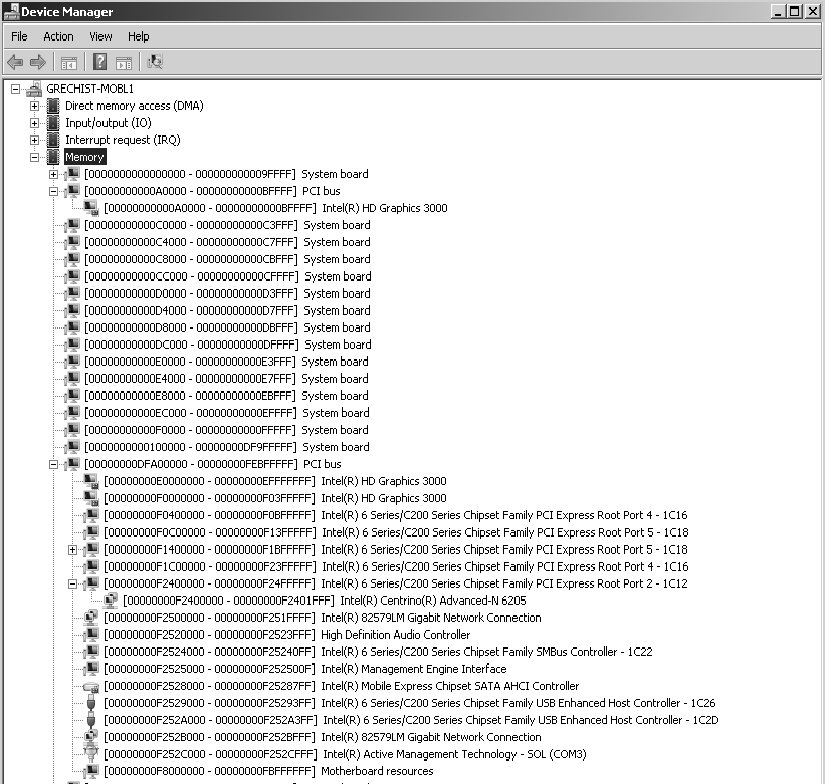
\includegraphics[width=0.9\textwidth]{./memmap-device-manager}
    \caption[Выделение диапазонов памяти в~Windows]{Выделение диапазонов памяти под нужды периферийных устройств в~Windows, наблюдаемое через диспетчер устройств}
    \label{fig:memmap-device-manager}
\end{figure}


\subsection[Карты пространств памяти]{Карты пространств памяти (memory space mappings)}\label{sec:mem-maps}

В реальных сценариях работы функционирование пространств памяти может усложняться следующими обстоятельствами.

\begin{itemize*}
\item Состояние устройств в пространствах памяти может меняться со временем согласно внутренним принципам процесса загрузки системы; количество их регистров также подвержены изменению, их адреса в памяти — тоже.
\item Несколько устройств могут быть расположены в пересекающихся диапазонах адресов, требуя динамического разрешения конфликтов.
\item Одно и то же устройство может одновременно быть расположено по нескольким диапазонам адресов и при этом обеспечивать в них различные побочные эффекты.
\end{itemize*}

Для учёта всех этих особенностей в симуляции используется такая структура, как карта памяти. Для любого доступа по адресу в памяти алгоритм определения устройства, отвечающего за его обработку, следующий~\cite{simics-model-builder-guide} (рис.~\ref{fig:mapalg}).

\begin{figure}[htb]
    \centering
	\inputpicture{drawings/mapalg}
    \caption[Алгоритм поиска устройства в иерархии карт памяти]{Алгоритм поиска устройства в иерархии карт памяти. Перед передачей транзакции доступа конечному устройству её параметры, например адрес, могут быть изменены}
    \label{fig:mapalg}
\end{figure}

\begin{enumerate*}
\item Для доступа определяется его тип (чтение, запись, предвыборка, чтение инструкции и т.п.), адрес начала, длина доступа.
\item В карте памяти по адресу начала определяется нижележащее устройство, которое, в свою очередь, может быть или конечным устройством, или ещё одной картой памяти.
\item Если ни одно устройство не имеет записи в карте, используется устройство по умолчанию (\abbr default target), если оно определено для текущей карты.
\item При необходимости параметры доступа модифицируются так, чтобы соответствовать устройству, например адрес смещается на фиксированную величину.
\item Если полученное устройство — карта памяти, то поиск продолжается в ней, иначе доступ в память передаётся найденному устройству на обработку. 
\item Ситуация, когда для данного адреса не существует трансляции, является ошибкой в конфигурации модели. Также, скорее всего (но необязательно), по конвенциям работы аппаратуры и исполняющейся программы некорректным будет являться многобайтный доступ, части которого попадают в различные устройства.
\end{enumerate*}

Для разрешения неоднозначности при ситуации, когда одно и то же устройство размещено в нескольких картах, в доступе в память из карты добавляется дополнительное число — номер функции. При обработке транзакции устройство может проверить данный номер и скорректировать своё исполнение. Ещё одна задача, которую выполняют с помощью карт памяти — динамическое изменение порядка байт (endianness) доступа, если конечное устройство это требует.

\section{Линии прерываний}

Прерывания являются ещё одним методом коммуникации пери\-фе\-рий\-ных устройств, чаще всего с ЦПУ. Однако, в отличие от рассмотренных ранее способов, оно характеризуется следующими отличиями.

\begin{itemize*}
\item Инициатором взаимодействия является периферийное  уст\-ройст\-во. Процессор в зависимости от ряда условий может отложить обработку полученных прерываний до момента, когда это станет возможным или алгоритмически корректным, или же немедленно перейти в процедуру обработки.

\item Прерывание несёт один бит информации, означающий, что на каком-то из внешних устройств имеется событие, требующее внимания. На каждую линию может быть подключено несколько устройств; в таком случае получатель сигнала прерывания не способен сразу различить, которое из них было инициатором — требуется проинспектировать все из них.

\item Коммуникации однонаправленны в отличие от, например, чтения из регистра, при котором как читающее, так и пишушее устройство имеет возможность получить некоторую информацию о взаимодействии.
\end{itemize*}

% However, it is always treated separately for a number of reasons. It is device-initiated, as opposed to the methods mentioned above, which are CPU-initiated. It is also unidirectional, as information flows only from device to CPU. Lastly, each interrupt line carries only one bit of information with a fixed meaning, namely "an event that requires attention has occurred in a device on this interrupt line".

%Моделирование работы линии прерываний сильно зависит от её архитектурных особенностей. В общем случае оно может быть реализовано как обратный вызов (\abbr callback).

Моделирование работы линии прерываний может быть выполнено следующим способом: в модели архитектурного состояния устройства-получателя заводится флаг \texttt{bool interrupt_raised}, обозначающий, что произошло прерывание. Процессор после каждой исполненной инструкции проверяет состояние этого флага и в случае, когда он выставлен, меняет своё состояние соответствующим образом, при этом сбрасывая флаг в начальное положение. Недостатки данного подхода: 1) обнаружение события прерывания сдвигается на границу между исполнением инструкций, \emph{после} текущей, что не всегда корректно — некоторые прерывания могут отменять текущую инструкцию, не допуская завершения её симуляции; 2) частый опрос флага снижает скорость работы модели. Альтернативный подход: использовать обратный вызов (\abbr callback) — указатель на функцию (метод), непосредственно оперирующий состянием процессора. Инициатор прерывания имеет возможность вызвать указанную функцию для сигнализации прерывания, и затем уже логика работы самого процессора должна определять, в какой момент оно будет им обработано.

\section{Оптимизации при моделировании}

Как было описано выше, достаточно просто обеспечить моделирование состояния с помощью переменных и массивов переменных, хранящихся в памяти. Такое решение универсально и используется во всех случаях. Тем не менее для ускорения работы моделей иногда применимы описанные далее оптимизации.

\subsection{Прямое использование состояния хозяина}

В ряде ситуаций хозяйское оборудование предоставляет аппаратные ресурсы, в том числе и регистры, которые можно переиспользовать для нужд модели, одновременно ускоряя её. Состояние гостевой системы (частично) хранится не в медленной оперативной памяти, а в более быстрых регистрах.

Такой режим работы модели приобретает признаки прямого исполнения. Цикл симуляции при этом имеет следующие стадии.

\begin{itemize*}
\item Гостевое состояние регистров/памяти загружается на соответствующие регистры хозяина.
\item Симуляция проводится в течение некоторого времени.
\item При восстановлении контекста хозяина гостевое состояние сохраняется во внешнюю память.
\end{itemize*}

Как и во всех случаях использования прямого исполнения, выигрыш от него нивелируется необходимостью переключения контекста хозяина и гостя, и поэтому перед его реализацией следует оценить, будет ли польза от достаточно кропотливой работы по включению подобной функциональности в модель. Кроме того, применимость метода сильно зависит от степени соответствия архитектур хозяина и гостя.

\subsection{Кэширование доступов к картам памяти}

Как было показано в п. \ref{sec:mem-maps}, обращение по адресу к физической памяти подразумевает инспектирование одной или более карт для определения адресата. Эта процедура может быть длительной и замедлять моделирование исполняющих устройств. Возможность оптимизации здесь проистекает из наблюдения, что подавляющая часть архитектурных запросов в память оканчиваются в ОЗУ-подобных устройствах, не предоставляющих побочных эффектов. Поэтому сам факт обращения к карте памяти можно отложить или скомбинировать с последующими запросами с помощью кэширования на стороне запрашивающего исполняющего устройства, что позволит ему проводить агрессивные оптимизации своей работы.

Подобная техника должна аккуратно отслеживать изменения в используемых картах памяти. Так, при смене типа устройства, обслуживающего некоторый диапазон пространства адресов, все агенты, имевшие возможность кэшировать его, должны быть уведомлены об этом для обеспечения корректной работы модели.

\subsection{Ленивое вычисление флагов}

Один из типов регистров, встречающихся в современных процессорах — это регистр флагов, каждый бит которого означает, что результат предыдущей операции (как правило, арифметической или логической) имеет определённые свойства. Так, флаг ZF (\abbr zero flag) выставляется в значение 1, если результат предыдущей команды равен нулю, OV (\abbr overflow flag) — если он не может быть сохранён в ограниченном числе двоичных разрядов, отведённых для него, и т.д~\cite{intelmanual1}. Корректное моделирование очень большого числа инструкций подразумевает вычисление и сохранение отдельных битов регистра флагов. Даже для простой операции сложения, результат которой получается с помощью единственной машинной инструкции хозяина, приходится включать длинный блок в десятки инструкций для проверки свойств данного результата.

Общим наблюдением, ведущим к идее следующей оптимизации, является тот факт, что результат, хранящийся в регистре флагов, используется далеко не каждой последующей инструкцией, и потому нет нужды обновлять его так часто. Достаточно производить такую работу только когда это действительно будет необходимо для корректной обработки операции, зависящей от регистра флагов~\cite{bochs}, или при инспектировании состояния пользователем. 

\begin{digression}
В программировании подход (стратегия) вычислений, при котором анализ и исполнение выражения происходит лишь при необходимости использовать его результат, называется \textit{ленивым} (\abbr lazy), в отличие от \textit{энергичного} (\abbr eager) подхода, при котором выражение вычисляется сразу после доступности значений всех его входных слагаемых. % Ленивые вычисления позволяют 
\end{digression}

\section{Точки сохранения}

Возможность сохранения состояния программы в файл с возможностью последующего восстановления и возобновлением работы из него является необходимым для широкого класса приложений: параллельные программы, отказоустойчивые системы, энергосберегающие программы. Для симуляторов наличие такой функциональности означает экономию времени при изучении поведения гостевых систем. Рассмотрим, что должно входить в такую \textit{точку сохранения} (\abbr checkpoint или savepoint).

\begin{itemize*}
    \item Архитектурное состояние всех моделируемых устройств. Если использовались некоторые из описанных выше техник увеличения скорости симуляции, например, размещение состояния на хозяйских регистрах, то необходимо предварительно привести модель в <<стабильный>> режим, когда все подлежащие сохранению регистры имеют гарантированное расположение в памяти.
    
\item    Если часть элементов архитектурного состояния функционально связана с другими элементами, то возможно исключить их из содержимого точки сохранения и пересоздавать их при восстановлении. Это поможет избежать возможности рассинхронизации таких элементов. Состояние программы, не определяющее архитектурное состояние моделей, как правило, не стоит сохранять — это сэкономит время на отладку. К примеру, не стоит дорожить кэшем двоичной трансляции.
    
    \item Информация о соединении моделей отдельных устройств друг с другом. Для различения объектов необходимо использовать некоторые идентификаторы, которые можно будет использовать в качестве ссылок на них в других устройствах при хранении. Такие идентификаторы должны <<переживать>> уничтожение самих объектов с их последующим пересозданием. Поэтому, например, машинные адреса не подходят, так как при перезапуске они каждый раз будут различаться.
\end{itemize*}

\subsection{Переносимость точек сохранения}

Если симулятор планируется использовать на различных хозяйских системах, то необходимо предусмотреть сценарий сохранения гостевого состояния на одной, а восстановление — на другой, и что edianness, разрядность и форматы хранения данных при этом могут различаться. Например, нельзя хранить указатели, так как на другой системе они будут бесполезны.

\subsection[Обращение во времени]{Обращённое во времени исполнение}\label{revexec}

Периодическое сохранение состояния симулируемой системы в сочетании с детерминизмом симулятора позволяет реализовать такой невозможный в реальном мире сценарий исполнения, как обращённое во времени исполнение (\abbr reverse execution), см.~рис.~\ref{fig:reverse-execution}. 

\begin{figure}[htb]
    \centering
	\inputpicture{drawings/reverse-execution}
    \caption{Обращённое во времени исполнение}
    \label{fig:reverse-execution}
\end{figure}

При периоде снятия точек сохранений $T$, текущем времени симуляции $t$  и необходимости откатиться на $\Delta t$ секунд выполняются следующие шаги.

\begin{enumerate*}
    \item Восстановление к точке $t^\star$, ближайшей слева к моменту $t-\Delta t$:
    $$ t^\star = \lfloor (t - \Delta t) / T \rfloor \cdot T. $$
    \item Прямая симуляция до необходимой точки в течение $t_{direct}$:
    $$t_{direct} = t - \Delta t - t^\star .$$
\end{enumerate*}

Поскольку любая симуляция из фиксированного состояния всегда приводит к одинаковому финальному состоянию, то указанная последовательность действий эквивалентна <<скачку>> из момента $t$ в момент $t - \Delta t$.

Постепенно увеличивая значения $\Delta t$, можно создать видимость того, что состояние модели эволюционирует в обратном направлении в симулируемом времени. 

Скорость обращённой симуляции будет обратно линейно зависеть от значения $T$ — чем чаще делаются точки сохранения, тем в среднем короче длина необходимой прямой симуляции. Однако объём памяти, требуемый для хранения всех точек сохранения, также растёт с уменьшением $T$.

\subsection{Миграция}

Процесс возобновления симуляции гостя на хозяйской системе, отличной от той, на которой была создана точка сохранения, получил название <<миграция>>. Возможность миграции важна для распределённых систем виртуализации, призванных обеспечить устойчивость исполнения и минимальный простой виртуальных машин при угрозах отказа аппаратуры физических компьютеров. Если некоторая хозяйская система сигнализирует о сбое из-за отказа жёстких дисков, памяти, питания и т.п., то виртуальные машины, исполнявшиеся до этого на ней, перезапускаются из точек сохранения, регулярно создаваемых и сохраняемых на внешнем хранилище, на оставшихся исправных хозяевах. Наблюдаемое клиентами время простоя сервиса, обеспечиваемого мигрированными виртуальными машинами, минимально.

\subsection[Формат точек сохранения]{Формат файлов точек сохранения}

Не существуют общепринятого соглашения о формате файлов, используемых для сохранения состояния гостевых систем, так как они очень сильно зависят от структуры моделей и особенностей симулятора. Сформулируем некоторые общие принципы их дизайна.

\begin{itemize*}
    \item Файлы могут быть как двоичные, так и текстовые. Хотя первый формат может обеспечить в среднем меньший размер файлов, содержимое его будет нечитаемым для человека, что усложняет отладку симулятора, разработку инструментов для обработки точек. С другой стороны, некоторые данные изначально неудобны для анализа человеком, например, содержимое памяти, дисков и других массивов данных, тогда как представление их в текстовом виде сильно раздувает их объём. Такие данные следует хранить в двоичном виде, а оставшиеся текстовые данные могут быть сжаты архиватором.
    \item Следует предусмотреть возможность использования общепринятых стандартов хранения данных при проектировании нового формата точек сохранения, т.е. не следует <<изобретать велосипед>>. Например, для представления иерархических данных можно использовать XML (\abbr extended markup languange) или JSON. Для хранения однородных массивов данных, используемых для представления состояния жёстких дисков, оперативной памяти и т.п. сущностей существуют форматы QCOW2 или VMDK. Такой шаг повысит удобство конвертации в/из сторонних смуляторов.
    \item Необходимо явно прописывать endianness сохраняемых данных для выбранного формата. Это поможет в дальнейшем при адаптации симулятора для новых гостевых и хозяйских систем.
\end{itemize*}

\subsection{Инкрементальные точки сохранения}

В ситуациях, когда несколько точек сохранения создаются последовательно с некоторым интервалом для одной симуляции, первая из них должна полностью описывать состяние системы, а последующие точки могут опускать часть данных, не изменившихся с предыдущего раза, и содержать только <<дельту>>,  а также ссылку на предыдущую точку. Это позволяет экономить хозяйское дисковое пространство. Особенно сильный выигрыш происходит при хранении образов дисков и памяти.



\section{\Questions к главе \ref{state}} %\label{state-questions}

\subsection*{Вариант 1}

\begin{questions}

\question[3] Какой байт будет расположен первым в памяти на Little Endian системе при записи числа \texttt{0xaabbccdd} в память?
\begin{solution}[1cm]
0xdd
\end{solution}

\question[3] Выберите правильное отношение для фразы <<машинное слово длиной $w$ байт выровнено в памяти по адресу $addr$>>:
\begin{choices}
    \choice $addr \neq 0\ (\mod w)$ (адрес не делится нацело на длину слова),
    \choice $w = 2^k$ и $addr = 2^m$, $k,m \in \mathbb{N}$ (адрес и длина являются степенями двойки),
    \choice $w = 2^k$ и $addr = 2^m$, $k \leq m $ ,$k,m \in \mathbb{N}$ (адрес и длина являются степенями двойки, степень длины меньше степени адреса),
    \correctchoice $addr = 0\ (\mod w)$ (адрес делится нацело на длину слова).
\end{choices}

\question[3] Почему симулятор не имеет права кэшировать регионы гостевой памяти, помеченные как отображённые на устройства?
\begin{solution}[2cm]
В отличие от простой памяти, хранящей данные без изменений, устройство может менять своё состояние и соответственно содержимое регионов памяти на каждом доступе к нему.
\end{solution}

\question[3] Определение понятия <<машинное слово>>.
\begin{solution}[1cm]
Максимальный объём данных, который процессор данной архитектуры способен обработать за одну инструкцию. 
\end{solution}

\question[3] Какой интегральный тип языка Си наиболее удачно использовать для хранения состояния моделируемого регистра шириной 32 бита?
\begin{choices}
    \choice \texttt{int},
    \choice \texttt{unsigned int},
    \correctchoice \texttt{uint32_t},
    \choice зависит от хозяйской системы.
\end{choices}

\end{questions}

\subsection*{Вариант 2}

\begin{questions}

\question[3] Какой байт будет расположен первым в памяти на Big Endian системе при записи числа \texttt{0xbaadc0de} в память?
\begin{solution}[1cm]
0xba
\end{solution}


\question[3] Какую стратегию подразумевает концепция ленивого вычисления?
\begin{choices}
    \choice Замена точного значения выражения приближённым, но получаемым за меньшее время.
    \correctchoice Запуск вычисления выражения происходит лишь при необходимости использовать его результат.
    \choice Выражение вычисляется сразу после доступности значений всех его входных слагаемых.
    \choice Значение подвыражения, используемого в нескольких других выражениях, сохраняется при первом вычислении и затем переиспользуется.
\end{choices}

\question[3] Определение понятия <<байт>>.
\begin{solution}[1cm]
Минимальная адресуемая в данной архитектуре единица информации.
\end{solution}

\question[3] Сколько бит информации получает процессор при первоначальном возникновении сигнала на линии прерывания?
\begin{choices}
    \correctchoice 1 бит.
    \choice 8 бит.
    \choice Зависит от архитектуры.
\end{choices}

\question[3] Выберите правильные окончания фразы: карта памяти
\begin{choices}
    \correctchoice использует цель по умолчанию, если обрабатываемый запрос не попадает ни в одно из устройств,
    \choice может указывать на устройство не более одного раза,
    \choice должна указывать на все присутствующие в гостевой системе устройства,
    \correctchoice может указывать не только на устройства, но и на другие карты памяти.
\end{choices}


\end{questions}

% К каждой лекции должно быть от 8 до 12 задач, у каждой задачи должно быть 3-5 вариантов формулировок примерно одинаковой сложности. Допускается объединение нескольких последовательных лекций в одну тему и подготовка тестов к темам.
% Задачи должны полностью соответствовать материалам лекций, то есть лекциях должно быть достаточно информации для ответа на все вопросы.
% Формулировка каждого варианта задачи должна содержать всю необходимую информацию и не должна ссылаться на тексты внутри лекции, картинки или другие задачи или варианты задачи.
% Правильные ответы выделяются знаком «+» перед их формулировкой. Правильных ответов может быть несколько. Для тестов с несколькими ответами как минимум один ответ должен быть правильным и как минимум один ответ должен быть неправильным. 
% 
% Структура теста к лекции
% 
% \subsection*{Задача 1}
% 
% \paragraph{Вариант 1} 
% 
%     Чему равно 2+2?
%         Ответ 1. 3
%         + Ответ 2. 4
%         …
%         Ответ N. 5
% \paragraph{Вариант 2}
%     Чему равно 2*2?
%         + Ответ 1. 4
%         + Ответ 2. 2+2
%         …
%         Ответ N. 5
% \paragraph{Вариант 3}
% 
%     Чему равно 2-2?
%         Ответ 1. 0
% 
% 
%         
% \section{Просто подборка вопросов}
% 


 
 
 
\iftoggle{webpaper}{
    \printbibliography[title={Литература}]
}{}




\chapter{Сверхоперативная память --- кэши}\label{caches}

\dictum[Дональд Кнут. Искусство программирования. Сортировка и поиск]{Эта глава могла бы носить более претенциозное название --- <<Хранение и получение информации>>; с другой стороны, её можно было бы назвать кратко и просто --- <<Просмотр таблиц>>.}

\section{Стена памяти}

С развитием технологии микропроцессоры становились всё быстрее за счёт повышения тактовой частоты, увеличения ширины машинного слова и других факторов. В определённый момент было замечено, что все эти улучшения не дают существенного прироста скорости исполнения программ по той причине, что рост скорости оперативной памяти, используемой в ЭВМ, не столь стремителен. В результате процессор вынужден простаивать, ожидая, пока данные из памяти будут доставлены. Данная проблема получила название \textit{стены памяти} (\abbr memory wall, рис.~\ref{fig:mem-wall}) и означает, что в случае неизменности основных принципов организации вычислений рост производительности систем будущего ограничен именно скоростью оперативной памяти. 


\begin{figure}[htb]
    \centering
	\inputpicture{drawings/mem-wall}
    \caption[Сравнение темпов роста скоростей памяти и ЦПУ]{Сравнение темпов роста скоростей оперативной памяти (DRAM) и микропроцессоров (CPU)}
    \label{fig:mem-wall}
\end{figure}

\section{Назначение, принцип работы}

Существует как минимум две области применения сверхоперативной памяти. Первая из них связана с описанной выше проблемой медленности доступа к ОЗУ. Вторая --- с обеспечением корректной и быстрой синхронизации работы многопроцессорных систем.

\subsection{Ускорение обращений в память}

Частично компенсировать данную проблему призваны устройства сверхоперативной памяти, в настоящее время чаще всего именуемые \textit{кэшами} (\abbr cache). Для большинства алгоритмов наблюдается выполнение принципов как \textit{временн\'ой}, так  и \textit{пространственной}  локальности: данные, к которым обращались недавно, скорее всего, будут запрошены снова в ближайшем будущем; кроме того, вероятно, что соседние с ними данные тоже будут запрошены (рис.~\ref{fig:locality}.). Представляется разумным иметь небольшое по сравнению с основной оперативной памятью хранилище, расположенное ближе к процессору и потому работающее быстрее, чтобы хранить в нём наиболее часто запрашиваемые данные. В кэше хранятся копии блоков информации, соответствующих подмножеству адресов оперативной памяти~\cite{ulrich-cpumemory, ulrich-cpumemory-rus}.

% Benchmark: splash2x.fft from PARSEC 3.0
% Environment: Simics 4.8 stall mode, viper, ubuntu 12.04 x86_64, tracer for data only
% Period: 100 000 000 instructions , > 40 M accesses.
% 
\begin{figure}[htb]
    \centering
    \inputpicture{drawings/locality}
    \caption[Пример явлений временн\'ой и пространственной локальности]{Пример явлений временной и пространственной локальности доступов памяти при работе приложения. На графике показаны первые 5000 доступов к данным в памяти для программы \texttt{splash2x.fft} из набора PARSEC 3.0~\cite{parsec}, скомпилированной для Ubuntu 12.04 x86_64}
    \label{fig:locality}
\end{figure}

Данные в кэш попадают двумя способами. Во-первых, новый регион памяти может быть запрошен впервые за время работы, причем его придётся извлекать из основной памяти с задержкой, однако копия попадёт в кэш, и последующие обращения будут обработаны быстрее. Во-вторых, программист может предусмотреть, что некоторый диапазон памяти вскоре будет использован, и использовать явную \textit{предварительную загрузку} (\abbr prefetching) ещё до первого к нему обращения. Многие архитектуры имеют для этого специальные инструкции.

Поскольку ёмкость кэша невелика, а рабочее множество программы со временем меняется, неизбежно возникает ситуация, когда часть кэша придётся использовать для новых данных, а хранившийся там блок или отбросить, или, если он был изменён, записать обратно в память. Такой процесс называется \textit{вытеснение} (\abbr eviction).

Случаются ситуации, когда содержимое всего кэша перестаёт быть релевантным исполняемому коду. В таком случае происходит \textit{сброс} (\abbr flush) кэша, когда из него принудительно вытесняются все данные.

\subsection{Поддержка транзакций}
% \paragraph{Поддержка транзакций}

Использование дополнительного буфера в виде кэша позволяет откладывать момент записи в память, накопляя в нём совершённые последовательные изменения, применённые к различным адресам в памяти. Затем содержимое может быть записано за один раз, создавая видимость неделимости (атомарности) акта модификации ---  для внешнего наблюдателя памяти это будет выглядеть так, как будто сразу, без промежуточного состояния, изменилось большое число байт. Мы получаем транзакционную семантику записей в память. С другой стороны, если по каким-то причинам было решено, что все доступы в память, содержащиеся в кэше некоторого процессора, уже неактуальны, можно просто очистить его --- откатить транзакцию, и для внешнего наблюдателя это будет выглядеть так, как будто никаких операций над памятью не было выполнено.

Описанный  механизм является основным для реализации т.н. систем с аппаратной \textit{транзакционной памятью}~\cite{rajwar2002}.

\begin{digression}

Акцент данной главы смещён от собственно сценариев/алгоритмов эмуляции к описанию архитектурных принципов работы самой сверхоперативной памяти. 

Первый сценарий применения систем кэшей подразумевает улучшение временных характеристик основного оперативного запоминающего устройства прозрачно для исполняющихся программ. Во многих функциональных моделях, пренебрегающих задержками, модели кэша может и не быть вовсе, несмотря на то, что в реальной аппаратуре он присутствует. Необходимость в его аккуратном моделировании возникает при  исследовании производительности подсистемы памяти.

Во втором случае влияние кэшей видимо на функциональном уровне и уже нельзя пренебрегать их функциональным моделированием. В наборе инструкций могут присутствовать команды управления транзакциями. Примером является расширение Intel\textregistered TSX~\cite[глава 8]{intel-x-reference}, появившееся в процессорах микроархитектуры Haswell.

\end{digression}


\section{Устройство кэша --- линии, тэги, ассоциативность}

Рассмотрим общий принцип организации кэша\footnote{Следует отметить, что описываемая схема не является единственно возможной. Интересующийся читатель найдёт более полную картину в \cite{hennessy-patterson}.}. См. рис.~\ref{fig:cache}.

% TODO rewrite the figure using bytefield package facilities
\begin{figure}[htb]
    \centering
	\inputpicture{drawings/cache}
    \caption[Организация кэша в линии, сеты, пути]{Организация кэша в линии, сеты $N_{sets}$, пути $N_{ways}$. Ячейка содержит информацию: тэг, флаги и собственно данные линии}
    \label{fig:cache}
\end{figure}


Единица хранимых данных именуется \textit{линией кэша}. Как правило, она имеет ёмкость в несколько машинных слов и хранит копию последовательной области памяти, начиная с адреса, выровненного по размеру линии. В современных процессорах размер линии может быть 32 или 64 байта. 

Смысл кэша состоит в возможности быстрого нахождения соответствия «адрес--данные» (ситуация \textit{попадания в кэш}, \abbr cache hit) или констатации отсутствия такого соответствия (ситуация \textit{промаха}, \abbr cache miss). Алгоритм такого поиска состоит из следующих шагов.

\begin{enumerate*}
\item Каждая ячейка кэша кроме собственно копии данных содержит вспомогательную информацию, состоящую из тэга и группы флагов.

\item Из адреса в памяти выделяются смещение байта внутри линии \textit{offset}, номер множества (сета) $n_{set}$ и тэг $tag$. Пример такого разбиения приведён на рис.~\ref{fig:set-tag-flags}. Алгоритм выделения $n_{set}$ и $tag$ может быть произвольным, однако он должен позволять однозначно идентифицировать адрес линии.

\begin{figure}[htb]
    \centering
	\inputpicture{drawings/set-tag-flags}
    \caption[Пример выделения значений номера сета, тэга и смещения из адреса]{Пример выделения значений номера сета, тэга и смещения по диапазонам бит из адреса в шестнадцатеричном представлении}
    \label{fig:set-tag-flags}
\end{figure}


\item Выбирается сет с указанным $n_{set}$. Искомая линия может находиться в любом из $N_{ways}$ позиций в нём; ищется ячейка, содержащая тэг, равный $tag$. Аппаратная реализация большинства кэшей подразумевает, что поиск этот происходит параллельно во всех линиях сета и потому занимает фиксированное время.

\item Если удовлетворяющая условию ячейка найдена, проверяется, активна ли она или является «мусором», оставшимся от предыдущей работы.

\item В случае нахождения тэга и валидности мы имеем попадание в кэш, иначе же --- промах.
\end{enumerate*}

Таким образом, следующие параметры определяют описанный выше простой кэш.

\begin{itemize*}
\item Ёмкость линии данных $S_{line}$, измеряемая в байтах.
\item    Ассоциативность $N_{ways}$ определяет, сколькими способами одна и та же линия может быть размещена в ячейках кэша,  а также адреса линий, конкурирующих с ней за место (очевидно, что линии с разным значением $n_{set}$ всегда будут в разных сетах и не могут вытеснять друг друга). Если $N_{ways} = 1$, то мы имеем кэш \textit{прямого отображения} (\abbr directly mapped cache), в котором линия с определённым адресом, если она присутствует, всегда занимает одну и ту же ячейку. Соответственно, если $N_{sets} =1$, мы имеем полностью \textit{ассоциативный кэш} (\abbr fully associative cache), в котором линия может занимать любую ячейку.

\item    Количество сетов $N_{sets}$ должно быть достаточно большим, чтобы вместе с ёмкостью тэга быть способным полностью адресовать все возможные адреса линий в памяти системы. В противном случае некоторые диапазоны памяти просто не смогут быть отображены на ячейки.

\item    Ёмкость кэша --- $C$. Очевидно, что она равна произведению рассмотренных ранее величин:

$$C = S_{line}N_{ways} N_{sets}.$$
\end{itemize*}


\section{Промахи. Алгоритмы вытеснения линий}

Что должно происходить, если был детектирован промах кэша? Отсутствующие данные запрашиваются из памяти и, как правило, после получения помещаются в кэш. Для размещения новой линии может быть использована любая пустая, т.е. не содержащая актуальных данных, ячейка.

Как поступать, если все ячейки сета содержат актуальные данные? В таком случае выбирается одна из них, и её содержимое вытесняется и заменяется на новое. Перед этим проверяется ещё один флаг --- \textit{модификации} (\abbr dirty), поднимаемый при первой записи в ячейку. Если хранящиеся  в линии данные отличаются от версии, содержащейся в оперативной памяти, то необходимо передать их из кэша обратно в ОЗУ. Для ячеек, использовавшихся только для чтения, в этом нет необходимости, и они могут быть сразу перезаписаны.

Как выбрать, какую ячейку текущего сета следует вытеснить? «Идеальный» алгоритм --- выбирать линию с адресом, к которому впоследствии программа не будет обращаться дольше всего. Однако  его реализация подразумевает знание поведения алгоритма в будущем, а такой анализ в общем случае как минимум затруднителен, а с практической стороны и вовсе невозможен. Мы можем отталкиваться от истории предыдущих доступов к линиям при формулировке \textit{политики вытеснения} (\abbr replacement policy) линий.

Перечислим лишь некоторые из существующих алгоритмов~\cite{arc}.

\begin{itemize*}
\item    Вытеснять всегда первую ячейку. Очевидно, что это --- единственная доступная схема работы для кэша с прямым отображением. Для ассоциативных кэшей она нецелесообразна.

\item    Вытеснять случайную ячейку. Политика довольно проста в реализации, не требует хранения дополнительных данных для каждой ячейки, но может оказаться субоптимальной на практике.

\item    FIFO (\abbr first in first out) --- \textit{классическая очередь}. Для каждого сэта хранится порядок, в котором занимались его ячейки. Для вытеснения выбирается самая <<старая>> ячейка. Достоинство данной политики --- в простоте и небольших накладных расходах «в железе». Однако для наибольшей эффективности алгоритма необходимо, чтобы приложение, использующее память, имело потоковый характер чтения памяти, что далеко не всегда наблюдается на практике --- к некоторым ранее затребованным адресам оно может обращаться снова и снова с нерегулярными интервалами.

\item    LRU (\abbr least recently used). Для каждой ячейки хранится её «возраст» --- величина, пропорциональная времени, прошедшему с момента последнего к ней обращения. При вытеснении выбирается самая «старая» ячейка, т.к. к ней не обращались дольше всего и потому, возможно, не обратятся в ближайшем будущем. Данная политика (и её различные оптимизации) является самой популярной из-за наилучшего сочетания точности работы и сложности реализации.

\end{itemize*}

\section{Трансляция адресов и кэш}

В большинстве современных архитектур процессоры имеют поддержку виртуальной (в русской традиции называемой \textit{математической}) памяти для многозадачных режимов работы. При этом каждая программа, исполняющаяся на машине, видит собственное упрощённое адресное пространство, содержащее код и данные только её самой, и использует его вне зависимости от местоположения в физической, «настоящей» памяти. 

Поиск в кэше может происходить по физическому адресу, по виртуальному или даже по их комбинации. Схема разбиения адресов на тэг и номер сета может быть различная, но подразумевающая однозначное соответствие линий в памяти и ячеек кэша\footnote{В этой и последующих секциях данной главы часть текста по архитектуре кэшей адаптирована из русского и английского разделов Википедии: \url{http://ru.wikipedia.org/wiki/Кэш_процессора}.}.

Наличие виртуальной памяти требует от процессора проведения трансляции виртуальных  адресов, используемых программой, в физические адреса, соответствующие реальному местоположению в ОЗУ. При этом возникают следующие обстоятельства.

\begin{itemize*}
\item    \textit{Задержка.} Значение физического адреса будет готово только спустя некоторое время (несколько тактов) после запроса преобразования виртуального. Потому при обращении к кэшу только по физическим адресам мы будем вынуждены ожидать завершения процесса преобразования, если не используется специальное устройство для кэширования отображений виртуальных адресов --- буфер ассоциативной трансляции (\abbr TLB, translation look-aside buffer).

\item    \textit{Эффект наложения.} Несколько виртуальных адресов могут соответствовать одному физическому (\abbr aliasing). Поэтому требуется проверка, что только одна линия с данным физическим адресом находится в кэше в любой момент времени.
\end{itemize*}

По использованию виртуальной адресации кэши могут быть классифицированы следующим образом. 
\begin{enumerate*}
\item Physically indexed, physically tagged (PIPT) --- \textit{физически индексируемые и физически тегируемые}. Они просты и избегают проблем с наложением, но медленны, так как перед обращением в кэш требуется запрос физического адреса в TLB. Этот запрос может вызвать промах в TLB и дополнительное обращение в основную память перед тем как наличие данных будет проверено в кэше.

\item Virtually indexed, virtually tagged (VIVT) --- \textit{виртуально индексируемые и виртуально тегируемые.} И для тегирования, и для индекса используется виртуальный адрес, благодаря чему проверки наличия данных в кэше происходят быстрее, не требуя использования трансляции. Однако возникает проблема наложения, когда несколько виртуальных адресов соответствуют одному и тому же физическому. В этом случае данные будут дважды помещены в разные ячейки, что усложняет поддержку когерентности. Другой проблемой являются \textit{гомонимы} (\abbr homonyms)---  ситуации, когда в один и тот же виртуальный адрес (из разных пользовательских процессов) отображаются различные физические адреса. Невозможно различить их исключительно по виртуальному индексу. Возможные решения: сброс кэша при переключении между задачами (context switch), требование непересечения адресных пространств отдельных процессов, тегирование виртуальных адресов идентификатором адресного пространства, использование физических тегов.

\item Virtually indexed, physically tagged (VIPT) --- \textit{виртуально индексируемые и физически тегируемые.} Для индекса используется виртуальный адрес, а для тега --- физический. Преимуществом над первым типом является меньшая задержка, поскольку можно искать кэш-линию одновременно с трансляцией адресов в TLB, однако сравнение тега всё равно задерживается до момента получения физического адреса. Преимуществом над вторым типом является безопасное обнаружение гомонимов, так как тег содержит физический адрес. Для данного типа требуется выделять больше бит для хранения тега, поскольку индексные биты используют иной тип адресации.

\item Physically indexed, virtually tagged --- \textit{физически индексируемые и виртуально тегируемые}. Такие кэши не дают существенных преимуществ и в настоящее время представляют исключительно академический интерес.
\end{enumerate*}

\section{Иерархии кэшей}

\subsection{Многоуровневые системы}

Может показаться очевидным, что чем больше ёмкость установленного кэша, тем эффективнее будет работать подсистема памяти из-за меньшей частоты промахов, необходимости вытеснения линий в ассоциативных сетах. Однако на практике эта величина ограничена многими факторами, в первую очередь доступной площадью на кристалле и энерговыделением. Кроме того, увеличение количества линий ведёт к росту геометрических размеров кристалла, время, затрачиваемое на передачу сигналов, растёт, нивелируя эффект от большего количества данных.

Невозможность улучшать уже присутствующие в системе устройства приводит к необходимости введения ещё одного промежуточного хранилища между ядром процессора и ОЗУ --- кэш второго уровня (L2). Он располагается сразу после кэша первого уровня (L1) и характеризуется большими задержками доступа, но при этом может иметь большую ёмкость, см. рис.~\ref{fig:l1l2}.

\begin{figure}[htb]
    \centering
	\inputpicture{drawings/l1l2}
    \caption{Иерархия памяти, состоящая из двух кэшей и ОЗУ}
    \label{fig:l1l2}
\end{figure}


Теперь при ситуации промаха в кэше первого уровня данные сначала ищутся во втором уровне, и лишь при втором промахе обращение идёт в память. 

Естественно, что иерархию памяти можно продолжать наращивать, добавляя новые, менее быстрые и более ёмкие уровни сверхоперативной памяти. %В большинстве современных процессоров имеется трёхуровневая система кэшей.

Для таких систем возникают следующие вопросы проектирования: на каких уровнях системы должна содержаться линия с определённым адресом при различных историях обращений к ней? Может ли одна линия находиться одновременно в нескольких уровнях кэша?

В одном случае могут потребовать, чтобы все данные, хранящиеся в кэше L1, находились также и в кэше L2. Такие пары кэшей называют строго \textit{инклюзивными} (\abbr inclusive). Другие процессоры могут не иметь подобного требования, тогда кэши называются \textit{эксклюзивными} (\textit{исключительными})  --- данные могут быть либо в L1, либо в L2 кэше, но никогда не могут быть одновременно в обоих.

До сих пор другим процессорам не требовалось, чтобы данные в кэше первого уровня также размещались в кэше второго уровня, тем не менее они продолжают так делать. Нет общепринятого имени для этой промежуточной политики, хотя часто используется термин \textit{инклюзивно} (\abbr mainly inclusive).

\subsection{Кэши инструкций и данных}

Инструкции, как и данные, хранятся в общем пространстве памяти\footnote{Для ЭВМ архитектуры фон Неймана; тем не менее дальнейшие рассуждения в основном применимы и для систем с гарвардской архитектурой.}; как и в случае данных, быстрый доступ к ним является необходимым условием скорости исполнения приложений. Однако множества используемых адресов и характерные шаблоны доступов для кода и данных чаще всего различны, что при их совместном кэшировании создало бы чрезмерную нагрузку и неоптимальное использование ресурсов сверх\-опера\-тивной памяти. Поэтому отдельно выделяют кэш инструкций (\abbr instruction cache, IC) и кэш данных (\abbr data cache, DC). Отметим, что в IC приходят только запросы на чтение. При работе такой системы нужно следить за тем, чтобы запись в DC по адресам линий, находящихся в IC, приводила к их сбросу\footnote{В некоторых архитектурах для этого следует явно вызывать инструкцию, в остальных происходит автоматически.}.

\section{Кэши в многопроцессорных системах}

В современных ЭВМ доступ к памяти могут одновременно иметь как несколько независимых процессоров (в многоядерных системах), так и ряд периферийных устройств (в системах с DMA --- \abbr direct memory access). Каждый из них может иметь свои приватные кэши, в которых хранятся копии линий, в том числе и локально модифицированных.  Необходимо, чтобы все агенты имели единое представление о содержимом ОЗУ. Кроме того, на производительность иерархии памяти, связанной с одним ядром, влияет то, как линии переходят между разными его уровнями.

\subsection[Классификация моделей согласованности]{Классификация моделей согласованности доступов в память}


Модель согласованности (консистентности) представляет собой некоторый договор между программами и памятью, в котором указывается, что работа модуля памяти будет корректной при соблюдении программами определённых правил. Существует их общепринятая алгоритмическая классификация~\cite{Mosberger93memoryconsistency}, основанная на различии тех моментов, когда транзакция становится видимой для сторонних наблюдателей, а также разрешённого порядка записи. Ниже перечислены лишь некоторые существующие модели.

\begin{enumerate*}
\item    \textit{Строгая согласованность.} Операция <<чтение ячейки памяти с адресом $x$>> должна возвращать значение, записанное самой последней операцией <<запись>> с адресом $x$. В системе со строгой консистентностью должно присутствовать единое абсолютное время.

\item    \textit{Последовательная согласованность} --- модель, в которой результат выполнения должен быть тот же, как если бы инструкции операторов всех процессов выполнялись в некоторой последовательности, определяемой программой для этого процессора. При параллельном выполнении все процессы должны видеть одну и ту же последовательность записей в память, то есть разрешаются запаздывания для чтения.

\item    \textit{Причинная согласованность} --- модель, не требующая, чтобы все процессы видели одну и ту же последовательность записей в память. Таким образом, проводится различие между потенциально-зависимыми (запись одной может зависеть от результата чтения другой ячейки) и потенциально-независимыми (параллельными) операциями записи.

\end{enumerate*}

На практике модели согласованности выражаются политиками записи в память, реализуемыми аппаратурой сверх- и оперативной памяти.

\subsection[Политики записи]{Политики записи: WT, WB, WC, UC}

При записи данных в кэш должен существовать определенный момент времени, когда они будут записаны в основную память, что контролируется \textit{политикой записи} (\abbr write policy). Для кэшей с политикой \textit{сквозной записи} (WT, \abbr write through) любая запись приводит к немедленной записи в память, происходящей параллельно с записью в ячейку кэша. 

Другая политика, именуемая \textit{обратной записью} (WB, \abbr write back), откладывает запись на более позднее время, которая производится при вытеснении подобной линейки из кэша. Таким образом, промах в кэше, использующем политику обратной записи, может потребовать двух операций доступа в память --- один для сброса состояния старой линейки и другой для чтения новых данных.

Режим \textit{совмещения записи} (WC, \abbr write combining) позволяет сохранять данные перед записью из кэша в память в специальном буфере, сбрасываемом за одну операцию, --- \textit{всплеск} (\abbr burst), вместо того, чтобы  писать эти линии немедленно по их прибытии, что приводит к повышению средней скорости записи. %\footnote{Фактически здесь мы видим подтверждение закона Литтла (см. главу~\ref{alternatives}).}.

Такой режим не следует использовать для доступа к «обычной» памяти кода и данных в силу её модели \textit{слабой согласованности} (\abbr weak ordering), которая не гарантирует, что последовательность записей и чтений будет выполнена в ожидаемом порядке. Например, комбинация «запись---чтение---запись» некоторого адреса при совмещённой записи выльется в последовательность «чтение---запись---запись», т.к. при чтении будет получено значение, хранящееся в памяти, а не в буфере. Для решения этой проблемы буфер может быть дополнен функциональностью полностью ассоциативного кэша --- дополнительного уровня в иерархии, что приведёт к усложнению его реализации.

Однако для видеопамяти слабая согласованность не является препятствием, и поэтому политика WC может быть использована для реализации быстрых драйверов видеокарт~\cite{wc-guidelines}.

В реальных системах различные диапазоны памяти могут иметь различные типы политик записи в память, настраиваемых с помощью атрибутов страниц ОЗУ или специальных системных регистров. В качестве одного из возможных типов может быть выбран полный \textit{запрет кэширования} (UC, \abbr uncacheable) --- такой режим необходим для регионов, соответствующих периферийным устройствам, доступ к которым вызывает немедленные побочные эффекты.

\subsection[Алгоритмы поддержания когерентности]{Алгоритмы поддержания когерентности}

Для того чтобы информация о состояниях линий в независимых кэшах соответствовала выбранной модели согласованности, используются специальные протоколы когерентности. Каждая ячейка кэша получает расширенный набор флагов, описывающий то, как её состояние соотносится с состояниями ячеек с тем же адресом, но находящихся в кэшах других агентов.

При изменении состояния некоторой линии необходимо каким-то образом сообщать о таком факте остальным кэшам. Генерируются сообщения, доставляемые по какой-либо среде внутри многопроцессорной системы (это может быть общая шина, полностью связанная сеть или сеть общего вида; сообщения могут быть адресными или широковещательными), и связанная с указанным фактом задержка влияет на скорость работы подсистемы памяти.

Было придумано много вариантов протоколов когерентности, отличающихся алгоритмами и количеством состояний, которые различаются по своей скорости работы и масштабируемости. Большинство современных протоколов представляют вариации т.н. MESI-протокола\footnote{Хороший обзор существующих протоколов с диаграммами переходов можно найти по ссылке \url{http://pg-server.csc.ncsu.edu/mediawiki/index.php/CSC/ECE_506_Spring_2011/ch8_mc}.}.

\subsubsection{MESI}

В этой схеме каждая линия имеет одно из взаимоисключающих состояний.

\begin{itemize*}
\item    \textit{Модифицированная} (\textit{M}) \abbr modified: данные в кэш-линии, помеченной как модифицированная, имеются только в одном кэше во всей системе. Линия может читаться и быть записана без опроса остальных агентов в системе.

\item    \textit{Исключительная} ( \textit{эксклюзивная} ) (\textit{E}) \abbr exclusive: кэш-линия, как и \textit{M}-линия, хранится только в одном кэше системы, однако она ещё не подверглась изменениям; данные в ней идентичны хранящимся в ОЗУ. Поскольку эксклюзивная кэш-строка хранится только в одной кэш-памяти, она может быть считана или записана без внешних запросов. После записи в линию она отмечается как модифицированная.

\item    \textit{Разделяемая} (\textit{S}) \abbr shared: линия может одновременно находиться в нес\-коль\-ких кэшах и использоваться совместно двумя или более агентами. Запросы на запись к такой линии  всегда идут на внешнюю шину данных независимо от политики записи (WT или WB) , что приводит линии в других кэшах в состояние «недействительно». При этом содержимое основной памяти также обновляется.

\item    \textit{Недействительная} (\textit{I}) \abbr invalid: линия, отмеченная как недействительная, становится логически недоступной. Это происходит в случаях, если она пуста или содержит устаревшую информацию. 

\end{itemize*}
Схема переходов представлена на рис.~\ref{fig:mesi}.

\subsubsection{MOESI}

Данный протокол является оптимизацией  обычного протокола MESI. При этом флаги состояния расширяются состоянием \textit{O} (\abbr owned), означающим, что данные в линии одновременно и модифицированы, и разделяются (modified и shared). Указанное состояние позволяет избежать необходимости записи модифицированной линии обратно в основную память, прежде чем другие процессоры системы смогут ее прочесть. Используется микропроцессорами AMD Opteron.
\begin{itemize*}
\item    \textit{Владелец} (Owned). Линия в этом состоянии содержит актуальные данные. Состояние похоже на Shared в том, что оно обозначает, что другие процессоры могут иметь копию наиболее свежих и корректных данных. Оно также обозначает, что в основной памяти данные могут быть устаревшими. Только один из агентов может иметь данную линию в состоянии Owned. В таком случае он отвечает на запросы чтения вместо медленной памяти.
\end{itemize*}

\begin{figure}[htb]
    \centering
	\inputpicture{drawings/mesi}
    \caption[Диаграмма переходов протокола MESI]{Диаграмма переходов протокола MESI. Доступ является местным, если он был инициирован процессором данного кэша, и удалённым, если запрос возник в любом другом}
    \label{fig:mesi}
\end{figure}

\subsubsection{MESIF}

Данный протокол актуален для систем с неоднородной когерентной памятью (\abbr cache coherent non-uniform memory access, ccNUMA), когда каждый процессорный сокет имеет свою, ближайшую к нему, память, а обращение к адресам других сокетов происходит через промежуточные узлы и занимает в 1,5--2 раза больше времени. Введение к протоколу MESI нового состояния \textit{F} (\abbr forward) сделано для уменьшения объёма синхронизационного траффика в таких системах; фактически \textit{F} --- это вариант \textit{S}, присутствующий ровно в одном кэше в любой момент времени.
\begin{itemize*}
\item \textit{Передовой} (\textit{F}): означает, что данный кэш является единственным выбранным ответчиком (\abbr designated responder) для любых запросов к линии с данным адресом. Остальные линии (в состоянии \textit{S}) при этом не отвечают на запросы когерентности. 
\end{itemize*}

\section{Моделирование}

При симуляции систем кэшей количество необходимых усилий напрямую зависит от реализуемой архитектуры и сценария использования этой модели.

\subsection{«Честное» моделирование}

Зачастую модель кэша повторяет устройство реальной аппаратуры очень близко для того, чтобы учесть все возможные причины возникновения задержек. При этом функционально моделируется хранение в ячейке данных, метаданных (тэги, флаги, информация для механизма вытеснения). Для иерархий кэшей учитываются передачи данных между уровнями. Для когерентных систем приходится добавлять модель среды для передачи данных и симулировать полную маршрутизацию сообщений от одних кэшей до других.

Отметим, что механизм ассоциативного поиска тэга внутри сета нереализуем программно (по крайне мере в одном потоке исполнения), и потому он заменяется более традиционными алгоритмами --- последовательный перебор, деревья, хэш-таблицы; величина задержки этой процедуры, конечно, учитывается вне зависимости от деталей модельной реализации.

\subsection{Модель задержек}

Этот подход применим в том случае, когда кэши функционально «прозрачны» и их наличие выражается только в изменении времён доступов к памяти. В таком случае мы можем упростить их моделирование,  избавившись от хранения линий --- они всегда будут лежать в устройстве памяти, кэш не будет содержать их копии. Для вычисления же времён задержек все метаданные (тэги, сеты, флаги) ячеек моделируются так же, как и в общем случае.

Для моделирования аспектов задержки доступов, связанной с необходимостью передачи данных для поддержания когерентности, может быть использована более простая схема, отражающая функциональность, но не детали её реализации; при этом время высчитывается по заранее измеренным «расстояниям» между агентами (рис.~\ref{fig:timing-model}). Такое разделение упрощает разработку модели кэшей и ускоряет исследование различных её вариантов. Однако оно неприменимо для случая моделирования транзакций, так как фактически данные никуда не перемещаются и их копии не создаются.

\begin{figure}[htb]
    \centering
	\inputpicture{drawings/timing-model}
    \caption[Раздельное моделирование функциональности и длительности доступов в~память]{Раздельное моделирование функциональности и длительности доступов в память. По указанному адресу данные возвращаются моделью памяти (кэши при этом не оказывают никакого влияния), задержки независимо вычисляются моделью кэшей}
    \label{fig:timing-model}
\end{figure}

\subsection[Влияние моделей кэшей на скорость]{Влияние моделей кэшей на скорость симуляции}

Подключение системы кэшей к функциональной модели делает её (хотя бы частично) потактовой, и естественно ожидать связанное с этим замедление симуляции. На практике скорость может упасть в тысячи раз. Поэтому часто модели кэши делают динамически отсоединяемыми от иерархии памяти, и они подключены лишь на период симуляции, когда исполняется изучаемое приложение, чтобы не тормозить предваряющие этапы загрузки операционной системы. 

Однако очевидно, что эффективность кэша будет зависеть от того, заполнен ли он актуальными данными или же пуст; во втором случае многие ранние доступы будут промахами. Поэтому после подключения некоторое время тратится на \textit{разогрев} (\abbr warm up) системы, причем статистика и задержки игнорируются (рис.~\ref{fig:warm-up}). Длительность этого процесса зависит от ёмкости кэшей и интенсивности обращений приложения к памяти; как минимум длина его не должна быть меньше длины периода измерения. Лишь после разогрева появляются основания полагать, что измеряемые на модели результаты производительности будут адекватны реальности. 

\begin{figure}[htb]
    \centering
	\inputpicture{drawings/warm-up}
    \caption[Разогрев кэшей]{<<Разогрев>> кэшей. Этап симуляции загрузки ОС проводится с помощью быстрой функциональной модели. Затем некоторое время система кэшей подключена и обрабатывает запросы, но статистика и сообщаемые ей задержки не принимаются во внимание. На последнем отрезке собираются результаты моделирования}
    \label{fig:warm-up}
\end{figure}

\section{\Questions к главе \ref{caches}} %\label{caches-questions}

\subsection*{Вариант 1}

\begin{questions}
\question[3] Выберите правильные варианты продолжения фразы: использование кэшей при работе приложения целесообразно, если
\begin{choices}
    \correctchoice    программа показывает временную локальность доступов,
    \choice программа не обращается в оперативную память,
    \choice программа работает с очень большим объёмом данных,
    \correctchoice программа показывает пространственную локальность доступов,
    \choice программа работает с объёмом данных, меньшим ёмкости кэша.
\end{choices}

\question[3] Выберите все правильные окончания фразы: функциональные симуляторы часто не содержат в себе модель кэша, потому что
\begin{choices}
    \correctchoice они влияют только на задержки, но не на семантику инструкций,
    \choice всегда имеется возможность переиспользовать хозяйский кэш для нужд симуляции,
    \correctchoice такие модели сильно замедляют симуляцию.
\end{choices}

\question[3] Данные могут попадать в кэш при следующих операциях:
\begin{choices}
    \correctchoice чтение памяти (load),
    \correctchoice запись в память (store),
    \choice арифметические операции,
    \choice операции с числами с плавающей запятой,
    \correctchoice предвыборка данных (prefetch),
    \correctchoice загрузка инструкции (fetch),
    \choice инвалидация линии (invalidate).
\end{choices}

\end{questions}

\subsection*{Вариант 2}
\begin{questions}

\question[3] Выберите правильные варианты окончания: линия данных с фикированным адресом
\begin{choices}
    \choice всегда попадает в одну и ту же ячейку кэша,
    \correctchoice всегда попадает в один и тот же сет,
    \choice может быть сохранён в любой ячейке кэша.
\end{choices}

\question[3] Выберите правильные варианты.
\begin{choices}
    \choice Темпы роста скорости оперативной памяти и процессоров одинаковы с 80-х годов ХХ века.
    \choice Темп роста скорости оперативной памяти опережает темпы роста скорости работы процессоров.
    \correctchoice Темп роста скорости процессоров опережает темпы роста скорости оперативной памяти. 
\end{choices}

\question[3] Кэши необходимо симулировать даже в функциональной модели, если они используются для
\begin{choices}
    \correctchoice создания транзакционной памяти,
    \choice моделирования работы ЭВМ гарвардской архитектуры,
    \choice поддержания когерентности в SMP системах.
\end{choices}





\end{questions}

% К каждой лекции должно быть от 8 до 12 задач, у каждой задачи должно быть 3-5 вариантов формулировок примерно одинаковой сложности. Допускается объединение нескольких последовательных лекций в одну тему и подготовка тестов к темам.
% Задачи должны полностью соответствовать материалам лекций, то есть лекциях должно быть достаточно информации для ответа на все вопросы.
% Формулировка каждого варианта задачи должна содержать всю необходимую информацию и не должна ссылаться на тексты внутри лекции, картинки или другие задачи или варианты задачи.
% Правильные ответы выделяются знаком «+» перед их формулировкой. Правильных ответов может быть несколько. Для тестов с несколькими ответами как минимум один ответ должен быть правильным и как минимум один ответ должен быть неправильным. 
% 
% Структура теста к лекции
% 
% \subsection*{Задача 1}
% 
% \paragraph{Вариант 1} 
% 
%     Чему равно 2+2?
%         Ответ 1. 3
%         + Ответ 2. 4
%         …
%         Ответ N. 5
% \paragraph{Вариант 2}
%     Чему равно 2*2?
%         + Ответ 1. 4
%         + Ответ 2. 2+2
%         …
%         Ответ N. 5
% \paragraph{Вариант 3}
% 
%     Чему равно 2-2?
%         Ответ 1. 0
% 
% 
%         
% \section{Просто подборка вопросов}
% 


 
 


\iftoggle{webpaper}{
    \printbibliography[title={Литература}]
}{}



\chapter{Языки разработки моделей и~аппаратуры}\label{lang}
\dictum[BSV by Example]{When someone comes to you with ``a new language'' it is often time to run the other way\footnotemark}
\footnotetext{Когда кто-то идёт к вам с предложением использовать <<новый язык>>, чаще всего следует развернуться и бежать в противоположном направлении.}

% Quote: Language wars are religious wars, and few of these religions are polytheistic. // Edward A. Lee "The Problem with Threads"
 
Симуляторы и входящие в их состав отдельные модели устройств сами по себе являются программами. Они пишутся на некотором выбранном языке (или нескольких языках) программирования. В законченном симуляторном решении, претендующем на право называться удобным и расширяемым, можно выделить функциональные блоки, различные по своему назначению. Пример структуры некоторого симулятора приведён на рис.~\ref{fig:breakdown}. 
% В зависимости от назначения, развитости проекта состав 
\begin{figure}[htb]
    \centering
	\inputpicture{drawings/breakdown}
    \caption[Структура и классификация компонент симулятора]{Структура и классификация компонент симулятора. Графический интерфейс и командная строка отвечают за взаимодействие с пользователем. Языки сценариев (скрипты) обеспечивают средства автоматизации и расширения функциональности. Модели устройств используются для конструирования изучаемой системы. Ядро связывает компоненты в единое целое}
    \label{fig:breakdown}
\end{figure}

Каждая из компонент симулятора может быть реализована на своём языке, наиболее адекватном требуемой функциональности. Например, графический интерфейс может быть сделан с помощью библиотек (языков) Qt (С++), AWT (Java), Tk (Tcl) и т.д. Интерпретатор сценариев, скорее всего, будет выполнен на том же динамическом языке, который предполагается использовать для написания скриптов.

Перейдём к основной части любого симулятора — моделям устройств. Для их создания можно использовать языки общего назначения, такие как Си, Си++. Их универсальность и гибкость позволит написать каждую модель «с нуля». При этом придётся самостоятельно вводить все необходимые абстракции предметной области симуляции, вычленять иерархическую структуру создаваемой системы и сопоставлять её с возможностями языка.

Однако специфика задачи моделирования такова, что является возможным выделение некоторых абстракций в законченные модули, удобные для повторного использования, и интеграции моделей, написанных разными людьми, с помощью набора документированных интерфейсов. При этом возникает возможность переиспользования части работы, уже выполненной кем-то. По этой причине в индустрии программного моделирования можно выделить два подхода.

\paragraph{Создание библиотек для языков общего назначения, реализующих необходимые для  моделирования примитивы.} В этом случае желаемые понятия формулируются в терминах типов данных, функций или объектов, полей и методов для объектно-ориентированных языков. У разработчика, использующего такую систему, остаётся полная свобода выражения, ограниченная лишь синтаксисом применяемого языка.
\paragraph{Использование специализированных языков описания моделей.} Концепции моделирования вносятся в ядро языка, что уменьшает сложность создаваемых кодов и повышает темп разработки. Однако требуется некоторое время и усилия для того, чтобы разработчики освоили новый язык.

Сходная задача возникает перед разработчиками аппаратуры: описывать работу цифровых схем. В этом случае языки общего назначения применимы ещё меньше, так как оперируют не теми базовыми абстракциями; практически всегда используются языки специализированные. Однако при этом преследуется цель, отличная от задач моделирования: требуется получить структуру, из которой возможно генерировать описание физического расположения элементов на кристалле разрабатываемой микросхемы, пригодного для изготовления настоящих экземпляров устройства на фабрике. Генерация симулятора системы по описанию аппаратуры также возможна и широко используется на финальных этапах разработки. Степень детализации подобной симуляции часто превышает необходимую, и модель получается чрезвычайно медленной. Это, в том числе, ограничивает масштаб модели одной или несколькими микросхемами, тогда как часто требуется симулятор, содержащий в себе весь комплекс целиком.

\section{Разработка моделей}

Всякий язык высокого уровня призван сделать процесс разработки программ определённого типа менее сложным, чем это представляется при использовании языков данной машины — ассемблера или двоичного машинного кода. Достигается такое упрощение введением некоторых понятий, часто применяемых в целевой программе, и переформулированием их в виде, удобном для человека. Например, в спецификации языка Си можно увидеть такие понятия, как переменная, имеющая имя (в машинном коде есть только безымянные ячейки памяти), типы, логически выстраивающие структуру данных, функции, объединяющие в себе действия, часто совершаемые совместно в фиксированном порядке и т.п. 

\subsection{Требования на языки}

Абстракции языков общего назначения применимы для широкого класса программ, которые можно на них писать. Области моделирования аппаратуры и проектирования цифровых схем используют более узкий набор понятий. Именно их требуется представлять в \emph{предметно-ориентированных языках} (\abbr domain specific languages). Перечислим некоторые абстракции, часто встречаемые в аппаратуре, но не в программах общего назначения. 

\paragraph{Сигналы.} Простейший сигнал — это логический уровень (\abbr level), кодирующий логическую единицу или ноль. В физических системах он может присутствовать на проводнике, соединяющем части схемы. Также сигналом может быть факт изменения (т.н. фронт, \abbr edge) с высокого уровня на низкий или наоборот.

\paragraph{Шины.} За один такт между частями некоторой схемы может требоваться передать не один бит информации, а несколько. При этом набор проводников объединяется в логическую группу из нескольких независимых однобитных сигналов, образующих \emph{шину} (\abbr bus).

\paragraph{Операции над отдельными битами чисел.} Базовая функциональность операций над битами присутствует во многих языках общего назначения, включая Си. Однако описание функций аппаратуры часто требует большего разнообразия доступных функций, как то: операции над диапазонами бит, применение масок, сдвиги, обработка чисел с шириной, не кратной восьми, и т.д.

\paragraph{Транзакции.} Отражают мгновенность акта передачи нескольких сигналов по шине, а также направление сигнала (т.е. наличие отправителя и получателя).

\paragraph{Расширенные значения для уровней сигналов.} Традиционная Булева алгебра подразумевают существование только двух значений для величин — <<истина>> (единица, высокое напряжение и т.д.) и <<ложь>> (ноль, низкое напряжение и т.д.). При проектировании цифровой аппаратуры в описаниях логики работы узлов могут использоваться дополнительные состояния. Например, следующие два определены в стандарте Verilog.
\begin{enumerate*}
\item Неопределённое, или X. Фактический уровень сигнала не влияет на работу схемы.
\item Высокий импеданс, или Z. Контакт не подключен ни к одному выходу схемы, или же сопротивление между ним и выходом очень велико.
\end{enumerate*}

\paragraph{Абстракции хранения данных.} Среди них следует выделить одиночные и группы регистров разной ширины, каналы (FIFO), банки памяти различной ёмкости.

\paragraph{Карты памяти.} Обращение некоторого устройства по адресу в памяти может быть обработано различными устройствами в зависимости от значения адреса; при этом правило определения обработчика может быть сложным или динамически зависеть от сторонних условий.

%\paragraph{Побочные эффекты} от обращения к регистрам при чтении и записи. 

\paragraph{Виртуальное время.} Часто модель требует для своей работы наличие монотонно изменяющегося счётчика времени, не зависящего от течения физического времени. Со всеми операциями моделируемой системы при этом ассоциированы некоторые задержки в терминах этого времени.

\paragraph{Параллельная обработка.} В синхронных цифровых схемах все узлы работают одновременно и независимо при поступлении сигнала с тактового генератора. При этом каждый обрабатывает данные с предыдущего такта и формирует результаты, которые будут доступны на следующем такте. Это — специфический вид параллелизма, который можно использовать при симуляции для её ускорения.

\subsection{SystemC}

\dictum[Sir Charles Antony Richard Hoare, 1982]{I don't know what the language of the year 2000 will look like, but I know it will be called Fortran\footnotemark}
\footnotetext{Я не знаю, как будет выглядеть самый популярный язык программирования в 2000 году, но я знаю, что он будет называться Fortran. Тони Хоар.}

Необходимые для деятельности разработчика моделей абстракции могут быть выражены в терминах универсального языка программирования и затем оформлены в модули и библиотеки. Эти <<кирпичики>> впоследствии могут быть задействованы для создания моделей. При этом возможности исходного языка не исчезают — их можно продолжать использовать, если в этом возникает необходимость.

Именно таким образом организован SystemC — <<язык>> проектирования и верификации моделей системного уровня, реализованный в виде библиотеки C++, которая включает компоненты дискретного моделирования событий~\cite{systemc2006}. 

SystemC курируется организацией <<Accelera Systems Initiative>>, созданной в 2011 году в результате объединения двух организаций, разрабатывающих стандарты в области автоматизации проектирования электронных систем: Accelera и Open SystemC Initiative. Он был принят ассоциацией IEEE как стандарт IEEE 1666-2005, обновленный в 2011 году как IEEE 1666-2011. Существует «эталонная» реализация данной библиотеки, однако большое количество компаний-разработчиков аппаратуры  выпустили свои реализации и инструменты. Все они основаны на общих спецификациях и поэтому совместимы.

\paragraph{TLM} Первая версия SystemC решала задачи моделирования, подходя к ним со стороны задачи описания аппаратуры. Поэтому в него были включены возможности и аспекты, характерные для языков описания аппаратуры: иерархическое построение и соединение модулей, потактовая точность, использование дельта-циклов для упорядочивания событий, поддержка четырёхзначной логики и т.п.
В дальнейшем акцент языка сдвинулся на более высокие уровни абстракции: представления для передачи сообщений и моделирования полных платформ. Это расширение было осуществлено согласно принципам \textit{TLM} (\abbr Transaction Level Modeling)~\cite{tlm2003} и вошло во вторую версию стандарта SystemC. 

\subsubsection{Архитектура}
\dictum[Joel Spolsky]{All non-trivial abstractions, to some degree, are leaky\footnotemark}
\footnotetext{Все нетривиальные абстракции в некоторой степени <<протекают>>}

Язык использует возможности нижележащего С++ для объектной декомпозиции разрабатываемых моделей. Возможности определения шаблонных классов используются для описания часто используемых при моделировании абстракций. Например, в SystemC определены такие шаблонные классы, как \texttt{sc_bv<>} — вектор бит, и \texttt{sc_lv<>} — вектор четырёхзначных сигналов.

На рис.~\ref{fig:systemc-arch} отображены типы, инструменты и уровни представления систем, доступные при использовании SystemC. Разработчик модели сам определяет абстракции, которые он будет использовать.

\begin{figure}[htb]
    \centering
	\inputpicture{drawings/systemc-arch}
    \caption[Архитектура приложения на SystemC]{Архитектура приложения на SystemC}
    \label{fig:systemc-arch}
\end{figure}

\subsubsection{Пример}

Пример кода, использующего SystemC\footnote{Приведённые ниже примеры кода на языках SystemC, Verilog  и VHDL взяты из Wikipedia.}.

\begin{lstlisting}
#include "systemc.h"
SC_MODULE(adder) {        // module (class) declaration
  sc_in<int> a, b;        // ports
  sc_out<int> sum;
  void do_add() {         // process
    sum.write(a.read() + b.read()); //or just sum = a + b
  }
  SC_CTOR(adder) {        // constructor
    SC_METHOD(do_add);    // register do_add to kernel
    sensitive << a << b;  // sensitivity list of do_add
  }
};
\end{lstlisting} 

\subsubsection{Сборка модели}

Процесс сборки SystemC-модели из исходных кодов не отличается от аналогичного процесса для программы на С++. Исходные коды компилируются в объектные файлы, которые затем объединяются редактором связей (линкером) вместе с библиотеками SystemC и другими зависимостями в исполняемое приложение (рис.~\ref{fig:systemc-compilation})

\begin{figure}[htb]
    \centering
	\inputpicture{drawings/systemc-compilation}
    \caption[Сборка модели SystemC]{Последовательность сборки модели SystemC из исходных кодов}
    \label{fig:systemc-compilation}
\end{figure}

% \subsubsection{Планировщик симулируемого времени SystemC}

% \todo Описать

% Управляет исполнением процессов

% Дискретно событийный

% Невытесняющая многозодачность

% Детерминистичен относительно событий, упорядоченных во времени

% 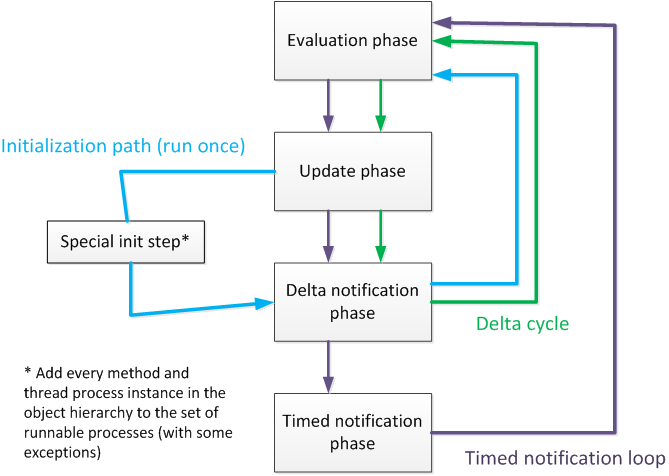
\includegraphics[width=\textwidth]{./tmp/systemc-scheduler.png}

\subsection{Специализированные языки}

Для решения специфических задач существуют предметно-ориентированные языки, предназначенные для разработки аппаратуры. Их использование рационально при условии, что они задействованы как часть большого пакета для моделирования систем.

\paragraph{Пример: DML}

Другим примером языка, специально созданного для описания функциональных моделей устройств, является DML (Device Modeling Language), используемый в симуляторе Simics~\cite{dml-tutorial}, в котором упор сделан на максимально быстрое модельное прототипирование устройств, т.е. создание заготовки устройства, не имеющей полной функциональности, но предоставляющей все внешние интерфейсы реального устройства. Этот подход позволяет реализовывать сложные системы постепенно, притом концентрироваться на самых  важных функциональных аспектах в первую очередь и дописывать недостающие компоненты после. Основной тип устройств, описываемых с помощью DML, — это неисполняющие устройства, он не используется для создания моделей процессоров.

Синтаксис DML предоставляет программисту конструкции для описания банков регистров, интерфейсов и функционального поведения устройств. Использование DML для написания модели автоматически гарантирует многие декларируемые Simics свойства у получаемых моделей.

\begin{itemize*}
\item Явное представление архитектурного состояния в \textit{атрибутах}.
\item Корректное сохранение и загрузка состояния симуляции из точек сохранения.
\item Безопасная многопоточность (\abbr thread safety).
\item Поддержка правильного порядка байт данных (т.н. Endianness) при взаимодействии моделей между собой.
\item Генерация текста документации из комментариев и строк описания деталей модели.
\end{itemize*}

Существующий компилятор \texttt{DMLC} является т.н. source-to-source компилятором, т.е. результатом его работы являются не машинные инструкции, а промежуточный текст на языке Си, который затем обрабатывается компилятором GCC. Однако при этом двухстадийном процессе сохраняется отладочная информация о строках исходного DML-кода, что позволяет использовать специально модифицированный вариант отладчика GDB, «понимающего» синтаксис DML для работы с исходным, а не с промежуточным кодом при отладке. Дополнительно этот подход позволяет при необходимости с помощью специальных команд языка включать код на Си в программу на DML, при этом такие куски передаются в промежуточный код без изменений.

\textbf{Пример кода на DML} % dammit I don't know why \paragraph does not work.

\begin{lstlisting}
register lcr { 
  parameter soft_reset_value = 0x00; 
  parameter hard_reset_value = 0x00; 
  field wls          [1:0] "Word length select "; 
  field stb          [2] "Number of stop bits (0 = 1, 1 = 2)"; 
  field pen          [3] "Parity enable (0 = disable, 1 = enable)"; 
  field eps          [4] "Even parity select (0=Odd, 1=Even)"; 
  field stick_parity [5] "Stick parity"; 
  field set_break    [6] "Set break"; 
  field dlab         [7] "Divisor latch access bit"; 
  // After a write to this register, check the contents of WLS and  
  // set the character length mask appropriately 
  method after_write (memop) { 
    if      ($wls == 0) $mask = 0x1F; 
    else if ($wls == 1) $mask = 0x3F; 
    else if ($wls == 2) $mask = 0x7F; 
    else                $mask = 0xFF; 
  } 
}   
\end{lstlisting} 


\subsection{Языки описания набора инструкций}

Отдельное внимание следует уделить разработке моделей процессоров и языкам, предназначенным для их создания.

Сложность данной задачи заключается в том, что при разработке совершенно нового устройства его авторам требуется иметь в рабочем состоянии одновременно  несколько инструментов и документов из следующего списка:

\begin{itemize*}
\item функциональный симулятор набора инструкций;
\item точная потактовая модель;
\item дизассемблер машинного кода;
\item компилятор с языка высокого уровня в машинный код;
\item документация к аппаратуре;
\item иногда необходимо также уметь генерировать синтезируемое описание новой архитектуры.
\end{itemize*}

Если каждая компонента разрабатывается отдельно, то при изменении спецификации процессора (что происходит часто на ранних этапах исследования) приходится вносить изменения во всех программах и документах, что чревато ошибками и десинхронизацией инструментов, каждый из которых фактически имеет собственный «взгляд» на одно и то же устройство.  

Существует несколько проектов языков, призванных решить всю описанную задачу. В качестве примера см. LISA~\cite{wahlen2004c,zivojnovic1996,schliebusch2002}, ISDL~\cite{Hadjiyiannis97isdl:an,isdl1997} и~\cite{hoffmann2001}. Решение состоит в автоматической генерации необходимых инструментов из одного описания (рис.~\ref{fig:lisa}). 

\begin{figure}[htb]
    \centering
	\inputpicture{drawings/lisa}
    \caption{Генерация инструментов разработки из общего описания архитектуры}
    \label{fig:lisa}
\end{figure}


Одним из недостатков этого подхода является зачастую субоптимальная скорость или качество работы получаемых инструментов; например, компилятор может генерировать не самый быстрый или компактный код, функциональная модель работает медленнее, чем могла бы будучи написанной человеком, синтезируемое описание занимает излишне много места на кристалле и т.д. Тем не менее скорость создания, модификации и степень согласованности всех инструментов часто перевешивают эти огрехи на ранних этапах, а затем, после фиксации спецификаций, все инструменты могут быть переписаны «вручную», с необходимыми оптимизациями.

Другой аспект, возникающий при создании моделей процессоров — желание иметь её с более чем одним механизмом симуляции, например, создать интерпретатор и двоичный транслятор и затем иметь возможность переключаться между ними. И снова для того, чтобы избежать рассинхронизации суб-моделей при правках спецификаций, чаще всего избирается подход,  при котором они генерируются из одного описания семантики инструкций~\cite{simgen, sled1997}.

Для построения двоичных трансляторов также может использоваться преобразование описаний семантики гостевых инструкций в заготовки машинного кода, при этом исходное описание является неким метаассемблером, преобразуемым в настоящий ассемблер хозяйской архитектуры (рис.~\ref{fig:capsules}). Такой подход позволяет разработчику иметь наибольший контроль над создаваемым двоичным транслятором~\cite{MyConfMIPT52}. Существенным недостатком является полная непереносимость модели на другую хозяйскую архитектуру, т.к. при этом приходится переписывать весь код эмуляции инструкций.

\begin{figure}[htb]
    \centering
	\inputpicture{drawings/capsules}
    \caption[Создание двоичного транслятора из метаассемблера]{Создание двоичного транслятора из метаассемблера. Исходное описание содержит в себе аргументы создаваемой функции и ассемблерные инструкции хозяйской архитектуры. После процесса обработки мы имеем два блока исходного кода — ассемблерный код, используемый при симуляции, а также код на Си (эмиттер), передающий первому аргументы на этапе трансляции}
    \label{fig:capsules}
\end{figure}


% \subsection{Bluespec}

% \todo Описать.

% Arvind had developed the Bluespec language, a high-level functional hardware description programming language which was essentially Haskell extended to handle chip design and electronic design automation in general. Bluespec is partially evaluated (to convert the Haskell parts) and compiled to the term rewriting system. The justification behind writing chip designs in Bluespec is that it leads to shorter, more abstract, and verifiable (provably correct) source code, as well as type-checked numeric code. Bluespec, Inc. claims greater than 50\% improvements compared to conventional methods of design[citation needed]. It also comes with a SystemVerilog frontend.

% Bluespec is the only ESL synthesis solution for control logic, complex datapaths and algorithms[citation needed]. For SystemC users, Bluespec has delivered high-level ESL Synthesis abstractions to SystemC. Bluespec integrates seamlessly into Cadence, Synopsys, Mentor and Magma flows, including verification, debug and synthesis, without requiring new methodologies or tools.


\section{Языки разработки аппаратуры}

В заключение кратко познакомимся с двумя самыми популярными языками описания аппаратуры (\abbr Hardware Definition Language, HDL), используемыми в настоящее время — Verilog и VHDL.

\subsection{Verilog}
 
Verilog был создан Филом Мурби и Прахбу Гоелом в  1984 году в фирме Auto\-mated In\-te\-gra\-ted De\-sign Sys\-tems. Он был принят как стандарт IEEE 1364-1995. Позже дополнения к языку Verilog-95 были приняты как IEEE 1364-2001 (или Veri\-log-2001). Следующий вариант, Verilog 2005 (стандарт IEEE 1364-2005), добавил небольшие исправления, уточнения спецификаций и несколько новых синтаксических конструкций.

Разработчики Verilog сделали его синтаксис очень похожим на синтаксис языка C, что упрощает освоение. Язык имеет препроцессор, очень похожий на препроцессор языка C, и основные управляющие конструкции \texttt{if}, \texttt{while} также подобны одноимённым конструкциям языка C. 

Существует подмножество инструкций языка Verilog, называемое синтезируемым. Модули, которые написаны на этом подмножестве, называют \textit{RTL} (\abbr register transfer level — уровень регистровых передач). Они могут быть физически реализованы с использованием САПР-синтеза. Данные САПР по определённым алгоритмам преобразуют абстрактный исходный код на Verilog в \emph{netlist} — логически эквивалентное описание, состоящее из элементарных логических примитивов (например, AND, OR, NOT, триггеры), которые доступны в выбранной технологии производства СБИС или программирования БМК и ПЛИС. Дальнейшая обработка netlist в конечном итоге порождает фотошаблоны для литографии или прошивку для FPGA.

Что отличает этот язык от обычных языков общего назначения? Во-первых, разделение всех команд на \textit{синтезируемые}, т.е. непосредственно представляемые в аппаратуре, и на \textit{несинтезируемые}, используемые только для отладки и симуляции.

Оператор \texttt{<=} в Verilog является ещё одной особенностью языка описания аппаратных средств, отличающей его от процедурных языков общего назначения. Сама операция известна как \textit{неблокирующее присваивание}. Применение оператора не имеет внешне видимого эффекта до наступления следующего такта. Это означает, что порядок таких присваиваний в коде не может влиять на суммарный эффект функции, т.к. все они произойдут одновременно и произведут тот же результат: значения \texttt{flop1} и \texttt{flop2} будут обмениваться значениями на каждом такте.

Другой оператор присваивания, <<\texttt{=}>>, является блокирующим. Когда он используется, переменная с его левой стороны обновляется немедленно. В приведённом выше примере, если бы использовался <<\texttt{=}>> вместо <<\texttt{<=}>>, \texttt{flop1} и \texttt{flop2} не обменялись бы значениями. Вместо того, как и в традиционном процедурном программировании, компилятор воспринял бы это как указание сделать их содержимое одинаковым.

\textbf{Пример кода на Verilog: триггер} % dammit I don't know why \paragraph does not work.

\begin{lstlisting}
module toplevel(clock,reset);
 input clock;
 input reset;
 reg flop1;
 reg flop2;
 always @ (posedge reset or posedge clock)
 if (reset)
   begin
     flop1 <= 0;
     flop2 <= 1;
   end
 else
   begin
     flop1 <= flop2;
     flop2 <= flop1;
   end
endmodule         
\end{lstlisting}

\paragraph{SystemVerilog} \cite{systemverilog-ru} — язык описания и верификации аппаратуры, являющийся расширением языка Verilog, вобравший в себя некоторые черты других языков описания аппаратуры: Superlog и OpenVera. Язык был стандартизирован как IEEE 1800—2005, а позднее он был объединён с Verilog в единый язык (стандарт IEEE 1800—2009). Были добавлены новые типы данных, представлена концепция интерфейсов, используемых для группировки портов. Главным расширением языка по сравнению с Verilog является введение средств для проведения верификации моделей, основанных на объектно-ориентированной парадигме. При этом новые конструкции не входят в синтезируемое подмножество языка.

\subsection{VHDL}

VHDL был разработан в 1983 г. по заказу Министерства обороны США с целью формального описания логических схем для всех этапов разработки электронных систем, начиная с модулей микросхем и заканчивая крупными вычислительными системами.

Первоначально язык предназначался для моделирования, но позднее из него было выделено синтезируемое подмножество. Средствами языка VHDL возможно проектирование на различных уровнях абстракции (поведенческом или алгоритмическом, регистровых передач, структурном) в соответствии с техническим заданием и предпочтениями разработчика. Представляется возможным выделить следующие три составные части языка: алгоритмическую, основанную на языках Ada и Pascal и придающую языку VHDL свойства процедурных языков, и проблемно ориентированную, обращающую VHDL в язык описания аппаратуры, а также объектно-ориентированную, интенсивно развиваемую в последнее время.

\textbf{Пример кода на VHDL} % dammit I don't know why \paragraph does not work.

\begin{lstlisting}
-- latch template 1:
Q <= D when Enable = '1' else Q;
-- latch template 2:
process(D,Enable)
begin
  if Enable = '1' then
    Q <= D;
  end if;
end process;
\end{lstlisting} 

\section{\Questions к главе \ref{lang}} %\label{lang-questions}

\subsection*{Вариант 1}

\begin{questions}

\question[3] Какое утверждение наилучшим образом характеризует термин SystemC?
\begin{choices}
    \choice Компилятор языка Си с дополнениями для моделирования систем.
    \choice Язык программирования, похожий на Си.
    \choice Язык программирования, похожий на С++.
    \correctchoice Набор библиотек для С++.
\end{choices}

\question[3] Язык DML используется для разработки
\begin{choices}
    \correctchoice функциональных моделей,
    \choice потактовых моделей,
    \choice гибридных моделей.
\end{choices}

\question[3] Текущая реавлизация комилятора DMLC является
\begin{choices}
    \choice компилятором типа source-to-source с промежуточным языком С++,
    \choice компилятором, преобразующим исходный текст в байткод Java,
    \correctchoice компилятором типа source-to-source с промежуточным языком Си,
    \choice классическим компилятором,
    \choice частичным интерпретатором.
\end{choices}

\question[3] Закончите фразу: Языки разработки аппаратуры
\begin{choices}
\choice не используются для начального моделирования устройств, так как могут быть преобразованы только в netlist,
\correctchoice не используются для начального моделирования устройств, так как получаемые модели очень медленны,
\choice не используются для начального моделирования устройств, так как могут содержать в себе синтезируюмую часть,
\choice используются для начального моделирования устройств.
\end{choices}

\question[3] Что означает уровень <<X>> на входе логического элемента цифровой схемы?
\begin{choices}
    \correctchoice Фактическое значения сигнала не влияет на работу узла.
	\choice Напряжение на входе ниже значения, используемого для кодирования логического нуля.
    \choice Контакт не подключен ни к одному выходу схемы.
	\choice Cопротивление между входом и выходом сигнала очень велико.
\end{choices}

\end{questions}

\subsection*{Вариант 2}

\begin{questions}

\question[3] Какое утверждение наилучшим образом характеризует термин <<TLM>>?
\begin{choices}
    \choice Язык программирования, похожий на Си.
    \choice Язык программирования, похожий на С++.
    \choice Среда исполнения моделей DES.
    \correctchoice Развитие стандарта SystemC.
\end{choices}

\question[3] Язык DML используется для разработки
\begin{choices}
    \correctchoice неисполняющих моделей,
    \choice исполняющих моделей,
    \choice как исполняющих, так и неисполняющих моделей.
\end{choices}

\question[3] Какой способ наиболее удобен и надёжен для поддержания набора инструментов моделирования в синхронизированном состоянии при постоянном изменении входной спецификации процессора?
\begin{choices}
    \correctchoice Генерация всех инструментов из единого описания.
    \choice Тщательное сравнение всех инструментов после каждого изменения одного из них.
    \choice Создание одного инструмента, поддерживающего максимальное количество функций.
\end{choices}

\question[3] Закончите фразу: Синтезируемое подмножество языков разработки аппаратуры
\begin{choices}
\choice не может быть использовано для создания netlist и RTL-описаний,
\choice используется только для отладки моделей,
\correctchoice  используется для создания netlist и RTL-описаний.
\end{choices}

\question[3] Что означает уровень <<Z>> на входе логического элемента цифровой схемы?
\begin{choices}
    \correctchoice Контакт не подключен ни к одному выходу схемы.
	\choice Сигнал непрерывно изменяется в течение всего такта.
    \choice Фактическое значения сигнала не влияет на работу узла.
	\choice Напряжение на входе превышает значение, используемое для кодирования логической единицы.
\end{choices}

\end{questions}

% К каждой лекции должно быть от 8 до 12 задач, у каждой задачи должно быть 3-5 вариантов формулировок примерно одинаковой сложности. Допускается объединение нескольких последовательных лекций в одну тему и подготовка тестов к темам.
% Задачи должны полностью соответствовать материалам лекций, то есть лекциях должно быть достаточно информации для ответа на все вопросы.
% Формулировка каждого варианта задачи должна содержать всю необходимую информацию и не должна ссылаться на тексты внутри лекции, картинки или другие задачи или варианты задачи.
% Правильные ответы выделяются знаком «+» перед их формулировкой. Правильных ответов может быть несколько. Для тестов с несколькими ответами как минимум один ответ должен быть правильным и как минимум один ответ должен быть неправильным. 
% 
% Структура теста к лекции
% 
% \subsection*{Задача 1}
% 
% \paragraph{Вариант 1} 
% 
%     Чему равно 2+2?
%         Ответ 1. 3
%         + Ответ 2. 4
%         …
%         Ответ N. 5
% \paragraph{Вариант 2}
%     Чему равно 2*2?
%         + Ответ 1. 4
%         + Ответ 2. 2+2
%         …
%         Ответ N. 5
% \paragraph{Вариант 3}
% 
%     Чему равно 2-2?
%         Ответ 1. 0
% 
% 
%         
% \section{Просто подборка вопросов}
% 

\iftoggle{webpaper}{
    \printbibliography[title={Литература}]
}{}




\chapter{Взаимодействие симуляции с~внешним миром}\label{paravirt}

\dictum[Дмитрий Гайдук. Про олдовых людей]{Мимо люди разные ходят, но никто внимания не обращает: эка невидаль, в~самом деле, два олдовых человека реальность проткнуть пытаются.}

\section[Необходимость взаимодействия]{Необходимость взаимодействия симуляции и реальности}

Как и большинство прикладных программ, симуляторы не создаются по мотивам философской концепции «вещи в себе», а имеют средства взаимодействия с человеком. Пользователю необходимо как вводить некоторые данные в систему, так и получать её отклик, ради которого она и создавалась. Выделим два класса для таких активностей.

\begin{enumerate*}
\item \textit{Взаимодействие с моделью, повторяющее действия, осуществляемые с её физическим прототипом.} Если у реального компьютера есть клавиатура и оператор может нажимать её клавиши, нечто аналогичное должно быть у симулируемой модели. Если в конфигурации присутствует монитор или иное средство для вывода информации, оно в той или иной форме должно быть и в модели. 

\begin{figure}[htp]
    \centering
    % \includegraphics[width=0.8\textwidth]{./isolate-crop.pdf}
\begin{tikzpicture}[>=latex, font=\small, node distance=0.3cm, inner sep=0pt]
    
    \node (tower) {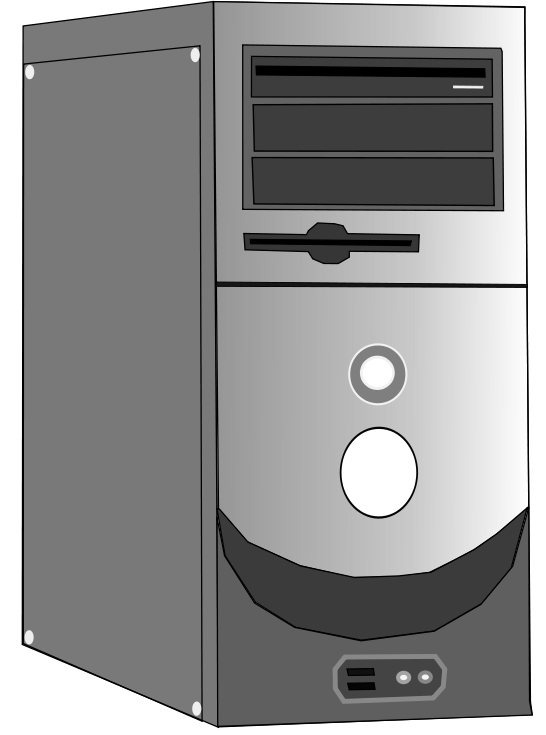
\includegraphics[height=1.5cm]{./tower.png}};
    \node[above=of tower] (monitor1) {
\includegraphics[height=1.2cm]{./monitor1.png}};
    \node[right =0.2cm of monitor1] (kb1) {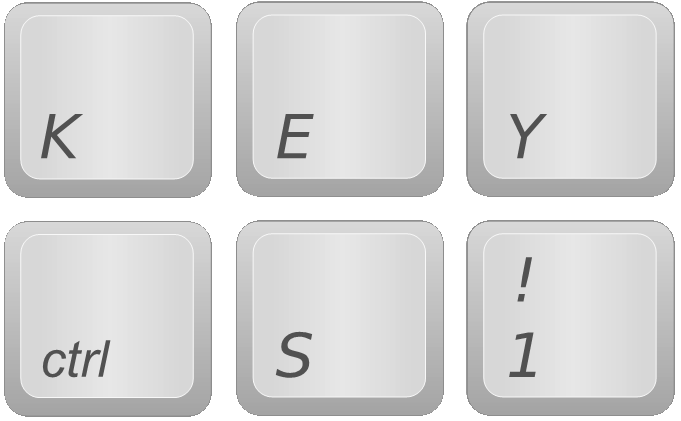
\includegraphics[height=.8cm]{./kb1.png}};
    
    % Inner border
    \node[draw, inner sep=0.2cm, fit=(tower) (monitor1) (kb1)] (virt) {};
    
    \node[right =2.cm of tower] (folder) {
\includegraphics[height=1.cm]{./folder.png}};
    \node[right =0.2cm of folder] (hdd) {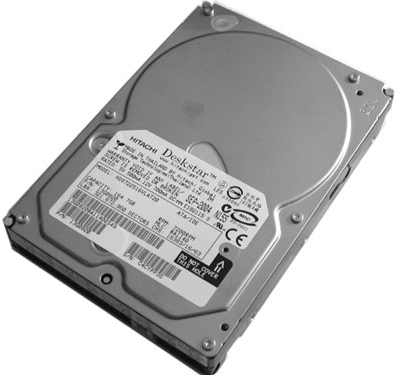
\includegraphics[height=1.cm]{./device3.png}};
    
    \node[right=0.7cm of hdd] (stub) {};
    
    % The outer border
    \node[draw, inner sep=0.35cm, fit= (virt) (tower) (monitor1) (kb1)  (hdd) (stub)]  (real) {};
    
    \node[right =0.2cm of hdd] (nic) {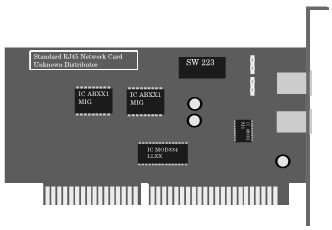
\includegraphics[height=1.cm]{./nic.png}};
    \node[right =of kb1, yshift=1cm] (kb2) {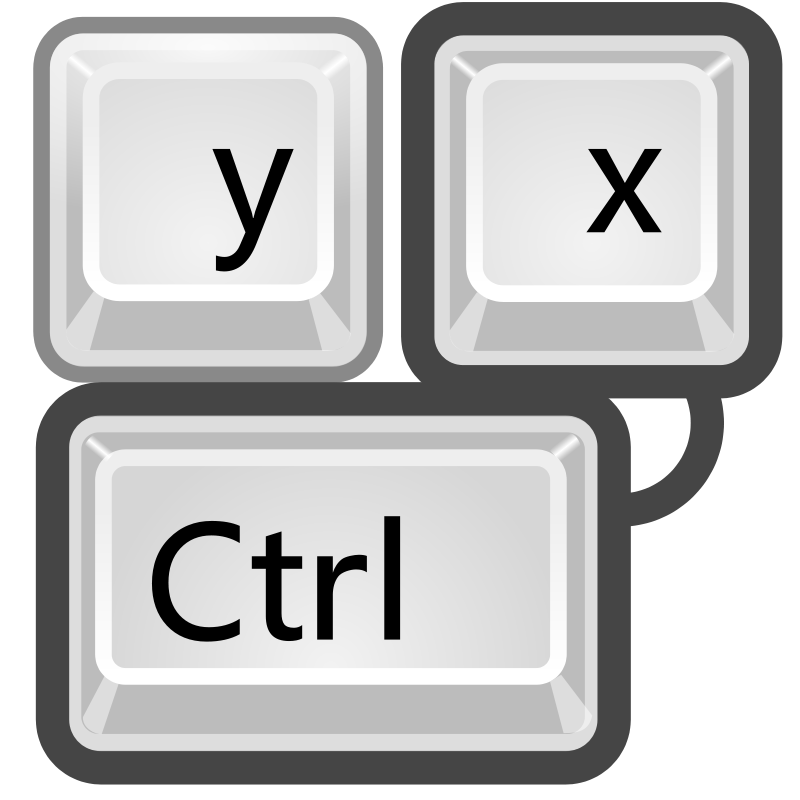
\includegraphics[height=1.5cm]{./kb2.png}};
    \node[right =of kb2] (monitor2) {
\includegraphics[height=1.5cm]{./monitor2.png}};   
    
    \node[fill=white, font=\scriptsize] at (virt.south) {Граница ВМ};
    
    \node[fill=white, font=\scriptsize] at (real.south) {Граница реальной системы};
\end{tikzpicture}
    \caption{Изоляция симулируемой системы от внешней среды}
    \label{fig:isolate}
\end{figure}

Симулируемое окружение вступает во взаимодействие с настоящим миром, находящимся вне модели, со всеми вытекающими из этого обстоятельствами, например невозможностью гарантировать повторяемость симуляций: даже если человек нажимает одни и те же клавиши в различных запусках модели, длительность и паузы между ними всегда будут различными.

Отметим, что полная аналогичность пользовательского интерфейса необязательна --- так, ввод с клавиатуры для модели на самом деле может идти из заранее записанного файла, расположенного на хозяйской файловой системе, а вывод видеокарты --- сохраняться в сетевой поток, транслируемый на удалённый сервер.

\item \textit{Инспектирование состояния модели и вмешательство в её работу, неосуществимые на реальной аппаратуре.} Сюда входит чтение содержимого регистров, памяти, их изменение «вручную», остановка симулируемого времени и т.п. Такие действия чаще всего не имеют соответствия в сценариях работы аппаратуры в реальном мире.
\end{enumerate*}

\section{Паравиртуализационные расширения}

Согласно принципу полной изоляции виртуализированного окружения находящаяся в нём программа не должна иметь возможностей отличить ситуацию, когда она выполняется на реальной аппаратуре, от работы внутри виртуального окружения. Это условие очень важно, так как позволяет использовать одно и то же программное обеспечение без необходимости модификаций и применять результаты, полученные на модели (доказательства корректности, предсказания производительности, энергопотребления и т.п.), к реальности.

Однако часто оказывается выгодным «пробить» изоляцию для увеличения производительности симуляции, повышения удобства пользования или получения новых сценариев взаимодействия окружений. При этом гостевое приложение или ОС модифицируются таким образом, чтобы задействовать некоторую функциональность аппаратуры, присутствующую только внутри модели, но не на реальных системах. Этот приём имеет общее название \textit{паравиртуализация}.

\subsection{Волшебные инструкции}

Для того чтобы иметь возможность совершать некоторые действия по достижении приложением некоторого этапа своей работы, можно использовать \textit{точки остановки симуляции} (\abbr breakpoints) по значению регистра-счётчика текущей инструкции. Иногда удобнее реагировать на исполнение некоторой специально выбранной инструкции вне зависимости от её адреса. В таком случае инструкция получает название «волшебной», т.к. с ней связаны необычные эффекты. С помощью такой инструкции мы можем помечать в приложении интересующие места, при этом на неё налагаются следующие ограничения.

\begin{itemize*}
\item    Инструкция не должна использоваться самим приложением, иначе мы будем получать ложные срабатывания и будем вынуждены как-то фильтровать их.
\item    Желательно, чтобы она несла минимальную семантическую нагрузку, что позволило бы использовать её во многих сценариях. Так, желательно, чтобы инструкция не была неопределённой на реальной аппаратуре, иначе приложение с ней не будет корректным вне симулятора. 
\item В идеале она должна сохранять неизменным содержимое памяти, работать во всех режимах процессора, предсказуемо менять счётчик инструкций, т.е. не быть инструкцией перехода. 
\end{itemize*}

Второму условию наилучшим образом отвечают варианты инструкции NOP --- no operation. В самом деле, подобная инструкция изменяет архитектурное состояние минимальным образом (т.к. на её исполнение всё-таки тратится время). Однако компиляторы часто используют NOP для своих целей выравнивания кода и т.п., что не соответствует первому условию. Исключением является архитектура IA-32, где имеются две инструкции NOP --- классическая однобайтовая (\texttt{0x90}) и  расширенная (\texttt{0x0F 0x1F /0})~\cite{intelmanual2a}; последняя может иметь длину от трёх до девяти байт и один операнд. Она является хорошим кандидатом для того, чтобы стать «волшебной» внутри симуляции.

Другой альтернативой являются недокументированные инструкции, которые не встречаются в приложениях. Однако их неопределённая функциональность на реальной аппаратуре ограничивает удобство использования.

Третьим вариантом можно считать инструкции с необычными аргументами, префиксами и другими особенностями, не встречающиеся в обычном коде. Например, для архитектуры IA-32 это может быть \texttt{CPUID} с операндами вне допустимого диапазона, инструкции с префиксами, не влияющими на её исполнение и т.п.

\begin{figure}[htp]
    \centering
    % \includegraphics[width=0.6\textwidth]{./magic-inst-crop.pdf}
\begin{tikzpicture}[>=latex, font=\small]
    \node (tower) {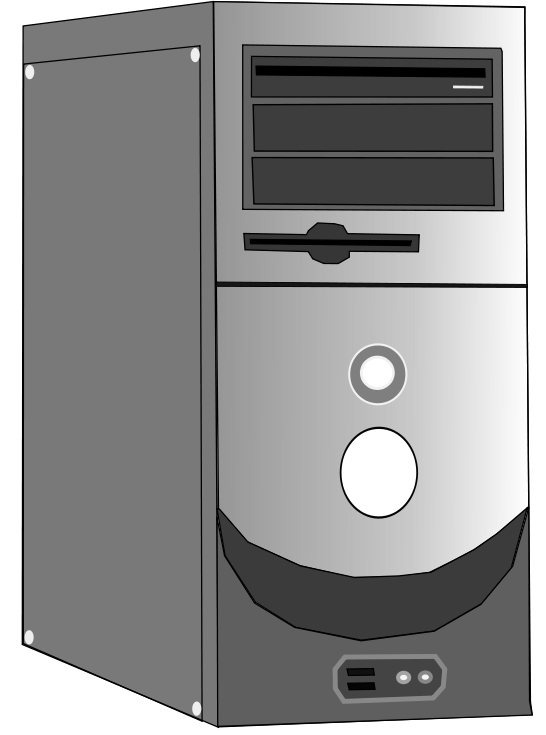
\includegraphics[height=1.5cm]{./tower.png}};
    \node[right =0.25cm of tower] (folder1) {
\includegraphics[height=1.cm]{./folder.png}};
    \node[right=0.5cm of folder1] (stub) {};
    \node[draw, fit=(tower) (folder1) (stub), inner sep=2pt] (virt) {};
    
    \node[right =0.1cm of folder1, double arrow, draw, fill=white] (arrow) {1 байт};
    \node[right =0.1cm of arrow] (folder2) {
\includegraphics[height=1.cm]{./folder.png}};
    \node[draw, fit=(tower) (folder1) (folder2), inner sep=0.5cm] (real) {};
    
    \node[fill=white, font=\scriptsize, inner sep=1pt] at (virt.south) {Граница ВМ};
    \node[fill=white, font=\scriptsize, inner sep=1pt] at (real.south) {Граница реальной системы};
\end{tikzpicture}    
    \caption{Передача файлов с помощью магических инструкций}
    \label{fig:magic-inst}
\end{figure}

\subsection{Паравиртуальные устройства}

Сценарий использования «волшебной» инструкции, описанный ранее, передаёт лишь один бит информации между гостем и хозяином --- это сам факт присутствия. Часто возникает необходимость передать большие объёмы информации. Несколько байт ещё могут вместиться как операнды инструкции или в регистрах процессора. Для передачи большего объёма данных за один раз необходимо иметь больший буфер для данных. Самым очевидным представляется выделить для этого часть физического адресного пространства гостя. Чтобы чтения и записи этого диапазона обрабатывались симулятором, с ним ассоциируется псевдоустройство; запись в ассоциированную с ним память вызывает приостановку симуляции и обработку новых данных. О способе использования этого механизма рассказывается в следующей секции.

\subsection[Ускорение ввода-вывода]{Ускорение ввода-вывода через периферийные устройства}

Виртуализация выступает как дополнительная «обёртка» между виртуальными и реальными устройствами ввода-вывода (установленными в PCI, PCI-Express слоты расширений, подключенными к IDE и SATA шинам дисками и т.п.), что приводит к необходимости двойной (иногда тройной) передаче данных --- один раз внутри модели, второй --- в реальной системе. Это приводит к копированию больших объёмов данных из одной области памяти в другую без какой-либо обработки и сильно ограничивает скорость работы высокоскоростных периферийных устройств.

Для ускорения необходимо избавиться от прослойки симуляции для определённых устройств. Реализуется это модификацией гостевой операционной системы --- в неё включаются драйвера паравиртуальных устройств, способных напрямую инструктировать виртуальную машину о необходимости передачи данных.

Изменённое ядро является недостатком этого подхода и существенно ограничивает его применимость для систем, коды/интерфейсы ядра которых закрыты.

\subsection{Проброс устройства}

Иногда представляется возможным перенаправлять все запросы на доступ к некоторому устройству прямо из гостя, без обработки команд симулятором. Это требует вмешательства уже в хозяйскую ОС, так как обычно она ограничивает  прямой доступ к аппаратуре со стороны пользовательских приложений.

В случае паравиртуализации периферийное устройство может быть разделено между хозяином и несколькими гостями. При \textit{пробросе} (\abbr pass through) оно полностью отдаётся в распоряжение одному из них. Пример эксклюзивного использования хозяйских устройств --- проброс USB-устройств в Oracle Virtualbox; при этом оно пропадает в хозяйской системе до тех пор, пока подключено внутри виртуальной машины.

В современных материнских платах появилась аппаратная поддержка виртуализации периферийных устройств, что избавляет виртуальные машины от ещё одного уровня косвенности --- он переносится в «железо». Что интересно, уровень позволяет также эффективно использовать одно устройство в нескольких независимых изолированных окружениях. Например, сетевая карта при этом будет иметь несколько независимых MAC-адресов, что зачастую избавляет от необходимости использования паравиртуализации. Примеры таких технологий --- Intel VT-d и AMD IOMMU.

\subsection{Дополнительные каналы передачи данных}

Описанные выше техники в общем случае позволяют внести в симулируемое окружение дополнительные способы обмена данными между хозяином и гостем. При этом паравиртуализация может проявляться на разных уровнях программного стека гостевой ОС, а не только на уровне драйверов устройств. Например, <<волшебные инструкции>> могут быть использованы для реализации утилиты копирования  отдельных файлов (в общем случае --- потока байт) между гостем и хозяином. Если требуется более тесная интеграция, то может быть использован драйвер файловой системы для монтирования директории машины хозяина внутри гостя, при этом все изменения, сделанные внутри гостя, становятся видны снаружи в хозяине. Такая функциональность существует во многих популярных виртуальных машинах, например в виде файловых систем \texttt{hostfs} в составе Simics или \texttt{vboxsf} из состава гостевых дополнений Virtualbox.

\section[Интерактивные устройства]{Интерактивные устройства для~взаимодействия с пользователем}

Простейшее средство для общения пользователя с системой может быть представлено двумя односторонними потоками символов. Базовое устройство, предоставляющее такой функционал, --- это последовательный порт RS-232. Несмотря на приличный возраст стандарта и невысокую скорость передачи данных (до 115,2 кбит/c), он до сих пор является популярным интерфейсом для многих приложений, поддерживается практически всеми существующими операционными системами и доступен на самых ранних этапах загрузки ЭВМ. Часто именно этот вид периферийного устройства реализуется в новом симуляторе в первую очередь. 

Ввиду простоты используемой абстракции передачи данных модель последовательного порта со стороны реального мира может быть использована множеством способов. Например, возможно подключение к эмулятору терминала и использование модели для интерактивного взаимодействия с пользователем. Выходящий поток  будет записываться в файл, а ввод-вывод --- перенаправлен в сетевой сокет, именованный канал Unix/Windows, символьное  устройство или виртуальный параллельный порт или даже подключен к реальному порту хозяйской системы.

Более сложными с точки зрения моделирования устройствами ввода являются клавиатура и мышь. Существуют варианты их подключения к материнской плате через различные интерфейсы: последовательный порт, PS/2, USB\dots\ Клавиатура должна моделировать события нажатия и отпускания, а также допускать возможность одновременного нажатия нескольких клавиш. Способы подключения к реальности, как и в случае последовательного интерфейса, могут быть разнообразными.

Наиболее популярным устройством вывода графической информации является монитор. Его моделирование подразумевает создание сложного комплекса моделей: от PCI (Express) или AGP слотов на материнской плате до видеокарты, далее через цифровую начинку монитора к его дисплею. Серьёзная задача состоит в обеспечении достаточной скорости прорисовки изображения, формируемого гостем, особенно если это трёхмерные сцены или интенсивная двухмерная графика (видео). В таких сценариях использования «программная» эмуляция только средствами центрального процессора хозяина, как правило, неспособна обеспечить комфортную для пользователя частоту обновления экрана. Решение состоит в задействовании аппаратных ресурсов хозяйской машины, осуществляемое либо через паравиртуализацию, либо пробросом PCI устройства в гостевую систему.

\section{Диски}

Под дисками мы будем подразумевать устройства хранения данных на жёстких магнитных дисках (стандарты SATA, IDE, FireWire, SCSI), твердотельных накопителях (USB-флешки, SSD), а также оптические диски (CD, DVD, Blu-ray) и теряющие актуальность гибкие диски (\abbr floppy disks).

С моделированием дисковой подсистемы связано несколько специфичных вопросов.

\begin{itemize*}
\item Обеспечение высокой скорости симуляции. Объём передаваемых данных для ряда приложений может быть большим, как и связанное с этим замедление модели.

\item Обеспечение непосредственного хранения массивов данных. Ёмкость моделируемых дисков может достигать десятков терабайт.
\item Постоянство хранилища модели. В отличие от ОЗУ и регистров устройств, жёсткие диски не теряют данные при выключении или перезагрузке компьютера. Однако сохранение состояния между запусками симуляции нарушает принцип её воспроизводимости и повторяемости.
\end{itemize*}

\subsection{Скорость}

В общем случае замедление связано с необходимостью многократного копирования данных между симуляцией и реальной системой хранения. Как было описано раньше, сценарии решения этой проблемы заключаются в паравиртуализации или в пробросе устройства внутрь симуляции.

\subsection{Форматы хранения}

Поскольку диск представляет собой устройство с произвольным доступом, естественная форма хранения его данных --- это файл в хозяйской системе, блоки содержимого которого соответствуют данным гостевого диска.

В простейшем случае файл должен содержать просто копию байт-в-байт всего содержимого реального диска, это т.н. «сырой» (\abbr raw) образ диска (рис.~\ref{fig:raw}). При этом все сектора гостевого диска расположены последовательно в том же порядке, который они имели бы  в реальности. Преимущество такого способа хранения --- его простота и универсальность. Процесс создания сырого образа физического носителя обычно очень прост\footnote{Например, это можно сделать с помощью Unix-утилиты \texttt{dd}.}. Очень многие существующие симуляторы поддерживают образы в <<сыром>> формате. Основной его недостаток --- нерациональность использования ресурсов хозяина. Например, симуляция установки ОС может занять 1 Гбайт места на образе диска в 100 Гбайт; результирующий образ диска будет занимать 100 Гбайт, при этом 99\% его будут потеряны для хозяйской системы впустую.

\begin{figure}[htb]
    \centering
    % \includegraphics[width=0.8\textwidth]{./raw-format-crop.pdf}
\begin{tikzpicture}[>=latex, font=\small]
    \path (0,0.5) coordinate (a1);
    \draw (0,0) rectangle (7.5,1);
    \node[left = 0.25cm of a1] (host-disk) {Хозяйский диск};
    
    \draw (3,-2) rectangle (6,-1);
    \node[below = 1.5cm of host-disk] {Гостевой диск};
    
    \draw[fill=black!5] (3,0) rectangle (6,1);
    \draw[dotted] (3,-1) -- (3,0);
    \draw[dotted] (6,-1) -- (6,0);
    
    \path[fill=black!20] (4,0) rectangle (4.5,1);
    \path[fill=black!20] (5,0) rectangle (5.5,1);
    
    \path[fill=black!20] (4,-2) rectangle (4.5,-1);
    \path[fill=black!20] (5,-2) rectangle (5.5,-1);
    
    \draw[<->] (4.25,-1) -- (4.25,0);
    \draw[<->] (5.25,-1) -- (5.25,0);
    
    \path (4.5,-2) coordinate (a2);
    \node[below =0.25cm of a2, inner sep=1pt] (used) {Используемые области};
    
    \draw[dotted] (used) -- (4.25,-2);
    \draw[dotted] (used) -- (5.25,-2);
    
    \draw[decorate, decoration={brace, amplitude=3pt}, yshift=3pt] (3,1) -- (6,1) coordinate[midway] (a3);
    \node[above = 0.1cm of a3] {Образ диска};    
\end{tikzpicture}
    \caption[<<Сырой>> образ диска]{<<Сырой>> образ диска. Хранится каждый сектор, даже если он не задействоован внутри гостевой системы, что приводит к нерациональному расходованию места}
    \label{fig:raw}
\end{figure}

Многие симуляторы поддерживают более компактные способы хранения, в которых в файл записываются только изменённые секторы диска; заголовочная часть файла содержит список этих секторов и их местоположение (рис.~\ref{fig:compat}). Как правило, каждая программа имеет свой формат и иногда поддерживает другие или позволяет конвертировать их друг в друга. Примеры: Qcow2~\cite{qcow2} (Qemu), VDI (Oracle Virtualbox), VMDK~\cite{vmdk} (VMware ESX), VHD (Microsoft VirtualPC), HDD (Parallels Desktop), CRAFF (Wind River Simics).

\begin{figure}[htb]
    \centering
    % \includegraphics[width=0.8\textwidth]{./compat-crop.pdf}
\begin{tikzpicture}[>=latex, font=\small]
    \path (0,0.5) coordinate (a1);
    \draw (0,0) rectangle (7.5,1);
    \node[left = 0.25cm of a1] (host-disk) {Хозяйский диск};
    
    \draw (3,-2) rectangle (7,-1);
    \node[below = 1.5cm of host-disk] {Гостевой диск};
    
    % \draw[fill=black!5] (3,0) rectangle (6,1);
    % \draw[dotted] (3,-1) -- (3,0);
    % \draw[dotted] (6,-1) -- (6,0);
    
    \path[thick, fill=black!25] (1.2,0) rectangle (1.49,1);
    \path[fill=black!20] (1.51,0) rectangle (2.49,1);
    \path[fill=black!20] (2.51,0) rectangle (3.5,1);
    
    \path[fill=black!20] (4.,-2) rectangle (4.99,-1);
    \path[fill=black!20] (5.01,-2) rectangle (6,-1);
    
    \draw[<->] (4.25,-1) -- (2,0);
    \draw[<->] (5.25,-1) -- (3,0);
    
    \path (4.5,-2) coordinate (a2);
    \node[below =0.25cm of a2, inner sep=1pt] (used) {Используемые области};
    
    \draw[dotted] (used) -- (4.25,-2);
    \draw[dotted] (used) -- (5.25,-2);
    
    \draw[decorate, decoration={brace, amplitude=3pt}, yshift=3pt] (1.2,1) -- (3.5,1) coordinate[midway] (a3);
    \path (1.35,1) coordinate (a4);
    \node[above = 0.1cm of a3] {Образ диска};    
    \node[above = 0.5cm of a4, xshift=-2cm, inner sep=1pt] (header) {Заголовок};    
    \draw[dotted] (a4) -- (header);
    
\end{tikzpicture}
    \caption[Компактный формат образа диска]{Компактный формат образа диска. Хранятся только данные используемых секторов гостевого диска, а также служебная информация, описывающая их местоположение}
    \label{fig:compat}
\end{figure}

Некоторые форматы поддерживают прозрачное сжатие записанных данных, когда вместо обычной копии каждого гостевого сектора хранится его представление, полученное применением одного из известных алгоритмов сжатия без потерь, например Gzip, Bzip2 или LZMA~\cite{sayood2002lossless}.

Для образов оптических дисков, которые в большинстве  случаев являются носителями с данными только для чтения, используются сырые образы. Чаще всего они именуются ISO-образами по имени стандарта используемой на них файловой системы ISO 9660\footnote{Хотя это не единственный стандарт для оптических дисков; альтернативой является UDF (universal disk format), призванный обойти многие ограничения ISO 9660.}.

Из-за своего небольшого размера (меньше 3 Мбайт) образы гибких дисков хранятся в raw-формате.

\subsection{Сохранение состояния дисков}

Зачастую нежелательно модифицировать исходный файл образа диска: экспериментальное ПО/вирусы/ошибки пользователя внутри симулятора могут сделать его неработоспособным, или же желательно впоследствии запускать симуляцию из первоначального состояния.

Для таких целей в большинстве симуляторов существует опция: все изменённые секторы сохранять не в оригинальном, а в дополнительном \textit{разностном} файле (также называемом \textit{дельтой}). Для моделируемого приложения указанная схема абсолютно прозрачна --- внутри симуляции изменения видны там, где и должны быть. Однако после выключения симуляции допустимо отбросить дельту и использовать оригинальный образ. В случае появления желания зафиксировать внесённые в результате последней симуляционной сессии правки --- следует воспользоваться утилитами слияния оригинального образа и дельты.

Развивая эту идею, можно вообразить себе схему с несколькими дельтами, полученными на разных этапах симуляции (и даже <<дельты к дельтам>>), одновременно наложенными на диск. Таким образом, можно иметь множество снимков состояний дискового хранилища, суммарно занимающие места меньше, чем занимали бы отдельные полные копии.

\section{Сеть}

Современный Интернет был спроектирован так, чтобы обеспечивать обмен информацией между системами совершенно различной структуры, масштабов, используемых технологий. Взаимодействие симуляции и реальности через сеть является наиболее «естественным» подходом, поскольку у агентов имеются лишь самые общие предположения о свойствах друг друга.

Существует семь уровней абстракции данных OSI ISO~\cite{osi-iso-rus}. Ниже описана возможная классификация способов взаимодействия хозяина и гостя по их соответствию некоторым из этих уровней. Отметим, что такая классификация не является строгой и приводится для подчёркивания различий между ними.

\begin{itemize*}
\item    \textit{Физический уровень}. Для прозрачного использования гостевыми системами хозяйской сети необходимо иметь работающую модель сетевой карты (\abbr network interface card, NIC). Она может быть соединена с другими чисто программными моделями сетевых устройств (NIC, маршрутизаторами и т.д.) внутри симуляции или представлять собой проброшенную в симуляцию физическую NIC хозяйской системы.

\item    \textit{Канальный уровень}. Драйвер, именуемый TAP~\cite{tuntap}, обеспечивает модель сетевой карты и работает с кадрами Ethernet. Он устанавливается в хозяине. После этого хозяйская система может через новый интерфейс псевдо NIC взаимодейстовать с гостевой системой (при условии правильной настройки адресов и маршрутизации). Для того чтобы гость был представлен в том сегменте реальной сети, в котором находится хозяин, необходимо объединить в мост (\abbr bridge) одну из реальных и виртуальную карты. Очевидный недостаток --- хозяин теряет одно устройство NIC на каждой симуляции.

\item     \textit{Сетевой уровень}. TUN-драйвер обеспечивает более высокоуровневую модель и оперирует IP-пакетами, а не кадрами Ethernet. Такое соединение может использоваться для создания сетевого туннеля, например VPN. С точки зрения целей симуляции TUN не предоставляет существенных преимуществ над TAP.

\item    \textit{Транспортный уровень}. Для одностороннего доступа гостей к внешней сети, как правило, используется решение, в котором он размещается в отдельной подсети, а хозяин выступает как NAT-сервер. Все исходящие TCP-соединения выглядят как исходящие от хозяина. Недостаток данного подхода состоит в невозможности открыть соединение извне с симуляцией. Для обхождения этой проблемы используют переадресацию фиксированных номеров портов системы хозяина. Соединения на такие порты автоматически перенаправляются внутрь симуляции.

\item    \textit{Уровень приложений}. Для обеспечения работы некоторых гостевых приложений достаточно имитировать наличие в сети сервера, способного отвечать на их запросы. Например, виртуальный DHCP-сервер может раздавать IP-адреса симулируемым картам, виртуальный роутер обеспечивать NAT, виртуальный NFS- или Samba-серверы --- предоставлять доступ к части файловой системы хозяина.
\end{itemize*}

\section{\Questions к главе \ref{paravirt}} %\label{paravirt-questions}

\subsection*{Вариант 1}

\begin{questions}

\question[3] Выберите свойства, которые должны выполняться для идеальной <<волшебной>> инструкции:
\begin{choices}
    \correctchoice должна быть допустимой во всех режимах работы процессора,
    \choice должна быть привилегированной,
    \choice не должна иметь явных аргументов,
    \correctchoice не должна генерироваться обычными компиляторами,
    \correctchoice не должна вызывать эффектов (т.е. быть NOP),
    \choice не должна иметь неявных аргументов.
\end{choices}

\question[3] Какая инструкция для архитектуры IA-32 не может быть использована как волшебная?
\begin{choices}
\choice \texttt{CPUID} --- идентификация процессора,
\correctchoice \texttt{INT} --- программное прерывание,
\choice \texttt{NOP} --- пустая операция.
\end{choices}

\question[3] Для какой из перечисленных ниже операционных систем паравиртуализационные расширения сложно писать из-за закрытости исходного кода?
\begin{choices}
\correctchoice Microsoft Windows,
\choice GNU/Linux,
\choice FreeBSD.
\end{choices}

\question[3] В чём состоят недостатки сырого формата дисков?
\begin{choices}
\choice невозможность случайного доступа к секторам диска,
\choice нерациональное расходование дискового пространства гостя,
\correctchoice нерациональное расходование дискового пространства хозяина,
\choice отсутствие публичной документации на формат.
\end{choices}

\end{questions}

\subsection*{Вариант 2}

\begin{questions}

\question[3] Почему передача большого объёма данных между гостем и хозяином с помощью волшебной инструкции неэффективна?
\begin{choices}
\correctchoice за один раз можно передать только несколько байт,
\choice побочные эффекты множества волшебных инструкций подряд могут нарушить работу гостя,
\choice побочные эффекты множества волшебных инструкций подряд могут нарушить работу хозяина,
\choice направление передачи данных ограничено только направлением «гость → хозяин».
\end{choices}

\question[3] Назовите приём виртуализации, в котором гостевое приложение модифицируются таким образом, чтобы задействовать некоторую функциональность аппаратуры, присутствующую только внутри модели, но не на реальных системах?
\begin{choices}
\choice гиперсимуляция,
\choice метавиртуализация,
\correctchoice  паравиртуализация,
\choice изоляция.
\end{choices}

\question[3] Дайте определение термину <<проброс устройства>>:
\begin{choices}
\choice передача устройства в эксклюзивное пользование нескольким гостям,
\choice передача устройства в эксклюзивное пользование хозяину,
\correctchoice передача устройства в эксклюзивное пользование единственному гостю.
\end{choices}

\question[3] Для чего используются разностные файлы?
\begin{choices}
\correctchoice хранение изменений гостевого диска за время работы симуляции,
\choice сжатие оригинального образа гостевого диска для того, чтобы он занимал меньше места,
\choice прозрачное шифрование оригинального образа гостевого диска,
\choice расширения размера гостевого диска в случае, когда старый полностью заполнен.
\end{choices}

\end{questions}

% К каждой лекции должно быть от 8 до 12 задач, у каждой задачи должно быть 3-5 вариантов формулировок примерно одинаковой сложности. Допускается объединение нескольких последовательных лекций в одну тему и подготовка тестов к темам.
% Задачи должны полностью соответствовать материалам лекций, то есть лекциях должно быть достаточно информации для ответа на все вопросы.
% Формулировка каждого варианта задачи должна содержать всю необходимую информацию и не должна ссылаться на тексты внутри лекции, картинки или другие задачи или варианты задачи.
% Правильные ответы выделяются знаком «+» перед их формулировкой. Правильных ответов может быть несколько. Для тестов с несколькими ответами как минимум один ответ должен быть правильным и как минимум один ответ должен быть неправильным. 
% 
% Структура теста к лекции
% 
% \subsection*{Задача 1}
% 
% \paragraph{Вариант 1} 
% 
%     Чему равно 2+2?
%         Ответ 1. 3
%         + Ответ 2. 4
%         …
%         Ответ N. 5
% \paragraph{Вариант 2}
%     Чему равно 2*2?
%         + Ответ 1. 4
%         + Ответ 2. 2+2
%         …
%         Ответ N. 5
% \paragraph{Вариант 3}
% 
%     Чему равно 2-2?
%         Ответ 1. 0
% 
% 
%         
% \section{Просто подборка вопросов}
%

\iftoggle{webpaper}{
    \printbibliography[title={Литература}]
}{}


% Copyright (c) 2016 Grigory Rechistov <grigory.rechistov@phystech.edu>
% This work is licensed under the Creative Commons Attribution-NonCommercial-ShareAlike 4.0 Worldwide.
% To view a copy of this license, visit http://creativecommons.org/licenses/by-nc-sa/4.0/.

\chapter{Современная виртуализация}\label{virt}

\dictum[Harlan McGhan]{When this sort of deliberate disconnection from reality happens with people, it generally goes by names like deceit, fraud, misrepresentation, or simply lying. When it happens with computers, it’s called virtualization\footnotemark.}
\footnotetext{Когда подобный вид умышленного искажения реальности происходит в среде людей, его обычно называют обманом, мошенничеством, введением в заблуждение или просто ложью. Если же это происходит внутри компьютера, это зовётся виртуализацией.}

% Every day I look the same
% And the sun is always shining
% I look out and there is 3D
% I keep looking down and miss my shadow
% 
% Every day my hair is fine
% But one dot keeps changing colors
% I know my heritage is noble
% But still I feel like I'm a clone
% 
% 8 bits are enough for me
% This is not where I should be
% My life is more than information
% I want a life beyond emulation
% 
% I look out and every thing's too fast for me
% And I feel there must be more
% Every day I dream of where I've come from
% Now I know I'm just an emulation
% 
% The next time I see the serial cable
% I jump on the train and leave this world
% Now I'm an original, I'm like my ancestors
% And my hair is finally all yellow
% 
% 8 bits are enough for me
% This is not where I should be
% My life is more than information
%———--
% mind.in.a.box - 8 bits

\section{Введение}

Для понимания того, каким образом современные вычислительные системы, их новые свойства, инструкции и режимы призваны поддерживать виртуализацию, в этой главе мы рассмотрим теоретические основания возможности её \emph{эффективной} реализации. 

Виртуализация представляла интерес ещё до изобретения микропроцессора, во времена преобладания больших систем — мейэнфреймов, ресурсы которых были очень дорогими, и их простой был экономически недопустим. Виртуализация позволяла повысить степень утилизации таких систем, при этом избавив пользователей и прикладных программистов от необходимости переписывать своё ПО, так как с их точки зрения виртуальная машина была идентична физической. Пионером в этой области являлась фирма IBM с мэйнфреймами System/360, System/370, созданными в 1960--1970-х гг.

\section{Классический критерий виртуализуемости}

Неудивительно, что критерии возможности создания эффективного монитора виртуальных машин были получены примерно в то же время. Они сформулированы в классической работе 1974~г. Жеральда Попека  и Роберта Голдберга «Formal requirements for virtualizable third generation architectures»~\cite{popek}. Рассмотрим её основные предпосылки и сформулируем её основной вывод.

\subsection{Модель системы}

В дальнейшем используется упрощённое представление «стандартной» вычислительной системы, состоящей из (одного) центрального процессора и линейной однородной оперативной памяти. Периферийные устройства, а также средства взаимодействия с ними опускаются. Процессор поддерживает два режима работы: режим супервизора, используемый операционной системой, и режим пользователя, в котором исполняются прикладные приложения. Память поддерживает режим сегментации, используемый для организации виртуальной памяти.

Выдвигаемые требования на монитор виртуальных машин (ВМ): 

\begin{description*}

\item[Изоляция] — каждая виртуальная машина должна иметь доступ только к тем ресурсам, которые были ей назначены. Она не должна иметь возможности повлиять на работы как монитора, так и других ВМ.

\item[Эквивалентность] — любая программа, исполняемая под управлением ВМ, должна демонстрировать поведение, полностью идентичное её исполнению на реальной системе, \emph{за исключением} эффектов, вызванных двумя обстоятельствами: различием в количестве доступных ресурсов (например, ВМ может иметь меньший объём памяти) и длительностями операций (из-за возможности разделения времени исполнения с другими ВМ).

Отметим, что для симуляторов в общем смысле эквивалентность не является требованием, т.к. в случаях, когда хозяйская и гостевая архитектуры не совпадают, поведение гостя и хозяина различаются.

\item[Эффективность] — в оригинальной работе условие сформулировано следующим образом: «статистически преобладающее подмножество инструкций виртуального процессора должно исполняться напрямую хозяйским процессором, без вмешательства монитора ВМ». Другими словами, значительная часть инструкций должна симулироваться в режиме прямого исполнения. Требование эффективности является самым неоднозначным из трёх перечисленных требований, и мы вернёмся к нему в секции~\ref{sec:revising-efficiency}.

В случае симуляторов, основанных на интерпретации инструкций, условие эффективности не выполняется, т.к. каждая инструкция гостя требует обработки симулятором.

\end{description*}

\subsection{Классы инструкций}

Состояние процессора содержит минимум три регистра: $M$, определяющий, находится ли он в режиме супервизора $s$ или пользователя $u$, $P$ — указатель текущей инструкции и $R$ — состояние, определяющее границы текущего сегмента памяти\footnote{В простейшем случае $R=(l,b)$, где $l$ — адрес начала диапазона, $b$ — его длина.}. При исполнении каждая инструкция $i$ в общем случае может изменить как $(M,P,R)$, так и память $E$, т.е. она является функцией преобразования 

$$(M_1,P_1,R_1,E_1) \overset{i}\mapsto (M_2,P_2,R_2,E_2).$$ 

Память $E$ состоит из фиксированного числа ячеек, к которым можно обращаться по их номеру $t$, например, $E[t]$. Размер памяти и ячеек для данного рассмотрения несущественен.

Считается, что для некоторых входных условий инструкция вызывает исключение \textit{ловушки} (\abbr trap), если в результате её исполнения содержимое памяти не изменяется, кроме единственной ячейки $E[0]$, в которую  помещается предыдущее состояние процессора $(M_1,P_1,R_1)$. Новое состояние процессора $(M_2,P_2,R_2)$ при этом копируется из $E[1]$. Другими словами, ловушка позволяет сохранить полное состояние программы на момент до начала исполнения её последней инструкции и передать управление обработчику, в случае обычных систем обычно работающему в режиме супервизора и призванного обеспечить дополнительные действия над состоянием системы, а затем вернуть управление в программу, восстановив состояние из $E[0]$.

Далее, ловушки могут иметь два признака.
\begin{enumerate*}
\item Вызванные попыткой изменить состояние процессора (ловушка \textit{потока управления}).

\item Обращения к содержимому памяти, выходящему за пределы диапазона, определённого в $R$ (ловушка \textit{защиты памяти}). 
\end{enumerate*}

Отметим, что эти признаки не взаимоисключающие. То есть результатом исполнения могут быть одновременно ловушка потока управления и защиты памяти.

Машинные инструкции рассматриваемого процессора можно классифицировать следующим образом:

\begin{description*}
\item[Привилегированные (\abbr privileged).] Инструкции, исполнение которых с $M = u$ всегда вызывает ловушку потока управления. Другими словами, такая инструкция может исполняться только в режиме супервизора, иначе она обязательно вызывает исключение.

\item[Служебные (\abbr sensitive\footnotemark).]\footnotetext{Установившего русского термина для этого понятия нет. Иногда в литературе встречается перевод «чувствительные» инструкции.} Класс состоит из двух подклассов. 1. Инструкции, исполнение которых закончилось без ловушки защиты памяти и вызвало изменение $M$ и/или $R$. Они могут менять режим процессора из супервизора в пользовательский или обратно или изменять положение и размер доступного сегмента памяти. 2. Инструкции, поведение которых в случаях, когда они не вызывают ловушку защиты памяти, зависят или от режима $M$, или от значения $R$.

\item[Безвредные (\abbr innocuous).] Не являющиеся служебными. Самый широкий класс инструкций, не манипулирующие ничем, кроме указателя инструкций $P$ и памяти $E$, поведение которых не зависит от того, в каком режиме или с каким адресом в памяти они расположены.

\end{description*}

\subsection[Достаточное условие]{Достаточное условие построения монитора ВМ} 

Соблюдение трёх сформулированных выше условий возможности построения монитора виртуальных машин даётся в следующем предложении: \textbf{множество служебных инструкций является подмножеством привилегированных инструкций} (рис.~\ref{fig:vm-sufficient-condition}). Опуская формальное доказательство теоремы 1 из статьи, отметим следующие обстоятельства.

\begin{itemize*}
    \item Изоляция обеспечивается размещением монитора в режиме супервизора, а ВМ — только в пользовательском. При этом последние не могут самовольно изменить системные ресурсы $(M,R)$ — попытка вызовет ловушку потока управления на служебной инструкции и переход в монитор, а также память $E[0,1]$ из-за того, что конфигурация $R$ не допускает этого, и процессор выполнит ловушку защиты памяти.
    \item Эквивалентность доказывается тем, что безвредные инструкции выполняются одинаково вне зависимости от того, присутствует ли в системе монитор или нет, а служебные всегда вызывают исключение и интерпретируются. Отметим, что даже в описанной выше простой схеме проявляется первое ослабляющее условие: даже без учёта памяти, необходимой для хранения кода и данных гипервизора, объём доступной для ВМ памяти будет как минимум на две ячейки меньше, чем имеется у хозяйской системы.
    \item Эффективность гарантируется тем, что все безвредные инструкции внутри ВМ исполняются напрямую, без замедления. При этом подразумевается, что их множество включает в себя «статистически преобладающее подмножество инструкций виртуального процессора».
\end{itemize*}

\begin{figure}[htb]
    \centering
    \inputpicture{drawings/vm-sufficient-condition}
    \caption[Выполнение условия виртуализуемости]{Выполнение условия виртуализуемости. Множество служебных инструкций является подмножеством привилегированных}
    \label{fig:vm-sufficient-condition}
\end{figure}

\section{Ограничения применимости критерия виртуализуемости}\label{sec:revising-efficiency}

Несмотря на простоту использованной модели и полученных из неё выводов, работа Голдберга и Попека является актуальной до сих пор. Следует отметить, что несоблюдение описанных в ней условий вовсе не делает создание или использование виртуальных машин на некоторой архитектуре принципиально невозможным, и есть практические примеры реализаций, подтверждающие это. Однако соблюсти оптимальный баланс между тремя свойствами: изоляцией, эквивалентностью и эффективностью, — становится невозможным. Чаще всего расплачиваться приходится скоростью работы виртуальных машин из-за необходимости тщательного поиска и программного контроля за исполнением ими служебных, но не привилегированных инструкций, так как сама аппаратура не обеспечивает этого (рис.~\ref{fig:vm-bad-condition}). Даже единственная такая инструкция, исполненная напрямую ВМ, угрожает стабильной работе монитора, и поэтому он вынужден сканировать весь поток гостевых инструкций.

\begin{figure}[htb]
    \centering
    \inputpicture{drawings/vm-bad-condition}
    \caption[Невыполнение условия виртуализуемости]{Невыполнение условия виртуализуемости. Служебные, но не привилегированные инструкции требуют реализации сложной логики в мониторе}
    \label{fig:vm-bad-condition}
\end{figure}

В самой работе~\cite{popek} присутствуют как явно указанные упрощения исследуемой структуры реальных систем (отсутствие периферии и системы ввода-вывода), так и неявные предположения о структуре исполняемых гостевых программ (почти полностью состоящих из безвредных инструкций) и хозяйских систем (однопроцессорность).

Рассмотрим теперь данные ограничения более детально, а также предложим, каким образом можно расширить степень применимости критерия к дополнительным ресурсам, требующим виртуализации, и таким образом повысить его практическую ценность для архитекторов новых вычислительных систем.

\subsection{Структура гостевых программ}

Для эффективной работы программ внутри ВМ необходимо, чтобы большая часть их инструкций являлись безвредными. Как правило, это верно для прикладных приложений. Операционные системы, в свою очередь, предназначены для управления ресурсами системы, что подразумевает использование ими привилегированных и служебных инструкций, и монитору приходится их перехватывать и интерпретировать с соответствующим падением производительности. Поэтому в идеале в наборе инструкций должно быть как можно меньше привилегированных для того, чтобы частота возникновения ловушек была минимальной.

\subsection{Периферия}

Поскольку периферийные устройства являются служебным ресурсом, очевидно, что для обеспечения условий изоляции и эквивалентности необходимо, чтобы все попытки доступа к ним были контролируемы монитором ВМ так же, как они контролируются в многозадачной операционной системе её ядром. В настоящее время доступ к устройствам чаще всего производится через механизм отражения их в физической памяти системы (\abbr memory mapped I/O), что означает, что внутри монитора это чтение/запись некоторых регионов должно или вызывать ловушку защиты памяти, или быть не служебным, т.е. не вызывать ловушку и не влиять на состояние неконтролируемым образом.

Интенсивность взаимодействия приложений с периферией может быть различна и определяется их функциональностью, что сказывается на их замедлении при виртуализации. Кроме того, монитор ВМ может делать различные классы периферии, присутствующей на хозяине, доступными внутри нескольких ВМ различными способами.

\begin{description*}
    \item[Выделенное устройство] — устройство, доступное исключительно внутри одной гостевой системы. Примеры: клавиатура, монитор.
    \item[Разделяемое] — общее для нескольких гостей. Такое устройство или имеет несколько частей, каждая из которых  выделена для нужд одного из них (\abbr partitioned mode), например, жёсткий диск с несколькими разделами, или подключается к каждому из них поочерёдно (\abbr shared mode). Пример: сетевая карта.
    \item[Полностью виртуальное] — устройство, отсутствующее в реальной системе (или присутствующее, но в ограниченном количестве) и моделируемое программно внутри монитора. Примеры: таймеры прерываний — каждый гость имеет собственный таймер, несмотря на то, что в хозяйской системе есть только один, и он используется для собственных нужд монитора.
\end{description*}


\subsection{Прерывания}

Прерывания являются механизмом оповещения процессора о событиях внешних устройств, требующих внимания операционной системы. В случае использования виртуальных машин монитор должен иметь возможность контролировать доставку прерываний, так как часть или все из них необходимо обрабатывать именно внутри монитора. Например, прерывание таймера может быть использовано им для отслеживания/ограничения использования гостями процессорного времени и для возможности переключения между несколькими одновременно запущенными ВМ. Кроме того, в случае нескольких гостей заранее неясно, какому из них следует доставить прерывание, и принять решение должен монитор.

Простейшее решение, обеспечивающее изоляцию, — это направлять \textbf{все} прерывания в монитор ВМ. Эквивалентность при этом будет обеспечиваться им самим: прерывание при необходимости будет доставлено внутрь гостя через симуляцию изменения его состояния. Монитор может дополнительно создавать виртуальные прерывания, обусловленные только логикой его работы, а не внешними событиями. Однако эффективность такого решения не будет оптимальной. Как правило, реакция системы на прерывание должна произойти в течение ограниченного времени, иначе она потеряет смысл для внешнего устройства или будет иметь катастрофические последствия для системы в целом. Введение слоя виртуализации увеличивает задержку между моментом  возникновения события и моментом его обработки в госте по сравнению с системой без виртуализации. Более эффективным является аппаратный контроль за доставкой прерываний, позволяющий часть из них сделать безвредными для состояния системы и не требовать каждый раз вмешательства программы монитора.

\subsection{Многопроцессорные системы}

\subsubsection{Синхронизация и виртуализация}

Введение в рассмотрение нескольких хозяйских и гостевых процессоров оставляет условие эффективной виртуализуемости в силе. Однако необходимо обратить внимание на выполнение условий эффективности работы многопоточных приложений внутри ВМ. В отличие от однопоточных, для них характерны процессы синхронизации частей программы, исполняющихся на различных виртуальных процессорах. При этом все участвующие потоки ожидают, когда все они достигнут заранее определённой точки алгоритма --- барьера. В случае виртуализации системы один или несколько гостевых потоков могуть оказаться неактивными, вытесненными монитором, из-за чего остальные будут попусту тратить время.

Примером такого неэффективного поведения гостевых систем является синхронизация с задействованием циклических блокировок (\abbr spin lock) внутри ВМ~\cite{southern-v12n}. Будучи неэффективной и поэтому неиспользуемой для однопроцессорных систем, в случае нескольких процессоров она является легковесной альтернативой классическим замкам (\abbr lock), используемым для входа в критические секции параллельных алгоритмов. Чаще всего они используются внутри операционной системы, но не пользовательских программ, так как только ОС может точно определить, какие из системных ресурсов могут быть эффективно защищены с помощью циклических блокировок. Однако в случае виртуальной машины планированием ресурсов занимается не ОС, а монитор ВМ, который в общем случае не осведомлён о них и может вытеснить поток, способный освободить ресурс, тогда как второй поток будет выполнять циклическую блокировку, бесполезно тратя процессорное время. Оптимальным решением при этом является деактивация заблокированного потока до тех пор, пока нужный ему ресурс не освободится.

Существующие решения для данной проблемы описанны ниже.

\begin{enumerate*}
    \item Монитор ВМ может пытаться детектировать использование циклических блокировок гостевой ОС. Это требует анализа кода перед исполнением, установки точек останова по адресам замка. Способ не отличается универсальностью и надёжностью детектирования.
    \item Гостевая система может сигнализировать монитору о намерении использовать циклическую блокировку с помощью специальной инструкции. Способ более надёжный, однако требующий модификации кода гостевой ОС.
\end{enumerate*}

\subsubsection{Прерывания в многопроцессорных системах}

Наконец, отметим, что схемы доставки и обработки прерываний в системах с несколькими процессорами также более сложны, и это приходится учитывать при создании монитора ВМ для таких систем, при этом его эффективность может оказаться ниже, чем у однопроцессорного эквивалента. 

\subsection{Преобразование адресов}

Модель машинных инструкций, использованная ранее для формулировки основного утверждения данной главы, использовала простую линейную схему трансляции адресов, основанную на сегментации, популярную в 70-х годах прошлого века. Она является вычислительно простой, не изменяется при введении монитора ВМ, и поэтому анализа влияния механизма преобразования адресов на эффективность не производилось.

В настоящее время механизмы страничной виртуальной памяти и применяют нелинейное преобразование виртуальных адресов пользовательских приложений в физические адреса, используемые аппаратурой. Участвующий при этом системный ресурс — регистр-указатель адреса таблицы преобразований\footnote{Чаще всего на практике используется несколько таблиц, образующих иерархию, имеющую общий корень.}. В случае использования ВМ этот указатель необходимо виртуализовать, так как у каждой гостевой системы содержимое регистра своё, как и положение/содержимое таблицы. Стоимость программной реализации этого механизма внутри монитора высока, поэтому приложения, активно использующие память, могут терять в эффективности при виртуализации.

Для решения этой проблемы используется двухуровневая аппаратная трансляция адресов (рис.~\ref{fig:two-level-translation}). Гостевые ОС видят только первый уровень, тогда как генерируемый для них физический адрес в дальнейшем транслируется вторым уровнем в настоящий адрес.

\begin{figure}[htb]
    \centering
    \inputpicture{drawings/two-level-translation}
    \caption[Двухуровневая трансляция адресов]{Двухуровневая трансляция адресов. Первый уровень контролируется гостевыми ОС, второй — монитором виртуальных машин}
    \label{fig:two-level-translation}
\end{figure}

\paragraph{TLB.} Ещё один блок, отвечающий за преобразование адресов, — это буфер ассоциативной трансляции (\abbr translation lookaside buffer, TLB), состоящий из нескольких записей. Каждая гостевая система имеет своё содержимое TLB, поэтому при смене активной ВМ или переходе в монитор он должен быть сброшен. Это негативно сказывается на производительности систем, так как восстановление его содержимого требует времени, в течение которого приходится использовать менее эффективное обращение к таблице трансляций, расположенной в памяти.

Решение состоит в разделении ресурсов TLB между всеми системами~\cite{YANG:2008}. Каждая строка буфера ассоциируется с идентификатором — тэгом, уникальным для каждой ВМ. При поиске в нём аппаратурой учитываются только строки, тэг которых соответствует текущей ВМ.

\paragraph{Преобразование адресов для периферийных устройств.} Кроме процессоров к оперативной памяти напрямую могут обращаться и периферийные устройства —  с помощью технологии DMA (\abbr direct memory access). При этом обращения в классических системах без виртуализации идёт по физическим адресам. Очевидно, что внутри виртуальной машины необходимо транслировать такие адреса, что превращается в накладные расходы и понижение эффективности монитора. 

Решение состоит в использовании устройства IOMMU (\abbr Input output memory management unit), позволяющего контролировать обращения хозяйских устройств к физической памяти. 

\subsection{Расширение принципа}

Расширим условие виртуализуемости, заменив в нём слово «инструкция» на «операция»: \textbf{множество служебных \emph{операций} является подмножеством привилегированных}. При этом под операцией будем подразумевать любую архитектурно определённую активность по чтению или изменению состояния системы, в том числе инструкции, прерывания, доступы к устройствам, преобразования адресов и т.п.

При этом условие повышения эффективности виртуализации будет звучать следующим образом: \textbf{в архитектуре системы должно присутствовать минимальное число служебных операций}. Достигать его можно двумя способами: переводя служебные инструкции в разряд безвредных или уменьшая число привилегированных. Для этого большинство архитектур пошло по пути добавления в регистр состояния $M$ нового режима $r$ — режима монитора ВМ (\abbr root mode). Он соотносится с режимом $s$ так, как $s$ — с $u$; другими словами, \emph{обновлёный} класс привилегированных инструкций теперь вызывает ловушку потока управления, переводящую процессор из $s$ в $r$.

\section{Статус поддержки в современных архитектурах}

Рассмотрим основные современные архитектуры вычислительных систем, используемых на серверах, рабочих станциях, а также во встраиваемых системах, с точки зрения практической реализации описанных выше теоретических принципов. См. также серию статей~\cite{mpr-03-05-07-01,mpr-03-12-07-01,mpr-03-26-07-01}.

\subsection{IBM POWER}

Компания IBM была одной из первых, выведших архитектуру с аппаратной поддержкой виртуализации на рынок серверных микропроцессоров в серии POWER4 в 2001 году. Она предназначалась для создания изолированных логических разделов (\abbr logical partitions, LPAR), с каждым из которых ассоциированы один или несколько процессоров и ресурсы ввода-вывода. Для этого в процессор был добавлен новый режим гипервизора к уже присутсвовавшим режимам супервизора и пользователя. Для защиты памяти каждый LPAR ограничен в режиме с отключенной трансляцией адресов и имеет доступ лишь к небольшому приватному региону памяти; для использования остальной памяти гостевая ОС обязана включить трансляцию, контролируемую монитором ВМ.

В 2004 году развитие этой архитектуры, названное POWER5, принесло серьёзные усовершенствования механизмов виртуализации. Так, было добавлено новое устройство таймера, доступное только для монитора ВМ, что позволило ему контролировать гостевые системы более точно и выделять им процессорные ресурсы с точностью до сотой доли от процессора. Также монитор ВМ получил возможность контролировать адрес доставки прерываний — в LPAR или в гипервизор. Самым важным же нововведением являлся тот факт, что присутствие гипервизора являлось обязательным — он загружался и управлял системными ресурсами, даже если в системе присутствовал единственный LPAR-раздел. Поддерживаемые ОС (AIX, Linux, IBM~i) были модифицированы с учётом этого, чтобы поддерживать своеобразную паравиртуализационную схему. Для управления устройствами ввода-вывода один (или два, для балансировки нагрузки) из LPAR загружает специальную операционную систему — virtual I/O server (VIOS), предоставляющую эти ресурсы для остальных разделов.

\subsection{SPARC}

Компания Sun, развивавшая системы UltraSPARC и ОС Solaris, предлагала виртуализацию уровня ОС в формате, называемом контейнеры или зоны, начиная с 2004~г. В 2005 году в многопоточных процессорах Niagara~1 была представлена аппаратная виртуализация. При этом гранулярность виртуализации была равна одному потоку (всего чип имел восемь ядер, четыре потока на каждом).

Для взаимодействия ОС и гипервизора был представлен публичный и стабильный интерфейс для привилегированных приложений~\cite{sun4v-spec}, скрывающий от ОС большинство архитектурных регистров.

Для трансляции адресов используется описанная ранее двухуровневая схема с виртуальными, реальными и физическими адресами. При этом TLB не хранит промежуточный адрес трансляции. 

\subsection{Intel IA-32 и AMD AMD64}

В отличие от POWER и SPARC, архитектура IA-32 (в т.ч. её 64-битные расширения Intel 64 и AMD64) никогда не была подконтрольна одной компании, которая могла бы добавлять функциональность (пара)виртуализации между аппаратурой и ОС, нарушающую обратную совместимость с существующими операционными системами. Кроме того, в ней явно нарушены условия эффективной виртуализации — около 17 служебных инструкций не являются привилегированными, что мешало создать аппаратно поддерживаемые мониторы ВМ. Однако программные мониторы существовали и до 2006 года, когда Intel представила технологию VT-x, а AMD — похожую, но несовместимую с ней AMD-V. 

Были представлены новые режимы процессора — VMX root и non root, и уже существовавшие режимы привилегий 0--3 могут быть использованы в обоих из них. Переход между режимами может быть осуществлён с помощью новых инструкций \texttt{vmxon} и \texttt{vmxoff}. 

Для хранения состояния гостевых систем и монитора используется новая структура VMCS (\abbr virtual machine control structure), копии которой размещены в физической памяти и доступны для монитора ВМ.

Интересным решением является конфигурируемость того, какие события в госте будут вызывать событие ловушки и переход в гипервизор, а какие оставлены на обработку ОС. Например, для каждого гостя можно выбрать, будут ли внешние прерывания обрабатываться им или монитором; запись в какие биты контрольных регистров \texttt{CR0} и \texttt{CR4} будет перехватываться; какие исключения должны обрабатываться гостем, а какие — монитором и т.п. Данное решение позволяет добиваться компромисса между степенью контроля над каждой ВМ и эффективностью виртуализации. Таким образом, для доверенных гостей контроль монитора может быть ослаблен, тогда как одновременно исполняющиеся с ними сторонние ОС будут всё так же под его строгим наблюдением. Для оптимизации работы TLB используется описанная выше техника тэгирования его записей с помощью ASID (\abbr address space identifier). Для ускорения процесса трансляции адресов двухуровневая схема трансляции получила имя Intel EPT (\abbr extended page table).

\subsection{Intel IA-64 (Itanium)}

Intel добавила аппаратную виртуализацию в Itanium (технология VT-i~\cite{vtx}) одновременно с IA-32 — в 2006 году. Специальный режим включался с помощью нового бита в статусном регистре \texttt{PRS.vm}. С включенным битом ранее служебные, но не привилегированные инструкции начинают вызывать ловушку и выход в монитор. Для возвращения в режим гостевой ОС используется инструкция \texttt{vmsw}. Часть инструкций, являющаяся служебными, при включенном режиме виртуализации генерируют новый вид синхронного исключения, для которого выделен собственный обработчик.

Поскольку операционная система обращается к аппаратуре посредством специального интерфейса PAL (\abbr processor abstraction level), последний был расширен, чтобы поддерживать такие операции, как создание и уничтожение окружений для гостевых систем, сохранение и загрузка их состояния, конфигурирование виртуальных ресурсов и т.д. Можно отметить, что добавление аппаратной виртуализации в IA-64 потребовало меньшего количества усилий по сравнению с IA-32.

\subsection{ARM}

Архитектура ARM изначально была предназначена для встраиваемых и мобильных систем, эффективная виртуализация которых, по сравнению с серверными системами, долгое время не являлась ключевым фактором коммерческого и технологического успеха. Однако в последние годы наметилась тенденция к использованию ВМ на мобильных устройствах для обеспечения защиты критически важных частей системного кода, например, криптографических ключей, используемых при обработке коммерческих транзакций. Кроме того, процессоры ARM стали продвигаться на рынок серверных систем, и это потребовало расширить архитектуру и добавить в неё такие возможности, как поддержка адресации больших объёмов памяти и виртуализация.

Оба аспекта были отражены в избранном компанией ARM подходе к развитию своей архитектуры. На рис.~\ref{fig:arm-vt-trustzone} представлена схема, подразумевающая вложенность двух уровней виртуализации, представленная в 2010 году в обновлении архитектуры Cortex A15~\cite{arm-a15}. 

\begin{figure}[htb]
    \centering
    \inputpicture{drawings/arm-vt-trustzone}
    \caption[Виртуализация ARM]{Виртуализация ARM. Монитор TrustZone обеспечивает изоляцию и криптографическую аутентификацию доверенного «мира». В обычном «мире» используется собственный монитор ВМ}
    \label{fig:arm-vt-trustzone}
\end{figure}

Для обеспечения изоляции критических компонент используется первый слой виртуализации, называемый TrustZone. С его помощью все запущенные программные компоненты  делятся на два «мира» — доверенный и обычный. В первой среде исполняются те части системы, работа которых не должна быть подвластна внешним влияниям обычного кода. Во второй среде исполняются пользовательские приложения и операционная система, которые теоретически могут быть скомпрометированы. Однако обычный «мир» не имеет доступа к доверенному. Монитор TrustZone обеспечивает доступ в обратном направлении, что позволяет доверенному коду контролировать состояние аппаратуры.

Второй слой виртуализации исполняется под управлением недоверенного монитора и предоставляет возможности мультиплексирования работы нескольких пользовательских ОС. В нём добавлены новые инструкции \texttt{HVC} и \texttt{ERET} для входа и выхода в/из режим(а) гипервизора. Для событий ловушки использован ранее зарезервированный вектор прерываний 0x14, добавлены новые регистры: указатель стэка \texttt{SPSR}, состояние виртуальных ресурсов \texttt{HCR} и регистр «синдрома» \texttt{HSR}, в котором хранится причина выхода из гостя  в монитор, что позволяет последнему быстро проанализировать ситуацию и проэмулировать необходимую функциональность без избыточного чтения состояния гостя.

Так же, как это сделано в рассмотренных ранее архитектурах, для ускорения механизмов трансляции адресов используется двухуровневая схема, в которой физические адреса гостевых ОС являются промежуточными. Внешние прерывания могут быть настроены как на доставку монитору, который потом перенаправляет их в гостя с помощью механизма виртуальных прерываний, так и на прямую отправку в гостевую систему.

\subsection{MIPS}

Процессоры MIPS развивались в направлении, обратном наблюдаемому для ARM: от высокопроизводительных систем к встраиваемым и мобильным. Тем не менее, аппаратная виртуализация для неё появилась относительно недавно, в 2012 г. Архитектура MIPS R5 принесла режим виртуализации MIPS VZ~\cite{mips-vz}. Он доступен как для 32-битного, так и для 64-битного варианта архитектуры.

Добавленное архитектурное состояние позволяет хранить контекст ВМ и монитора отдельно. Например, для нужд гипервизора введена копия системного регистра \texttt{COP0}, независимая от копии гостя. Это позволяет оптимизировать время переключения между ними, в то время как переключение между несколькими гостевыми ОС требует обновления \texttt{COP0} содержимым из памяти и является менее эффективным. Кроме того, часть бит гостевого регистра, описывающие набор возможностей текущего варианта архитектуры и потому ранее используемые только для чтения, из режима монитора доступны для записи, что позволяет ему декларировать возможности, отличные от действительно присутствующих на хозяине.

Привилегии гипервизора, операционной системы и пользователя образуют так называемую луковую (\abbr onion) модель. В ней обработка прерываний идёт снаружи внутрь, т.е. сначала каждое из них проверяется на соответствие правилам монитора, затем ОС. Синхронные исключения (ловушки), наоборот, обрабатываются сперва ОС, а затем монитором.

Так же, как это сделано в рассмотренных ранее архитектурах, для ускорения механизмов трансляции адресов используют тэги в TLB и двухуровневую трансляцию в MMU. Для поддержки разработки паравиртуализационных гостей добавлена новая инструкция \texttt{hypercall}, вызывающая ловушку и выход в режим монитора.

\section{Вложенная и рекурсивная виртуализация}

%But it's tortoises all the way down!
\dictum[Космологическая гипотеза]{Каждая черепаха стоит на спине следующей!}

Сценарий, в котором один или несколько мониторов виртуальных машин запускается под управлением других гипервизоров, называется \textit{рекурсивной виртуализацией}. Теоретически она может быть не ограничена только двумя уровнями — внутри каждого монитора ВМ может исполняться следующий, тем самым образуя иерархию гипервизоров.

Кроме чисто академического любопытства, у возможности запуска одного гипервизора под управлением другого есть и практические применения.

\begin{itemize*}
    \item Отладка и тестирование ВМ. Любой монитор — достаточно сложная программа, к которой обычные методы отладки приложений и даже ОС неприменимы, т.к. он загружается очень рано в процессе работы системы, когда отладчик подключить затруднительно. Исполнение под управлением симулятора позволяет инспектировать и контролировать его работу с самой первой инструкции.
    \item Миграция. Запуск монитора ВМ системы и всех приложений внутри него под управлением нового монитора на новой системе позволяет значительно облегчить миграцию таких систем между поколениями серверов — отпадает необходимость заново устанавливать и конфигурировать их на новой системе с нуля.
    \item Поддержка гостевых сценариев с уже встроенным монитором ВМ, например, запуск Microsoft Windows 7 с включенным MS Windows XP Mode, или же задачи разработки под Windows Phone 8, который требует включения в хозяйской ОС режима Hyper-V.
\end{itemize*}

Голдберг и Попек в своей упомянутой ранее работе рассмотрели вопросы эффективной поддержки в том числе и рекурсивной виртуализации. Однако их выводы, к сожалению, не учитывают многие из упомянутых выше особенностей современных систем.

\subsection{Вложенная виртуализация}

Рассмотрим следующий важный частный случай, который получил название вложенная виртуализация (\abbr nested virtualization). В нём участвуют следующие сущности (рис.~\ref{fig:nested-virt}).

\begin{itemize}
\item L0 — монитор первого уровня, запущенный непосредственно на аппаратуре.
\item L1 — вложенный монитор, исполняющийся в качестве гостя внутри L0.
\item L2 — гостевая система, исполняемая под управлением L1.
\end{itemize}

Если рассмотреть свойства виртуального процессора, видимого внутри гостевой системы L1, то они будут отличаться от тех, что имел настоящий, физический L0: аппаратной поддержки виртуализации в нём не будет! Поэтому L1 будет вынужден программно моделировать всю ту функциональность, которую L0 имеет напрямую из аппаратуры, значительно теряя при этом в производительности.

\begin{figure}[htb]
    \centering
    \inputpicture{drawings/nested-virt}
    \caption[Сценарий вложенной виртуализации]{Определения сущностей, взаимодействующих в сценариях вложенной виртуализации}
    \label{fig:nested-virt}
\end{figure}

Фактически L0 и L1 — это «бюрократический» код, исполнение которого нежелательно, но неизбежно. L2 — это полезная нагрузка, приложения польователя. Чем больше времени проводится внутри L2 и чем меньше в L1 и L0, а также в состояниях переходов между ними, тем более эффективно работает вычислительная система.

Какими способами можно повысить эффективность?

\begin{itemize}
\item Уменьшить задержки при переходах между режимами супервизора $r$ и $s$/$u$. См. также таблицу~\ref{tab:vmexit-latency} в секции~\ref{sec:software-prescan}.
\item Уменьшить число выходов из L2, разрешив большему числу операций исполняться без генерации ловушек. Естественно, это также ускорит сценарии простой одноуровневой виртуализации.
\item Уменьшить число выходов из L1 в L0. Как мы увидим далее, часть операций вложенного монитора может быть исполнена напрямую, без выхода в L0.
\item Научить L0, L1 «договариваться» друг с другом. Это приводит к идее паравиртуализации, которая сопряжена с модификацией гостевых окружений.
\end{itemize}

Итак, аппаратура не поддерживает напрямую L2, а все возможности по ускорению были использованы для обеспечения работы L1. Один из подходов состоит в создании плоской структуры из гостей L1 и L2~\cite{turtles} (рис.~\ref{fig:nested-virt-flat}).

\begin{figure}[htb]
    \centering
    \inputpicture{drawings/nested-virt-flat}
    \caption[Переход L2 под управление L0]{Переход L2 под управление L0}
    \label{fig:nested-virt-flat}
\end{figure}

В этом случае на L0 возлагается задача управления гостями как L1, так и L2. Для последних приходится модифицировать контрольные структуры, управляющие переходами между режимами $r$ и $s$, чтобы выход происходил именно в L0. Это не совсем соответствует представлениям L1 о том, что происходит в системе. С другой стороны, как будет показано уже в следующем параграфе статьи, L1 всё равно не имеет прямого контроля над переходами между режимами, и поэтому при правильной реализации плоской структуры никто из гостей не сможет заметить подмены.

\subsection{Теневые структуры}

Прилагательное «теневой» (\abbr shadow) для элементов архитектурного состояния постоянно используется во всевозможной литературе и документации по виртуализации.

Регистры общего назначения, модифицируемые гостевым окружением, не могут повлиять на корректность работы монитора. Поэтому все инструкции, которые работают только с ними, могут исполняться гостем напрямую (т.е. они безвредные). Какое бы значение не сохранилось в них после выхода из гостя, монитор при необходимости всегда может загрузить в регистр новое значение пост-фактум. С другой стороны, системные регистры, определяют в том числе то, как будут отображаться виртуальные адреса для всех доступов в память. Если бы гость мог записывать в него произвольные значения, то монитор не смог бы работать нормально. По этой причине создаётся \textit{тень} — копия критичного для работы регистра, хранимая в памяти. Все попытки доступа гостя к оригинальному ресурсу перехватываются монитором и эмулируются, используя значения из теневой копии.

Необходимость программного моделирования работы с теневыми структурами является одним из источников потери производительности работы гостя. Поэтому некоторые элементы архитектурного состояния получают аппаратную поддержку тени: в режиме $s$ обращения к такому регистру сразу перенаправляются в его теневую копию.
Так, в архитектуре Intel® VT-x \cite{vtx} как минимум следующие структуры процессора получают тень: CR0, CR4, CR8, GSBASE.

\subsection{Shadow VMCS}
Итак, реализация теневой структуры для некоторого архитектурного состояния в L0 может быть чисто программная. Однако ценой этому будет необходимость постоянного перехвата обращений к нему. Так, в \cite{nested-virt-kvm-2013} упоминается, что один выход из L2 в L1 на IA-32 вызывает около 40-50 настоящих переходов из L1 в L0. Значительная часть этих переходов вызвана всего двумя инструкциями — VMREAD и VMWRITE (рис. \ref{fig:nested-vmread}).

\begin{figure}[htb]
    \centering
    \inputpicture{drawings/nested-vmread}
    \caption[Сравнение числа переходов между уровнями виртуализации]{Сравнение числа переходов между уровнями виртуализации для одного и двух уровней вложенности мониторов}
    \label{fig:nested-vmread}
\end{figure}

Эти инструкции работают над структурой VMCS (\abbr virtual machine control structure), контролирующей переходы между режимами виртуализации. Поскольку напрямую монитору L1 нельзя разрешать её изменять, монитор L0 создаёт теневую копию, а затем эмулирует работу с ней, перехватывая эти две инструкции. В результате время обработки каждого выхода из L2 возрастает значительно.

Поэтому в последующих версиях Intel® VT-x VMCS обзавелась теневой копией — shadow VMCS. Эта структура хранится в памяти, имеет аналогичное обычной VMCS содержание и может быть прочитана/изменена с помощью инструкций VMREAD/VMWRITE, в том числе из режима $s$ без генерации ловушки (рис. \ref{fig:nested-vmread-shadow}).
В результате значительная часть переходов L1 → L0 устраняется. %Однако, shadow VMCS не может быть использована для входа/выхода в  и root режимы — для этого всё так же используется оригинальная VMCS, управляемая L0.


\begin{figure}[htb]
    \centering
    \inputpicture{drawings/nested-vmread-shadow}
    \caption[Использование shadow VMCS]{Использование shadow VMCS для нужд вложенной виртуализации позволяет уменьшить число переходов в L0}
    \label{fig:nested-vmread-shadow}
\end{figure}


\subsection{Shadow EPT}

Отмечу, что Intel® EPT (\abbr Extended Page Table), упомянутая в — это также техника аппаратного ускорения работы с другой теневой структурой, используемой для трансляции адресов. Вместо того, чтобы следить за всем деревом таблиц трансляций гостя и перехватывать попытки его чтения и модификации, для него создаётся своя собственная аппаратная структура. Настоящие физические адреса получаются после трансляции гостевых физических адресов, что также делается аппаратурой.

В случае вложенной виртуализации, как и в случае с VMCS, мы приходим к той же самой проблеме: теперь уровней трансляции стало три (L2 → L1, L1 → L0 и L0 → физический адрес), но аппаратура поддерживает только два. Это означает, что один из уровней трансляции придётся моделировать программно.

Если моделировать L2 → L1, то, как и следовало ожидать, это приведёт к существенному замедлению работы. Эффект будет даже более значительный, чем в случае одного уровня: каждое исключение \#PF (\abbr page fault) и запись CR3 внутри L2 будет приводить к выходу в L0, а не в L1. Однако, если заметить \cite{nested-ept-kvm-2013}, что гостевые окружения L1 создаются гораздо реже, чем процессы в L2, то можно сделать программной (т.е. медленной) именно трансляцию L1 → L0, а для L2 → L1 задействовать освободившийся аппаратный (быстрый) EPT. Это напоминает мне идею из области компиляторных оптимизаций: следует оптимизировать самый вложенный цикл кода. В случае виртуализации — это самый вложенный гость.

\subsection{Рекурсивная виртуализация}

Вполне мыслимы (а значит, и практически реализуемы) сценарии рекурсивной виртуализации с третьим, четвёртым и более глубокими уровнями вложенности. Описанные выше приёмы поддержки двух уровней вложенности становятся очень непривлекательными. Они приносят существенные алгоритмические сложности, призванные обойти ограничения аппаратуры, которые состоят в том, что режим гостя не поддерживает повторного входа в самого себя.

История вычислительной техники напоминает о похожих проблемах и подсказывает решение. Ранний Fortran не поддерживал рекурсивный вызов процедур, потому что состояние локальных переменных (activation record) хранилось в статически выделяемой памяти. Повторный вызов уже исполняющейся процедуры затёр бы эту область, отрезав исполнению выход из процедуры. Решение, реализованное в современных языках программирования, состояло в поддержке стека из записей, хранящих данные вызванных процедур, а также адреса возврата.

Похожую ситуацию мы видим для, например, структуры VMCS — для неё используется абсолютный адрес, и данные в ней принадлежат монитору L0. Гость не может использовать эту же VMCS, иначе он рисковал бы затереть состояние хозяина. Если бы в аппаратуре поддерживался двусвязнный список VMCS, каждая последующая запись в котором принадлежала бы текущему монитору (а также была доступна всем вышестоящим над ним), то не приходилось бы прибегать к описанным выше ухищрениям по передаче L2 под командование L0. Выход из гостя передавал бы управление его монитору с одновременным переключением на предыдущую VMCS, а вход в режим гостя активировал бы следующую по списку.

Вторая особенность, ограничивающая производительность вложенной виртуализации — это нерациональная обработка синхронных исключений \cite{recursive-virt-poon}. При возникновении исключительной ситуации внутри вложенного гостя L$N$ управление всегда передаётся в L0, даже если единственная его задача после этого — это «спустить» обработку ситуации в ближайший к L$N$ монитор L($N-1$). Спуск сопровождается лавиной переключений состояний всех промежуточных мониторов.

Для эффективной рекурсивной виртуализации в архитектуре необходим механизм, позволяющий менять направление обработки некоторых исключительных событий: вместо фиксированного порядка L0 → L($N-1$) синхронные прерывания могут быть направлены L($N-1$) → L0. Вмешательство внешних мониторов требуется только если более вложенные не могут обработать ситуацию.

Как для прерываний, так и для ловушек это часто оказывается неоптимальным — событие должно пройти несколько уровней иерархии, каждый из которых внесёт задержку на его обработку. На рис.~\ref{fig:recursive-vm} показана обработка двух типов сообщений — прерывания, возникшего во внешней аппаратуре, и ловушки потока управления, случившейся внутри приложения.

\begin{figure}[htb]
    \centering
    \inputpicture{drawings/recursive-vm}
    \caption[Рекурсивная виртуализация]{Рекурсивная виртуализация. Все события должны обрабатываться внешним монитором, который спускает их вниз по иерархии, при этом формируется задержка}
    \label{fig:recursive-vm}
\end{figure}

Для оптимальной обработки различных типов ловушек и прерываний для каждого из них должен быть выбран уровень иерархии мониторов ВМ, и при возникновении события управление должно передаваться напрямую этому уровню, минуя дополнительную обработку вышележащими уровнями и без связанных с этим накладных расходов.

\subsection{Поддержка в существующих решениях}
%SIE Sr: 
%\dictum[Andy Glew]{IBM did virtual machines better in 1985 than we do now}

Задаче аппаратной поддержки второго и более уровней вложенности виртуализации производители процессоров уделяют значительно меньше внимания, чем первому её уровню. Тем не менее такие работы существуют. Так, ещё в восьмидесятых годах двадцатого века для систем IBM/370~\cite{Osisek:1991:EIA:106229.120150} была реализована возможность запуска копий системного ПО внутри уже работающей на аппаратуре операционной системы. Для этой задачи была введена инструкция \texttt{SIE} (\abbr start interpreted execution)~\cite{sie-comp-arch}.

\section[Уменьшение частоты и выходов в монитор]{Уменьшение частоты и выходов в режим монитора с помощью предпросмотра инструкций}\label{sec:software-prescan}

В заключение данной главы рассмотрим eщё одну технику повышения эффективности виртуализации, связанную с уменьшением числа переключений между режимами.

Частые прерывания работы виртуальной машины из-за необходимости выхода в монитор негативно влияют на скорость симуляции.  Несмотря на то, что производители процессоров работают над уменьшением связанных с этими переходами задержек (для примера см. таблицу~\ref{tab:vmexit-latency}), они всё же достаточно существенны, чтобы пытаться минимизировать их частоту возникновения.

\begin{table}[htb]
\centering
\begin{tabular}{|l|l|r|}\hline
\textbf{Микроархитектура} & \textbf{Дата запуска} & \textbf{Задержка, тактов} \\\hline
Prescott     & 3 кв. 2005 & 3963 \\\hline
Merom        & 2 кв. 2006 & 1579 \\\hline
Penryn       & 1 кв. 2008 & 1266 \\\hline
Nehalem      & 3 кв. 2009 & 1009 \\\hline
Westmere     & 1 кв. 2010 & 761 \\\hline
Sandy Bridge & 1 кв. 2011 & 784 \\\hline
Ivy Bridge   & 1 кв. 2012 & 822 \\\hline
Haswell      & 2 кв. 2013 & 652 \\\hline

\end{tabular}
\caption[Длительность перехода между режимами аппаратной виртуализации]{Длительность перехода между режимами аппаратной виртуализации для различных поколений микроархитектур процессоров Intel IA-32. Данные взяты из работы \cite{Agesen:2012:STA:2342821.2342856}, а также из экспериментов авторов}
\label{tab:vmexit-latency}
\end{table}

Как уже было обозначено в главе~\ref{bt}, если одна из техник симуляции оказывается неэффективной, имеет смысл переключиться на некоторую другую, например, на интерпретацию или двоичную трансляцию.

На практике исполнения ОС характерна ситуация, что инструкции, вызывающие ловушки потока управления, образуют \emph{кластера}, в которых две или более из них находятся недалеко друг от друга, тогда как расстояние между кластерами значительно. В следующем блоке кода для IA-32 приведён пример такого кластера. Звёздочкой обозначены все инструкции, вызывающие выход в монитор.

\begin{lstlisting}
* in %al,%dx
* out $0x80,%al
  mov %al,%cl
  mov %dl,$0xc0
* out %al,%dx
* out $0x80,%al
* out %al,%dx
* out $0x80,%al
\end{lstlisting}

Для того, чтобы избежать повторения сценария: выход из ВМ в монитор, интерпретация инструкции, обратный вход в ВМ только для того, чтобы на следующей инструкции вновь выйти в монитор, — используется \textit{предпросмотр} инструкций~\cite{Agesen:2012:STA:2342821.2342856}. После обработки ловушки, прежде чем монитор передаст управление обратно в ВМ, поток инструкций просматривается на несколько инструкций вперёд в поисках привилегированных инструкций. Если они обнаружены, симуляция на некоторое время переключается в режим двоичной трансляции. Тем самым избегается негативное влияние эффекта кластеризации привилегированных инструкций.


\section{\Questions к главе \ref{virt}} %\label{virt-questions}

\subsection*{Вариант 1}

\begin{questions}
\question[3] Может ли привилегированная инструкция когда-либо вызывать событие ловушки?
\begin{solution}[1cm]
Да, если это ловушка защиты памяти, т.е. инструкция обратилась к памяти, не входящей в текущий разрешённый сегмент.
\end{solution}

\question[1] Сколько режимов процессора используется в модели, описанной в работе Голдберга и Попека?
\begin{choices}
    \choice 1,
    \correctchoice 2,
    \choice 3,
    \choice 4.
\end{choices}

\question[3] Какие из указанных ниже ситуаций не нарушают принципа эквивалентности виртуального и реального окружений?
\begin{choices}
    \choice Инструкция \texttt{FOOBAR} имеет различающуюся семантику.
    \correctchoice Инструкция \texttt{FOOBAR} выполняется в два раза медленнее.
    \choice Инструкция \texttt{FOOBAR} не существует в хозяине.
    \correctchoice Инструкция \texttt{FOOBAR} не может обратиться к физической памяти, потому что внутри ВМ объём ОЗУ меньше.
\end{choices}

\question[3] Дайте определение понятия <<привилегированная инструкция>>.
\begin{solution}[1cm]
Инструкция, исполнение которой в режиме пользователя всегда вызывает ловушку потока управления.
\end{solution}

\question[3] Каким термином был обозначен новый режим процессора в системах, поддерживающих аппаратную виртуализацию?
\begin{choices}
    \choice kernel mode,
    \choice protected mode,
    \choice trusted mode,
    \correctchoice root mode.
\end{choices}

\question[3] Для чего используются теневые структуры в виртуализации?
\begin{choices}
    \choice Для ускорения доступа к памяти из гостевой системы.
    \choice Для ускорения доступа к памяти из монитора ВМ.
    \choice Для виртуализации регистров центрального процессора.
    \correctchoice Для отделения архитектурного состояния гостя от состояния хозяйской системы.
    \choice Для перехвата обращений гостей к запрещённым ресурсам.
\end{choices}


\end{questions}

\subsection*{Вариант 2}

\begin{questions}

\question[3] Выберите правильные варианты продолжения фразы: инструкция может одновременно быть привилегированной и
\begin{choices}
\choice безвредной,
\correctchoice служебной,
\choice безвредной и служебной.
\end{choices}

\question[3] Какие переходы между режимами возможны при возникновении события ловушки?
\begin{choices}
\choice        Из привилегированного в пользовательский.
\correctchoice Из пользовательского в привилегированный.
\correctchoice Из привилегированного в привилегированный.
\choice        Из пользовательского в пользовательский.
\end{choices}

\question[3] Дайте определение понятия <<безвредная инструкция>>.
\begin{solution}[1cm]
Инструкция, не являющаяся служебной.
\end{solution}

\question[3] Какие из нижеперечисленных особенностей реальных компьютеров опущены в модели Голдберга и Попека?
\begin{choices}
    \correctchoice Существование внешних прерываний.
    \choice Присуствие оперативной памяти.
    \correctchoice Наличие внешних постоянных хранилищ.
    \choice Механизмы виртуальной памяти.
\end{choices}

\question[3] Каким образом можно избежать излишне частого сброса содержимого TLB при работе нескольких ВМ?
\begin{solution}[1cm]
Использовать TLB с поддержкой тэгов для того, чтобы помечать принадлежащие независимым ВМ записи.
\end{solution}

\question[3] Определите термин «рекурсивная виртуализация».
\begin{choices}
    \correctchoice Запуск монитора виртуальных машин под управлением монитора ВМ.
    \choice Запуск виртуальных машин под управлением монитора ВМ.
    \choice Запуск монитора виртуальных машин под управлением виртуальной машины.
    \choice Запуск мониторов виртуальных машин под управлением виртуальных машин.
\end{choices}


\end{questions}


\iftoggle{webpaper}{
    \printbibliography[title={Литература}]
}{}



\chapter{Заключение}\label{afterword}

\dictum[Ian Bogost~\cite{the-great-pretender}]{A computer, it turns out, is just a particular kind of machine that works by pretending to be another machine. This is precisely what today's computers do -- they pretend to be calculators, ledgers, typewriters, film splicers, \dots \footnotemark}

\footnotetext{Компьютер, как оказывается, это просто особенный тип машины, задача которой --- притворяться другими машинами. Это то, что современные компьютеры делают --- они притворяются калькуляторами, гроссбухами, печатными машинками, звукомонтажными столами\dots}

Один из основателей той области пересечения математики и технических наук, которая в настоящее время именуется <<computer science>>, Алан Тьюринг сделал достаточно большой вклад в развитие компьютерной симуляции. Это и так называемая машина Тьюринга вкупе с тезисом Тьюринга--Чёрча, определяющие теоретическую возможность представления функциональности одной вычислительной машины через имитацию её действий на другой. Это и тест Тьюринга --- мысленный эксперимент, отделяющий понятия <<человек>> и <<разумность>> и являющийся предтечей к  организации взаимодействия реальной и виртуальной систем через <<ширму>> интерфейсов таким образом, что ни одна из них не может определить, насколько реальна вторая. За более чем полвека эти идеи развились до текущего их состояния, и теперь компьютерную симуляцию мы можем наблюдать вокруг себя ежеминутно: электронные деньги и письма вместо бумажных, текстовый процессор вместо ручки и бумаги, беспроводной телефон вместо его привязанного к розетке предшественника, онлайн-игры вместо догонялок во дворе\dots

Виртуализация настолько прочно вошла в обиход, что мы почти никогда не отдаём себе отчёт, что пользуемся ей. Как минимум с одной её формой мы сталкиваемся каждый раз, когда взаимодействуем с компьютером, на котором работает многозадачная ОС, --- ведь каждый процесс изолирован в своём <<контейнере>>, обеспеченный виртуальными ресурсами, скрывающими за собой реальные физические. Пользовательской программе не приходится учитывать, что одновременно с ней на процессорное время претендуют многие задачи и что значительную часть времени она может находиться в замороженном состоянии.

К сожалению, в этой книге остались незатронутыми некоторые важные темы, связанные с моделированием вычислительных систем. Среди них стоит упомянуть такие вопросы, как эффективное представление графических ускорителей внутри виртуальных окружений, разработка гибридных симуляторов, использование моделей для верификации корректности\dots{}
При этом существующие главы не настолько полны, иллюстрированы и ясно изложены, как этого хотелось бы авторам, которые, однако, не оставляют надежды приблизиться к желаемому идеалу полноты в последующих редакциях этого учебника. При этом симуляция, моделирование и виртуализация как области технического знания не стоят на месте и активно развиваются, всё больше проникая в повседневную жизнь, создавая новые возможности в работе с уже привычными вещами. % Угнаться за прогрессом, а уж тем более полностью описать состояние дел в области довольно сложно. 

Остаётся надеяться, что в процессе чтения этой книги читатель осознал универсальность и несомненную практическую ценность идеи представления вычислительной машины одного типа на компьютерах иногда совсем иной структуры, открыл для себя новые возможности привычных для него вещей, получил ответы на имевшиеся у него вопросы или же просто хорошо провёл время.


\toggletrue{inappendix}
\appendix
\appendixpage
\toggletrue{showanswers}
% This file defines several commands originally present in 'exam' class.
% The definitions are quite dumb but are enough to make it possible to copy-paste between 
% a quiz document and this book.
% Generally it just maps stuff to enumerated lists.

% For appendix, we renew commands to show answers unconditionally. This all is done in a lame way.

\iftoggle{inappendix}{
    \renewenvironment{solution}[1][0]{\textbf{Решение.}\ }{}
    \renewcommand{\correctchoice}{\item \textbf{Решение.}\ }
    \renewcommand{\Questions}{Ответы\ }
}{
    \newcommand{\question}[1][0]{\item}
    \newenvironment{questions}{\begin{enumerate*}}{\end{enumerate*}}
    \newenvironment{choices}{\begin{enumerate*}}{\end{enumerate*}}
    \newcommand{\choice}{\item}

    \iftoggle{showanswers}{ % show answers
        \newenvironment{solution}[1][0]{\textbf{Решение.}\ }{}
        \newcommand{\correctchoice}{\item  \textbf{Решение.}\ }
    }{% do not show answers
        \let\solution=\comment
        \let\endsolution=\endcomment
        \newcommand{\correctchoice}{\item }
        \newcommand{\Questions}{Вопросы\ }
    }
}

\chapter{Ответы на вопросы к главам книги}

\dictum[Современная пословица]{В каждой шутке есть доля шутки}

Правильные ответы в вопросах с вариантами и в открытых вопросах помечены словом \textbf{Решение}.

\section{\Questions к главе \ref{applications}} %\label{applications-questions}

% \begin{choices}
% \correctchoice 
% \choice 
% \end{choices}


\subsection*{Вариант 1}

\begin{questions}

\question[5] Определите понятие <<функциональный симулятор>>.
\begin{choices}
\correctchoice Модель, обеспечивающая корректное выполнение алгоритмов отдельных инструкций.
\choice Модель, гарантирующая правильность длительностей симулируемых операций.
\choice Модель, задача которой состоит в максимально качественном представлении одной функции.
\choice Модель, показывающая максимальную производительность при работе.
\end{choices}

\question[5] Определите понятие <<полноплатформенный симулятор>>.
\begin{choices}
\choice Модель, ограниченная в точности уровнем платформы.
\choice Модель, обеспечивающая корректную работу гостевых пользовательских приложений.
\correctchoice Симулятор, способный запускать операционные системы и потому содержащий модели периферийных устройств.
\end{choices}

\question[3] Перечислите все правильные виды сложностей, возникающих при разработке цифровых систем, успешно решаемых с помощью моделирования.
\begin{choices}
\correctchoice Необходимость знать характеристики новой технологии как можно раньше.
\correctchoice Необходимость выявления ошибок проектирования на ранних стадиях.
\choice Большое энергопотребление реальных образцов.
\correctchoice Малое количество опытных образцов и их высокая цена.
\end{choices}

\question[3] Выберите правильные условия изоляции исполнения гостевого приложения.
\begin{choices}
\correctchoice Приложение не должно иметь возможности обнаружить, что оно исполняется внутри виртуальной машины или на реальной аппаратуре.
\choice Приложение не испытывает наблюдаемого уменьшения в производительности при симуляции по сравнению с реальной аппаратурой.
\choice Приложение не может обращаться к определённому набору присутствующих на реальной аппаратуре ресурсов.
\correctchoice Приложение не должно иметь возможности обнаружить, исполняются ли помимо него другие гости.
\end{choices}

\question[3] Как расшифровывается обозначение <<RTL-модель>> в контексте разработки аппаратуры?
\begin{choices}
\choice Run-time library.
\choice Register-transistor logic.
\choice Real-time layer.
\correctchoice Register transfer level.
\end{choices}

\question[3] Выберите правильные свойства гипервизора первого типа.
\begin{choices}
\choice Работают внутри операционной системы.
\correctchoice Не требуют для своей работы операционной системы.
\choice Могут работать как под управлением ОС, так и без неё.
\end{choices}

\question[3] Определение величины MIPS, используемой для измерения скорости программ.
\begin{choices}
\correctchoice Количество миллионов инструкций, исполняющихся за одну секунду.
\choice Число секунд, требуемых для исполнения одной инструкции.
\choice Число тактов, требуемых для исполнения одной инструкции.
\choice Количество макрокоманд, исполняющихся за одну секунду.
\end{choices}
    
% \question[3] Какой из указанных ниже бенчмарков используется для оценки и сравнения эффективности работы систем виртуализации:
% \begin{choices}
% \choice SPECfp,
% \choice SPECpower,
% \choice SPECint,
% \correctchoice SPECvirt,
% \choice SPECjbb?
% \end{choices}

\end{questions}
\subsection*{Вариант 2}

\begin{questions}

\question[3] Определите понятие <<потактовый симулятор>>.
\begin{choices}
\choice Модель, обеспечивающая корректное выполнение алгоритмов отдельных инструкций.
\correctchoice Модель, правильным образом высчитывающая задержки, связанные с исполнением отдельных операций.
\choice Модель, показывающая максимальную производительность при работе.
\end{choices}

\question[3] Определите <<симулятор уровня приложений>>.
\begin{choices}
\choice Модель, ограниченная в точности уровнем платформы.
\correctchoice Модель, обеспечивающая корректную работу гостевых пользовательских приложений.
\choice Модель, обеспечивающая корректную работу гостевой ОС и пользовательских приложений.
\end{choices}

\question[3] Перечислите все правильные виды сложностей, возникающих при разработке цифровых систем, успешно решаемых с помощью моделирования.
\begin{choices}
\correctchoice Большое число составляющих систему устройств со сложными взаимосвязями.
\choice Сложность получения лицензий на новое оборудование.
\correctchoice Обеспечение поддержки аппаратуры программными средствами разработки.
\choice Опасность конкурентного шпионажа.
\end{choices}

\question[3] Перечислите стадии создания нового устройства с задействованием моделирования в правильном порядке.
\begin{choices}
\choice Функциональная модель.
\choice Разработка концепции устройства.
\choice RTL-модель.
\choice Потактовая модель.
\choice Выпуск продукции на рынок.
\choice Экспериментальные образцы.
\end{choices}
\begin{solution}
    Правильная последовательность: b -- a -- d -- c -- f -- e.
\end{solution}

\question[3] Определение гибридного симулятора.
\begin{choices}
\correctchoice Модель, частично реализованная в программе для обычного компьютера, а частично — на специализированном оборудовании.
\choice Модель, способная работать как в режиме потактового, так и в режиме функционального симулятора.
\choice Модель, имеющая два режима работы: первый — полноплатформенный, второй — режима приложения.
\choice Модель, работающая как гипервизор первого типа, но имеющая функции гипервизора второго типа.
\end{choices}

\question[3] Определение гипервизора второго типа.
\begin{choices}
\correctchoice Работают внутри операционной системы.
\choice Не требуют для своей работы операционной системы.
\choice  Могут работать как под управлением ОС, так и без неё.
\end{choices}

\question[3] Определение понятия FLOPS.
\begin{choices}
\choice Число арифметических операций над числами с плавающей запятой, выполняемых за один такт.
\choice Число арифметических операций над числами с фиксированной запятой, выполняемых за одну секунду.
\correctchoice Число арифметических операций над числами с плавающей запятой, выполняемых за одну секунду.
\choice Число секунд, требуемых для выполнения одной арифметической операции над числами с фиксированной запятой.
\end{choices}

% \question[3] Определение понятия \textit{floating point number}.
% \begin{solution}[1cm]
% Число с плавающей запятой, записываемое в формате $$mantissa \cdot 2^{exponent}$$ $$1 \le mantissa < 2.$$
% \end{solution}

\end{questions}

% К каждой лекции должно быть от 8 до 12 задач, у каждой задачи должно быть 3-5 вариантов формулировок примерно одинаковой сложности. Допускается объединение нескольких последовательных лекций в одну тему и подготовка тестов к темам.
% Задачи должны полностью соответствовать материалам лекций, то есть лекциях должно быть достаточно информации для ответа на все вопросы.
% Формулировка каждого варианта задачи должна содержать всю необходимую информацию и не должна ссылаться на тексты внутри лекции, картинки или другие задачи или варианты задачи.
% Правильные ответы выделяются знаком «+» перед их формулировкой. Правильных ответов может быть несколько. Для тестов с несколькими ответами как минимум один ответ должен быть правильным и как минимум один ответ должен быть неправильным. 
% 
% Структура теста к лекции
% 
% \subsection*{Задача 1}
% 
% \paragraph{Вариант 1} 
% 
%     Чему равно 2+2?
%         Ответ 1. 3
%         + Ответ 2. 4
%         …
%         Ответ N. 5
% \paragraph{Вариант 2}
%     Чему равно 2*2?
%         + Ответ 1. 4
%         + Ответ 2. 2+2
%         …
%         Ответ N. 5
% \paragraph{Вариант 3}
% 
%     Чему равно 2-2?
%         Ответ 1. 0
% 
% 
%         
% \section{Просто подборка вопросов}
% 


 
 
% \section{Вопросы к главе \ref{chapter02}} %\label{chapter02-questions}

\todo Убрать

 
\section{\Questions к главе \ref{interpretation}} %\label{interpretation-questions}

\subsection*{Вариант 1}

\begin{questions}
\question[1] Какие из указанных ниже компонентов обязательны для реализации интерпретатора:
\begin{choices}
    \correctchoice декодер,
    \choice дизассемблер,
    \choice кодировщик (энкодер),
    \correctchoice блоки реализации семантики отдельных инструкций,
    \choice кэш декодированных инструкций.
\end{choices}

\question[3] Опишите, что происходит на стадии Fetch работы процессора.
\begin{choices}
    \correctchoice Чтение из памяти машинного кода, соответствующего текущей инструкции.
    \choice Определение операции и аргументов из кода инструкции.
    \choice Исполнение инструкции.
    \choice Запись результатов в память.
    \choice Продвижение указателя инструкций.
\end{choices}

\question[3] Опишите, что происходит на стадии \textbf{Writeback} работы процессора. % Для каких инструкций эта стадия будет опущена?
\begin{choices}
    \choice Чтение из памяти машинного кода, соответствующего текущей инструкции.
    \choice Определение операции и аргументов из кода инструкции.
    \choice Исполнение инструкции.
    \correctchoice Запись результатов в память.
    \choice Продвижение указателя инструкций.
\end{choices}

\question[3] Какие данные, кроме машинного кода, обычно необходимо иметь для однозначного декодирования инструкции?
\begin{choices}
    \choice Число процессоров в системе.
    \correctchoice Режим процессора.
    \choice Частота процессора.
    \choice Температура системы.
    \correctchoice Текущий адрес инструкции.
\end{choices}

\question[1] Какие эффекты могут наблюдаться при невыровненном (unaligned) чтении из памяти в существующих архитектурах:
\begin{choices}
    \correctchoice возникновение исключения,
    \correctchoice     замедление операции по сравнению с аналогичной выровненной,
    \choice данные будут считаны лишь частично,
    \choice  возможны все перечисленные выше ситуации?
\end{choices}

\question[3] Какая из следующих типов ситуаций при исполнении процессора является асинхронной по отношению к работе текущей инструкции:
\begin{choices}
    \correctchoice Прерывание (interrupt),
    \choice ловушка (trap),
    \choice исключение (exception),
    \choice промах (fault)?
\end{choices}

\question[3] Выберите правильный вариант окончания фразы: Сцепленный интерпретатор работает быстрее переключаемого (switched), так как
\begin{choices}
    \correctchoice удачно использует предсказатель переходов хозяйского процессора,
    \choice кэширует недавно исполненные инструкции,
    \choice транслирует код в промежуточное представление,
    \choice не требует обработки исключений.
\end{choices}

\end{questions}

\subsection*{Вариант 2}

\begin{questions}

\question[3] Какой из типов регистров всегда присутствует во всех классических архитектурах:
\begin{choices}
\choice указатель стека,
\choice аккумулятор,
\correctchoice указатель текущей инструкции,
\choice регистр флагов,
\choice индексный регистр.
\end{choices}

\question[3] Опишите, что происходит на стадии \textbf{Decode} работы процессора.
\begin{choices}
    \choice Чтение из памяти машинного кода, соответствующего текущей инструкции.
    \correctchoice Определение операции и аргументов из кода инструкции.
    \choice Исполнение инструкции.
    \choice Запись результатов в память.
    \choice Продвижение указателя инструкций.
\end{choices}

\question[3] Опишите, что происходит на стадии \textbf{Advance PC} работы процессора. %Для каких инструкций эта стадия будет опущена?
\begin{choices}
    \choice Чтение из памяти машинного кода, соответствующего текущей инструкции.
    \choice Определение операции и аргументов из кода инструкции.
    \choice Исполнение инструкции.
    \choice Запись результатов в память.
    \correctchoice Продвижение указателя инструкций.
\end{choices}

% \question[3] Какой вид программ обычно исполняется в непривилегированном режиме процессора?
% \begin{solution}[1cm]
% Пользовательские приложения.
% \end{solution}
\question[3] Выберите верные варианты утверждений о полях инструкций.
\begin{choices}
    \correctchoice  Логическое поле может состоять из нескольких битовых полей.
    \choice Битовое поле может состоять из нескольких логических полей.
    \choice Логическое поле всегда определяется одним битовым.
    \choice Битовое поле всегда определяется одним логическим.
    \correctchoice Логические и битовые поля связаны нелинейным образом.
    \choice Логические и битовые поля связаны линейным образом.
\end{choices}

\question[3] Почему декодер, использующий единую таблицу со всеми возможными шаблонами, не используется на практике?
\begin{choices}
    \correctchoice  Размер таблицы растёт недопустимо быстро от длины опкода.
    \choice Он не позволяет декодировать инструкции с переменной длиной.
    \choice Генерация таблицы требует дополнительной ручной работы.
    \choice Невозможно декодировать префиксы с помощью этого метода.
    \choice Время работы получаемого декодера слишком велико для практического использования.
\end{choices}

\question[3] Выберите правильные варианты окончания фразы: Наличие единственного \texttt{switch} для всех гостевых инструкций в коде интерпретатора
\begin{choices}
    \choice увеличивает его скорость по сравнению со схемой сцепленной интерпретации,
    \choice упрощает его алгоритмическую структуру по сравнению со схемой сцепленной интерпретации,
    \correctchoice уменьшает его скорость по сравнению со схемой сцепленной интерпретации,
    \choice не влияет на скорость работы интерпретатора.
\end{choices}

\question[3] Какие причины при симуляции процессора не позволяют разместить все гостевые регистры на физических регистрах?
\begin{choices}
    \choice Это приводит к замедлению симуляции.
    \correctchoice Недостаточно хозяйских регистров.
    \correctchoice Некоторые регистры могут иметь особенный смысл в хозяйской архитектуре.
    \correctchoice Ширина регистров хозяйской архитектуры может отличаться.
    \choice Различный порядок байт (endianness) архитектур.
\end{choices}

\end{questions}


% К каждой лекции должно быть от 8 до 12 задач, у каждой задачи должно быть 3-5 вариантов формулировок примерно одинаковой сложности. Допускается объединение нескольких последовательных лекций в одну тему и подготовка тестов к темам.
% Задачи должны полностью соответствовать материалам лекций, то есть лекциях должно быть достаточно информации для ответа на все вопросы.
% Формулировка каждого варианта задачи должна содержать всю необходимую информацию и не должна ссылаться на тексты внутри лекции, картинки или другие задачи или варианты задачи.
% Правильные ответы выделяются знаком «+» перед их формулировкой. Правильных ответов может быть несколько. Для тестов с несколькими ответами как минимум один ответ должен быть правильным и как минимум один ответ должен быть неправильным. 
% 
% Структура теста к лекции
% 
% \subsection*{Задача 1}
% 
% \paragraph{Вариант 1} 
% 
%     Чему равно 2+2?
%         Ответ 1. 3
%         + Ответ 2. 4
%         …
%         Ответ N. 5
% \paragraph{Вариант 2}
%     Чему равно 2*2?
%         + Ответ 1. 4
%         + Ответ 2. 2+2
%         …
%         Ответ N. 5
% \paragraph{Вариант 3}
% 
%     Чему равно 2-2?
%         Ответ 1. 0
% 
% 
%         
% \section{Просто подборка вопросов}
% 


 
 
% Copyright (c) 2016 Grigory Rechistov <grigory.rechistov@phystech.edu>
% This work is licensed under the Creative Commons Attribution-NonCommercial-ShareAlike 4.0 Worldwide.
% To view a copy of this license, visit http://creativecommons.org/licenses/by-nc-sa/4.0/.

\section{\Questions к главе \ref{bt}} %\label{bt-questions}

\subsection*{Вариант 1}

\begin{questions}

\question[3] Какие виды программ обычно исполняются в непривилегированном режиме процессора?
\begin{choices}
    \correctchoice Пользовательские,
    \choice операционная система,
    \choice монитор виртуальных машин.
\end{choices}

\question[3] Какие из нижеперечисленных сценариев подпадают под определение \emph{самомодифицирующийся код}:
\begin{choices}
    \choice программа читает один байт  секции кода,
    \choice программа изменяет один байт в секции данных,
    \choice программа читает один байт из секции данных,
    \correctchoice программа изменяет байт в секции кода?
\end{choices}

\question[3] Для какого типа гостевой программы двоичная трансляция может показать производительность хуже, чем интерпретация той же программы?
\begin{choices}
    \choice Драйвер аппаратного устройства, например, клавиатуры,
    \correctchoice JIT-компилятор, например, языка Java или .NET,
    \choice Программа решения матричных уравнений,
    \choice Программа, выделяющая огромный объём памяти.
\end{choices}

\question[3] Перечислите особенности двоичной трансляции по сравнению с компиляцией языков высокого уровня, мешаюшие применению полного списка классических оптимизаций.
\begin{choices}
    \choice В коде нет комментариев.
    \correctchoice Отсутствуют границы процедур.
    \choice Неизвестен использованный при сборке компилятор и язык программирования.
    \correctchoice Отсутствует информация о переменных.
\end{choices}

\question[3] Выберите правильные составляющие задачи <<code discovery>> (обнаружение кода) в ДТ:
\begin{choices}
    \choice поиск кода внутри исполняемого файла,
    \correctchoice поиск границ инструкций при работе двоичного транслятора,
    \choice     поиск границ инструкций при работе интерпретатора,
    \correctchoice различение гостевого кода от гостевых данных,
    \choice     декодирование гостевых инструкций,
    \choice поиск некорректных гостевых инструкций.
\end{choices}

\question[3] Дайти определение понятия \emph{клей}, используемого в двоичной трансляции.
\begin{choices}
    \choice блок хозяйского машинного кода, моделирующий одну конкретную гостевую инструкцию,
    \correctchoice хозяйский код, необходимый для передачи управления между блоками трансляции,
    \choice гостевой код, необходимый для передачи управления между блоками трансляции,
    \choice инструкции, вставляемые в блок трансляции на фазе оптимизации.
\end{choices}

\question[3] Выберите верные утверждения, относящиеся к режиму прямого исполнения (DEX).
\begin{choices}
\correctchoice DEX позволяет исполнять большую часть гостевых инструкций без замедления.
\choice DEX используется для любых комбинаций гостевой и хозяйской архитектур.
\choice В режиме DEX исполняется код, полученный в результате двоичной трансляции.
\correctchoice Безопасное использование режима DEX возможно, только если хозяйская архитектура предоставляет специальный режим привилегий.
\end{choices}

\question[3] Выберите верные утверждения про свойства блоков трансляции (БТ)
\begin{choices}
    \choice Каждый БТ имеет более одной точки выхода.
    \correctchoice Каждый БТ имеет минимум одну точку входа.
    \correctchoice Каждый БТ состоит минимум из одной капсулы.
\end{choices}

\end{questions}

\subsection*{Вариант 2}

\begin{questions}

\question[3] Какой класс инструкций из перечисленных ниже наиболее сложен с точки зрения симуляции в режиме \textit{прямого исполнения}:
\begin{choices}
    \choice арифметические,
    \correctchoice привилегированные,
    \choice с плавающей запятой,
    \choice условные и безусловные переходы?
\end{choices}

\question[3] Какие виды программ обычно исполняются в привилегированном режиме процессора?
\begin{choices}
    \choice Пользовательские,
    \correctchoice операционная система,
    \correctchoice монитор виртуальных машин.
\end{choices}

\question[3] Определение понятия \emph{капсула}, используемого в двоичной трансляции.
\begin{choices}
    \correctchoice блок хозяйского машинного кода, моделирующий одну гостевую инструкцию,
    \choice хозяйский код, необходимый для передачи управления между блоками трансляции,
    \choice гостевой код, необходимый для передачи управления между блоками трансляции,
    \choice инструкции, вставляемые в блок трансляции на фазе оптимизации.
\end{choices}

\question[3] Какие порядки размеров капсул в системе двоичной трансляции наиболее вероятны:
\begin{choices}
    \choice 0 инструкций,
    \choice 1-2 инструкции,
    \correctchoice 10 -- 1000 инструкций,
    \choice 10000 — 100000 инструкций?
\end{choices}

\question[3] Выберите все необходимые условия корректности применения гиперсимуляции процессора:
\begin{choices}
    \choice нет обращений к внешней памяти,
    \correctchoice нет обращений к внешним устройствам,
    \choice только один процессор в системе,
    \correctchoice состояние внешних устройств не меняется,
    \choice состояние процессора не меняется.
\end{choices}

\question[3] Почему оптимизации, применяемые при статической двоичной трансляции, не используются для динамической?
\begin{choices}
    \correctchoice Фаза трансляции занимает слишком много времени,
    \choice они не дают прироста производительности генерируемого кода,
    \correctchoice они требуют знаний о глобальной структуре приложения.
\end{choices}


\question[3] Чем различаются понятия \textit{двоичный транслятор} (ДТ) и \textit{бинарный транслятор} (БТ):
\begin{choices}
    \choice ДТ генерирует динамический код, а БТ — статический,
    \choice БТ генерирует динамический код, а ДТ — статический,
    \correctchoice ничем, это синонимы?
\end{choices}

\question[3] Выберите верные утверждения, относящиеся к режиму прямого исполнения (DEX).
\begin{choices}
\choice DEX позволяет исполнять все существующие гостевые инструкции без замедления.
\correctchoice DEX может использоваться при совпадении гостевой и хозяйской архитектур.
\choice В режиме DEX исполняется код, полученный в результате интерпретации.
\correctchoice Безопасное использование режима DEX возможно, только если в нём исполняется только инструкции непривилегированного режима.
\end{choices}


\end{questions}


% К каждой лекции должно быть от 8 до 12 задач, у каждой задачи должно быть 3-5 вариантов формулировок примерно одинаковой сложности. Допускается объединение нескольких последовательных лекций в одну тему и подготовка тестов к темам.
% Задачи должны полностью соответствовать материалам лекций, то есть лекциях должно быть достаточно информации для ответа на все вопросы.
% Формулировка каждого варианта задачи должна содержать всю необходимую информацию и не должна ссылаться на тексты внутри лекции, картинки или другие задачи или варианты задачи.
% Правильные ответы выделяются знаком «+» перед их формулировкой. Правильных ответов может быть несколько. Для тестов с несколькими ответами как минимум один ответ должен быть правильным и как минимум один ответ должен быть неправильным. 
% 
% Структура теста к лекции
% 
% \subsection*{Задача 1}
% 
% \paragraph{Вариант 1} 
% 
%     Чему равно 2+2?
%         Ответ 1. 3
%         + Ответ 2. 4
%         …
%         Ответ N. 5
% \paragraph{Вариант 2}
%     Чему равно 2*2?
%         + Ответ 1. 4
%         + Ответ 2. 2+2
%         …
%         Ответ N. 5
% \paragraph{Вариант 3}
% 
%     Чему равно 2-2?
%         Ответ 1. 0
% 
% 
%         
% \section{Просто подборка вопросов}
% 


 
 
% Copyright (c) 2016 Grigory Rechistov <grigory.rechistov@phystech.edu>
% This work is licensed under the Creative Commons Attribution-NonCommercial-ShareAlike 4.0 Worldwide.
% To view a copy of this license, visit http://creativecommons.org/licenses/by-nc-sa/4.0/.

\section{\Questions к главе \ref{traces}} %\label{traces-questions}

\subsection*{Вариант 1}

\begin{questions}

\question[3] Что из нижеперечисленного может входить в трассу, используемую для симуляции:
\begin{choices}
    \correctchoice доступы во внешнюю память,
    \correctchoice внешние прерывания,
    \choice состояние регистров,
    \correctchoice временные метки,
    \choice дизассемблер текущих инструкций?
\end{choices}

\question[3] Какие сценарии представляют наибольшую сложность для метода симуляции с помощью трасс:
\begin{choices}
\correctchoice многопоточная гостевая система,
\choice гостевое приложение с закрытым исходным кодом,
\choice изучение производительности приложений?
\end{choices}

\question[3] Как называется методика, призванная уменьшить объём данных трассы, требуемых для анализа работы приложения:
\begin{choices}
\choice манипулирование,
\choice фильтрация,
\choice интегрирование,
\correctchoice сэмплирование?
\end{choices}

\question[3] Выберите верное утверджение об использовании трасс сетевых пакетов, пришедших в модель.
\begin{choices}
\choice Они позволяют проводить интерактивную симуляцию.
\choice Они позволяют ускорить симуляцию за счёт уменьшения числа вычислений.
\correctchoice Они позволяют проводить детерминистичную симуляцию.
\end{choices}

\question[3] Выберите верное утверджение для трасс параллельных систем.
\begin{choices}
\choice Они позволяют полностью описать поведение системы для любых длительностей событий,
\choice они отражают корректное поведение, если число участвующих потоков не превышает некоторого числа,
\correctchoice они не гарантируют воспроизведение корректного порядка для событий синхронизации.
\end{choices}


\end{questions}

\subsection*{Вариант 2}

\begin{questions}

\question[3] Какой вид активности невозможен при симуляции трасс:
\begin{choices}
\correctchoice интерактивное взаимодействие с пользователем,
\choice загрузка операционной системы,
\choice работа с периферийными устройствами?
\end{choices}

\question[3] Какие типы событий должны быть отражены в трассе работы приложения для того, чтобы она была полезна:
\begin{choices}
\correctchoice только внешние события: доступы в память, к устройствам,
\choice только внутренние события: изменения регистров,
\choice и внутренние, и внешние события?
\end{choices}

\question[3] Выберите правильный порядок операций при обработке трассы:
\begin{choices}
\choice перематывание -- измерение -- разогрев,
\choice разогрев -- перематывание  -- измерение,
\correctchoice перематывание -- разогрев -- измерение.
\end{choices}

\question[3] Выберите верное утверджение о размерах файлов трасс.
\begin{choices}
\correctchoice Двоичные форматы позволяют получить трассы меньшего размера.
\choice Текстовые форматы позволяют получить трассы меньшего размера.
\choice Размеры текстовых и двоичных трасс приблизительно одинаковы в большинстве случаев.
\end{choices}

\question[3] Выберите верное продолжение фразы: при валидации симулятора с референсной трассой{}\dots
\begin{choices}
\correctchoice симуляция прерывается после первого расхождения состояний,
\choice симуляция продолжается до конца референсной трассы,
\choice симуляция прерывается, если превышено некоторое критическое значение для числа различий между состояниями.
\end{choices}


\end{questions}


% К каждой лекции должно быть от 8 до 12 задач, у каждой задачи должно быть 3-5 вариантов формулировок примерно одинаковой сложности. Допускается объединение нескольких последовательных лекций в одну тему и подготовка тестов к темам.
% Задачи должны полностью соответствовать материалам лекций, то есть лекциях должно быть достаточно информации для ответа на все вопросы.
% Формулировка каждого варианта задачи должна содержать всю необходимую информацию и не должна ссылаться на тексты внутри лекции, картинки или другие задачи или варианты задачи.
% Правильные ответы выделяются знаком «+» перед их формулировкой. Правильных ответов может быть несколько. Для тестов с несколькими ответами как минимум один ответ должен быть правильным и как минимум один ответ должен быть неправильным. 
% 
% Структура теста к лекции
% 
% \subsection*{Задача 1}
% 
% \paragraph{Вариант 1} 
% 
%     Чему равно 2+2?
%         Ответ 1. 3
%         + Ответ 2. 4
%         …
%         Ответ N. 5
% \paragraph{Вариант 2}
%     Чему равно 2*2?
%         + Ответ 1. 4
%         + Ответ 2. 2+2
%         …
%         Ответ N. 5
% \paragraph{Вариант 3}
% 
%     Чему равно 2-2?
%         Ответ 1. 0
% 
% 
%         
% \section{Просто подборка вопросов}
% 


 
 
% \section{\Questions к главе \ref{alternatives}} %\label{alternatives-questions}

\subsection*{Вариант 1}

\begin{questions}

\question[3] Сформулируйте закон Литтла.
\begin{solution}[2cm]
Среднее число $N$ клиентов за достаточно долгосрочный период в устойчиво функционирующей системе  равно средней норме или скорости прибытия, умноженной на определённое за тот же период среднее время $T$, которое один клиент проводит в системе: $N = \lambda T$
\end{solution}

\question[3] Сформулируйте закон использования.
\begin{solution}[2cm]
$U = X \cdot S $
\end{solution}

\question[3] Сформулируйте закон вынужденного потока.
\begin{solution}[2cm]
Пропорциональность загруженности подсистем полной пропускной способности всей системы при условии ненасыщенного состояния отдельных центров: $X_k = V_k X$.
\end{solution}

\question[3] Какая из методик изучения опирается на генерацию случайных внешних воздействий:
\begin{choices}
\choice изучение сетей обслуживания,
\correctchoice метод Монте-Карло,
\choice функциональная симуляция,
\choice потактовая симуляция?
\end{choices}


\end{questions}

\subsection*{Вариант 2}

\begin{questions}

\question[3] Сформулируйте закон баланса потока.
\begin{solution}[1cm]
Скорость прибытия клиентов равна пропускной способности системы: $\lambda = X$.
\end{solution}

\question[3] Сформулируйте соотношение для времени отклика системы.
\begin{solution}[1cm]
$R = N/X - Z$
\end{solution}

\question[3] Сформулируйте соотношение для времени отклика системы.
\begin{solution}[1cm]
$R = N/X - Z$
\end{solution}

\question[3] Какие требования  выдвигаются генератору случайных чисел при их использовании в симуляторе:
\begin{choices}
\correctchoice случайность и взаимная независимость,
\choice возможность изменять функцию распределения генерируемой последовательности,
\correctchoice высокая скорость генерации случайной последовательности,
\choice максимально возможная ширина выдаваемых чисел,
\choice криптографическая стойкость создаваемой последовательности?
\end{choices}

\end{questions}

% К каждой лекции должно быть от 8 до 12 задач, у каждой задачи должно быть 3-5 вариантов формулировок примерно одинаковой сложности. Допускается объединение нескольких последовательных лекций в одну тему и подготовка тестов к темам.
% Задачи должны полностью соответствовать материалам лекций, то есть лекциях должно быть достаточно информации для ответа на все вопросы.
% Формулировка каждого варианта задачи должна содержать всю необходимую информацию и не должна ссылаться на тексты внутри лекции, картинки или другие задачи или варианты задачи.
% Правильные ответы выделяются знаком «+» перед их формулировкой. Правильных ответов может быть несколько. Для тестов с несколькими ответами как минимум один ответ должен быть правильным и как минимум один ответ должен быть неправильным. 
% 
% Структура теста к лекции
% 
% \subsection*{Задача 1}
% 
% \paragraph{Вариант 1} 
% 
%     Чему равно 2+2?
%         Ответ 1. 3
%         + Ответ 2. 4
%         …
%         Ответ N. 5
% \paragraph{Вариант 2}
%     Чему равно 2*2?
%         + Ответ 1. 4
%         + Ответ 2. 2+2
%         …
%         Ответ N. 5
% \paragraph{Вариант 3}
% 
%     Чему равно 2-2?
%         Ответ 1. 0
% 
% 
%         
% \section{Просто подборка вопросов}
% 


 
 
% Copyright (c) 2016 Grigory Rechistov <grigory.rechistov@phystech.edu>
% This work is licensed under the Creative Commons Attribution-NonCommercial-ShareAlike 4.0 Worldwide.
% To view a copy of this license, visit http://creativecommons.org/licenses/by-nc-sa/4.0/.

\section{\Questions к главе \ref{fullplatform}} %\label{fullplatform-questions}

\subsection*{Вариант 1}

\begin{questions}

\question[3] Определение понятия <<квота>>, используемого в симуляции многопроцессорных систем.
\begin{choices}
    \choice Минимальное число шагов, симулируемых моделью процессора без переключения на симуляцию других.
    \choice Значение числа исполненных шагов, возвращаемое моделью процессора при передаче управления.
    \choice Максимальное число шагов, симулируемых всеми моделями процессоров модели без переключения на симуляцию других устройств.
    \correctchoice Максимальное число шагов, симулируемых моделью процессора без переключения на симуляцию других.
\end{choices}


\question[3] Выберите правильные свойства для неисполняющей модели.
\begin{choices}
    \correctchoice Изменения состояния происходит асинхронно по отношению к остальным устройствам.
    \correctchoice Характер взаимодействия с другими агентами представлятся в виде «запрос--отклик».
    \choice Модель меняет своё состояние каждый или почти каждый такт.
    \correctchoice Модель может быть характеризована как «чёрный ящик».
    \choice События от сторонних устройств к модели приходят редко.
%     \choice Интерес для исследователя представляют внутренние процессы моделируемого устройства
\end{choices}

\question[3] Выберите правильный вариант продолжения фразы: Симулируемое время в моделях DES 
\begin{choices}
    \choice изменяется непрерывно,
    \choice изменяется скачками фиксированной длительности,
    \correctchoice изменяется скачками, длительность которых различна.
\end{choices}
    
\question[3] Выберите правильный вариант окончания фразы: в моделях DES события могут обрабатываться, если они находятся
\begin{choices}
    \choice только в голове очереди событий (самые поздние),
    \correctchoice только в хвосте очереди событий (самые ранние),
    \choice в любой позиции в очереди событий.
\end{choices}

\question[3] Выберите правильный вариант окончания фразы: в моделях DES новые события могут быть добавлены
\begin{choices}
    \choice только к голове очереди событий,
    \choice только к хвосту очереди событий,
    \correctchoice в любую позицию в очереди событий.
\end{choices}
    
\question[3] Выберите сценарии, когда скорость симуляции, превышающая скорость работы реальной системы, нежелательна:
\begin{choices}
    \choice программа вычисляет значение некоторой функции в узлах сетки и выводит результаты на экран,
    \correctchoice система ожидает ввода пользователя в течение ограниченного времени,
    \choice программа взаимодействует по моделируемой сети с другой моделируемой системой.
\end{choices}


\end{questions}

\subsection*{Вариант 2}

\begin{questions}

\question[3] Как могут проявиться недостатки излишне большой квоты при симулировании многопроцессорных систем?
% \begin{solution}[2cm]
%     Симуляция будет некорректной — будут происходить тайм-ауты взаимодействия моделируемых процессоров.
% \end{solution}
\begin{choices}
    \choice Скорость моделирования будет низкой.
    \choice Скорость моделирования будет высокой.
    \choice Невозможно будет остановить моделирование.
    \choice Число моделируемых агентов будет ограничено.
    \correctchoice Симуляция будет некорректной. % — будут происходить тайм-ауты взаимодействия моделируемых процессоров.
\end{choices}

\question[3] Выберите правильные свойства для исполняющей модели.
\begin{choices}
    \choice Изменения состояния происходит асинхронно по отношению к остальным устройствам.
    \correctchoice Модель меняет своё состояние почти каждый такт.
    \choice Характер взаимодействия с другими агентами представлятся в виде «запрос--отклик».
%    \choice События от сторонних устройств к модели приходят редко.
    \choice Модель может быть характеризована как «чёрный ящик».
    \correctchoice Интерес для исследователя представляют внутренние процессы моделируемого устройства.
\end{choices}

\question[3] Выберите правильные возможности из перечисленных.
\begin{choices}
    \choice Скорость течения симулируемого времени может быть меньше скорости течения реального времени.
    \choice Скорость течения симулируемого времени может быть больше скорости течения реального времени.
    \choice Скорость течения симулируемого времени приблизительно равна скорости течения реального времени.
    \correctchoice Все вышеперечисленные варианты верны.
\end{choices}   

\question[3] Выберите правильный вариант окончания фразы: в моделях DES одно значение метки времени
\begin{choices}
    \choice может соответствовать максимум одному событию,
    \choice может соответствовать нескольким событиям, порядок их обработки при этом неопределён,
    \correctchoice может соответствовать нескольким событиям, порядок их обработки при этом определён,
    \choice всегда соответствует нескольким событиям, некоторые из них могут быть псевдособытиями.
\end{choices}

\question[3] Выберите правильный вариант окончания фразы: в моделях DES события из очереди могут быть удалены
\begin{choices}
    \choice только из головы очереди событий,
    \choice только из хвоста очереди событий,
    \correctchoice из любой позиции в очереди событий.
\end{choices}

\question[3] Выберите правильное выражение для отношения скоростей моделирования систем с $N$ гостевыми процессорами и с одним хозяйским процессором при однопоточной симуляции:
\begin{choices}
    \correctchoice $\frac{S(N)}{S(1)} = O(1/N)$,
    \choice $\frac{S(N)}{S(1)} = O(N)$,
    \choice $\frac{S(N)}{S(1)} = O(1/N^2)$,
    \choice $\frac{S(N)}{S(1)} = O(N^2)$,
    \choice $\frac{S(N)}{S(1)} = O(\ln{}N)$.
\end{choices}


\end{questions}

% К каждой лекции должно быть от 8 до 12 задач, у каждой задачи должно быть 3-5 вариантов формулировок примерно одинаковой сложности. Допускается объединение нескольких последовательных лекций в одну тему и подготовка тестов к темам.
% Задачи должны полностью соответствовать материалам лекций, то есть лекциях должно быть достаточно информации для ответа на все вопросы.
% Формулировка каждого варианта задачи должна содержать всю необходимую информацию и не должна ссылаться на тексты внутри лекции, картинки или другие задачи или варианты задачи.
% Правильные ответы выделяются знаком «+» перед их формулировкой. Правильных ответов может быть несколько. Для тестов с несколькими ответами как минимум один ответ должен быть правильным и как минимум один ответ должен быть неправильным. 
% 
% Структура теста к лекции
% 
% \subsection*{Задача 1}
% 
% \paragraph{Вариант 1} 
% 
%     Чему равно 2+2?
%         Ответ 1. 3
%         + Ответ 2. 4
%         …
%         Ответ N. 5
% \paragraph{Вариант 2}
%     Чему равно 2*2?
%         + Ответ 1. 4
%         + Ответ 2. 2+2
%         …
%         Ответ N. 5
% \paragraph{Вариант 3}
% 
%     Чему равно 2-2?
%         Ответ 1. 0
% 
% 
%         
% \section{Просто подборка вопросов}
% 


 
 
\section{\Questions к главе \ref{parallel}} %\label{parallel-questions}

\subsection*{Вариант 1}

\begin{questions}

\question[3] Выберите верные варианты продолжения фразы: при параллельном моделировании SMP-системы
\begin{choices}
    \choice один хозяйский поток симулирует ровно один гостевой процессор,
    \correctchoice один хозяйский поток симулирует один или более гостевых процессоров,
    \choice несколько хозяйских потоков симулируют один гостевой процессор.
\end{choices}

\question[3] Выберите проблемы, которые необходимо учитывать и решать при \textit{создании алгоритма} параллельного симулятора.
\begin{choices}
    \correctchoice Возможность гонок данных.
    \correctchoice Возможность взаимоблокировок процессов.
    \choice Неэффективная работа параллельного приложения.
    \choice Недетерминизм симуляции.
\end{choices}

\question[3] Какие из типов схем PDES позволяют добиться детерминизма симуляции?
\begin{choices}
    \correctchoice Барьерная (с доменами синхронизации).
    \choice Консервативная.
    \choice Оптимистичная.
    \choice Наивная.
\end{choices}

\question[3] Какие проблемы создаёт излишне частая отправка пустых (null) сообщений в консервативной схеме PDES с детектированием взаимоблокировок?
\begin{choices}
    \correctchoice Низкая скорость симуляции при большом числе потоков.
    \choice Некорректная симуляция при малом числе потоков.
    \choice Некорректная симуляция при большом числе потоков.
    \choice Возможность взаимоблокировок при большом числе потоков.
\end{choices}

\question[3] Выберите правильные свойства атомарных инструкций.
\begin{choices}
    \choice Имеют только один операнд, являющйся регистром.
    \choice Имеют только один операнд, находящийся в общей памяти.
    \correctchoice Имеют операнд-назначение, находящийся в общей памяти.
    \correctchoice Выглядят как неделимые для всех потоков исполнения.
    \choice В результате работы всегда изменяют значение своего операнда-назначения.
\end{choices}

\question[3] Выберите верные свойства последовательной симуляции, связанные со свойствами атомарных инструкций.
\begin{choices}
    \correctchoice Все гостевые инструкции в последовательной симуляции исполняются атомарным образом.
    \choice Атомарные инструкции требуют более сложных сервисных процедур для своей эмуляции, чем это требуется в параллельных симуляторах.
    \choice Невозможно обеспечить корректную симуляцию атомарных инструкций в последовательных симуляторах.
\end{choices}

\question[3] Выберите верное продолжение фразы: для корректной работы параллельного симулятора модель консистентности памяти хозяйской системы 
\begin{choices}
    \choice должна быть эквивалентна модели гостя,
    \correctchoice должна быть более строгой, чем используемая в госте,
    \choice должна быть более слабой, чем используемая в госте,
    \choice может быть как более строгой, так и более слабой по сравнению с используемой в госте.
\end{choices}


% \question[3] Выберите правильные продолжения фразы: Частая отправка пустых (null)  сообщений нежелательна, так как
% \begin{choices}
%     \correctchoice это может ограничивать скорость симуляции,
%     \choice это может вызвать нарушение каузальности симуляции,
%     \choice это может привести к взаимоблокировке потоков,
%     \choice это может привести к переполнению очередей сообщений.
% \end{choices}

% \question[3] Выберите правильные ответы.
% \begin{choices}
%     \choice Симуляция, реализованная с помощью схемы PDES, всегда детерминистична.
%     \choice Симуляция, реализованная с помощью схемы PDES, недетерминистична из-за возможности потери сообщений между потоками.
%     \choice Симуляция, реализованная с помощью схемы PDES, недетерминистична из-за возможности блокировки отдельных потоков.
%     \choice Симуляция, реализованная с помощью схемы PDES, недетерминистична из-за варьирующейся скорости работы отдельных потоков.
% \end{choices}


\end{questions}

\subsection*{Вариант 2}

\begin{questions}

\question[3] Почему не будет работать \textbf{наивная} схема параллельного DES? Выберите верные ответы.
\begin{choices}
    \correctchoice Недетерминизм модели.
    \choice Невозможно организовать передачу сообщений между потоками.
    \correctchoice Возможно нарушение каузальности.
    \choice Невозможно подобрать точно квоту выполнения.
\end{choices}

% \question[3] Чем чревата недостаточно частая отправка пустых (null) сообщений в консервативной схеме PDES с детектированием взаимоблокировок?
% \begin{solution}[1cm]
% Низкой скоростью работы симулятора из-за частой блокировки потоков, слишком далеко убежавших в симулируемое будущее.
% \end{solution}

\question[3] Выберите правильные ответы.
\begin{choices}
    \correctchoice Консервативные схемы PDES не допускают нарушения каузальности.
    \choice Консервативные схемы PDES допускают нарушения каузальности.
    \choice Консервативные схемы PDES допускают нарушения каузальности, но впоследствии их корректируют.
    \choice Оптимистичные схемы PDES не допускают нарушения каузальности.
    \choice Оптимистичные схемы PDES допускают нарушения каузальности.
    \correctchoice Оптимистичные схемы PDES допускают нарушения каузальности, но впоследствии их корректируют.
\end{choices}

\question[3] Выберите правильные свойства домена синхронизации в модели PDES.
\begin{choices}
    \choice Количество моделируемых устройств внутри одного домена фиксировано.
    \choice Не происходит взаимодействия устройств, находящихся в различных доменах.
    \choice Количество моделируемых устройств внутри одного домена ограничено.
    \correctchoice Характерная частота коммуникаций  между доменами превышает частоту коммуникаций внутри каждого.
    \choice Характерная частота коммуникаций  между доменами равна частоте коммуникаций внутри отдельного домена.
\end{choices}

\question[3] Выберите верные утверждения о симуляции атомарных инструкций.
\begin{choices}
    \correctchoice Гостевые атомарные инструкции могут быть реализованы, если хозяйская система имеет аппаратную поддержку транзакционной памяти, например, в форме пары load linked/store сonditional.
    \correctchoice Гостевые атомарные инструкции могут быть реализованы, если хозяйская система имеет аппаратную поддержку  атомарной операции <<сравнить и обменять значения>>.
    \choice Гостевые атомарные инструкции всегда могут быть просимулированы с использованием хозяйских атомарных инструкций.
    \choice Гостевые атомарные инструкции всегда могут быть просимулированы с использованием критических секций, например, одного глобального замка.
\end{choices}

\question[3] С точки зрения эффективности работы системы распределённой общей памяти наиболее дорогой операцией являеется:
\begin{choices}
    \correctchoice Запись в регион одним потоком при условии, что несколько других потоков читают этот же регион.
    \choice Запись в регион одним потоком при условии, что обращения остальных потоков к нему редко.
    \choice Одновременное чтение региона памяти несколькими потоками.
    \choice Исполнение кода из региона памяти, выполняемое сразу несколькими потоками.
\end{choices}

\question[3] Перечислите причины, по которым необходимо проводить балансировку нагрузки на хозяйские потоки в параллельной симуляции.
\begin{choices}
    \choice Для уменьшения объёма потребляемой симуляцией памяти.
    \choice Для предотвращения взаимоблокировок в консервативных схемах.
    \choice Для минимизации числа откатов в оптимистичных схемах.
    \correctchoice Для повышения производительности симуляции.
\end{choices}

\question[3] Какая из перечисленных ниже ситуаций может создавать недетерминистичность при параллельной симуляции?
\begin{choices}
    \choice Событие, находящееся в будущем.
    \choice Событие, находящееся в прошлом.
    \choice Два события в разных потоках, имеющих одинаковую метку времени.
    \correctchoice Два события в одном  потоке, имеющие одинаковую метку времени.
    \choice Отставшее сообщение в оптимистичной схеме.
    \choice Пустое сообщение в консервативной схеме.
\end{choices}


\end{questions}

% К каждой лекции должно быть от 8 до 12 задач, у каждой задачи должно быть 3-5 вариантов формулировок примерно одинаковой сложности. Допускается объединение нескольких последовательных лекций в одну тему и подготовка тестов к темам.
% Задачи должны полностью соответствовать материалам лекций, то есть лекциях должно быть достаточно информации для ответа на все вопросы.
% Формулировка каждого варианта задачи должна содержать всю необходимую информацию и не должна ссылаться на тексты внутри лекции, картинки или другие задачи или варианты задачи.
% Правильные ответы выделяются знаком «+» перед их формулировкой. Правильных ответов может быть несколько. Для тестов с несколькими ответами как минимум один ответ должен быть правильным и как минимум один ответ должен быть неправильным. 
% 
% Структура теста к лекции
% 
% \subsection*{Задача 1}
% 
% \paragraph{Вариант 1} 
% 
%     Чему равно 2+2?
%         Ответ 1. 3
%         + Ответ 2. 4
%         …
%         Ответ N. 5
% \paragraph{Вариант 2}
%     Чему равно 2*2?
%         + Ответ 1. 4
%         + Ответ 2. 2+2
%         …
%         Ответ N. 5
% \paragraph{Вариант 3}
% 
%     Чему равно 2-2?
%         Ответ 1. 0
% 
% 
%         
% \section{Просто подборка вопросов}
% 
 
% Copyright (c) 2016 Grigory Rechistov <grigory.rechistov@phystech.edu>
% This work is licensed under the Creative Commons Attribution-NonCommercial-ShareAlike 4.0 Worldwide.
% To view a copy of this license, visit http://creativecommons.org/licenses/by-nc-sa/4.0/.

\section{\Questions к главе \ref{cycle}} %\label{cycle-questions}

\subsection*{Вариант 1}

\begin{questions}

\question[3] Выберите правильные варианты ответов:
\begin{choices}
    \correctchoice функциональные модули не имеют внутреннего состояния,
    \choice функциональные модули могут иметь внутреннее состояние,
    \choice функциональные модули всегда имеют внутреннее состояние.
\end{choices}
    
    
\question[3] Выберите правильные варианты ответов:
\begin{choices}
    \correctchoice ширина входа и выхода порта должны быть равны,
    \choice ширина входа и выхода порта могут различаться,
    \choice количество выходов функционального элемента должно быть равно единице,
    \choice количество входов и выходов функционального элемента должно совпадать.
\end{choices}
    
\question[3] Выберите правильные варианты продолжения фразы: процесс исполнения потактовой модели на основе портов 
\begin{choices}
    \correctchoice всегда содержит две фазы, которые обязаны чередоваться,
    \choice всегда содержит две фазы, порядок которых не фиксированный,
    \choice всегда содержит одну фазу, в течение которой работают все субъединицы,
    \choice может содержать более двух чередующихся фаз.
\end{choices}



\end{questions}

\subsection*{Вариант 2}

\begin{questions}

\question[3] Выберите правильные варианты ответов:
\begin{choices}
    \choice при передаче данных порты не сохраняют бит валидности данных,
    \choice при передаче данных порты не сохраняют бит валидности данных, только если он снят,
    \choice при передаче данных порты не сохраняют бит валидности данных, только если он поднят,
    \correctchoice при передаче данных порты сохраняют бит валидности данных.
\end{choices}

\question[3] Выберите правильные варианты продолжения фразы: внутри исполнения фазы функциональных элементов потактовой модели на основе портов 
\begin{choices}
    \choice первыми должны исполняться функции, расположенные в графе правее,
    \correctchoice порядок исполнения функций устройств неважен,
    \choice первыми должны исполняться функции, расположенные в графе левее.
\end{choices}

\question[3] Выберите правильные варианты продолжения фразы: в модели, описанной на основе портов,
\begin{choices}
    \choice функциональные модули имеют различные задержки выполнения,
    \correctchoice функциональные модули не имеют определённой задержки выполнения,
    \choice функция портов является функцией тождественности, а задержка нулевая,
    \correctchoice функция портов является функцией тождественности, а задержка ненулевая,
    \choice функция портов не является функцией тождественности, а задержка нулевая.
\end{choices}


\end{questions}

% К каждой лекции должно быть от 8 до 12 задач, у каждой задачи должно быть 3-5 вариантов формулировок примерно одинаковой сложности. Допускается объединение нескольких последовательных лекций в одну тему и подготовка тестов к темам.
% Задачи должны полностью соответствовать материалам лекций, то есть лекциях должно быть достаточно информации для ответа на все вопросы.
% Формулировка каждого варианта задачи должна содержать всю необходимую информацию и не должна ссылаться на тексты внутри лекции, картинки или другие задачи или варианты задачи.
% Правильные ответы выделяются знаком «+» перед их формулировкой. Правильных ответов может быть несколько. Для тестов с несколькими ответами как минимум один ответ должен быть правильным и как минимум один ответ должен быть неправильным. 
% 
% Структура теста к лекции
% 
% \subsection*{Задача 1}
% 
% \paragraph{Вариант 1} 
% 
%     Чему равно 2+2?
%         Ответ 1. 3
%         + Ответ 2. 4
%         …
%         Ответ N. 5
% \paragraph{Вариант 2}
%     Чему равно 2*2?
%         + Ответ 1. 4
%         + Ответ 2. 2+2
%         …
%         Ответ N. 5
% \paragraph{Вариант 3}
% 
%     Чему равно 2-2?
%         Ответ 1. 0
% 
% 
%         
% \section{Просто подборка вопросов}
% 


 
 
\section{\Questions к главе \ref{state}} %\label{state-questions}

\subsection*{Вариант 1}

\begin{questions}

\question[3] Какой байт будет расположен первым в памяти на Little Endian системе при записи числа \texttt{0xaabbccdd} в память?
\begin{solution}[1cm]
0xdd
\end{solution}

\question[3] Выберите правильное отношение для фразы <<машинное слово длиной $w$ байт выровнено в памяти по адресу $addr$>>:
\begin{choices}
    \choice $addr \neq 0\ (\mod w)$ (адрес не делится нацело на длину слова),
    \choice $w = 2^k$ и $addr = 2^m$, $k,m \in \mathbb{N}$ (адрес и длина являются степенями двойки),
    \choice $w = 2^k$ и $addr = 2^m$, $k \leq m $ ,$k,m \in \mathbb{N}$ (адрес и длина являются степенями двойки, степень длины меньше степени адреса),
    \correctchoice $addr = 0\ (\mod w)$ (адрес делится нацело на длину слова).
\end{choices}

\question[3] Почему симулятор не имеет права кэшировать регионы гостевой памяти, помеченные как отображённые на устройства?
\begin{solution}[2cm]
В отличие от простой памяти, хранящей данные без изменений, устройство может менять своё состояние и соответственно содержимое регионов памяти на каждом доступе к нему.
\end{solution}

\question[3] Определение понятия <<машинное слово>>.
\begin{solution}[1cm]
Максимальный объём данных, который процессор данной архитектуры способен обработать за одну инструкцию. 
\end{solution}

\question[3] Какой интегральный тип языка Си наиболее удачно использовать для хранения состояния моделируемого регистра шириной 32 бита?
\begin{choices}
    \choice \texttt{int},
    \choice \texttt{unsigned int},
    \correctchoice \texttt{uint32_t},
    \choice зависит от хозяйской системы.
\end{choices}

\end{questions}

\subsection*{Вариант 2}

\begin{questions}

\question[3] Какой байт будет расположен первым в памяти на Big Endian системе при записи числа \texttt{0xbaadc0de} в память?
\begin{solution}[1cm]
0xba
\end{solution}


\question[3] Какую стратегию подразумевает концепция ленивого вычисления?
\begin{choices}
    \choice Замена точного значения выражения приближённым, но получаемым за меньшее время.
    \correctchoice Запуск вычисления выражения происходит лишь при необходимости использовать его результат.
    \choice Выражение вычисляется сразу после доступности значений всех его входных слагаемых.
    \choice Значение подвыражения, используемого в нескольких других выражениях, сохраняется при первом вычислении и затем переиспользуется.
\end{choices}

\question[3] Определение понятия <<байт>>.
\begin{solution}[1cm]
Минимальная адресуемая в данной архитектуре единица информации.
\end{solution}

\question[3] Сколько бит информации получает процессор при первоначальном возникновении сигнала на линии прерывания?
\begin{choices}
    \correctchoice 1 бит.
    \choice 8 бит.
    \choice Зависит от архитектуры.
\end{choices}

\question[3] Выберите правильные окончания фразы: карта памяти
\begin{choices}
    \correctchoice использует цель по умолчанию, если обрабатываемый запрос не попадает ни в одно из устройств,
    \choice может указывать на устройство не более одного раза,
    \choice должна указывать на все присутствующие в гостевой системе устройства,
    \correctchoice может указывать не только на устройства, но и на другие карты памяти.
\end{choices}


\end{questions}

% К каждой лекции должно быть от 8 до 12 задач, у каждой задачи должно быть 3-5 вариантов формулировок примерно одинаковой сложности. Допускается объединение нескольких последовательных лекций в одну тему и подготовка тестов к темам.
% Задачи должны полностью соответствовать материалам лекций, то есть лекциях должно быть достаточно информации для ответа на все вопросы.
% Формулировка каждого варианта задачи должна содержать всю необходимую информацию и не должна ссылаться на тексты внутри лекции, картинки или другие задачи или варианты задачи.
% Правильные ответы выделяются знаком «+» перед их формулировкой. Правильных ответов может быть несколько. Для тестов с несколькими ответами как минимум один ответ должен быть правильным и как минимум один ответ должен быть неправильным. 
% 
% Структура теста к лекции
% 
% \subsection*{Задача 1}
% 
% \paragraph{Вариант 1} 
% 
%     Чему равно 2+2?
%         Ответ 1. 3
%         + Ответ 2. 4
%         …
%         Ответ N. 5
% \paragraph{Вариант 2}
%     Чему равно 2*2?
%         + Ответ 1. 4
%         + Ответ 2. 2+2
%         …
%         Ответ N. 5
% \paragraph{Вариант 3}
% 
%     Чему равно 2-2?
%         Ответ 1. 0
% 
% 
%         
% \section{Просто подборка вопросов}
% 


 
 
\section{\Questions к главе \ref{caches}} %\label{caches-questions}

\subsection*{Вариант 1}

\begin{questions}
\question[3] Выберите правильные варианты продолжения фразы: использование кэшей при работе приложения целесообразно, если
\begin{choices}
    \correctchoice    программа показывает временную локальность доступов,
    \choice программа не обращается в оперативную память,
    \choice программа работает с очень большим объёмом данных,
    \correctchoice программа показывает пространственную локальность доступов,
    \choice программа работает с объёмом данных, меньшим ёмкости кэша.
\end{choices}

\question[3] Выберите все правильные окончания фразы: функциональные симуляторы часто не содержат в себе модель кэша, потому что
\begin{choices}
    \correctchoice они влияют только на задержки, но не на семантику инструкций,
    \choice всегда имеется возможность переиспользовать хозяйский кэш для нужд симуляции,
    \correctchoice такие модели сильно замедляют симуляцию.
\end{choices}

\question[3] Данные могут попадать в кэш при следующих операциях:
\begin{choices}
    \correctchoice чтение памяти (load),
    \correctchoice запись в память (store),
    \choice арифметические операции,
    \choice операции с числами с плавающей запятой,
    \correctchoice предвыборка данных (prefetch),
    \correctchoice загрузка инструкции (fetch),
    \choice инвалидация линии (invalidate).
\end{choices}

\end{questions}

\subsection*{Вариант 2}
\begin{questions}

\question[3] Выберите правильные варианты окончания: линия данных с фикированным адресом
\begin{choices}
    \choice всегда попадает в одну и ту же ячейку кэша,
    \correctchoice всегда попадает в один и тот же сет,
    \choice может быть сохранён в любой ячейке кэша.
\end{choices}

\question[3] Выберите правильные варианты.
\begin{choices}
    \choice Темпы роста скорости оперативной памяти и процессоров одинаковы с 80-х годов ХХ века.
    \choice Темп роста скорости оперативной памяти опережает темпы роста скорости работы процессоров.
    \correctchoice Темп роста скорости процессоров опережает темпы роста скорости оперативной памяти. 
\end{choices}

\question[3] Кэши необходимо симулировать даже в функциональной модели, если они используются для
\begin{choices}
    \correctchoice создания транзакционной памяти,
    \choice моделирования работы ЭВМ гарвардской архитектуры,
    \choice поддержания когерентности в SMP системах.
\end{choices}





\end{questions}

% К каждой лекции должно быть от 8 до 12 задач, у каждой задачи должно быть 3-5 вариантов формулировок примерно одинаковой сложности. Допускается объединение нескольких последовательных лекций в одну тему и подготовка тестов к темам.
% Задачи должны полностью соответствовать материалам лекций, то есть лекциях должно быть достаточно информации для ответа на все вопросы.
% Формулировка каждого варианта задачи должна содержать всю необходимую информацию и не должна ссылаться на тексты внутри лекции, картинки или другие задачи или варианты задачи.
% Правильные ответы выделяются знаком «+» перед их формулировкой. Правильных ответов может быть несколько. Для тестов с несколькими ответами как минимум один ответ должен быть правильным и как минимум один ответ должен быть неправильным. 
% 
% Структура теста к лекции
% 
% \subsection*{Задача 1}
% 
% \paragraph{Вариант 1} 
% 
%     Чему равно 2+2?
%         Ответ 1. 3
%         + Ответ 2. 4
%         …
%         Ответ N. 5
% \paragraph{Вариант 2}
%     Чему равно 2*2?
%         + Ответ 1. 4
%         + Ответ 2. 2+2
%         …
%         Ответ N. 5
% \paragraph{Вариант 3}
% 
%     Чему равно 2-2?
%         Ответ 1. 0
% 
% 
%         
% \section{Просто подборка вопросов}
% 


 
 
\section{\Questions к главе \ref{lang}} %\label{lang-questions}

\subsection*{Вариант 1}

\begin{questions}

\question[3] Какое утверждение наилучшим образом характеризует термин SystemC?
\begin{choices}
    \choice Компилятор языка Си с дополнениями для моделирования систем.
    \choice Язык программирования, похожий на Си.
    \choice Язык программирования, похожий на С++.
    \correctchoice Набор библиотек для С++.
\end{choices}

\question[3] Язык DML используется для разработки
\begin{choices}
    \correctchoice функциональных моделей,
    \choice потактовых моделей,
    \choice гибридных моделей.
\end{choices}

\question[3] Текущая реавлизация комилятора DMLC является
\begin{choices}
    \choice компилятором типа source-to-source с промежуточным языком С++,
    \choice компилятором, преобразующим исходный текст в байткод Java,
    \correctchoice компилятором типа source-to-source с промежуточным языком Си,
    \choice классическим компилятором,
    \choice частичным интерпретатором.
\end{choices}

\question[3] Закончите фразу: Языки разработки аппаратуры
\begin{choices}
\choice не используются для начального моделирования устройств, так как могут быть преобразованы только в netlist,
\correctchoice не используются для начального моделирования устройств, так как получаемые модели очень медленны,
\choice не используются для начального моделирования устройств, так как могут содержать в себе синтезируюмую часть,
\choice используются для начального моделирования устройств.
\end{choices}

\question[3] Что означает уровень <<X>> на входе логического элемента цифровой схемы?
\begin{choices}
    \correctchoice Фактическое значения сигнала не влияет на работу узла.
	\choice Напряжение на входе ниже значения, используемого для кодирования логического нуля.
    \choice Контакт не подключен ни к одному выходу схемы.
	\choice Cопротивление между входом и выходом сигнала очень велико.
\end{choices}

\end{questions}

\subsection*{Вариант 2}

\begin{questions}

\question[3] Какое утверждение наилучшим образом характеризует термин <<TLM>>?
\begin{choices}
    \choice Язык программирования, похожий на Си.
    \choice Язык программирования, похожий на С++.
    \choice Среда исполнения моделей DES.
    \correctchoice Развитие стандарта SystemC.
\end{choices}

\question[3] Язык DML используется для разработки
\begin{choices}
    \correctchoice неисполняющих моделей,
    \choice исполняющих моделей,
    \choice как исполняющих, так и неисполняющих моделей.
\end{choices}

\question[3] Какой способ наиболее удобен и надёжен для поддержания набора инструментов моделирования в синхронизированном состоянии при постоянном изменении входной спецификации процессора?
\begin{choices}
    \correctchoice Генерация всех инструментов из единого описания.
    \choice Тщательное сравнение всех инструментов после каждого изменения одного из них.
    \choice Создание одного инструмента, поддерживающего максимальное количество функций.
\end{choices}

\question[3] Закончите фразу: Синтезируемое подмножество языков разработки аппаратуры
\begin{choices}
\choice не может быть использовано для создания netlist и RTL-описаний,
\choice используется только для отладки моделей,
\correctchoice  используется для создания netlist и RTL-описаний.
\end{choices}

\question[3] Что означает уровень <<Z>> на входе логического элемента цифровой схемы?
\begin{choices}
    \correctchoice Контакт не подключен ни к одному выходу схемы.
	\choice Сигнал непрерывно изменяется в течение всего такта.
    \choice Фактическое значения сигнала не влияет на работу узла.
	\choice Напряжение на входе превышает значение, используемое для кодирования логической единицы.
\end{choices}

\end{questions}

% К каждой лекции должно быть от 8 до 12 задач, у каждой задачи должно быть 3-5 вариантов формулировок примерно одинаковой сложности. Допускается объединение нескольких последовательных лекций в одну тему и подготовка тестов к темам.
% Задачи должны полностью соответствовать материалам лекций, то есть лекциях должно быть достаточно информации для ответа на все вопросы.
% Формулировка каждого варианта задачи должна содержать всю необходимую информацию и не должна ссылаться на тексты внутри лекции, картинки или другие задачи или варианты задачи.
% Правильные ответы выделяются знаком «+» перед их формулировкой. Правильных ответов может быть несколько. Для тестов с несколькими ответами как минимум один ответ должен быть правильным и как минимум один ответ должен быть неправильным. 
% 
% Структура теста к лекции
% 
% \subsection*{Задача 1}
% 
% \paragraph{Вариант 1} 
% 
%     Чему равно 2+2?
%         Ответ 1. 3
%         + Ответ 2. 4
%         …
%         Ответ N. 5
% \paragraph{Вариант 2}
%     Чему равно 2*2?
%         + Ответ 1. 4
%         + Ответ 2. 2+2
%         …
%         Ответ N. 5
% \paragraph{Вариант 3}
% 
%     Чему равно 2-2?
%         Ответ 1. 0
% 
% 
%         
% \section{Просто подборка вопросов}
% 
\section{\Questions к главе \ref{paravirt}} %\label{paravirt-questions}

\subsection*{Вариант 1}

\begin{questions}

\question[3] Выберите свойства, которые должны выполняться для идеальной <<волшебной>> инструкции:
\begin{choices}
    \correctchoice должна быть допустимой во всех режимах работы процессора,
    \choice должна быть привилегированной,
    \choice не должна иметь явных аргументов,
    \correctchoice не должна генерироваться обычными компиляторами,
    \correctchoice не должна вызывать эффектов (т.е. быть NOP),
    \choice не должна иметь неявных аргументов.
\end{choices}

\question[3] Какая инструкция для архитектуры IA-32 не может быть использована как волшебная?
\begin{choices}
\choice \texttt{CPUID} --- идентификация процессора,
\correctchoice \texttt{INT} --- программное прерывание,
\choice \texttt{NOP} --- пустая операция.
\end{choices}

\question[3] Для какой из перечисленных ниже операционных систем паравиртуализационные расширения сложно писать из-за закрытости исходного кода?
\begin{choices}
\correctchoice Microsoft Windows,
\choice GNU/Linux,
\choice FreeBSD.
\end{choices}

\question[3] В чём состоят недостатки сырого формата дисков?
\begin{choices}
\choice невозможность случайного доступа к секторам диска,
\choice нерациональное расходование дискового пространства гостя,
\correctchoice нерациональное расходование дискового пространства хозяина,
\choice отсутствие публичной документации на формат.
\end{choices}

\end{questions}

\subsection*{Вариант 2}

\begin{questions}

\question[3] Почему передача большого объёма данных между гостем и хозяином с помощью волшебной инструкции неэффективна?
\begin{choices}
\correctchoice за один раз можно передать только несколько байт,
\choice побочные эффекты множества волшебных инструкций подряд могут нарушить работу гостя,
\choice побочные эффекты множества волшебных инструкций подряд могут нарушить работу хозяина,
\choice направление передачи данных ограничено только направлением «гость → хозяин».
\end{choices}

\question[3] Назовите приём виртуализации, в котором гостевое приложение модифицируются таким образом, чтобы задействовать некоторую функциональность аппаратуры, присутствующую только внутри модели, но не на реальных системах?
\begin{choices}
\choice гиперсимуляция,
\choice метавиртуализация,
\correctchoice  паравиртуализация,
\choice изоляция.
\end{choices}

\question[3] Дайте определение термину <<проброс устройства>>:
\begin{choices}
\choice передача устройства в эксклюзивное пользование нескольким гостям,
\choice передача устройства в эксклюзивное пользование хозяину,
\correctchoice передача устройства в эксклюзивное пользование единственному гостю.
\end{choices}

\question[3] Для чего используются разностные файлы?
\begin{choices}
\correctchoice хранение изменений гостевого диска за время работы симуляции,
\choice сжатие оригинального образа гостевого диска для того, чтобы он занимал меньше места,
\choice прозрачное шифрование оригинального образа гостевого диска,
\choice расширения размера гостевого диска в случае, когда старый полностью заполнен.
\end{choices}

\end{questions}

% К каждой лекции должно быть от 8 до 12 задач, у каждой задачи должно быть 3-5 вариантов формулировок примерно одинаковой сложности. Допускается объединение нескольких последовательных лекций в одну тему и подготовка тестов к темам.
% Задачи должны полностью соответствовать материалам лекций, то есть лекциях должно быть достаточно информации для ответа на все вопросы.
% Формулировка каждого варианта задачи должна содержать всю необходимую информацию и не должна ссылаться на тексты внутри лекции, картинки или другие задачи или варианты задачи.
% Правильные ответы выделяются знаком «+» перед их формулировкой. Правильных ответов может быть несколько. Для тестов с несколькими ответами как минимум один ответ должен быть правильным и как минимум один ответ должен быть неправильным. 
% 
% Структура теста к лекции
% 
% \subsection*{Задача 1}
% 
% \paragraph{Вариант 1} 
% 
%     Чему равно 2+2?
%         Ответ 1. 3
%         + Ответ 2. 4
%         …
%         Ответ N. 5
% \paragraph{Вариант 2}
%     Чему равно 2*2?
%         + Ответ 1. 4
%         + Ответ 2. 2+2
%         …
%         Ответ N. 5
% \paragraph{Вариант 3}
% 
%     Чему равно 2-2?
%         Ответ 1. 0
% 
% 
%         
% \section{Просто подборка вопросов}
%
\section{\Questions к главе \ref{virt}} %\label{virt-questions}

\subsection*{Вариант 1}

\begin{questions}
\question[3] Может ли привилегированная инструкция когда-либо вызывать событие ловушки?
\begin{solution}[1cm]
Да, если это ловушка защиты памяти, т.е. инструкция обратилась к памяти, не входящей в текущий разрешённый сегмент.
\end{solution}

\question[1] Сколько режимов процессора используется в модели, описанной в работе Голдберга и Попека?
\begin{choices}
    \choice 1,
    \correctchoice 2,
    \choice 3,
    \choice 4.
\end{choices}

\question[3] Какие из указанных ниже ситуаций не нарушают принципа эквивалентности виртуального и реального окружений?
\begin{choices}
    \choice Инструкция \texttt{FOOBAR} имеет различающуюся семантику.
    \correctchoice Инструкция \texttt{FOOBAR} выполняется в два раза медленнее.
    \choice Инструкция \texttt{FOOBAR} не существует в хозяине.
    \correctchoice Инструкция \texttt{FOOBAR} не может обратиться к физической памяти, потому что внутри ВМ объём ОЗУ меньше.
\end{choices}

\question[3] Дайте определение понятия <<привилегированная инструкция>>.
\begin{solution}[1cm]
Инструкция, исполнение которой в режиме пользователя всегда вызывает ловушку потока управления.
\end{solution}

\question[3] Каким термином был обозначен новый режим процессора в системах, поддерживающих аппаратную виртуализацию?
\begin{choices}
    \choice kernel mode,
    \choice protected mode,
    \choice trusted mode,
    \correctchoice root mode.
\end{choices}

\question[3] Для чего используются теневые структуры в виртуализации?
\begin{choices}
    \choice Для ускорения доступа к памяти из гостевой системы.
    \choice Для ускорения доступа к памяти из монитора ВМ.
    \choice Для виртуализации регистров центрального процессора.
    \correctchoice Для отделения архитектурного состояния гостя от состояния хозяйской системы.
    \choice Для перехвата обращений гостей к запрещённым ресурсам.
\end{choices}


\end{questions}

\subsection*{Вариант 2}

\begin{questions}

\question[3] Выберите правильные варианты продолжения фразы: инструкция может одновременно быть привилегированной и
\begin{choices}
\choice безвредной,
\correctchoice служебной,
\choice безвредной и служебной.
\end{choices}

\question[3] Какие переходы между режимами возможны при возникновении события ловушки?
\begin{choices}
\choice        Из привилегированного в пользовательский.
\correctchoice Из пользовательского в привилегированный.
\correctchoice Из привилегированного в привилегированный.
\choice        Из пользовательского в пользовательский.
\end{choices}

\question[3] Дайте определение понятия <<безвредная инструкция>>.
\begin{solution}[1cm]
Инструкция, не являющаяся служебной.
\end{solution}

\question[3] Какие из нижеперечисленных особенностей реальных компьютеров опущены в модели Голдберга и Попека?
\begin{choices}
    \correctchoice Существование внешних прерываний.
    \choice Присуствие оперативной памяти.
    \correctchoice Наличие внешних постоянных хранилищ.
    \choice Механизмы виртуальной памяти.
\end{choices}

\question[3] Каким образом можно избежать излишне частого сброса содержимого TLB при работе нескольких ВМ?
\begin{solution}[1cm]
Использовать TLB с поддержкой тэгов для того, чтобы помечать принадлежащие независимым ВМ записи.
\end{solution}

\question[3] Определите термин «рекурсивная виртуализация».
\begin{choices}
    \correctchoice Запуск монитора виртуальных машин под управлением монитора ВМ.
    \choice Запуск виртуальных машин под управлением монитора ВМ.
    \choice Запуск монитора виртуальных машин под управлением виртуальной машины.
    \choice Запуск мониторов виртуальных машин под управлением виртуальных машин.
\end{choices}


\end{questions}



\chapter[Альтернативы симуляции]{Альтернативные подходы к~изучению цифровых систем}\label{alternatives}

\dictum[Raj Jain]{Contrary to common belief, performance evaluation is an art\footnotemark.}
\footnotetext{Вопреки общепринятому мнению, измерение производительности --- это искусство.}

Было бы неверным полагать, что симуляция является единственным, оптимальным и незаменимым инструментом анализа поведения вычислительных систем. Существуют другие методики анализа поведения иерархических систем, к которым относятся  в том числе вычислительные машины. 

В данной главе мы рассмотрим два подхода, призванных отвечать на вопрос: какие значения выходных характеристик функционирования системы мы получим, если в качестве входных данных подадим некоторые другие, экспериментально полученные числа? 

\section[Сети массового обслуживания]{Сети массового обслуживания}

Эта методика (\abbr queuing networks)~\cite{qsp} названа по своему основному инструменту --- направленному графу (сети), в узлах которого находятся автономные части изучаемой аппаратной системы. Анализ заключается в выполнении следующих шагов.

\begin{enumerate*}
\item Обрисовка схемы функционирования системы с помощью диаграммы обслуживания, отражающей наличие в ней клиентов, (опционально) прибывающих снаружи, перемещающихся по центрам обслуживания и затем (опционально) убывающих из неё или возвращающихся к началу (рис.~\ref{fig:qsp}). Пример явления, описываемого такой схемой, --- очередь на регистрацию на авиарейс; при этом люди в очереди --- это клиенты, а стойка регистрации --- центр обслуживания. Если при этом багаж пассажирам приходится сдавать в отдельном месте, то багажная стойка также является центром обслуживания (заметьте, что у неё тоже может образоваться очередь).

\newcommand{\queuenode}[0]{%
\begin{tikzpicture}
    \draw (-0.2,1) -- +(0.2, 0) -- +(0.2, -1) -- +(-0.1, -1) node[midway] {};
    \draw (0.5,0.5) circle (0.5cm);
\end{tikzpicture}
}

\begin{figure}[htb]
    \centering
    % \includegraphics[width=0.8\textwidth]{./qsp-crop.pdf}
    \begin{tikzpicture}[>=latex, node distance = 2cm, font=\small]
    
    \node[text width=2.5cm] (inclients) {Прибывающие клиенты};
    
    \node[right of=inclients, xshift=1cm]  (cpu) {\queuenode};
    \node[above of=cpu, node distance = 0.8cm] {ЦПУ};
    
    \node[right of=cpu, xshift=2cm]    (chan2) {\queuenode};
    \node[above of=chan2]  (chan1) {\queuenode};
    \node[below of=chan2]  (chan3) {\queuenode};
    \node[above of=chan1, node distance = 0.8cm] {Каналы памяти};
    
    \draw[->] (inclients.center) -- (cpu.west) node[midway] (returnpoint) {};
    \path (cpu.east) -- +(1,0) coordinate (divergepoint) node[pos=0.25] (leavepoint) {};
    
    \draw[->]  (cpu.east) -- (chan2.west);
    \draw[->]  (divergepoint) -- (chan1.west);
    \draw[->]  (divergepoint) -- (chan3.west);
    \draw[->] (leavepoint.center) -- +(0, 1.5cm) node[above] {Уходящие клиенты};
    \path ([yshift=-1cm, xshift=1cm] chan3) coordinate (turnpoint);
    \draw[->] (chan1.east) -| +(+0.5,0) |- (turnpoint) -| (returnpoint);
    \draw[->] (chan2.east) -| +(+0.5,0) |- (turnpoint) -| (returnpoint);
    \draw[->] (chan3.east) -| +(+0.5,0) |- (turnpoint) -| (returnpoint);
    
    \end{tikzpicture}
    \caption[Пример представления системы в виде сети обрабатывающих центров]{Пример представления системы в виде сети обрабатывающих центров. Стрелками показаны направления прибытия, отправления и перемещения клиентов; кружками --- обслуживающие центры, прямыми скобками --- очереди, в которых могут находиться клиенты, ожидающие сервиса}
    \label{fig:qsp}
\end{figure}


\item Нахождение входных величин, описывающих известные параметры функционирования системы или её частей. Они берутся из внешних источников, например, из эксперимента или документации.

\item Использование законов поведения системы обслуживания для нахождения неизвестных характеристик поведения.
\end{enumerate*}

Понятия, которыми оперирует методика анализа сетей обслуживания, в основном характеризуют или скорость совершения каких-либо действий в центре обслуживания, или время неких процессов, происходящих с одним потребителем. При этом она описывает установившиеся состояния систем, при которых величины не изменяются во времени, и призвана описывать средние величины для статистических популяций клиентов.

Основные понятия, вводимые для описания состояния системы и её частей, и их обозначения приведены далее.

\begin{itemize*}
\item 
Скорость прибытия (\abbr arrival rate) $\lambda$ --- как часто возникают новые запросы/потребители.

\item 
Темп передачи\footnote{Величина, часто также называемая пропускной способностью.} (\abbr throughput) $X$ --- как быстро некоторый центр способен их обслуживать.

\item 
Степень утилизации (\abbr utilization) $U$ --- доля времени, в течение которой центр занят обслуживанием.

\item 
Среднее время обслуживания запроса (\abbr service requirement per request) $S$ --- сколько один потребитель находится в некотором центре.
\end{itemize*}

Следующим компонентом подхода являются законы, связывающие величины. Зачастую  они легко выводятся из общих соображений, которые имеют все люди, когда либо пытавшиеся получить какую-либо услугу в любой бюрократической организации этого мира и пытавшиеся облегчить свою участь.

\begin{itemize*}
\item Закон использования (The utilization law): $U = X \cdot S $.

\item Закон Литтла (\abbr Little's law): среднее число $N$ клиентов за достаточно долгосрочный период в устойчиво функционирующей системе  равно средней норме или скорости прибытия, умноженной на определённое за тот же период среднее время $T$, которое один клиент проводит в системе: $N = \lambda T$.

Одно из следствий этого закона позволяет понять, как можно «выменивать» пропускную способность на задержку при передаче сообщений: в одной и той же системе мы можем или послать одно большое сообщение, состоящее из нескольких маленьких, за один раз  и достаточно быстро, однако после этого вынуждены ожидать, пока это комбинированное сообщение придёт к отправителю, или же отправлять их сразу по готовности, при этом каждое будет вызывать достаточно длинную задержку.


\item Соотношение для времени отклика системы: $R = N/X - Z$. Данное соотношение связывает ощущаемое клиентом время ожидания $R$, количество клиентов $N$,~~пропускную способность узла $X$ и время <<размышления>> клиента $Z$, в течение которого он сам по себе не требует немедленного сервиса.


\item Закон вынужденного потока (\abbr the forced flow law) выражает пропорциональность загруженности подсистем полной пропускной способности всей системы при условии ненасыщенного состояния отдельных центров: $X_k = V_k X$.

\item 
Баланс потока: $\lambda = X$ --- по сути переформулировка понятия устоявшегося режима, при котором число клиентов в системе постоянно и лишь слабо флуктуирует в моменты переходов клиентов между центрами.
\end{itemize*}

Несмотря на простоту используемых формул, при умелом построении схемы и правильном использовании методика позволяет достаточно точно, а главное быстро, без использования большого количества вычислений, предсказывать характер поведения комплекса при изменении его характеристик и, в частности, давать ответы на следующие вопросы:

\begin{enumerate*}
\item Как изменится производительность при увеличении или изменении характера нагрузки?

\item Как отразится модификация подсистемы (например, апгрейд) на работу целого~\cite{tulchinski2012}?

\item Будет ли получен эффект от удвоения (утроения, уменьшения\dots) числа  обслуживающих центров при неизменности прочих компонент?
\end{enumerate*}

Одна из мощных методик, построенных на теории центров обслуживания, имеет название анализ \textit{средних значений} (\abbr mean value analysis, MVA). Характерной её особенностью является решение системы уравнений, связывающих искомые и известные величины численными итеративными методами.

\section{Симуляция методами Монте-Карло}

Все описанные ранее алгоритмы симуляции (интерпретация, двоичная трансляция и т.п.) обладали одним общим свойством --- они были детерминированными, как и описываемые ими цифровые системы. При этом строгая повторяемость результатов,  как правило, является предметом гордости её авторов. Несмотря на это, в науке существует широкий класс методик, основанных на принципиальной случайности ряда входных или промежуточных величин. Класс таких методов моделирования получил название \textit{Монте-Карло} в честь города с большим количеством казино, где случай решает всё.

Анализ с помощью очередей и центров обслуживания имеет свои основания в теории стохастических процессов, применённой к процессу вычислений~\cite{allen1990}. При этом используются \emph{частные} выводы из общих результатов, верные для стационарных процессов и установившихся состояний. Исследование, явным образом учитывающее случайность <<мгновенных>> значений входных данных, даёт возможность изучить поведение более детально, в частности, <<увидеть>> переходные процессы, измерить реакцию системы на задачах, различающихся не только своими макрохарактеристиками (средняя интенсивность), но и статистическими параметрами, учесть нелинейный характер отдельных элементов системы и т.п.
 
Общая схема моделирования с использованием методов Монте-Карло выглядит следующим образом:

\begin{enumerate*}
\item Построить функцию, описывающую поведение интересующей нас системы и зависящую от ряда входных параметров. Функция также может зависеть от результатов предыдущих её запусков (например, быть марковским процессом).

\item Провести акт симуляции системы, заключающийся в генерации набора случайных входных данных и вычисления на них функции системы.

\item Повторить симуляции большое количество раз для достижения статистически значимых результатов.

\item Усреднить отдельные результаты актов симуляции для получения конечных чисел, характеризующих систему.
\end{enumerate*}

Использование случайных последовательностей отражает тот факт, что не всегда мы имеем информацию о точной последовательности внешних воздействий на систему, а лишь некие усреднённые величины; кроме того, иногда точность принципиально недостижима или даже вредна: например, мы хотим знать поведение на обширном классе задач, при этом предварительно составлям его статистический <<портрет>> и затем исполняем свою модель с его учётом. 

Методы Монте-Карло относительно слабо используются в исследованиях отдельных вычислительных систем в настоящее время, т.к. имитационная симуляция в большинстве случаев может быть выполнена быстро и дать более точные данные о работе приложения, не обезличенные усреднением. Однако она перестаёт быть лучшим решением в случаях, когда исследователя интересуют системы гигантских размеров (миллионы и миллиарды агентов: процессоров, ядер, узлов и т.п.). При этом нет возможности проследить за всеми переходами в её глобальном состоянии и одновременно нет удобных способов применить декомпозицию для изучения подсистем. Построение детальной имитационной модели не представляется возможным, поэтому ограничиваются более-менее высокоуровневыми описаниями. Один из примеров практических реализаций --- пакет для моделирования сетей NS-3~\cite{ns}.

Существенное достоинство методик, использующих случайные числа, --- эффективность параллельной симуляции отдельных экспериментов, т.к. они совершенно независимы друг от друга: их входные данные не связаны между собой, а состояние системы может зависеть только от предыдущего её состояния~\cite{glinsky2011}. Это обстоятельство открывает путь к практически линейному ускорению симуляции при увеличении числа используемых вычислительных узлов.

Однако при этом строгие требования  выдвигаются на используемый генератор случайных чисел (ГСЧ, \abbr RNG, random number generator). Он должен обладать следующими свойствами:
\begin{enumerate*}
\item Случайность и взаимная независимость генерируемых величин на всех потоках симуляции. Нарушение этого условия может привести к серьёзным искажениям результатов эксперимента.
\item Высокая скорость создания случайной последовательности и доставки её членов до потребителей. Невыполнение этого требования делает генератор случайных чисел узким местом, ограничивающим выигрыш от параллелизма.
\end{enumerate*}

Для генерации случайных последовательностей могут использоваться аппаратные ГСЧ. Они могут быть выполнены в качестве плат расширения (PCI, PCI-Express и т.п.) или входить в состав системной логики материнской платы или в ядро центрального процессора. Например, в процессоры микроархитектуры Ivy Bridge компании Intel была включена инструкция \texttt{RDRAND}~\cite{bull-mountain, ieee-rng}, возвращающая 64-битные случайные числа, пригодные в том числе для задач криптографии. 

Также могут быть использованы генераторы псевдослучайных последовательностей (ГПСЧ, \abbe PRNG, pseudo-random number generator). О существующих подходах к их построению, истории неудачных решений, тестировании качества подробно рассказывается в~\cite[глава 5]{simulation-handbook}.

%\section{\Questions к главе \ref{alternatives}} %\label{alternatives-questions}

\subsection*{Вариант 1}

\begin{questions}

\question[3] Сформулируйте закон Литтла.
\begin{solution}[2cm]
Среднее число $N$ клиентов за достаточно долгосрочный период в устойчиво функционирующей системе  равно средней норме или скорости прибытия, умноженной на определённое за тот же период среднее время $T$, которое один клиент проводит в системе: $N = \lambda T$
\end{solution}

\question[3] Сформулируйте закон использования.
\begin{solution}[2cm]
$U = X \cdot S $
\end{solution}

\question[3] Сформулируйте закон вынужденного потока.
\begin{solution}[2cm]
Пропорциональность загруженности подсистем полной пропускной способности всей системы при условии ненасыщенного состояния отдельных центров: $X_k = V_k X$.
\end{solution}

\question[3] Какая из методик изучения опирается на генерацию случайных внешних воздействий:
\begin{choices}
\choice изучение сетей обслуживания,
\correctchoice метод Монте-Карло,
\choice функциональная симуляция,
\choice потактовая симуляция?
\end{choices}


\end{questions}

\subsection*{Вариант 2}

\begin{questions}

\question[3] Сформулируйте закон баланса потока.
\begin{solution}[1cm]
Скорость прибытия клиентов равна пропускной способности системы: $\lambda = X$.
\end{solution}

\question[3] Сформулируйте соотношение для времени отклика системы.
\begin{solution}[1cm]
$R = N/X - Z$
\end{solution}

\question[3] Сформулируйте соотношение для времени отклика системы.
\begin{solution}[1cm]
$R = N/X - Z$
\end{solution}

\question[3] Какие требования  выдвигаются генератору случайных чисел при их использовании в симуляторе:
\begin{choices}
\correctchoice случайность и взаимная независимость,
\choice возможность изменять функцию распределения генерируемой последовательности,
\correctchoice высокая скорость генерации случайной последовательности,
\choice максимально возможная ширина выдаваемых чисел,
\choice криптографическая стойкость создаваемой последовательности?
\end{choices}

\end{questions}

% К каждой лекции должно быть от 8 до 12 задач, у каждой задачи должно быть 3-5 вариантов формулировок примерно одинаковой сложности. Допускается объединение нескольких последовательных лекций в одну тему и подготовка тестов к темам.
% Задачи должны полностью соответствовать материалам лекций, то есть лекциях должно быть достаточно информации для ответа на все вопросы.
% Формулировка каждого варианта задачи должна содержать всю необходимую информацию и не должна ссылаться на тексты внутри лекции, картинки или другие задачи или варианты задачи.
% Правильные ответы выделяются знаком «+» перед их формулировкой. Правильных ответов может быть несколько. Для тестов с несколькими ответами как минимум один ответ должен быть правильным и как минимум один ответ должен быть неправильным. 
% 
% Структура теста к лекции
% 
% \subsection*{Задача 1}
% 
% \paragraph{Вариант 1} 
% 
%     Чему равно 2+2?
%         Ответ 1. 3
%         + Ответ 2. 4
%         …
%         Ответ N. 5
% \paragraph{Вариант 2}
%     Чему равно 2*2?
%         + Ответ 1. 4
%         + Ответ 2. 2+2
%         …
%         Ответ N. 5
% \paragraph{Вариант 3}
% 
%     Чему равно 2-2?
%         Ответ 1. 0
% 
% 
%         
% \section{Просто подборка вопросов}
% 


 
 

\iftoggle{webpaper}{
    \printbibliography[title={Литература}]
}{}


\chapter{Маршрут проектирования микросхем}\label{appendix:ic-route}

\dictum[Неизвестный автор]{Заканчивать любовный роман на том, что его герои поженились — это всё равно, что заканчивать роман приключенческий в момент, когда главного героя в тёмном лесу окружили разбойники.}

\section{Введение}
    
В некоторый момент проектирование нового устройства переходит от симуляций различной степени точности, циклов уточнения спецификаций и создания синтезируемого описания на соответствующих языках к заключительному этапу: разработка описания микросхемы, пригодного для отправки на фабрику, на которой будет изготовляться продукция.

В данной главе описывается маршрут проектирования, т.е. отдельные этапы структурированного процесса создания работоспособного и отлаженного продукта.

Проектирование интегральных схем — процесс, зачастую требующий возвращения к ранее пройденной фазе проектирования под влиянием данных, полученных на поздних этапах, для уточнения или даже полного пересмотра результатов его работы. Ниже приведены краткая информация обо всех типичных этапах в порядке их прохождения без учёта корректирующих возвратов. Детальное описание каждой из них выходят за рамки данной книги. Читателю, желающему более подробно разобраться с данным вопросом, рекомендуется обратиться к обширной специализированной литературе~\cite{books/daglib/0027783, dicd}.

\section{Логическое проектирование}

Логическое проектирование (\abbr logic design) — начальная стадия, базирующаяся на основе технического задания и используемых средств автоматизации (например, программного обеспечения).

Применяемые на данном этапе абстракции:
\begin{itemize*}
    \item модули памяти представлены в виде <<чёрных ящиков>> библиотечных макро--модулей;
    \item уровень представления логических элементов ограничен регистрами и передачей данных между ними — RTL (\abbr register transfer level).
\end{itemize*}

Часто работа ведётся в специализированном графическом редакторе, непосредственно отображающем иерархические блоки схемы.

\section{Логический синтез}\label{logicsynthesis}

На данной фазе в рассмотрение вводится ряд физических параметров проектируемой системы, таких как ограничения по мощности отдельных компонентов и всей схемы, ограничения и особенности выбранной технологии. Однако пока не учитываются временн\textit{ы}е характеристики используемых модулей. Результатом этого этапа является получение описания устройства в формате \textit{списка связей} (\abbr netlist).

\section{Анализ задержек}

На данном этапе происходит введение в рассмотрение учёта длительности задержек отдельных элементов. В свою очередь это ограничивает допустимые варианты расположения и соединения узлов на кристалле. Поэтому результаты фазы оказывают влияние на все последующие моменты проектирования.

\section{Проектирование для проведения первого тестирования}

Целью данного этапа является тестирование описания на соответствие полученных промежуточных результатов исходному заданию. Это позволит обнаружить ошибки, которые в дальнейшем могли бы существенно повлиять на результат всего проектирования. Используется netlist, полученный при логическом синтезе. Кроме того, происходит раскрытие некоторых деталей внутреннего устройства некоторых блоков, до этого считавшихся неделимыми.

\section{Планирование размещения блоков}

Первоначальное грубое размещение блоков элементов на доступной площади кристалла (\abbr floorplanning). При этом учитываются геометрические ограничения на размер, положение и взаимное расположение отдельных блоков. Алгоритмическая сложность нахождения оптимального решения для задачи размещения в общем случае является значительной. Как и многие другие проблемы, возникающие на разных этапах проектирования, она является NP-сложной.

Кроме того, в качестве результата планирования происходит получение уточнённых данных о задержках передачи сигналов между модулями. 

% \section{Первичное размещение}\label{floorplanning}

% Уточнение положения отдельных компонент на плате с учётом ограничений, накладываемых на чип. Получение уточнённых данных о  задержках передачи сигналов между модулями. 

% \section{Проектирование для проведения второго тестирования (Design for test)}\label{test2}
% 
% \todo ??

\section{Построение дерева задержек}

В современной интегральной схеме, работающей на частоте, превышающей 1ГГц, подведение единого сигнала от тактового генератора ко всем её элементам с сохранением правильной задержки и формы сигнала не представляется возможным: для разных частей длина пути до источника сигнала различна. Кроме того, фактор нагруженности (сила тока) подобной шины был бы в таком сучае огромен. Поэтому в использование вводится понятие домена синхронизации (\abbr clock domain). В каждом домене изменения тактового сигнала синхронно подаются на все элементы. Дополнительно, каждый домен имеет фиксированную задержку относительно других, что упрощает синхронизацию сигналов, пересекающих их границы.

В результате этого этапа проектирования создаётся иерархическая структура — дерево доменов, — размещённая на плоскости кристалла. На рис.~\ref{fig:htree} приведена фрактальная структура, именуемая \textit{H-дерево}. Геометрические свойства отдельных его ветвей делают его удобным для построения деревьев задержек.

% H-tree fractal for TiKZ/PGF.
% Taken from http://pbelmans.wordpress.com/2010/12/27/an-h-tree-in-tikz/
% Author: Pieter Belmans
\pgfdeclaredecoration{H-tree}{init}
{
  \state{init}[width=\pgfdecoratedinputsegmentremainingdistance]
  {
    \pgfpathmoveto{\pgfpoint{0pt}{0.35355\pgfdecoratedinputsegmentremainingdistance}}
    \pgfpathlineto{\pgfpoint{0pt}{-0.35355\pgfdecoratedinputsegmentremainingdistance}}
    \pgfpathmoveto{\pgfpoint{0pt}{0pt}}
    \pgfpathlineto{\pgfpoint{\pgfdecoratedinputsegmentremainingdistance}{0pt}}
    \pgfpathmoveto{\pgfpoint{\pgfdecoratedinputsegmentremainingdistance}{0.35355\pgfdecoratedinputsegmentremainingdistance}}
    \pgfpathlineto{\pgfpoint{\pgfdecoratedinputsegmentremainingdistance}{-0.35355\pgfdecoratedinputsegmentremainingdistance}}
    \pgfpathmoveto{\pgfpoint{\pgfdecoratedinputsegmentremainingdistance}{0pt}}
  }
}
\begin{figure}
\centering
\begin{tikzpicture}[decoration=H-tree]
  \draw decorate{decorate{decorate{decorate{decorate{decorate{ (0,0) -- (5,0) }}}}}};
\end{tikzpicture}
    \caption{H-дерево, первые 6 уровней}
    \label{fig:htree}
\end{figure}

\section{Трассировка}\label{trace}

Трассировка (\abbr routing) — проложение путей между контактными выводами отдельных блоков, размещённых на чипе на этапе планирования размещения. Решаемые при этом задачи:
\begin{itemize*}
    \item соединить все точки, связи между которыми существют в netlist'е;
    \item не соединять точки, между которыми не должно быть связей;
    \item выдержать требования на задержки, допустимую плотность проложения связей, минимизировать перекрёстные помехи (\abbr crosstalk);
    \item выполнить прочие установленные для выбранного технического процесса правила и ограничения, диктуемые его физическими особенностями.
\end{itemize*}

\section{Логическая верификация}\label{logicverif}

На данной фазе проверяется, что логика работы создаваемой цифровой схемы сохранена, и в неё не было внесено ошибок на предыдущих этапах. Для этого необходимо удостовериться, что сигналы, поданные на вход схемы, вызвают ожидаемые изменения значений на её выходах.

\section{Формальная верификация}

Дополнительная стадия проверки корректности соответствия текущего описания интегральной схемы спецификациям, полученным в начале маршрута.

% Проведение сравнения netlist'ов с различных этапов для выявления ошибок, внесённых на поздних стадиях.

\section{Симуляция на тестовых векторах}

Используются результаты работы этапа \ref{logicverif} для получения тестовых векторов — значений на входе схемы, для которых будут сличаться значения выходных сигналов. Проводится симуляция схемы. При этом модель формируется на основе описаний, полученных на стадии трассировки~\ref{trace}.

\section{Физическая верификация}

Проверка физических параметров проектируемого кристалла (размеры, плотность расположения соединений и элементов и т.п.) на пригодность для производства на конкретной фабрике.

\subsection{Верификация путей трассировки}

Дполнительная проверка на соответствие полученной схемы расположения и связей между элементами предполагаемым размерам кристалла.

%\subsection[Проверка компоновочной схемы]{Проверка компоновочной схемы на~соответствие принципиальной схеме}

% (Layout vs Schematic tests)


\section{Отправка на фабрику}
    
Чертежи отправляются на фабрику-изготовитель кристаллов. На данном этапе внесение изменений в дизайн становится практически невозможным.
    
\iftoggle{webpaper}{
    \printbibliography[title={Литература}]
}{}

     

\chapter{История изменений документа}\label{chap:history}

\newcommand{\changelogline}[3]{#1 & #2 & #3 \\\hline }

\begin{center}
\small
\begin{longtable}{|l|c|p{0.5\textwidth}|}\hline
\textbf{Дата} & \textbf{Версия} & \textbf{Описание} \\\hline

\changelogline{07 декабря 2011}{0.1}{Первый черновик}
\changelogline{21 декабря 2011}{0.2}{Сборка глав в единый документ}
\changelogline{10 января  2012}{0.3}{Добавлена глава 3}
\changelogline{12 января  2012}{0.4}{\nameref{overview} расширено}
\changelogline{20 января  2012}{0.5}{Проверена орфография}
\changelogline{08 февраля 2012}{0.6}{Добавлена глава <<\nameref{chapter13}>>. Расширена библиография главы~<<Альтернативы симуляции>>}
\changelogline{25 февраля 2012}{0.7.2}{ Добавлена глава <<\nameref{chapter11}>>}
\changelogline{06 марта 2012}{0.8}{Расширено <<\nameref{overview}>>. Исправлены ошибки}
\changelogline{19 марта 2012}{0.9}{Добавлена глава <<\nameref{chapter09}>>. Библиография приведена к стандарту ГОСТ 7.0.5-2008}
\changelogline{03 апреля 2012}{0.10}{Обновлена глава <<\nameref{chapter03}>>}
\changelogline{30 апреля 2012}{0.11}{Исправлены обнаруженные ошибки}
\changelogline{08 июля 2012}{0.12.1}{Расширена библиография некоторых глав}
\changelogline{31 июля 2012}{0.13.1}{Расширена глава <<\nameref{chapter03}>>}
\changelogline{09 сентября 2012}{0.14}{Трассировка выделена в отдельную главу <<\nameref{chapter05}>>}
\changelogline{10 сентября 2012}{0.9.1}{Подготовка к изданию}
\changelogline{11 сентября 2012}{0.9.2}{Изменено форматирование. Библиография объединена}
\changelogline{13 сентября 2012}{1.0.0}{Рукопись отдана на рецензирование}
\changelogline{22 сентября 2012}{1.0.2}{Исправлены недочёты}
\changelogline{08 октября 2012}{1.2}{Пройден второй круг рецензирования}
\changelogline{18 октября 2012}{1.3}{Исправлены недочёты оформления}
\changelogline{18 октября 2012}{1.3.1}{Расширены главы \ref{chapter12}, \ref{chapter13}}
\changelogline{15 ноября 2012}{1.4}{Исправлена глава <<\nameref{chapter13}>>}
\changelogline{28 ноября 2012}{1.5}{Исправлена глава <<\nameref{chapter10}>>}
\changelogline{17 декабря 2012}{1.6}{Добавлены контрольные вопросы к главам}
\changelogline{29 декабря 2012}{1.7}{Добавлена глава <<\nameref{afterword}>>. Различия между виртуализацией и симуляцией иллюстрированы в главе \ref{chapter01}}
\changelogline{05 января 2013}{1.8}{Главы \ref{chapter01} и 2 объединены}
\changelogline{11 февраля 2013}{1.9}{Добавлена глава <<\nameref{chapter14}>>}
\changelogline{14 мая 2013}{1.10}{Исправлены опечатки}
\changelogline{24 мая 2013}{1.90}{Подготовка к изданию}
\changelogline{6 июля 2013}{2.1}{Начата переработка иллюстраций}
\changelogline{20 июля 2013}{2.2}{Учтены редакторские правки}
\changelogline{4 августа 2013}{2.3}{Иллюстрации приведены к общему стилю}
\changelogline{\today}{2.4}{Переработка структуры книги, содержания отдельных глав}

%\changelogline{\today}{\documentversion}{}
\end{longtable}
\end{center}



\section*{Список TODO}

Даннаяя секция предназначена для напоминания авторам, какие темы необходимо раскрыть в последующих редакциях книги. Всем остальным просьба не обращать внимания.

\begin{itemize}
    \item Добавить главу про производительность симуляции.
    \item Доступ к гостевым образам дисков — libguestfs \url{http://libguestfs.org/}.
    \item Обратное исполнение — выделить в главу, описать сценарии откатов, стратегии хранения точек отката, требования на память и т.д.
    \item Потактовая симуляция — рассказать про 0-cycle связи внутри узла.
    \item Описать split transactions.
    \item Заключение — написать перспективы развития.
	\item Добавить главу про гибриды.
	\item Блоки кода сделать неразрывными.
	\item Расширить секцию про SystemC.
	\item Отформатировать блоки кода: \url{http://mydebianblog.blogspot.ru/2012/12/latex.html}.
    \item Обрисовать системы, которые симулируются: конвеер ЦПУ (нет), сеть узлов (нет).
    \item Виртуализация: описать vmxassist из Xen (V86 для виртуализации реального режима) \url{http://compbio.cs.toronto.edu/repos/snowflock/xen-3.0.3/tools/firmware/README}
\end{itemize}

% Students remarks for year 2nd-class 2014.

% 4/14/2014 22:08:44	8	"Хотелось бы больше информации в презентациях, но, в принципе, ее можно найти в книге.
 
% Очень понравилось."	9	Паравиртуализация, прямое исполнение		9		8	Доволен	Хотелось бы больше разных вопросов.
% 4/14/2014 22:48:25	9	Было мало практики, в связи с этим иногда пропадал интерес	8	Двоичная трансляция, моделирование с использованием трасс, языки разработки моделей и аппаратуры, кеши	Не совсем понятны темы с распараллеливанием симуляции	9		10		
% 4/15/2014 14:11:41	8	"В курс необходимо добавить побольше практической работы. Без этого, информация воспринимается не очень хороше.

% Книжка написана очень абстрактно, иногда не сразу понятно о чем именно ведется речь. Но, это не замечание, потому, что походу это обосновано спецификой материала, у меня лучше бы не получилось.
% (наверное нужно побольше маленьких примеров, привязаных к железу реальному)"	7	бинарная трансляция, декодирование	без обращения к старонней литературе- я не понял толком что такое гирепвизор. Не было четко рассмотрено понятие аппаратной виртуализации (и ее основные моменты) , которая, я считаю, важна для понимания.	9		8	Доволен	"Работа была не обьективной по 2м причинам:

% -некоторые тестовые вопроссы были сомнительными, с неоднозначным ответом. (а за верный ответ наверное- считался ответ в книжке)
% (знаешь- что можно написать и так и так, но выбрать нужно чтото определенное. Можно не угадать)
% -Некоторые ребята на задних парах ""не брезгали книжкой"""
% 4/15/2014 14:23:24	9	Чтобы материал усваивался лучше, можно проводить небольшие тесты на 10-15 минут в начале каждого занятия по материалам предыдущего, так студенты будут лучше ориентироваться в материале.	8	DES, PDES, прямая трансляция, бинарная трансляция, cache, вводная лекция	взаимодействие симуляции с внешним миром, языки разработки моделей	9		10	Недоволен	Контрольная не отражает знаний, так как не была прослежена самостоятельность выполнения заданий. В некоторых заданиях было не совсем понятно что требуется. Хотелось бы, чтобы результаты не сильно влияли на набор на кафедру.
% 4/15/2014 20:28:59	9	"Мне понравилось обсуждение различных алгоритмов. Думаю, стоит добавить больше обсуждений на занятиях и, возможно, анализа эффективности каких-нибудь абстрактных машин и симуляторов, работающих на них. На мой взгляд, лабораторные работы с симуляторами мало чему учили и не были действительно интересными.
% Спасибо за интересный курс!"	8	PDES, DES, интерпретация, двоичная трансляция	Языки разработки моделей и аппаратуры	10		10	Доволен	
% 4/15/2014 22:28:06	9		8			10		1	Могло быть и лучше	
% 4/16/2014 14:04:07	8		9			9		7	Могло быть и лучше	


% Students remarks for year 4-th class 2014

% 5/19/2014 20:02:35	6	"Симуляция отдельных программ - понятная проблема, и подходы к ней можно излагать абстрактно, без примеров.

% Но в симуляции устройств нет никакой интуиции: каким образом тема подшивается к курсу, какие именно события происходят на устройствах, какое место эта симуляция занимает в DOSbox, VirtualBox, происходит ли эта симуляция одновременно с симуляцией программ. Тема DES рассказывается на абстрактном уровне, без конкретного примера. Есть ощущение, что я не понял, зачем всё это нужно.

% Симуляция на основе трасс - также: я вообще не понял проблему, которую данная тема решает. Нужен подробный разбор конкретного примера."	10			10		10	Доволен	
% 5/19/2014 20:06:07	10	"Крайне полезным было разъяснение понятий симуляции, эмуляции, виртуализации. Харизма лектора очень поспособствовала усвоению материала.

% Что улучшить - развить практику вопросов в начале лекции.

% Спасибо большое за курс!"	10	"DES, PDES - совершенно новые для меня темы.
% Параллельная симуляция также позволила посмотреть на атомарные инструкции и модели памяти с немного иного ракурса, что тоже очень и очень полезно."	Языки описания моделей - наименее интересная лекция.	8		10	Доволен	Побольше интервал между вопросами?:)
% 5/19/2014 21:05:52	8		8					10	Доволен	
% 5/20/2014 2:46:25	8		7	Потактовая симуляция, PDES	паравиртуализация	10		10	Доволен	
% 5/20/2014 11:32:53	10		10	Параллельная симуляция	Виртуализация	10		10	Могло быть и лучше	
\phantomsection\label{page:lastpage}

\end{document}
